\documentclass[11pt,oneside]{article}
\usepackage[paperwidth=6.5in,paperheight=9.5in,margin=.6in]{geometry}
\usepackage{fontspec}
\setmainfont{lmroman10-regular.otf}[BoldFont=lmroman10-bold.otf,ItalicFont=lmroman10-italic.otf,BoldItalicFont=lmroman10-bolditalic.otf,SmallCapsFont=lmromancaps10-regular.otf]
\usepackage[ngerman]{babel}
\usepackage{amsmath,amssymb,microtype,needspace,graphicx,tikz}
\usepackage[unicode,hidelinks,hyperfootnotes=false]{hyperref}
\hypersetup{pdftitle={Carl Friedrich Gauss, Werke, Band VIII},pdfauthor={Carl Friedrich Gauss}}
\newcommand{\BareRoot}[1]{\mathord{\surd}#1}
\newcommand{\SourceLeaf}[1]{\hypertarget{native-#1}{}%
  \ifcsname GaussBookmark#1\endcsname\csname GaussBookmark#1\endcsname\fi}
\newcommand{\HistoricalNote}[3]{#1\begingroup\renewcommand{\thefootnote}{#2}\footnotetext{#3}\endgroup}
\makeatletter
\long\def\@makefntext#1{\parindent1em\noindent\hb@xt@2.4em{\hss\@thefnmark\ }#1}
\makeatother
\setlength{\parindent}{1.2em}
\setlength{\emergencystretch}{1.4em}
\widowpenalty=10000\clubpenalty=10000\raggedbottom
\expandafter\def\csname GaussBookmark2\endcsname{\pdfbookmark[0]{Historische Titelblätter und Porträt}{work-2}}
\expandafter\def\csname GaussBookmark8\endcsname{\pdfbookmark[0]{Arithmetik und Algebra}{work-8}}
\expandafter\def\csname GaussBookmark10\endcsname{\pdfbookmark[1]{Zwei Notizen über die Lösung einer Kongruenz}{work-10}}
\expandafter\def\csname GaussBookmark12\endcsname{\pdfbookmark[1]{Notizen über kubische und biquadratische Reste}{work-12}}
\expandafter\def\csname GaussBookmark22\endcsname{\pdfbookmark[1]{Zur Theorie der kubischen Reste}{work-22}}
\expandafter\def\csname GaussBookmark28\endcsname{\pdfbookmark[1]{Fragmente über die aus einer Kubikwurzel gebildeten ganzen algebraischen Zahlen}{work-28}}
\expandafter\def\csname GaussBookmark34\endcsname{\pdfbookmark[1]{Beweis der Irrationalität der Tangenten rationaler Bögen}{work-34}}
\expandafter\def\csname GaussBookmark37\endcsname{\pdfbookmark[1]{Notiz über ein spezielles System linearer Gleichungen}{work-37}}
\expandafter\def\csname GaussBookmark39\endcsname{\pdfbookmark[1]{Mechanischer Satz über die Wurzeln einer ganzen Funktion}{work-39}}
\expandafter\def\csname GaussBookmark40\endcsname{\pdfbookmark[0]{Analysis und Funktionentheorie}{work-40}}
\expandafter\def\csname GaussBookmark42\endcsname{\pdfbookmark[1]{Über die Integration der Differentialformel}{work-42}}
\expandafter\def\csname GaussBookmark72\endcsname{\pdfbookmark[1]{Beweis eines Satzes von Euler über exakte Differentialausdrücke}{work-72}}
\expandafter\def\csname GaussBookmark76\endcsname{\pdfbookmark[1]{Vier Notizen über die Umkehrung von Potenzreihen}{work-76}}
\expandafter\def\csname GaussBookmark83\endcsname{\pdfbookmark[1]{Neuer Beweis des Satzes von Lagrange}{work-83}}
\expandafter\def\csname GaussBookmark87\endcsname{\pdfbookmark[1]{Herleitung von Lagranges Satz}{work-87}}
\expandafter\def\csname GaussBookmark91\endcsname{\pdfbookmark[1]{Entwicklung in eine Kosinusreihe}{work-91}}
\expandafter\def\csname GaussBookmark95\endcsname{\pdfbookmark[1]{Ein schönes Theorem der Wahrscheinlichkeitsrechnung}{work-95}}
\expandafter\def\csname GaussBookmark97\endcsname{\pdfbookmark[1]{Über das Wesen und die Definition der Funktionen}{work-97}}
\expandafter\def\csname GaussBookmark100\endcsname{\pdfbookmark[1]{Untersuchungen über die aus einem Integral entstehenden transzendenten Funktionen}{work-100}}
\expandafter\def\csname GaussBookmark103\endcsname{\pdfbookmark[1]{Umkehrung des elliptischen Integrals erster Gattung}{work-103}}
\expandafter\def\csname GaussBookmark105\endcsname{\pdfbookmark[1]{Ein höchst eleganter Satz}{work-105}}
\begin{document}
\SourceLeaf{2}
\thispagestyle{empty}
\begin{center}
\vspace*{1em}
{\Large CARL FRIEDRICH GAUSS\par}
\vspace{2em}
{\LARGE WERKE\par}
\vspace{2em}
{\large\textls[180]{ACHTER BAND}\par}
\vspace{5em}
HERAUSGEGEBEN\par
\medskip
VON DER\par
\medskip
KÖNIGLICHEN GESELLSCHAFT DER WISSENSCHAFTEN\par
\medskip
ZU\par
\medskip
\textls[180]{GÖTTINGEN}\par
\vfill
IN COMMISSION BEI B. G. TEUBNER IN LEIPZIG\par
\medskip
1900.
\end{center}
\clearpage

\SourceLeaf{3}% Blank historical verso, accounted without adding an empty reader page.

\SourceLeaf{4}
\thispagestyle{empty}
\vspace*{12em}
\begin{center}
{\Large CARL FRIEDRICH GAUSS WERKE\par}
\vspace{2em}
\textls[120]{BAND VIII.}
\end{center}
\clearpage

\SourceLeaf{5}% Blank historical verso, accounted without adding an empty reader page.

\SourceLeaf{6}
\thispagestyle{empty}
\begin{center}
{\Large CARL FRIEDRICH GAUSS\par}
\vspace{1em}
{\LARGE WERKE\par}
\vspace{1em}
{\large\textls[180]{ACHTER BAND.}\par}
\medskip
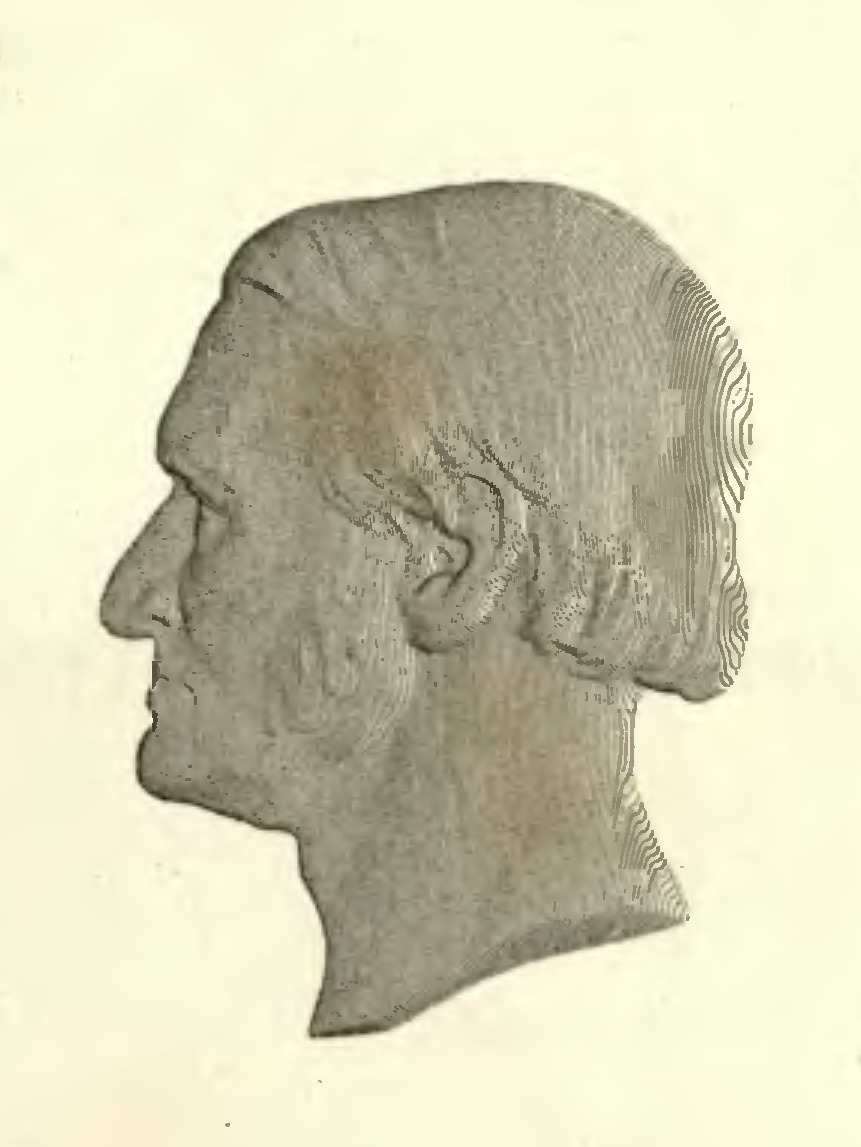
\includegraphics[height=1.93231in]{gauss_title_vignette_1870.jpg}\par
\medskip
HERAUSGEGEBEN\par
\smallskip
VON DER\par
\smallskip
KÖNIGLICHEN GESELLSCHAFT DER WISSENSCHAFTEN\par
\smallskip
ZU\par
\smallskip
\textls[180]{GÖTTINGEN.}\par
\medskip
IN COMMISSION BEI B. G. TEUBNER IN LEIPZIG.\par
\medskip
1900.
\end{center}
\clearpage

\SourceLeaf{7}% Otherwise blank verso bears a library ownership stamp, outside the historical body.

% Editionshinweis zur Übertragung ins heutige Deutsch.
\begin{center}\large Zu dieser Ausgabe\end{center}
\noindent Carl Friedrich Gauss, \emph{Werke}, Band VIII, Göttingen 1900.
Die Königliche Gesellschaft der Wissenschaften zu Göttingen gab die historische Ausgabe heraus.
Zu den historischen Herausgebern und Bearbeitern gehören Robert Fricke, Börsch, Krüger, Stäckel, Weingarten, Brendel und F. Klein.

\noindent Dieser Lesetext enthält die historischen Titelblätter und das Porträt
sowie die vollständige Abteilung Arithmetik und Algebra mit ihren Notizen und
Bemerkungen. Der Lesetext umfasst die gesamte Abteilung Analysis einschließlich der Fragmente über Modulfunktionen und das Pentagramma mirificum sowie die vollständigen Abteilungen Numerisches Rechnen und Wahrscheinlichkeitsrechnung. Die vollständigen Abteilungen Grundlagen der Geometrie, Geometria Situs und Elementare Geometrie umfassen den jeweiligen Nachlass, Briefwechsel, die Anzeigen und die gezeichneten Bemerkungen. Der Lesetext enthält auch die vollständigen Abteilungen über komplexe Größen in der Geometrie und zur Theorie der krummen Flächen sowie die historischen Bemerkungen, Berichtigungen, das Inhaltsverzeichnis und die Verlagsanzeige. Die gezeichneten Bemerkungen behalten ihre historischen Zuschreibungen. Der abgeschnittene rechte Teil der historischen Seite 95 folgt der alternativen Fotografie der Universität Kyūshū. Das Verhältnis der fotografierten Exemplare bleibt ungeklärt. Seitenverweise im Text beziehen sich auf die historische Ausgabe.

\noindent Übertragung ins heutige Deutsch und Satz durch OpenAI GPT-6.1 Sol (Ultra).
Transkription in den Originalsprachen und bearbeitbare mathematische Zeichnungen durch OpenAI GPT-6 Astra (Ultra).
Die unsignierte Titelvignette stammt aus dem \href{https://commons.wikimedia.org/w/index.php?oldid=1179960952}{zweiten Abdruck der \textit{Werke} I von 1870}, digitalisiert nach dem Exemplar der University of California Libraries. Dasselbe Motiv steht auf dem \href{https://gdz.sub.uni-goettingen.de/id/PPN236010751}{Göttinger Titelblatt von 1900}. \href{https://creativecommons.org/publicdomain/mark/1.0/}{Public Domain Mark 1.0}.
\clearpage

\SourceLeaf{8}
\thispagestyle{empty}
\vspace*{12em}
\begin{center}
{\Large ARITHMETIK UND ALGEBRA.\par}
\vspace{2em}
NACHTRÄGE ZU BAND I--III.
\end{center}
\clearpage

\SourceLeaf{9}% Blank historical verso, accounted without adding an empty reader page.

\SourceLeaf{10}
\begin{center}
{\Large NACHLASS.\par}
\bigskip
[ZWEI NOTIZEN ÜBER DIE LÖSUNG DER KONGRUENZ
\[
xx+yy+zz\equiv 0\quad(\mathrm{mod.}\ p).]
\]
\end{center}
\begin{center}[1.]\end{center}
\noindent\hspace*{\parindent}Jede Zerlegung einer durch die Primzahl $p$ teilbaren Zahl in vier Quadrate $=aa+bb+cc+dd$ entspricht einer Lösung der Kongruenz
\[
xx+yy+zz\equiv 0\quad(\mathrm{mod.}\ p).
\]
\noindent Zusammen gibt es $pp$ solcher Lösungen. Nimmt man die eine Lösung $x\equiv0$, $y\equiv0$, $z\equiv0$ davon weg, zerfallen die übrigen $pp-1$ in $p+1$ Klassen, wenn man $x=\xi$, $y=\eta$, $z=\zeta$ mit $x\equiv k\xi$, $y\equiv k\eta$, $z\equiv k\zeta$ zu einer Klasse zählt.

Es sind nämlich proportional
\[
\begin{array}{c|c|c|c}
x & aa+bb & -ad-bc & bd-ac\\
y & ac+bd & ab-cd & aa+dd\\
z & ad-bc & aa+cc & -ab-cd
\end{array}
\]
\begin{center}[2.]\end{center}
\noindent\hspace*{\parindent}Alle Lösungen der Kongruenz
\[
1+xx+yy\equiv0\quad(\mathrm{mod.}\ p)
\]
\noindent zu finden.
\clearpage

\SourceLeaf{11}
Es sind zugleich die Lösungen der Kongruenz
\[
1+(x+iy)^{p+1}\equiv0\quad\text{für}\quad p\equiv3\quad(\mathrm{mod.}\ 4).
\]
\par\indent Aus einem Wert $x+iy$ erhält man alle, indem man für $u$ alle Werte\\
$0,1,2,3,\, .\, .\, .,p-1$ einsetzt, und zwar mithilfe der Formel\HistoricalNote{[*)]}{[*)}{Neben dieser Herleitung stehen im Manuskript die Formeln:]
\[
1-xx\equiv yy,\qquad x=1-uy,\qquad 2u-uuy=y
\]
\[
\frac{1-uu}{1+uu}=x,\qquad\frac{2u}{1+uu}=y,
\]
\noindent [welche die Rolle des Zusatzfaktors $\dfrac{uu-1+2iu}{uu+1}$ erläutern.]}
\[
(x+iy)\left(\frac{uu-1+2iu}{uu+1}\right)\quad\text{oder}\quad\frac{(x+iy)(u+i)}{u-i}.
\]
\par\indent Für $p\equiv1\ (\mathrm{mod.}\ 4)=aa+bb$ enthält die Formel $\dfrac{b}{a}.\dfrac{u+i}{u-i}$ alle Werte von $x+iy$, wobei für $u$ nur die Werte $\dfrac{a}{b}$ und $\dfrac{b}{a}$ auszuschließen sind.

\clearpage\SourceLeaf{12}
\begin{center}\bfseries [NOTIZEN ÜBER KUBISCHE UND BIQUADRATISCHE RESTE.]\end{center}
\begin{center}[1.]\par\smallskip Eine höchst elegante, durch Induktion gewonnene Beobachtung.\end{center}
\noindent\hspace*{\parindent}2 ist ein kubischer Rest oder Nichtrest der Primzahl $p$ von der Form $3n+1$, je nachdem, ob $p$ darstellbar ist durch die Form
\[xx+27yy\qquad\text{oder}\qquad4xx+2xy+7yy.\]
\par\noindent\hspace*{\parindent}3 ist ein Rest oder Nichtrest, je nachdem, ob $p$ darstellbar ist durch
\[\begin{aligned} &xx+243yy\quad\text{oder}\quad4xx+2xy+61yy\\
\text{oder}\quad&7xx+6xy+36yy\quad\text{oder}\quad9xx+6xy+28yy.\end{aligned}\]
\par\noindent\hspace*{\parindent}5 ist ein $\left.\begin{array}{l}\text{Rest}\\\text{Nichtrest}\end{array}\right\}$, wenn $p$ dargestellt wird
\begingroup\small
\[\text{durch }\left\{\begin{array}{l}(1,0,675),\ (25,0,27),\ (13,1,52),\ (4,1,169)\\
(7,2,97),\ (9,3,76),\ (19,3,36),\ (25,5,28),\ (25,10,31),\ (27,9,28).\end{array}\right.\]
\endgroup
\begin{center}[2.]\end{center}
\noindent\hspace*{\parindent}Ein Kriterium, mit dem man entscheidet, ob die Zahl $m$ ein kubischer Rest der Primzahl $p$ von der Form $3n+1$ ist.

Es sei
\[4p=aa+27bb\]

\noindent\unskip\SourceLeaf{13}Dann gilt
\begin{center}\footnotesize\setlength{\tabcolsep}{3pt}
\begin{tabular}{@{}rlll@{}}
& &$m\ R\ p$&$m\ N\ p$\\
1)&$m=2$, wenn&$b$ gerade&$b$ ungerade\\
2)&$m=3$&$b$ teilb. durch 3&\\
3)&\multicolumn{3}{l}{$m={}$ eine andere Primzahl, wenn $\dfrac{a+b\sqrt{-27}}{a-b\sqrt{-27}}$ kubischer Rest von $m$}\\[5pt]
4)&\multicolumn{3}{l}{$m=6$, wenn entweder $2b$ oder $a+b$ oder $a-b$ durch 12 teilb.}\\
5)&\multicolumn{3}{l}{$m=10$, wenn entweder $2b$ oder $2a$ oder $a\pm3b$ oder $a\pm9b$ durch 20 teilb.}\\
6)&$m=12$&\multicolumn{2}{l}{$2b,\qquad a+5b,\qquad a-5b$ durch 12}\\
7)&$m=15$&\multicolumn{2}{l}{$b,\qquad 3a+5b,\qquad a\pm b,\qquad a\pm2b$ durch 15}\\
8)&$m=20$&\multicolumn{2}{l}{$2b,\qquad2a,\qquad a\pm b,\qquad a\pm7b$ durch 20}\\
9)&$m=45$&\multicolumn{2}{l}{$b,\qquad3a+5b,\qquad a\pm4b,\qquad a\pm7b$ durch 15}\\
10)&$m=14$&\multicolumn{2}{l}{$2b,\qquad2a,\qquad a\pm5b,\qquad a\pm11b$ durch 28}\\
11)&$m=28$&\multicolumn{2}{l}{$2b,\qquad2a,\qquad a\pm3b,\qquad a\pm9b$ durch 28.}
\end{tabular}\end{center}
\medskip
\par\noindent\hspace*{\parindent}Ein Kriterium, mit dem man entscheiden kann, ob die Zahl $m$ ein biquadratischer Rest der Primzahl $p$ von der Form $4n+1$ ist.

Es sei
\[p=aa+4bb\]
\Needspace{17\baselineskip}
\noindent Dann gilt $m\ R\ p$, wenn
\begin{center}\small\setlength{\tabcolsep}{3pt}\begin{tabular}{@{}rlll@{}}
1)&$m=-1$ wenn&$b$ gerade&$\pm4$ wenn $b$ gerade\\
2)&$m=\pm2$ wenn&$b$ durch 4 teilb.&$-4$ allgemein\\
3)&$m=+3$ wenn&$b$ oder $a+3b$ durch 6&\\
4)&$m=-3$ wenn&$b$ durch 3&\\
5)&$m=+5$ wenn&$b$ durch 5&\\
6)&$m=-5$ wenn&$b$ oder $a+5b$ durch 10&\\
7)&$m=+6$&\multicolumn{2}{l}{$b,\qquad2a+3b,\qquad a\pm b$ durch 12}\\
8)&$m=-6$&\multicolumn{2}{l}{$b,\qquad2a+3b,\qquad a\pm5b$ durch 12}\\
9)&$m=+7$&\multicolumn{2}{l}{$2a+7b,\qquad b,\qquad a\pm5b$ durch 14}
\end{tabular}\end{center}

\SourceLeaf{14}
\begin{center}\small\setlength{\tabcolsep}{3pt}\begin{tabular}{@{}rll@{}}
10)&$m=-7$&$a,\qquad b$ durch 7\\
11)&$m=+10$ wenn&$2a+5b,\qquad b,\qquad a\pm7b$ durch 20\\
12)&$m=-10$&$2a+5b,\qquad b,\qquad a\pm3b$ durch 20\\
13)&$m=+11$&$2a+11b,\qquad b,\qquad2a\pm3b,\qquad a\pm b$ durch 22\\
14)&$m=-11$&$b,\qquad a\pm4b$ durch 11.
\end{tabular}\end{center}
\begin{center}[3.]\par\smallskip Die kubischen Reste.\end{center}
\noindent\hspace*{\parindent}$p$ eine Primzahl der Form $3m+1$
\[4p=aa+27bb,\]
\par\noindent\hspace*{\parindent}$q$ eine andere Primzahl der Form $3n\pm1$
\[(a+3b\sqrt{-3})^{\frac{q\mp1}{3}}\equiv A\pm B\sqrt{-3}.\]
\par\noindent\hspace*{\parindent}Nun gibt es drei Fälle
\[\begin{array}{rlll}
\text{I.}&B\equiv0\quad\;(\mathrm{mod.}\ q).&\text{Dann ist }q^{\frac{p-1}{3}}\equiv1&\;(\mathrm{mod.}\ p).\\[5pt]
\text{II.}&B\equiv A\quad\;(\mathrm{mod.}\ q).&\text{Dann ist }q^{\frac{p-1}{3}}\equiv-\tfrac12-\tfrac12\dfrac{a}{3b}&\;(\mathrm{mod.}\ p).\\[5pt]
\text{III.}&B\equiv-A\quad\;(\mathrm{mod.}\ q).&\text{Dann ist }q^{\frac{p-1}{3}}\equiv-\tfrac12+\tfrac12\dfrac{a}{3b}&\;(\mathrm{mod.}\ p).
\end{array}\]
\Needspace{9\baselineskip}
\noindent\hspace*{\parindent}Erstes Beispiel.\qquad $\begin{array}[t]{ll}p=13,&q=5\\a=5,&b=1\end{array}$
\[(5+3\sqrt{-3})^2=-2+30\sqrt{-3},\quad B\equiv0\ \mathrm{mod.}\ 5\ \text{also Fall I}\]
\[5^4=625\equiv1.\]
\Needspace{9\baselineskip}
\noindent\hspace*{\parindent}Zweites Beispiel.\qquad $\begin{array}[t]{ll}p=19,&q=5\\a=7,&b=1\end{array}$
\[(7+3\sqrt{-3})^2=22+42\sqrt{-3},\quad B\equiv-A\ \text{also Fall III}\]
\[5^6\equiv7\quad\mathrm{mod.}\ 19,\qquad42\equiv-3+7\quad\mathrm{mod.}\ 19.\]

\Needspace{9\baselineskip}
\noindent\SourceLeaf{15}\hspace*{\parindent}Drittes Beispiel.\qquad $\begin{array}[t]{ll}p=7,&q=5\\a=1,&b=1\end{array}$
\[(1+3\sqrt{-3})^2=-26+6\sqrt{-3},\quad B\equiv+A\quad\mathrm{mod.}\ 5\quad\text{Fall II}\]
\[5^2\equiv4,\qquad24\equiv-3-1\quad\mathrm{mod.}\ 7.\]
\Needspace{9\baselineskip}
\noindent\hspace*{\parindent}Viertes Beispiel.\qquad $p=13,\qquad q=11$
\[(5+3\sqrt{-3})^4=-2696-120\sqrt{-3},\quad A\equiv-1,\quad B=120\equiv-1\]
\[11^4\equiv3,\qquad18+3\equiv-5\quad\mathrm{mod.}\ 13\quad\text{Fall II.}\]
\begin{center}Die biquadratischen Reste.\end{center}
\noindent\hspace*{\parindent}$p$ eine Primzahl von der Form $4n+1$
\[p=aa+4bb,\]
\par\noindent\hspace*{\parindent}$q$ eine Primzahl der Form $4n\pm1$
\[(a+2b\sqrt{-1})^{\frac{q\mp1}{4}}=A\pm B\sqrt{-1}.\]
\par\noindent\hspace*{\parindent}Nun gibt es vier Fälle
\[\begin{array}{rll}
\text{I.}&B\equiv0\ (\mathrm{mod.}\ q),&(\pm q)^{\frac{p-1}{4}}\equiv1\ (\mathrm{mod.}\ p).\\[4pt]
\text{II.}&A\equiv0&(\pm q)^{\frac{p-1}{4}}\equiv-1.\\[4pt]
\text{III.}&A\equiv B&(\pm q)^{\frac{p-1}{4}}\equiv-\dfrac{a}{2b}.\\[8pt]
\text{IV.}&A\equiv-B&(\pm q)^{\frac{p-1}{4}}\equiv\dfrac{a}{2b}.
\end{array}\]
\Needspace{9\baselineskip}
\noindent\hspace*{\parindent}Erstes Beispiel.\qquad $\begin{array}[t]{ll}p=13,&q=5\\a=3,&b=1\end{array}$
\[(3+2\sqrt{-1})^1=3+2\sqrt{-1},\quad A\equiv-B\quad\text{Fall IV}\]
\[5^3\equiv8\equiv\dfrac{3}{2.b}.\]
\Needspace{9\baselineskip}
\noindent\hspace*{\parindent}Zweites Beispiel.\qquad $p=13,\qquad q=7$
\[(3+2\sqrt{-1})^2=5+12\sqrt{-1},\quad A\equiv-B\quad\text{Fall IV}\]
\[(-7)^3\equiv8\equiv\dfrac{3}{2.b}.\]

\Needspace{9\baselineskip}
\noindent\SourceLeaf{16}\hspace*{\parindent}Drittes Beispiel.\qquad $p=13,\qquad q=11$
\[(3+2\sqrt{-1})^3=-9+46\sqrt{-1},\quad A\equiv-B\quad\text{Fall IV}\]
\[(-11)^3\equiv8\equiv\dfrac{3}{2.b}.\]
\Needspace{9\baselineskip}
\noindent\hspace*{\parindent}Viertes Beispiel.\qquad $p=17,\qquad q=11$
\[(1+4\sqrt{-1})^3=-47-52\sqrt{-1},\quad-47=A,\quad+52=B\]
\[A\equiv B\quad\text{Fall III}\]
\[(-11)^4\equiv4\equiv-\tfrac14.\]
\begin{center}[4.]\end{center}
\noindent\hspace*{\parindent}Es sei $p$ eine Primzahl, $n$ eine Primzahl $=3m+1$, $R$ Wurzel der Gleichung $x^3-1=0$, $r$ Wurzel der Gleichung $r^n-1=0$, $g$ Primitivwurzel modulo $n$.
\[r+Rr^g+R^2r^{g^2}+R^3r^{g^3}+\ldots+R^{n-2}r^{g^{n-2}}=P,\]
\[P^3=\tfrac12 n(M+N\sqrt{-27}),\]
\noindent wo
\[M\equiv1\ (\mathrm{mod.}\ 3),\qquad0\equiv M+3N(g^m-g^{2m})\ (\mathrm{mod.}\ n)\]
\[3k=M+2\]
\[a=\tfrac19(n+1+M)\]
\[b-c=N.\]
\[P^{pp}\equiv r^{pp}+Rr^{ppg}+\ldots\equiv P(R^{\mathrm{ind.}\,p})\]
\begingroup\footnotesize
\[\begin{array}{r@{}l|c}
&1&0\\[3pt]
\{\tfrac12 n(M+N\sqrt{-27})\}^{\frac13(pp-1)}\equiv{}&-\tfrac12+\tfrac12\sqrt{-3}\ (\mathrm{mod.}\ p)&\mathrm{ind.}\ p\equiv1\ (\mathrm{mod.}\ 3)\\[3pt]
&-\tfrac12-\tfrac12\sqrt{-3}&2
\end{array}\]
\endgroup
\[4n=(M+N\sqrt{-27})(M-N\sqrt{-27})\]
\[\dfrac{M}{3N}\equiv g^{2m}-g^m,\qquad-1\equiv g^{2m}+g^m\]
\begingroup\footnotesize
\[\begin{array}{r@{}l|c}
&1&1\\[3pt]
\left\{\dfrac{M-N\sqrt{-27}}{M+N\sqrt{-27}}\right\}^{\frac13(pp-1)}\equiv{}&-\tfrac12+\tfrac12\sqrt{-3}\ (\mathrm{mod.}\ p)&p^{\frac13(n-1)}\equiv-\tfrac12-\tfrac12\dfrac{M}{3N}\ (\mathrm{mod.}\ n)\\[5pt]
&-\tfrac12-\tfrac12\sqrt{-3}&-\tfrac12+\tfrac12\dfrac{M}{3N}
\end{array}\]
\endgroup

\SourceLeaf{17}
\[P^4\equiv PR^{\mathrm{ind.}\,2}\]
\[\tfrac12 M+\tfrac32 N(R-R^2)=\tfrac12(M+3N)+3NR\]
\[\begin{array}{r@{}l|cc}
&1&\tfrac12(M+3N)\ \text{ungerade}&3N\ \text{gerade}\\[4pt]
2^{\frac13(n-1)}\equiv{}&-\tfrac12+\tfrac12\dfrac{M}{3N}\ (\mathrm{mod.}\ n)&\text{ungerade}&\text{ungerade}\\[5pt]
&-\tfrac12-\tfrac12\dfrac{M}{3N}&\text{gerade}&\text{ungerade.}
\end{array}\]
\begin{center}Für den kubischen Rest 3.\end{center}
\[\begin{aligned}
p^3&=m(a-1)+\{m+(a-1)^2+bb+cc\}p\\
&\qquad+\{(a-1)b+bc+ac\}p'\\
&\qquad+\{(a-1)c+ab+bc\}p''\\
&=A+Bp+Cp'+Dp''.
\end{aligned}\]
\noindent Nun ist
\[\begin{array}{rl}1)&aa+bb+cc=ab+ac+bc+a\\2)&a+b+c=m\\3)&3k-2=M\\4)&4a=kk+3NN\\5)&4n=(3k-2)^2+27NN\\6)&4m=3kk-4k+9NN.\end{array}\]
\noindent Hieraus folgt
\[\begin{aligned}A&\equiv0\quad\;(\mathrm{mod.}\ 3)\\ B&=\tfrac13(mm-a)-a+m+1\\ C&=\tfrac13(mm-a)-b\\D&=\tfrac13(mm-a)-c\end{aligned}\]
\[\begin{aligned}\tfrac43(mm-a)&\equiv-2k^3+kk-NN\quad\;(\mathrm{mod.}\ 3)\\
&\equiv kk+k-NN\quad\;(\mathrm{mod.}\ 3)\\
&\equiv4a-4m-NN\quad\;(\mathrm{mod.}\ 3).\end{aligned}\]

\noindent\unskip\SourceLeaf{18}Also
\[\begin{aligned}B&\equiv-NN+1\equiv-(b-c)^2+1\\C&\equiv-NN+b-c\equiv-(b-c)^2+b-c\\D&\equiv-NN-(b-c)\equiv-(b-c)^2-(b-c)\end{aligned}\]
\[\begin{array}{rrrr}
b-c\equiv0&B\equiv1&C\equiv0&D\equiv0\\1&0&0&1\\2&0&1&0.
\end{array}\]
\par\noindent\hspace*{\parindent}Ist also 3 ein Rest modulo $n$, so ist $N$ durch 3 teilbar.
\Needspace{10\baselineskip}
\begingroup\small
\begin{center}BEMERKUNGEN ZU DEN VORSTEHENDEN NOTIZEN ÜBER KUBISCHE UND BIQUADRATISCHE RESTE.\end{center}
\noindent\hspace*{\parindent}Die Notiz [1] ist von \textsc{Gauss} auf das Vorsatzblatt des Einbandes seines Handexemplars der Disquisitiones arithmeticae geschrieben. Die Angaben unter [2] finden sich in einem mit der Überschrift »Uraniae sacrum« versehenen Hefte, und ebenda folgen zwei Seiten später die beiden allgemeinen Sätze [3]. Die Entwicklungen unter [4] sind einigen losen Zetteln entnommen.

\textsc{Gauss} gibt zu Beginn seiner Commentatio prima über die Theorie der biquadratischen Reste an, dass er mit dem Jahre 1805 begonnen habe, die Theorie der kubischen und biquadratischen Reste zu durchforschen. Die hier unter [2] und [3] gegebenen Entwicklungen folgen in dem genannten Hefte unmittelbar auf Notizen, welche das Datum 1804 tragen. Die »Observatio venustissima« [1], welche weniger weitreichend ist als die »Criterien« [2] und [3], kann zeitlich nicht wohl später liegen als Letztere. Man wird es demnach hier mit den ältesten \textsc{Gauss}'schen Untersuchungen und damit überhaupt mit den ältesten Urkunden über die höheren Reziprozitätsgesetze zu tun haben.

Wie die Observatio, so sind vermutlich auch die Kriterien Induktionsresultate. Es ist aber sehr bemerkenswert, dass schon hier bei den Kriterien die Zerlegung der quadratischen Form $aa+27bb$ in ihre beiden komplexen Faktoren und damit der Zahl $p$ in ihre beiden komplexen Primteiler auftritt. Es war bereits hiermit die Bahn gewonnen, auf welcher \textsc{Gauss} späterhin wenigstens das biquadratische Reziprozitätsgesetz in seine einfachste Gestalt kleidete. Bei gewissen Beweisansätzen des allgemeinen kubischen Reziprozitätsgesetzes (siehe die gleich folgenden Notizen), welche jedenfalls vor 1809 liegen, ist übrigens \textsc{Gauss} wenigstens am Beginn allein vom Gebrauch rationaler Zahlen ausgegangen.

Die zu Anfang von [2] unter 3) gemachte Angabe lässt sich als Spezialfall aus dem ersten allgemeinen Satze unter [3] entnehmen. Letzterer liefert direkt das Reziprozitätsgesetz in der allgemeinsten und einfachsten Gestalt, falls $p=3m+1$ und $q=3n-1$ ist. Der kubische Charakter des Primteiler $\pi_1=\dfrac{a+3b\sqrt{-3}}{2}$ in Bezug auf $q$ ist nämlich durch
\[\left[\frac{\pi_1}{q}\right]\equiv(A-B\sqrt{-3})^{q-1}\quad\;(\mathrm{mod.}\ q)\]

\noindent\unskip\SourceLeaf{19}angegeben, ein Ausdruck, der entweder mit 1, $\rho$ oder $\rho^2$ modulo $q$ kongruent ist, unter $\rho$ die Einheitswurzel
$\dfrac{-1+i\sqrt{3}}{2}$ verstanden. Da nun im Gebiete der aus $\rho$ zu bildenden ganzen komplexen Zahlen die Lösungen
der Kongruenz $x^{q-1}\equiv 1\;(\mathrm{mod.}\ q)$ die $(q-1)$ von 0 verschiedenen rationalen ganzen Reste modulo $q$ sind,
so kommt die von \textsc{Gauss} vermöge der Kongruenzen $B\equiv 0$, $B\equiv A$, $B\equiv -A\;(\mathrm{mod.}\ q)$ vollzogene Dreiteilung darauf hinaus, dass der kubische Charakter $\left[\dfrac{\pi_1}{q}\right]$ gleich 1 bzw. $\rho$, $\rho^2$ ist. Im anderen Falle $q=3n+1$
ist hier der einfachste Ausdruck des Reziprozitätsgesetzes deshalb noch nicht erreicht, weil die Zerlegung von
$q$ in seine Primteiler noch nicht vollzogen ist. Die Beziehung des \textsc{Gauss}'schen Theorems zum Reziprozitätsgesetz ist die folgende.

Sind die Zerlegungen der rationalen Primzahlen $p, q$ in ihre primären Primfaktoren gegeben durch
\[ p=\pi_1.\pi_2,\qquad q=\varkappa_1.\varkappa_2,\qquad \pi_k'=2\pi_k=a\pm 3b\sqrt{-3}, \]
so hat man zu setzen
\[
\left.\begin{array}{l}
\left[\dfrac{\pi_1'}{\varkappa_1}\right]=\rho^{\varepsilon_1}\equiv {\pi_1'}^{\frac{q-1}{3}}\equiv A+B\rho-B\rho^2 \\[2mm]
\left[\dfrac{\pi_2'}{\varkappa_1}\right]=\rho^{\varepsilon_2}\equiv {\pi_2'}^{\frac{q-1}{3}}\equiv A-B\rho+B\rho^2
\end{array}\right\}(\mathrm{mod.}\ \varkappa_1).
\]

\noindent Die \textsc{Gauss}'sche Dreiteilung kommt dann mit der folgenden überein
\[
\text{I.}\quad \varepsilon_1\equiv \varepsilon_2 (\mathrm{mod.}\ 3),\qquad \left[\dfrac{\pi_1'}{\varkappa_1}\right]=\left[\dfrac{\pi_2'}{\varkappa_1}\right],
\]
\[
\text{II.}\quad \varepsilon_1\equiv \varepsilon_2+1\;(\mathrm{mod.}\ 3),\qquad \left[\dfrac{\pi_1'}{\varkappa_1}\right]=\rho\left[\dfrac{\pi_2'}{\varkappa_1}\right],
\]
\[
\text{III.}\quad \varepsilon_1\equiv \varepsilon_2-1\;(\mathrm{mod.}\ 3),\qquad \left[\dfrac{\pi_1'}{\varkappa_1}\right]=\rho^2\left[\dfrac{\pi_2'}{\varkappa_1}\right],
\]
wobei in den drei letzten Gleichungen offenbar auch $\pi_k$ an Stelle von $\pi_k'$ treten kann. Liegt nämlich z.\,B.
der Fall II vor, so folgt durch Addition und Subtraktion obiger Kongruenzen in Bezug auf den Modul $\varkappa_1$
\[
2A\equiv \rho^{\varepsilon_2}(1+\rho)\equiv -\rho^{\varepsilon_2-1},\qquad 2B\equiv -\rho^{\varepsilon_2-1}\qquad\;(\mathrm{mod.}\ \varkappa_1),
\]
so dass $(A-B)$ durch $\varkappa_1$ und als rationale Zahl demnach auch durch $q$ teilbar ist. Man hat also wirklich $B\equiv A\;(\mathrm{mod.}\ q)$. Das Reziprozitätsgesetz liefert nun
\[
\left[\dfrac{\pi_1'}{\varkappa_1}\right]=\left[\dfrac{2}{\varkappa_1}\right].\left[\dfrac{\pi_1}{\varkappa_1}\right]=\left[\dfrac{2}{\varkappa_1}\right].\left[\dfrac{\varkappa_1}{\pi_1}\right],
\]
\[
\left[\dfrac{\pi_2'}{\varkappa_1}\right]=\left[\dfrac{2}{\varkappa_1}\right].\left[\dfrac{\pi_2}{\varkappa_1}\right]=\left[\dfrac{2}{\varkappa_1}\right].\left[\dfrac{\varkappa_1}{\pi_2}\right],
\]
so dass man für den Fall II weiter gewinnt
\[
\left[\dfrac{\varkappa_1}{\pi_1}\right]=\rho\left[\dfrac{\varkappa_1}{\pi_2}\right]=\rho\left[\dfrac{\varkappa_2}{\pi_1}\right]^2,\qquad
\left[\dfrac{\varkappa_1}{\pi_1}\right].\left[\dfrac{\varkappa_2}{\pi_1}\right]=\left[\dfrac{q}{\pi_1}\right]=\rho,
\]
\[
\left[\dfrac{q}{\pi_1}\right]\equiv q^{\frac{p-1}{3}}\equiv -\tfrac12+\tfrac12\sqrt{-3}\equiv -\tfrac12-\tfrac12\dfrac{a}{3b}\qquad\;(\mathrm{mod.}\ \pi_1).
\]
Soll aber die rationale Zahl $q^{\frac{p-1}{3}}+\tfrac12+\tfrac12\dfrac{a}{3b}\equiv 0 \mathrm{mod.}\ \pi_1$ sein, so ist sie auch durch $\pi_2$ und also durch $p$
teilbar. Hiermit ist die unter II von \textsc{Gauss} angegebene Kongruenz in Bezug auf den Modul $p$ gewonnen.
Ebenso erledigen sich die Fälle I und III.

\SourceLeaf{20}

Die Umkehrung der vorstehenden Entwicklung lehrt, dass man aus den Angaben von \textsc{Gauss} im
Fall $q=3n+1$ zunächst auf die Proportion
\[
\left[\dfrac{\varkappa_1}{\pi_1}\right]:\left[\dfrac{\pi_1}{\varkappa_1}\right]=\left[\dfrac{\varkappa_1}{\pi_2}\right]:\left[\dfrac{\pi_2}{\varkappa_1}\right]
\]
schließen kann. Unter nochmaliger Benutzung des in dieser Proportion ausgesprochenen Gesetzes findet man
\[
\dfrac{\left[\dfrac{\varkappa_1}{\pi_1}\right]}{\left[\dfrac{\pi_1}{\varkappa_1}\right]}=\dfrac{\left[\dfrac{\varkappa_2}{\pi_1}\right]}{\left[\dfrac{\pi_1}{\varkappa_2}\right]}=\dfrac{\left[\dfrac{\varkappa_1}{\pi_2}\right]^2}{\left[\dfrac{\pi_2}{\varkappa_1}\right]^2}
\quad\text{und also}\quad
\dfrac{\left[\dfrac{\varkappa_1}{\pi_2}\right]}{\left[\dfrac{\pi_2}{\varkappa_1}\right]}=\dfrac{\left[\dfrac{\varkappa_1}{\pi_2}\right]^3}{\left[\dfrac{\pi_2}{\varkappa_1}\right]^2}.
\]
Da hieraus $\left[\dfrac{\varkappa_1}{\pi_2}\right]=\left[\dfrac{\pi_2}{\varkappa_1}\right]$ hervorgeht, ist auch für $q=3n+1$ in den Angaben von \textsc{Gauss} das allgemeine Reziprozitätsgesetz in seiner einfachsten Form implizit enthalten.

Unter [4] sind diejenigen Aufzeichnungen gesammelt, durch die \textsc{Gauss} seine kubischen Reziprozitätstheoreme bewiesen hat. Da diese Aufzeichnungen mehreren losen Zetteln ohne Datumsangabe entnommen sind, lässt sich die Entstehungszeit der fraglichen Beweise nicht mit Sicherheit angeben. Es ist
aber wahrscheinlich, dass die Entwicklungen bald nach Gewinnung der »Observatio« und der »Criterien«
durchgeführt wurden. Sie schließen sich nämlich im Gedankengang sehr eng an die ersten Angaben unter [2]
und im Übrigen an Art. 358 der Disquisitiones arithmeticae an. Andererseits war \textsc{Gauss} zufolge seiner
eigenen Aussage\HistoricalNote{\textsuperscript{*)}}{*)}{Siehe Art. 33 der am 24. August 1808 der Göttinger Societät vorgelegten Abhandlung »Summatio quarumdam serierum singularium«.} jedenfalls vor Mitte des Jahres 1808 im Besitz des sechsten Beweises des quadratischen
Reziprozitätsgesetzes, der mit den hier gemeinten Beweisen am nächsten verwandt ist.

Dem Beweis von \textsc{Gauss} für das kubische Reziprozitätsgesetz liegt die Kreisteilung zugrunde. Die
einzelnen Formeln unter [4] können entweder unmittelbar aus Art. 358 der Disquisitiones arithmeticae entnommen werden oder lassen sich zumindest mit sehr geringer Mühe aus den dortigen Entwicklungen ableiten.
Die Kongruenz
\[
P^{pp}\equiv r^{pp}+Rr^{ppg}+\ldots\equiv P(R^{\mathrm{ind.}\,p})
\]
bezieht sich auf den Modul $p$ und ergibt sich daraus, dass alle von 1 verschiedenen Polynomkoeffizienten der Potenz $pp$ durch $p$ teilbar sind. Die Fallunterscheidung
\[
\left\{\dfrac{M-N\sqrt{-27}}{M+N\sqrt{-27}}\right\}^{\frac13(pp-1)}\equiv 1,\quad -\tfrac12+\tfrac12\sqrt{-3},\quad -\tfrac12-\tfrac12\sqrt{-3}\qquad\;(\mathrm{mod.}\ p)
\]
entspricht sowohl für $p=3m-1$ als auch für $p=3m+1$ genau der oben unter I, II und III getroffenen
Unterscheidung $B\equiv 0\;(\mathrm{mod.}\ q)$ usw. Die Zuordnung jener drei Kongruenzen zu den folgenden
\[
p^{\frac13(n-1)}\equiv 1,\quad -\tfrac12-\tfrac12\dfrac{M}{3N},\quad -\tfrac12+\tfrac12\dfrac{M}{3N}\qquad\;(\mathrm{mod.}\ n),
\]
wie sie in [4] entwickelt wird, enthält demnach bereits einen vollständigen Beweis der Angaben von \textsc{Gauss}
und damit implizit des allgemeinen kubischen Reziprozitätsgesetzes.

Die weiteren Ausführungen unter [4] betreffen die Kriterien dafür, dass 2 und 3 kubische Reste sind.
Zum kubischen Rest 3 bemerke man nur, dass (unter Verwendung der in [4] gebrauchten Bezeichnung)
$p^3\equiv p, p'$ oder $p''\;(\mathrm{mod.}\ 3)$ zutrifft, je nachdem, ob ind.\,$3\equiv 0, 1$ oder $2\;(\mathrm{mod.}\ 3)$ gilt. Die Bedingung
$N\equiv 0\;(\mathrm{mod.}\ 3)$ dafür, dass 3 kubischer Rest modulo $n$ ist, ergibt sich daraufhin unmittelbar aus den Schlussangaben von [4].


\SourceLeaf{21}

Die Observatio kann aus den Criterien leicht abgeleitet werden. Z.\,B. wurde für den kubischen Rest 3
soeben die Bedingung $N\equiv 0\;(\mathrm{mod.}\ 3)$ gewonnen und unter [2] ebenso angegeben. Sind nun $M$ und $N$
gerade, so setze man
\[ M=2x,\qquad N=6y, \]
sodass aus $4n=M^2+27N^2$ die Darstellbarkeit von $n$ durch die quadratische Form mit der Determinante $-243$
\[ n=x^2+243y^2 \]
mit ganzzahligen $x, y$ folgt. Umgekehrt folgt aus der Möglichkeit einer solchen Darstellung von $n$
die Gültigkeit der Kongruenz $N\equiv 0\;(\mathrm{mod.}\ 3)$. Sind $M$ und $N$ ungerade, so wähle man das Vorzeichen richtig und setze
\[ M\pm\dfrac{N}{3}=4x,\qquad \mp\dfrac{N}{3}=y, \]
woraus man die Darstellung
\[ n=4x^2+2xy+61y^2. \]
gewinnt. Aus dieser Formel würde umgekehrt $N\equiv 0\;(\mathrm{mod.}\ 3)$ folgen, sodass 3 genau dann kubischer Rest
modulo $n$ ist, wenn $n$ durch eine der Formen $(1,0,243)$, $(4,1,61)$ darstellbar ist.

Herr R. \textsc{Dedekind}, dem ich mehrere für mich sehr förderliche Unterhaltungen über die in
Rede stehenden Gegenstände verdanke, hat mich darauf aufmerksam gemacht, dass für den Fall des kubischen
Nichtrests 3 modulo $n$ die Angaben von \textsc{Gauss} nicht ganz vollständig sind. Es gibt insgesamt neun Klassen ursprünglicher Formen erster Art mit der Determinante $D=-243$, deren reduzierte Formen die folgenden sind
\[ (1,0,243),\quad (4,\pm1,61),\quad (13,\pm2,19),\quad (7,\pm3,36),\quad (9,\pm3,28). \]
In [1] fehlen die Formen $(13,\pm2,19)$. Das Theorem muss demnach so lauten, dass 3 genau
dann kubischer Nichtrest modulo $n$ ist, wenn $n$ eine Darstellung in einer der folgenden Formen gestattet
\[ n=13xx+4xy+19yy, \]
\[ n=7xx+6xy+36yy, \]
\[ n=9xx+6xy+28yy. \]
Diese Darstellungen erhält man stets, indem man bei den folgenden Transformationen das Vorzeichen richtig wählt
\[ \text{I. Wenn } M\equiv N\equiv 1\;(\mathrm{mod.}\ 2),\quad M\pm 7N\equiv 0\;(\mathrm{mod.}\ 12), \]
\[ M=5x+7y,\qquad \pm N=x-y. \]
\[ \text{II. Wenn } M\equiv N\equiv 1\;(\mathrm{mod.}\ 2),\quad M\pm 7N\equiv 6\;(\mathrm{mod.}\ 12), \]
\[ M=x+6y,\qquad \mp N=x. \]
\[ \text{III. Wenn } M\equiv N\equiv 0\;(\mathrm{mod.}\ 2),\quad M\pm N\equiv 0\;(\mathrm{mod.}\ 3), \]
\[ M=6x+2y,\qquad \mp N=2y. \]
\par\noindent\hspace*{\parindent}Die Angaben zur Zahl 5 unter 1 folgen in ähnlicher Weise aus dem Restkriterium
$MN\equiv 0\;(\mathrm{mod.}\ 5)$.

Im Übrigen sei noch bemerkt, dass sich im Original der Notiz [1] eine bis 223 fortgesetzte Tabelle derjenigen Primzahlen $p=3n+1$ findet, für die die Zahlen 2, 3, 5, 7 kubische Reste sind.

\hfill \textsc{Fricke.}

\endgroup

\clearpage\SourceLeaf{22}
\begin{center}
\bfseries ZUR THEORIE DER KUBISCHEN RESTE.
\end{center}



\begin{center}
[1.]
\end{center}

\[ p=mm+3nn \text{ eine Primzahl.} \]

\noindent\hspace*{\parindent}Für eine beliebige, durch $p$ nicht teilbare ganze Zahl $x$ setze man
\[
\left[\dfrac{2mx}{p}\right]=\alpha,\qquad \left[\dfrac{(3n-m)x}{p}\right]=\beta,\qquad \left[\dfrac{(-3n-m)x}{p}\right]=\gamma.
\]
\noindent Hieraus ergibt sich, wie man leicht sieht,
\[
\dfrac{2mx}{p}-\alpha+\dfrac{(3n-m)x}{p}-\beta+\dfrac{(-3n-m)x}{p}-\gamma
\]
als Summe dreier echter Brüche. Sie muss daher strikt zwischen den
Grenzen 0 und 3 liegen. Da diese Summe aber offenbar $=-\alpha-\beta-\gamma$, also
eine ganze Zahl ist, kann sie nur die Werte $+1$ und $+2$ annehmen.
Es gilt also entweder
\[ \alpha+\beta+\gamma=-1\quad\text{oder}\quad \alpha+\beta+\gamma=-2. \]

\noindent Hieraus folgt ferner, dass die Größen $\alpha, \beta, \gamma$ nicht alle drei zueinander
modulo 3 kongruent sein können. Unter den Differenzen $\alpha-\beta$, $\beta-\gamma$,
$\gamma-\alpha$ wird also mindestens eine (und eben deshalb mindestens noch eine,

\SourceLeaf{23}
weil ihre Summe $=0$ ist) sein, die nicht $\equiv 0$ ist. Ebenso wenig
können aber die Größen $\alpha, \beta, \gamma$ alle zueinander inkongruent sein.
Sonst müssten sie, gleichgültig in welcher Reihenfolge, zu den Zahlen
$0, 1, 2$ kongruent und ihre Summe daher durch $3$ teilbar sein. Folglich
ist unter den Differenzen $\alpha-\beta$,
$\beta-\gamma$, $\gamma-\alpha$ genau eine, die
$\equiv 0$ ist. Es gibt somit drei Fälle, die sich gegenseitig ausschließen:

\[
\text{I.} \quad \text{Wenn } \beta \equiv \gamma \quad(\mathrm{mod.}\ 3)
\]
\[
\text{II.} \quad \text{Wenn } \gamma \equiv \alpha \quad(\mathrm{mod.}\ 3)
\]
\[
\text{III.} \quad \text{Wenn } \alpha \equiv \beta \quad(\mathrm{mod.}\ 3).
\]

Welcher dieser drei Fälle eintritt, hängt von $x$ ab. Wir teilen daher
alle durch $p$ nicht teilbaren Zahlen nach diesen drei Fällen in drei
Klassen ein. In die erste kommen diejenigen, bei denen der erste Fall eintritt,
in die zweite diejenigen, bei denen der zweite eintritt, und in die dritte
diejenigen, bei denen der dritte eintritt.

\textls[100]{Erster Satz:} Alle modulo $p$ kongruenten Zahlen gehören
derselben Klasse an.

\textls[100]{Zweiter Satz:} Zahlen mit gleichem Betrag und entgegengesetzten
Vorzeichen gehören derselben Klasse an.

Daraus ist klar, dass man nur die Zahlen $1, 2, 3, \ldots,
\frac{1}{2}(p-1)$
klassifizieren muss, um sofort alle übrigen klassifizieren zu können.

\textls[100]{Dritter Satz:} Die Zahlen $(3n-m)x$ und $2mx$ gehören zwei
aufeinanderfolgenden Klassen an.

\textls[100]{Vierter Satz:} Gilt also $\dfrac{2n-m}{3m} \equiv f$ und damit

\[
1+f+ff \equiv 0 \quad(\mathrm{mod.}\ p), \qquad 1 \equiv f^3 \quad(\mathrm{mod.}\ p),
\]
\noindent so gehören $x$ und die Reste von $fx$ und $ffx$
drei in umgekehrter Reihenfolge aufeinanderfolgenden Klassen an.


\clearpage\SourceLeaf{24}
\begin{center}\textls[100]{Beispiele zur Einteilung.}\end{center}


\begingroup\small
\[p = 7 = 4+3, \qquad 4,\quad 1,\quad -5\]
\begin{center}\begin{tabular}{@{}rl@{}}
I. & 3.\ 4.\\
II. & 2.\ 5.\\
III. & 1.\ 6.\end{tabular}\end{center}
\[p = 13 = 1+12, \qquad 2,\quad 5,\quad -7\]
\begin{center}\begin{tabular}{@{}rl@{}}
I. & 3.\ 6.\ 7.\ 10.\\
II. & 4.\ 5.\ 8.\ 9.\\
III. & 1.\ 2.\ 11.\ 12.\end{tabular}\end{center}
\[p = 19 = 16+3, \qquad 8,\quad -1,\quad -7\]
\begin{center}\begin{tabular}{@{}rl@{}}
I. & 1.\ 2.\ 9.\ 10.\ 17.\ 18.\\
II. & 3.\ 4.\ 8.\ 11.\ 15.\ 16.\\
III. & 5.\ 6.\ 7.\ 12.\ 13.\ 14.\end{tabular}\end{center}
\[p = 31 = 4+27, \qquad 4,\quad 7,\quad -11\]
\begin{center}\begin{tabular}{@{}rl@{}}
I. & 5.\ 9.\ 10.\ 11.\ 15.\ 16.\ 20.\ 21.\ 22.\ 26.\\
II. & 6.\ 7.\ 12.\ 13.\ 14.\ 17.\ 18.\ 19.\ 24.\ 25.\\
III. & 1.\ 2.\ 3.\ 4.\ 8.\ 23.\ 27.\ 28.\ 29.\ 30.\end{tabular}\end{center}
\[p = 37 = 25+12, \qquad 10,\quad 1,\quad -11\]
\begin{center}\begin{tabular}{@{}rl@{}}
I. & 7.\ 8.\ 9,\ 10.\ 17.\ 18.\ 19.\ 20.\ 27.\ 28.\ 29.\ 30.\\
II. & 4.\ 5.\ 6.\ 11.\ 15.\ 16.\ 21.\ 22.\ 26.\ 31.\ 32.\ 33.\\
III. & 1.\ 2.\ 3.\ 12.\ 13.\ 14.\ 23.\ 24.\ 25.\ 34.\ 35.\ 36.\end{tabular}\end{center}
\[p = 43 = 16+27, \qquad 8,\quad 5,\quad -13\]
\begin{center}\begin{tabular}{@{}rl@{}}
I. & 7.\ 8.\ 14.\ 15.\ 16.\ 20.\ 21.\ 22.\ 23.\ 27.\ 28.\ 29.\ 35.\ 36.\\
II. & 6.\ 11.\ 12.\ 13.\ 17.\ 18.\ 19.\ 24.\ 25.\ 26.\ 30.\ 31.\ 32.\ 37.\\
III. & 1.\ 2.\ 3.\ 4.\ 5.\ 9.\ 10.\ 33.\ 34.\ 38.\ 39.\ 40.\ 41.\ 42.\end{tabular}\end{center}
\begin{center}
\begin{tabular}[t]{c|c|c}
\multicolumn{3}{c}{$7,\quad2-\rho$}\\\hline
$1$&$-\rho\rho$&$\rho$\\
$-1$&$\rho\rho$&$-\rho$
\end{tabular}\qquad
\begin{tabular}[t]{c|c|c}
\multicolumn{3}{c}{$13,\quad3-\rho$}\\\hline
$1$&$1-\rho$&$-\rho\rho$\\
$1-\rho\rho$&$\rho$&$\rho-\rho\rho$\\
$-1$&$-1+\rho$&$\rho\rho$\\
$-1+\rho\rho$&$-\rho$&$-\rho+\rho\rho$
\end{tabular}
\end{center}\endgroup

\clearpage\SourceLeaf{25}
\begin{center}\begin{tikzpicture}[x=.195pt,y=-.195pt]
\path[use as bounding box] (0,0) rectangle (1750,1100);
\path[fill=black,even odd rule] (414,171) -- (413,174) -- (411,176) -- (411,181) -- (408,185) -- (408,188) -- (406,192) -- (406,197) -- (405,198) -- (405,209) -- (403,212) -- (403,218) -- (401,221) -- (401,224) -- (400,225) -- (399,231) -- (396,235) -- (396,237) -- (394,239) -- (394,241) -- (387,249) -- (386,252) -- (383,255) -- (382,258) -- (379,261) -- (379,262) -- (376,265) -- (375,265) -- (374,267) -- (355,285) -- (355,286) -- (351,290) -- (348,295) -- (344,299) -- (344,302) -- (342,306) -- (340,308) -- (339,308) -- (338,310) -- (338,313) -- (336,315) -- (334,319) -- (333,325) -- (331,327) -- (331,329) -- (330,330) -- (330,334) -- (328,336) -- (326,340) -- (326,343) -- (324,345) -- (322,349) -- (322,351) -- (321,352) -- (321,354) -- (322,355) -- (319,359) -- (319,362) -- (318,363) -- (317,368) -- (311,379) -- (311,382) -- (309,384) -- (309,389) -- (308,390) -- (307,397) -- (305,400) -- (305,403) -- (303,405) -- (302,416) -- (301,417) -- (301,422) -- (299,425) -- (299,429) -- (297,431) -- (297,434) -- (295,437) -- (295,439) -- (292,442) -- (292,445) -- (290,448) -- (290,451) -- (289,452) -- (290,456) -- (289,457) -- (289,464) -- (288,465) -- (289,467) -- (289,469) -- (288,470) -- (288,474) -- (290,478) -- (290,484) -- (291,485) -- (291,491) -- (292,492) -- (291,496) -- (292,497) -- (293,509) -- (294,510) -- (294,513) -- (295,514) -- (295,520) -- (296,521) -- (296,527) -- (297,528) -- (297,532) -- (296,533) -- (296,535) -- (297,536) -- (297,547) -- (298,548) -- (297,551) -- (298,552) -- (298,556) -- (299,557) -- (299,578) -- (301,580) -- (301,582) -- (302,583) -- (302,587) -- (304,590) -- (304,592) -- (307,595) -- (306,599) -- (308,603) -- (308,609) -- (309,610) -- (309,612) -- (311,614) -- (311,618) -- (313,620) -- (314,626) -- (317,631) -- (318,654) -- (319,655) -- (318,678) -- (317,679) -- (317,686) -- (315,689) -- (315,691) -- (311,695) -- (311,698) -- (309,700) -- (309,702) -- (308,703) -- (308,709) -- (307,710) -- (307,713) -- (308,714) -- (307,715) -- (307,719) -- (308,720) -- (308,723) -- (310,726) -- (310,729) -- (314,737) -- (314,739) -- (317,743) -- (316,744) -- (317,754) -- (316,755) -- (316,760) -- (315,761) -- (315,763) -- (316,764) -- (315,765) -- (315,769) -- (313,773) -- (315,777) -- (316,793) -- (322,805) -- (324,807) -- (324,809) -- (326,811) -- (326,817) -- (327,818) -- (327,821) -- (329,823) -- (329,826) -- (331,830) -- (331,844) -- (330,846) -- (332,848) -- (332,852) -- (331,853) -- (331,855) -- (332,856) -- (332,862) -- (335,869) -- (335,873) -- (337,875) -- (339,881) -- (344,886) -- (344,888) -- (352,896) -- (352,897) -- (369,913) -- (370,916) -- (378,926) -- (381,933) -- (387,940) -- (388,943) -- (393,948) -- (396,953) -- (396,955) -- (399,958) -- (400,963) -- (404,967) -- (405,973) -- (407,975) -- (408,980) -- (413,988) -- (430,1003) -- (434,1005) -- (439,1010) -- (443,1011) -- (446,1015) -- (448,1016) -- (451,1016) -- (454,1018) -- (457,1018) -- (458,1019) -- (462,1019) -- (463,1020) -- (472,1021) -- (475,1023) -- (481,1023) -- (482,1024) -- (488,1024) -- (489,1025) -- (491,1025) -- (492,1024) -- (510,1024) -- (511,1023) -- (518,1023) -- (519,1022) -- (522,1022) -- (528,1019) -- (530,1017) -- (532,1017) -- (533,1016) -- (537,1016) -- (538,1015) -- (541,1015) -- (542,1014) -- (546,1014) -- (547,1013) -- (550,1014) -- (551,1013) -- (562,1012) -- (563,1011) -- (577,1011) -- (582,1014) -- (584,1013) -- (589,1013) -- (590,1014) -- (599,1015) -- (601,1017) -- (603,1017) -- (607,1019) -- (610,1019) -- (612,1021) -- (616,1021) -- (618,1023) -- (621,1022) -- (622,1023) -- (626,1023) -- (627,1024) -- (655,1024) -- (656,1023) -- (664,1023) -- (668,1021) -- (680,1021) -- (681,1020) -- (684,1020) -- (685,1019) -- (699,1019) -- (700,1018) -- (705,1018) -- (709,1016) -- (714,1016) -- (717,1014) -- (721,1014) -- (725,1012) -- (735,1011) -- (736,1010) -- (742,1010) -- (743,1009) -- (747,1009) -- (748,1008) -- (750,1008) -- (754,1010) -- (757,1007) -- (768,1006) -- (770,1004) -- (772,1004) -- (775,1002) -- (778,1002) -- (781,1000) -- (788,1000) -- (789,999) -- (792,999) -- (793,998) -- (798,998) -- (800,997) -- (801,998) -- (808,998) -- (809,999) -- (823,1000) -- (824,1001) -- (827,1001) -- (834,1005) -- (837,1005) -- (841,1007) -- (845,1007) -- (847,1009) -- (851,1010) -- (858,1016) -- (859,1016) -- (868,1025) -- (869,1025) -- (874,1030) -- (875,1030) -- (881,1037) -- (883,1037) -- (884,1038) -- (889,1038) -- (896,1042) -- (899,1045) -- (904,1045) -- (905,1046) -- (910,1047) -- (912,1049) -- (918,1052) -- (921,1055) -- (923,1055) -- (930,1060) -- (932,1060) -- (936,1064) -- (940,1064) -- (945,1068) -- (947,1068) -- (953,1072) -- (961,1073) -- (962,1074) -- (968,1074) -- (970,1076) -- (978,1077) -- (981,1079) -- (1000,1079) -- (1001,1078) -- (1007,1078) -- (1009,1076) -- (1014,1075) -- (1017,1073) -- (1021,1073) -- (1026,1070) -- (1028,1070) -- (1034,1067) -- (1042,1066) -- (1044,1064) -- (1047,1064) -- (1048,1065) -- (1051,1065) -- (1052,1064) -- (1056,1064) -- (1057,1065) -- (1068,1065) -- (1069,1064) -- (1075,1064) -- (1080,1061) -- (1085,1061) -- (1088,1059) -- (1092,1059) -- (1093,1058) -- (1110,1057) -- (1114,1055) -- (1115,1056) -- (1117,1056) -- (1118,1055) -- (1122,1055) -- (1123,1054) -- (1132,1053) -- (1136,1050) -- (1142,1049) -- (1147,1046) -- (1151,1046) -- (1154,1044) -- (1159,1044) -- (1160,1043) -- (1168,1042) -- (1169,1041) -- (1174,1041) -- (1175,1040) -- (1186,1040) -- (1189,1038) -- (1191,1038) -- (1192,1039) -- (1194,1038) -- (1203,1038) -- (1204,1037) -- (1209,1037) -- (1210,1036) -- (1218,1036) -- (1219,1035) -- (1225,1035) -- (1226,1034) -- (1231,1034) -- (1232,1033) -- (1244,1033) -- (1245,1032) -- (1249,1032) -- (1250,1031) -- (1253,1031) -- (1254,1030) -- (1257,1030) -- (1258,1029) -- (1261,1029) -- (1262,1028) -- (1271,1028) -- (1274,1026) -- (1293,1026) -- (1294,1025) -- (1301,1025) -- (1305,1023) -- (1307,1024) -- (1315,1024) -- (1316,1023) -- (1321,1023) -- (1322,1024) -- (1324,1024) -- (1327,1022) -- (1336,1022) -- (1340,1020) -- (1349,1020) -- (1350,1019) -- (1354,1019) -- (1355,1018) -- (1360,1017) -- (1362,1015) -- (1365,1014) -- (1366,1012) -- (1370,1012) -- (1371,1011) -- (1374,1011) -- (1375,1010) -- (1378,1010) -- (1379,1009) -- (1382,1009) -- (1383,1008) -- (1386,1008) -- (1387,1007) -- (1395,1007) -- (1396,1006) -- (1399,1006) -- (1403,1008) -- (1411,1008) -- (1415,1010) -- (1429,1010) -- (1430,1011) -- (1434,1011) -- (1435,1012) -- (1438,1012) -- (1439,1011) -- (1447,1011) -- (1448,1012) -- (1460,1012) -- (1464,1010) -- (1468,1010) -- (1472,1008) -- (1475,1004) -- (1477,1003) -- (1480,1003) -- (1485,1000) -- (1488,1000) -- (1492,997) -- (1494,997) -- (1496,995) -- (1499,994) -- (1502,991) -- (1504,991) -- (1514,983) -- (1519,981) -- (1524,975) -- (1528,973) -- (1534,973) -- (1535,972) -- (1537,972) -- (1542,968) -- (1544,968) -- (1547,966) -- (1549,966) -- (1553,963) -- (1560,961) -- (1562,959) -- (1566,958) -- (1567,956) -- (1572,955) -- (1574,953) -- (1575,950) -- (1579,946) -- (1581,946) -- (1583,944) -- (1584,944) -- (1587,940) -- (1588,940) -- (1593,936) -- (1593,934) -- (1601,927) -- (1603,923) -- (1609,917) -- (1609,912) -- (1611,909) -- (1611,898) -- (1612,897) -- (1612,894) -- (1614,892) -- (1614,884) -- (1615,883) -- (1615,878) -- (1616,877) -- (1616,872) -- (1615,871) -- (1617,869) -- (1618,861) -- (1620,859) -- (1620,843) -- (1621,842) -- (1621,839) -- (1622,838) -- (1623,829) -- (1625,826) -- (1625,817) -- (1626,816) -- (1626,810) -- (1625,809) -- (1626,808) -- (1626,801) -- (1625,800) -- (1626,797) -- (1624,793) -- (1624,789) -- (1622,786) -- (1622,778) -- (1621,777) -- (1621,774) -- (1620,773) -- (1622,771) -- (1622,769) -- (1620,767) -- (1620,764) -- (1622,762) -- (1622,751) -- (1623,750) -- (1623,745) -- (1624,744) -- (1624,741) -- (1623,740) -- (1623,735) -- (1621,733) -- (1621,727) -- (1620,726) -- (1620,718) -- (1621,717) -- (1621,715) -- (1619,713) -- (1619,709) -- (1620,708) -- (1619,706) -- (1619,704) -- (1620,703) -- (1620,697) -- (1621,696) -- (1621,694) -- (1623,692) -- (1623,689) -- (1624,688) -- (1624,682) -- (1626,680) -- (1626,678) -- (1628,676) -- (1629,668) -- (1631,666) -- (1632,662) -- (1634,660) -- (1634,657) -- (1638,649) -- (1638,645) -- (1645,636) -- (1646,630) -- (1647,629) -- (1647,624) -- (1650,620) -- (1650,617) -- (1651,616) -- (1654,593) -- (1656,591) -- (1653,585) -- (1653,582) -- (1651,580) -- (1651,575) -- (1647,568) -- (1647,562) -- (1645,560) -- (1645,556) -- (1644,554) -- (1642,553) -- (1641,547) -- (1639,544) -- (1639,541) -- (1638,540) -- (1639,539) -- (1639,532) -- (1638,531) -- (1638,525) -- (1637,524) -- (1637,520) -- (1636,519) -- (1637,517) -- (1637,515) -- (1636,514) -- (1636,505) -- (1637,504) -- (1639,493) -- (1642,490) -- (1642,486) -- (1644,482) -- (1647,479) -- (1648,475) -- (1658,463) -- (1658,461) -- (1661,456) -- (1665,452) -- (1665,449) -- (1666,448) -- (1666,446) -- (1669,442) -- (1669,439) -- (1673,434) -- (1674,430) -- (1675,429) -- (1675,421) -- (1676,420) -- (1676,416) -- (1678,412) -- (1678,406) -- (1680,404) -- (1680,399) -- (1681,398) -- (1682,391) -- (1684,389) -- (1685,383) -- (1688,377) -- (1688,374) -- (1689,373) -- (1690,368) -- (1693,364) -- (1694,356) -- (1696,354) -- (1697,349) -- (1699,347) -- (1699,345) -- (1701,343) -- (1703,339) -- (1703,336) -- (1706,331) -- (1707,326) -- (1709,323) -- (1709,319) -- (1710,318) -- (1710,314) -- (1711,313) -- (1710,311) -- (1710,306) -- (1711,305) -- (1711,296) -- (1710,295) -- (1711,293) -- (1711,285) -- (1710,284) -- (1710,282) -- (1711,281) -- (1711,279) -- (1710,278) -- (1710,270) -- (1708,268) -- (1708,266) -- (1710,264) -- (1710,263) -- (1708,261) -- (1708,256) -- (1706,254) -- (1705,246) -- (1702,240) -- (1702,235) -- (1701,234) -- (1702,231) -- (1700,229) -- (1700,226) -- (1698,224) -- (1698,221) -- (1697,219) -- (1694,216) -- (1689,208) -- (1687,207) -- (1687,204) -- (1684,200) -- (1684,194) -- (1682,190) -- (1679,187) -- (1677,182) -- (1672,176) -- (1672,173) -- (1666,167) -- (1666,166) -- (1663,163) -- (1662,160) -- (1657,155) -- (1657,153) -- (1655,149) -- (1640,130) -- (1638,126) -- (1631,120) -- (1631,119) -- (1624,111) -- (1624,110) -- (1622,108) -- (1621,108) -- (1620,106) -- (1608,94) -- (1605,89) -- (1603,88) -- (1602,85) -- (1590,74) -- (1586,73) -- (1584,71) -- (1577,71) -- (1573,69) -- (1556,69) -- (1555,70) -- (1553,69) -- (1533,69) -- (1532,68) -- (1528,68) -- (1524,66) -- (1514,65) -- (1511,63) -- (1506,62) -- (1502,59) -- (1498,59) -- (1495,57) -- (1492,57) -- (1488,54) -- (1483,54) -- (1482,53) -- (1478,54) -- (1477,53) -- (1467,53) -- (1466,52) -- (1462,52) -- (1461,53) -- (1454,53) -- (1453,52) -- (1438,53) -- (1437,52) -- (1435,52) -- (1434,53) -- (1427,53) -- (1426,54) -- (1420,54) -- (1419,55) -- (1413,55) -- (1412,56) -- (1403,57) -- (1399,59) -- (1391,60) -- (1390,61) -- (1383,62) -- (1379,64) -- (1376,64) -- (1368,68) -- (1357,68) -- (1356,69) -- (1350,68) -- (1349,69) -- (1345,69) -- (1344,70) -- (1343,69) -- (1325,68) -- (1324,67) -- (1320,67) -- (1319,66) -- (1311,66) -- (1310,65) -- (1288,65) -- (1287,66) -- (1282,66) -- (1281,67) -- (1278,67) -- (1271,70) -- (1262,71) -- (1261,72) -- (1255,73) -- (1254,74) -- (1248,74) -- (1243,77) -- (1236,78) -- (1232,80) -- (1220,80) -- (1219,81) -- (1213,81) -- (1212,82) -- (1207,82) -- (1206,83) -- (1203,83) -- (1202,84) -- (1196,84) -- (1193,86) -- (1190,86) -- (1189,87) -- (1185,87) -- (1184,88) -- (1180,88) -- (1179,89) -- (1170,89) -- (1169,90) -- (1161,91) -- (1160,92) -- (1153,92) -- (1152,93) -- (1148,93) -- (1147,92) -- (1130,92) -- (1129,91) -- (1117,91) -- (1116,90) -- (1114,91) -- (1109,91) -- (1108,90) -- (1105,90) -- (1104,89) -- (1082,89) -- (1078,91) -- (1073,91) -- (1072,92) -- (1069,92) -- (1065,94) -- (1062,94) -- (1061,95) -- (1058,95) -- (1057,96) -- (1049,97) -- (1048,98) -- (1046,98) -- (1042,100) -- (1039,100) -- (1035,102) -- (1028,102) -- (1027,103) -- (1024,103) -- (1023,104) -- (1016,104) -- (1013,106) -- (1010,105) -- (1009,106) -- (1005,106) -- (1004,107) -- (998,107) -- (997,106) -- (989,106) -- (988,107) -- (983,107) -- (982,106) -- (971,106) -- (968,104) -- (959,103) -- (956,101) -- (954,101) -- (950,99) -- (939,97) -- (935,94) -- (931,94) -- (929,92) -- (922,89) -- (916,84) -- (914,84) -- (906,80) -- (902,80) -- (900,78) -- (892,74) -- (889,74) -- (885,72) -- (882,72) -- (869,63) -- (866,62) -- (859,56) -- (856,55) -- (851,51) -- (849,51) -- (842,45) -- (840,44) -- (837,44) -- (834,41) -- (831,41) -- (826,38) -- (823,38) -- (819,35) -- (809,35) -- (808,34) -- (804,35) -- (803,34) -- (800,34) -- (799,33) -- (796,33) -- (795,34) -- (793,34) -- (792,33) -- (763,33) -- (762,32) -- (760,32) -- (759,33) -- (754,33) -- (753,32) -- (741,32) -- (740,31) -- (737,31) -- (736,32) -- (734,31) -- (728,31) -- (727,32) -- (726,31) -- (723,31) -- (722,30) -- (703,30) -- (702,31) -- (699,31) -- (698,30) -- (692,30) -- (691,29) -- (688,29) -- (687,30) -- (673,30) -- (672,31) -- (665,31) -- (664,30) -- (662,30) -- (661,29) -- (659,29) -- (652,26) -- (650,27) -- (649,26) -- (642,26) -- (641,25) -- (613,25) -- (612,26) -- (603,26) -- (601,28) -- (599,28) -- (598,27) -- (595,29) -- (591,29) -- (589,31) -- (572,31) -- (566,34) -- (559,35) -- (557,37) -- (554,38) -- (546,45) -- (545,45) -- (538,52) -- (536,53) -- (533,53) -- (527,56) -- (524,56) -- (521,58) -- (519,58) -- (515,62) -- (513,62) -- (508,66) -- (505,67) -- (501,71) -- (499,71) -- (494,76) -- (493,76) -- (476,90) -- (475,92) -- (475,95) -- (469,100) -- (466,108) -- (463,111) -- (463,113) -- (458,119) -- (458,121) -- (456,125) -- (454,127) -- (453,130) -- (450,133) -- (450,134) -- (441,144) -- (438,145) -- (436,147) -- (436,148) -- (418,165) -- (417,168) -- cycle (1012,991) -- (1012,1022) -- (1013,1023) -- (1013,1025) -- (1012,1026) -- (1013,1028) -- (1012,1030) -- (1012,1034) -- (1013,1035) -- (1013,1039) -- (1012,1040) -- (1012,1042) -- (1013,1043) -- (1013,1062) -- (1014,1063) -- (1013,1064) -- (1013,1068) -- (1014,1070) -- (1012,1072) -- (1009,1072) -- (1008,1073) -- (1002,1073) -- (999,1075) -- (993,1075) -- (992,1076) -- (984,1076) -- (980,1074) -- (974,1074) -- (973,1073) -- (970,1073) -- (969,1072) -- (962,1072) -- (954,1068) -- (952,1068) -- (945,1063) -- (940,1062) -- (934,1057) -- (920,1050) -- (915,1045) -- (921,1040) -- (924,1039) -- (926,1037) -- (928,1037) -- (934,1034) -- (940,1029) -- (942,1029) -- (943,1028) -- (948,1028) -- (958,1019) -- (960,1019) -- (962,1017) -- (969,1014) -- (974,1010) -- (978,1009) -- (985,1003) -- (988,1002) -- (990,1000) -- (992,1000) -- (994,998) -- (996,998) -- (1000,996) -- (1003,992) -- (1005,991) -- (1008,991) -- (1009,990) -- (1011,990) -- cycle (1015,988) -- (1016,987) -- (1018,987) -- (1021,990) -- (1028,993) -- (1033,997) -- (1037,998) -- (1042,1004) -- (1046,1004) -- (1048,1005) -- (1051,1008) -- (1062,1013) -- (1066,1017) -- (1068,1017) -- (1070,1019) -- (1072,1019) -- (1075,1022) -- (1077,1022) -- (1082,1027) -- (1084,1028) -- (1088,1028) -- (1090,1030) -- (1095,1032) -- (1100,1036) -- (1102,1036) -- (1105,1039) -- (1108,1040) -- (1110,1042) -- (1118,1046) -- (1120,1046) -- (1121,1048) -- (1117,1051) -- (1112,1051) -- (1105,1054) -- (1099,1054) -- (1098,1055) -- (1091,1055) -- (1090,1056) -- (1081,1057) -- (1080,1058) -- (1078,1058) -- (1076,1060) -- (1073,1060) -- (1070,1062) -- (1044,1061) -- (1041,1063) -- (1036,1063) -- (1035,1064) -- (1029,1065) -- (1023,1068) -- (1020,1068) -- (1017,1065) -- (1017,1029) -- (1016,1028) -- (1016,1018) -- (1017,1017) -- (1017,1015) -- (1016,1014) -- (1016,1005) -- (1015,1004) -- (1015,996) -- (1016,995) -- (1016,991) -- (1015,990) -- cycle (1507,790) -- (1509,790) -- (1511,792) -- (1515,794) -- (1517,794) -- (1520,797) -- (1523,798) -- (1528,802) -- (1538,807) -- (1540,809) -- (1542,809) -- (1547,814) -- (1549,814) -- (1551,816) -- (1553,816) -- (1555,818) -- (1557,818) -- (1559,820) -- (1561,820) -- (1565,824) -- (1569,825) -- (1572,828) -- (1577,830) -- (1580,833) -- (1586,836) -- (1588,836) -- (1596,842) -- (1599,843) -- (1602,846) -- (1605,846) -- (1607,847) -- (1614,853) -- (1614,856) -- (1613,857) -- (1613,864) -- (1612,865) -- (1611,875) -- (1610,876) -- (1610,884) -- (1609,885) -- (1608,893) -- (1607,894) -- (1607,899) -- (1606,900) -- (1606,906) -- (1605,907) -- (1602,918) -- (1600,920) -- (1598,924) -- (1589,933) -- (1589,934) -- (1587,936) -- (1583,938) -- (1569,950) -- (1565,951) -- (1559,954) -- (1556,957) -- (1554,957) -- (1551,959) -- (1547,960) -- (1544,963) -- (1541,963) -- (1537,966) -- (1535,966) -- (1534,967) -- (1530,967) -- (1525,970) -- (1523,970) -- (1511,981) -- (1508,978) -- (1508,956) -- (1509,955) -- (1508,954) -- (1508,936) -- (1509,934) -- (1508,933) -- (1508,930) -- (1507,929) -- (1507,927) -- (1508,926) -- (1507,924) -- (1507,919) -- (1508,918) -- (1508,908) -- (1507,907) -- (1507,905) -- (1508,904) -- (1508,902) -- (1507,901) -- (1508,897) -- (1507,896) -- (1507,889) -- (1508,888) -- (1508,885) -- (1507,884) -- (1507,873) -- (1506,872) -- (1507,870) -- (1507,858) -- (1506,857) -- (1506,844) -- (1507,843) -- (1507,841) -- (1505,839) -- (1506,836) -- (1505,835) -- (1505,820) -- (1504,819) -- (1505,818) -- (1505,801) -- (1504,800) -- (1504,798) -- (1505,797) -- (1505,792) -- cycle (1573,901) -- (1573,903) -- (1575,905) -- (1583,905) -- (1586,902) -- (1586,900) -- (1583,897) -- (1578,897) -- cycle (1501,789) -- (1501,791) -- (1502,792) -- (1501,794) -- (1501,816) -- (1502,817) -- (1502,822) -- (1501,823) -- (1502,825) -- (1502,829) -- (1501,830) -- (1501,832) -- (1502,833) -- (1502,841) -- (1501,842) -- (1501,850) -- (1502,851) -- (1501,861) -- (1502,862) -- (1502,868) -- (1501,869) -- (1501,871) -- (1502,872) -- (1502,888) -- (1503,889) -- (1503,891) -- (1501,894) -- (1502,896) -- (1502,903) -- (1501,905) -- (1503,908) -- (1503,941) -- (1504,942) -- (1503,944) -- (1504,946) -- (1503,947) -- (1504,949) -- (1503,951) -- (1503,968) -- (1504,969) -- (1504,974) -- (1503,975) -- (1503,978) -- (1504,979) -- (1504,982) -- (1500,987) -- (1499,987) -- (1496,990) -- (1493,991) -- (1488,995) -- (1485,995) -- (1477,999) -- (1475,999) -- (1465,1005) -- (1460,1005) -- (1457,1007) -- (1456,1006) -- (1453,1006) -- (1451,1007) -- (1450,1006) -- (1447,1006) -- (1446,1005) -- (1429,1006) -- (1428,1005) -- (1424,1005) -- (1423,1004) -- (1411,1004) -- (1410,1003) -- (1406,1003) -- (1405,1002) -- (1383,1002) -- (1382,1003) -- (1378,1003) -- (1377,1004) -- (1375,1004) -- (1372,1006) -- (1368,1006) -- (1366,1008) -- (1364,1008) -- (1361,1010) -- (1358,1010) -- (1356,1012) -- (1352,1014) -- (1348,1014) -- (1341,1017) -- (1326,1017) -- (1325,1018) -- (1304,1018) -- (1303,1019) -- (1287,1019) -- (1286,1020) -- (1284,1019) -- (1283,1020) -- (1280,1020) -- (1279,1021) -- (1271,1021) -- (1270,1022) -- (1264,1021) -- (1263,1022) -- (1260,1022) -- (1256,1024) -- (1253,1024) -- (1246,1027) -- (1235,1027) -- (1234,1026) -- (1234,1025) -- (1236,1023) -- (1236,1021) -- (1235,1020) -- (1233,1020) -- (1232,1019) -- (1222,1019) -- (1220,1022) -- (1220,1025) -- (1222,1027) -- (1218,1030) -- (1210,1030) -- (1209,1031) -- (1205,1031) -- (1201,1033) -- (1193,1033) -- (1192,1034) -- (1189,1034) -- (1188,1035) -- (1179,1035) -- (1178,1036) -- (1171,1036) -- (1170,1037) -- (1166,1037) -- (1165,1038) -- (1160,1038) -- (1157,1040) -- (1151,1040) -- (1150,1041) -- (1145,1042) -- (1142,1044) -- (1140,1044) -- (1136,1046) -- (1127,1047) -- (1125,1045) -- (1123,1045) -- (1118,1041) -- (1115,1040) -- (1110,1036) -- (1108,1036) -- (1104,1034) -- (1101,1031) -- (1095,1028) -- (1093,1026) -- (1095,1024) -- (1095,1022) -- (1090,1019) -- (1084,1019) -- (1083,1020) -- (1081,1020) -- (1074,1015) -- (1070,1014) -- (1064,1009) -- (1062,1009) -- (1058,1007) -- (1056,1005) -- (1054,1005) -- (1051,1002) -- (1049,1002) -- (1047,1000) -- (1043,999) -- (1041,997) -- (1033,993) -- (1031,991) -- (1027,990) -- (1024,987) -- (1021,986) -- (1019,984) -- (1021,982) -- (1027,980) -- (1032,976) -- (1034,976) -- (1038,973) -- (1040,973) -- (1042,971) -- (1046,970) -- (1046,969) -- (1049,966) -- (1053,964) -- (1056,964) -- (1067,956) -- (1071,955) -- (1075,953) -- (1078,950) -- (1080,950) -- (1084,948) -- (1089,944) -- (1091,944) -- (1094,941) -- (1095,941) -- (1097,939) -- (1099,939) -- (1101,937) -- (1103,937) -- (1106,934) -- (1109,933) -- (1115,928) -- (1119,928) -- (1124,924) -- (1129,922) -- (1130,920) -- (1132,919) -- (1136,919) -- (1140,915) -- (1142,915) -- (1145,912) -- (1147,912) -- (1151,909) -- (1154,909) -- (1155,908) -- (1161,908) -- (1163,907) -- (1165,905) -- (1165,903) -- (1169,899) -- (1173,898) -- (1174,896) -- (1176,896) -- (1181,892) -- (1188,889) -- (1193,885) -- (1196,884) -- (1199,881) -- (1201,881) -- (1205,879) -- (1208,876) -- (1211,876) -- (1213,874) -- (1221,871) -- (1224,868) -- (1227,868) -- (1228,870) -- (1231,870) -- (1237,873) -- (1240,876) -- (1254,883) -- (1256,885) -- (1263,887) -- (1267,891) -- (1269,891) -- (1272,894) -- (1274,894) -- (1276,896) -- (1279,897) -- (1282,900) -- (1285,900) -- (1287,901) -- (1289,903) -- (1289,905) -- (1290,906) -- (1298,908) -- (1300,907) -- (1311,895) -- (1316,894) -- (1320,891) -- (1323,891) -- (1330,885) -- (1333,885) -- (1337,881) -- (1341,880) -- (1343,878) -- (1346,877) -- (1355,870) -- (1358,870) -- (1363,866) -- (1365,866) -- (1369,864) -- (1373,860) -- (1375,860) -- (1379,856) -- (1384,856) -- (1387,853) -- (1390,852) -- (1393,849) -- (1396,848) -- (1401,844) -- (1415,837) -- (1418,834) -- (1428,830) -- (1431,827) -- (1432,827) -- (1440,821) -- (1446,819) -- (1449,816) -- (1454,813) -- (1456,813) -- (1459,810) -- (1462,809) -- (1464,807) -- (1467,807) -- (1469,805) -- (1471,805) -- (1475,803) -- (1477,801) -- (1482,799) -- (1484,797) -- (1486,797) -- (1494,790) -- (1498,788) -- (1500,788) -- cycle (1428,903) -- (1432,907) -- (1436,908) -- (1440,906) -- (1443,903) -- (1443,900) -- (1439,898) -- (1433,898) -- (1431,899) -- cycle (1612,722) -- (1614,722) -- (1616,724) -- (1616,727) -- (1617,728) -- (1617,734) -- (1619,738) -- (1619,746) -- (1618,747) -- (1618,753) -- (1619,754) -- (1619,756) -- (1618,757) -- (1618,760) -- (1617,761) -- (1616,785) -- (1617,786) -- (1617,788) -- (1619,789) -- (1619,794) -- (1620,795) -- (1620,798) -- (1622,801) -- (1622,803) -- (1621,804) -- (1621,818) -- (1620,819) -- (1620,829) -- (1619,830) -- (1619,834) -- (1618,835) -- (1618,840) -- (1617,841) -- (1616,845) -- (1614,847) -- (1610,846) -- (1608,844) -- (1603,842) -- (1595,836) -- (1590,834) -- (1588,832) -- (1586,832) -- (1580,827) -- (1576,826) -- (1571,822) -- (1568,821) -- (1565,818) -- (1562,817) -- (1558,813) -- (1553,811) -- (1551,809) -- (1547,808) -- (1545,806) -- (1541,805) -- (1537,802) -- (1535,802) -- (1533,800) -- (1530,799) -- (1523,794) -- (1518,792) -- (1516,790) -- (1514,790) -- (1510,786) -- (1512,781) -- (1515,778) -- (1520,776) -- (1523,773) -- (1526,773) -- (1528,771) -- (1533,769) -- (1537,765) -- (1539,765) -- (1545,762) -- (1548,759) -- (1550,759) -- (1554,756) -- (1557,756) -- (1561,752) -- (1565,752) -- (1565,751) -- (1569,747) -- (1573,747) -- (1579,744) -- (1581,742) -- (1582,742) -- (1586,737) -- (1591,736) -- (1597,731) -- (1599,731) -- (1603,728) -- (1607,727) -- cycle (596,673) -- (599,671) -- (603,672) -- (607,674) -- (610,677) -- (616,680) -- (618,682) -- (620,682) -- (622,684) -- (625,684) -- (629,688) -- (631,688) -- (633,690) -- (635,690) -- (638,693) -- (641,694) -- (647,699) -- (649,699) -- (651,701) -- (660,705) -- (665,709) -- (671,712) -- (672,714) -- (676,715) -- (679,718) -- (685,721) -- (687,723) -- (690,724) -- (692,726) -- (699,729) -- (701,731) -- (703,731) -- (706,734) -- (710,735) -- (717,741) -- (724,744) -- (730,749) -- (733,749) -- (738,753) -- (746,756) -- (749,759) -- (753,760) -- (757,764) -- (760,764) -- (764,768) -- (769,770) -- (771,772) -- (775,774) -- (777,774) -- (784,780) -- (787,780) -- (789,782) -- (793,783) -- (795,785) -- (799,787) -- (801,789) -- (801,792) -- (802,793) -- (801,795) -- (801,798) -- (802,799) -- (802,809) -- (803,810) -- (802,812) -- (802,837) -- (801,838) -- (801,841) -- (802,842) -- (802,854) -- (803,856) -- (800,859) -- (800,860) -- (804,864) -- (807,864) -- (810,867) -- (815,869) -- (817,871) -- (821,873) -- (823,873) -- (829,879) -- (831,879) -- (833,881) -- (839,883) -- (841,885) -- (847,888) -- (850,891) -- (852,891) -- (855,894) -- (857,894) -- (859,896) -- (861,896) -- (863,898) -- (866,899) -- (869,902) -- (869,903) -- (870,904) -- (872,904) -- (875,908) -- (877,909) -- (884,909) -- (886,910) -- (894,917) -- (896,917) -- (898,919) -- (901,919) -- (906,923) -- (909,924) -- (912,927) -- (916,928) -- (921,932) -- (926,934) -- (929,937) -- (932,937) -- (934,938) -- (937,941) -- (940,942) -- (946,947) -- (953,950) -- (959,955) -- (961,955) -- (965,957) -- (968,960) -- (977,964) -- (979,966) -- (982,967) -- (989,972) -- (993,973) -- (996,976) -- (998,976) -- (1003,980) -- (1009,982) -- (1010,983) -- (1009,986) -- (1005,989) -- (1001,990) -- (997,992) -- (995,994) -- (990,996) -- (988,998) -- (985,999) -- (978,1004) -- (973,1006) -- (971,1008) -- (966,1010) -- (963,1013) -- (959,1014) -- (956,1017) -- (954,1017) -- (949,1020) -- (947,1020) -- (946,1019) -- (944,1020) -- (937,1020) -- (937,1021) -- (935,1023) -- (936,1027) -- (934,1029) -- (932,1029) -- (929,1032) -- (926,1033) -- (924,1035) -- (915,1039) -- (911,1043) -- (907,1041) -- (902,1040) -- (897,1036) -- (889,1035) -- (881,1028) -- (875,1025) -- (873,1021) -- (868,1018) -- (860,1010) -- (856,1008) -- (850,1003) -- (845,1002) -- (842,1000) -- (831,999) -- (826,996) -- (819,995) -- (817,993) -- (808,993) -- (807,992) -- (798,992) -- (797,993) -- (791,993) -- (787,995) -- (782,995) -- (780,997) -- (768,999) -- (764,1002) -- (755,1002) -- (754,1003) -- (749,1003) -- (745,1005) -- (737,1006) -- (733,1008) -- (714,1009) -- (711,1011) -- (707,1011) -- (706,1012) -- (703,1012) -- (699,1014) -- (690,1014) -- (689,1015) -- (686,1015) -- (685,1016) -- (676,1016) -- (675,1017) -- (662,1017) -- (661,1018) -- (658,1018) -- (657,1019) -- (641,1019) -- (640,1020) -- (631,1020) -- (630,1019) -- (624,1019) -- (623,1018) -- (614,1017) -- (613,1016) -- (605,1014) -- (602,1012) -- (596,1011) -- (593,1009) -- (587,1009) -- (586,1008) -- (574,1008) -- (573,1007) -- (567,1007) -- (566,1008) -- (557,1008) -- (556,1009) -- (548,1009) -- (547,1010) -- (538,1010) -- (537,1011) -- (534,1011) -- (533,1012) -- (527,1012) -- (526,1011) -- (526,989) -- (527,987) -- (526,986) -- (526,956) -- (525,955) -- (526,953) -- (526,948) -- (528,946) -- (536,943) -- (536,942) -- (539,939) -- (541,939) -- (543,937) -- (547,936) -- (558,928) -- (562,927) -- (565,924) -- (571,921) -- (573,921) -- (579,918) -- (581,916) -- (583,916) -- (586,913) -- (592,910) -- (595,910) -- (602,905) -- (602,904) -- (599,901) -- (599,898) -- (598,897) -- (598,895) -- (599,894) -- (598,890) -- (599,888) -- (595,883) -- (598,881) -- (598,876) -- (596,874) -- (599,869) -- (599,864) -- (597,860) -- (599,858) -- (599,853) -- (600,852) -- (600,849) -- (599,848) -- (599,838) -- (598,837) -- (599,833) -- (597,831) -- (597,822) -- (598,821) -- (597,808) -- (599,806) -- (598,804) -- (598,800) -- (597,799) -- (597,797) -- (598,796) -- (598,788) -- (597,787) -- (597,784) -- (598,782) -- (597,780) -- (599,777) -- (599,774) -- (598,773) -- (598,767) -- (597,766) -- (597,752) -- (599,750) -- (599,749) -- (598,748) -- (598,737) -- (597,736) -- (597,732) -- (598,731) -- (598,720) -- (597,719) -- (597,709) -- (596,708) -- (597,706) -- (597,697) -- (596,696) -- (597,694) -- (597,690) -- (596,689) -- (597,688) -- (597,679) -- (596,678) -- cycle (727,903) -- (727,906) -- (729,909) -- (740,909) -- (744,905) -- (744,904) -- (739,899) -- (733,899) -- (732,900) -- (730,900) -- cycle (662,782) -- (662,787) -- (665,789) -- (669,789) -- (671,790) -- (675,786) -- (675,782) -- (673,780) -- (664,780) -- cycle (591,671) -- (593,674) -- (593,677) -- (592,678) -- (592,680) -- (593,681) -- (593,684) -- (592,685) -- (592,688) -- (593,689) -- (593,692) -- (592,693) -- (592,695) -- (593,696) -- (593,698) -- (592,699) -- (592,705) -- (593,706) -- (593,715) -- (592,716) -- (593,718) -- (593,724) -- (592,725) -- (593,727) -- (593,736) -- (592,737) -- (592,742) -- (593,743) -- (593,790) -- (594,791) -- (594,797) -- (593,798) -- (593,807) -- (594,808) -- (593,809) -- (593,815) -- (594,816) -- (593,818) -- (593,823) -- (594,824) -- (594,828) -- (593,829) -- (593,844) -- (594,845) -- (594,850) -- (593,851) -- (593,855) -- (594,856) -- (594,881) -- (595,882) -- (594,884) -- (594,890) -- (595,891) -- (594,895) -- (595,896) -- (595,899) -- (594,900) -- (589,901) -- (587,903) -- (587,907) -- (583,910) -- (580,911) -- (577,914) -- (568,918) -- (566,920) -- (564,920) -- (555,927) -- (552,927) -- (543,934) -- (532,939) -- (522,946) -- (521,948) -- (521,962) -- (522,963) -- (521,965) -- (521,969) -- (522,970) -- (522,976) -- (521,977) -- (522,981) -- (521,983) -- (522,984) -- (522,992) -- (523,993) -- (523,995) -- (522,996) -- (522,1009) -- (524,1011) -- (524,1015) -- (522,1017) -- (520,1018) -- (510,1019) -- (509,1020) -- (482,1020) -- (481,1019) -- (477,1019) -- (476,1018) -- (470,1018) -- (469,1017) -- (461,1016) -- (458,1014) -- (456,1014) -- (454,1012) -- (451,1012) -- (447,1009) -- (442,1007) -- (438,1003) -- (431,999) -- (421,989) -- (420,989) -- (418,987) -- (410,974) -- (410,969) -- (409,968) -- (408,964) -- (404,959) -- (403,956) -- (401,954) -- (400,951) -- (398,949) -- (394,942) -- (385,931) -- (384,929) -- (384,925) -- (382,923) -- (381,920) -- (378,917) -- (378,915) -- (376,914) -- (374,912) -- (374,911) -- (361,898) -- (360,898) -- (354,892) -- (352,891) -- (350,886) -- (342,876) -- (342,874) -- (338,869) -- (338,863) -- (336,860) -- (336,852) -- (337,851) -- (337,849) -- (336,848) -- (336,834) -- (337,833) -- (337,831) -- (335,827) -- (335,824) -- (336,822) -- (333,819) -- (330,813) -- (330,808) -- (328,806) -- (327,804) -- (327,801) -- (322,794) -- (322,791) -- (320,789) -- (320,787) -- (319,786) -- (319,780) -- (320,778) -- (318,775) -- (318,768) -- (319,767) -- (319,763) -- (320,762) -- (320,756) -- (321,754) -- (323,752) -- (324,752) -- (326,754) -- (330,755) -- (333,758) -- (334,758) -- (336,760) -- (336,761) -- (338,761) -- (340,763) -- (344,764) -- (348,768) -- (349,768) -- (354,772) -- (356,772) -- (366,777) -- (371,782) -- (374,782) -- (376,783) -- (382,789) -- (384,790) -- (390,790) -- (391,789) -- (393,789) -- (395,785) -- (398,782) -- (402,781) -- (404,779) -- (407,779) -- (412,774) -- (419,772) -- (426,766) -- (430,764) -- (432,764) -- (436,761) -- (438,761) -- (440,759) -- (443,759) -- (445,757) -- (450,755) -- (453,752) -- (454,752) -- (462,746) -- (465,746) -- (469,742) -- (472,742) -- (476,738) -- (483,735) -- (486,732) -- (491,730) -- (493,728) -- (497,727) -- (502,722) -- (504,722) -- (508,719) -- (510,719) -- (516,714) -- (519,713) -- (522,710) -- (525,710) -- (527,708) -- (531,706) -- (533,706) -- (536,703) -- (542,700) -- (545,697) -- (550,695) -- (555,691) -- (558,691) -- (566,684) -- (572,681) -- (576,680) -- (583,674) -- (585,674) -- cycle (447,904) -- (447,906) -- (450,909) -- (454,909) -- (455,910) -- (457,910) -- (458,909) -- (462,909) -- (465,907) -- (464,903) -- (460,901) -- (457,898) -- (454,898) -- (452,900) -- (450,900) -- cycle (516,782) -- (516,786) -- (519,789) -- (524,789) -- (526,790) -- (529,786) -- (529,782) -- (528,781) -- (520,780) -- cycle (1497,784) -- (1492,788) -- (1488,790) -- (1486,790) -- (1483,793) -- (1479,794) -- (1476,797) -- (1472,799) -- (1469,799) -- (1467,800) -- (1463,804) -- (1461,804) -- (1458,807) -- (1454,808) -- (1449,812) -- (1446,813) -- (1443,816) -- (1437,818) -- (1432,822) -- (1427,824) -- (1425,826) -- (1422,827) -- (1415,832) -- (1412,832) -- (1407,836) -- (1403,837) -- (1401,839) -- (1397,841) -- (1395,841) -- (1392,844) -- (1390,845) -- (1387,845) -- (1381,851) -- (1379,851) -- (1373,854) -- (1369,858) -- (1367,858) -- (1365,860) -- (1361,861) -- (1355,866) -- (1349,868) -- (1344,872) -- (1341,872) -- (1335,877) -- (1333,877) -- (1328,881) -- (1326,881) -- (1322,883) -- (1320,885) -- (1316,887) -- (1312,891) -- (1309,891) -- (1307,893) -- (1300,897) -- (1296,897) -- (1295,898) -- (1292,898) -- (1290,899) -- (1282,893) -- (1278,891) -- (1276,891) -- (1271,887) -- (1267,886) -- (1263,882) -- (1259,881) -- (1256,878) -- (1254,878) -- (1252,876) -- (1249,875) -- (1246,872) -- (1243,872) -- (1241,870) -- (1239,870) -- (1238,868) -- (1237,868) -- (1235,866) -- (1231,865) -- (1229,863) -- (1224,862) -- (1220,865) -- (1210,870) -- (1208,872) -- (1206,872) -- (1204,874) -- (1202,874) -- (1198,878) -- (1194,880) -- (1192,880) -- (1190,882) -- (1185,884) -- (1180,888) -- (1170,892) -- (1161,899) -- (1152,899) -- (1150,901) -- (1150,903) -- (1147,906) -- (1145,906) -- (1143,908) -- (1141,908) -- (1132,915) -- (1130,915) -- (1128,917) -- (1124,918) -- (1113,926) -- (1109,927) -- (1104,931) -- (1099,933) -- (1089,940) -- (1085,941) -- (1083,943) -- (1076,946) -- (1066,953) -- (1063,953) -- (1059,957) -- (1057,957) -- (1055,959) -- (1054,959) -- (1053,961) -- (1050,962) -- (1048,964) -- (1044,965) -- (1042,967) -- (1040,967) -- (1035,971) -- (1031,972) -- (1022,979) -- (1017,981) -- (1015,979) -- (1015,974) -- (1016,973) -- (1016,963) -- (1015,962) -- (1015,952) -- (1014,951) -- (1014,926) -- (1015,925) -- (1015,922) -- (1014,921) -- (1014,917) -- (1015,916) -- (1014,914) -- (1014,910) -- (1019,905) -- (1019,901) -- (1017,899) -- (1015,899) -- (1013,897) -- (1013,889) -- (1012,888) -- (1013,877) -- (1014,875) -- (1012,872) -- (1012,870) -- (1013,869) -- (1012,867) -- (1013,860) -- (1011,858) -- (1012,856) -- (1012,846) -- (1013,845) -- (1013,840) -- (1012,839) -- (1012,829) -- (1011,828) -- (1011,824) -- (1012,823) -- (1012,818) -- (1011,817) -- (1012,816) -- (1012,812) -- (1010,810) -- (1009,810) -- (1009,816) -- (1008,817) -- (1008,820) -- (1009,821) -- (1009,824) -- (1008,825) -- (1008,831) -- (1009,832) -- (1009,834) -- (1008,835) -- (1008,838) -- (1009,839) -- (1009,848) -- (1008,850) -- (1009,851) -- (1009,885) -- (1010,886) -- (1009,890) -- (1010,891) -- (1010,897) -- (1006,900) -- (1006,902) -- (1005,903) -- (1005,905) -- (1010,909) -- (1010,911) -- (1009,912) -- (1010,913) -- (1010,918) -- (1009,920) -- (1010,921) -- (1010,930) -- (1011,931) -- (1010,933) -- (1010,939) -- (1011,940) -- (1010,942) -- (1011,944) -- (1011,946) -- (1010,947) -- (1011,948) -- (1011,950) -- (1010,951) -- (1011,953) -- (1011,960) -- (1010,961) -- (1010,965) -- (1011,966) -- (1011,972) -- (1012,973) -- (1011,974) -- (1012,977) -- (1010,979) -- (1006,977) -- (1004,975) -- (996,972) -- (989,966) -- (987,966) -- (981,963) -- (979,961) -- (976,960) -- (973,957) -- (970,956) -- (968,954) -- (966,954) -- (962,950) -- (959,949) -- (957,947) -- (955,947) -- (949,944) -- (946,941) -- (944,941) -- (938,936) -- (935,936) -- (932,933) -- (929,932) -- (922,927) -- (917,925) -- (914,922) -- (909,920) -- (907,918) -- (902,916) -- (894,910) -- (889,908) -- (888,907) -- (889,902) -- (886,899) -- (873,899) -- (866,895) -- (860,890) -- (855,889) -- (852,886) -- (847,884) -- (844,881) -- (840,880) -- (834,875) -- (830,874) -- (828,872) -- (826,872) -- (824,870) -- (822,870) -- (817,865) -- (815,865) -- (809,862) -- (806,859) -- (806,856) -- (808,853) -- (808,851) -- (806,848) -- (807,846) -- (807,843) -- (808,842) -- (808,837) -- (807,836) -- (807,830) -- (806,829) -- (806,814) -- (807,813) -- (807,811) -- (805,809) -- (805,808) -- (806,807) -- (806,791) -- (811,786) -- (811,782) -- (808,780) -- (795,781) -- (791,777) -- (788,777) -- (784,773) -- (780,772) -- (778,770) -- (776,770) -- (773,767) -- (769,766) -- (766,763) -- (764,763) -- (762,761) -- (760,761) -- (751,754) -- (747,753) -- (738,746) -- (736,746) -- (732,744) -- (723,737) -- (719,736) -- (714,733) -- (712,733) -- (708,729) -- (705,728) -- (703,726) -- (700,726) -- (696,722) -- (694,722) -- (687,717) -- (685,717) -- (682,714) -- (678,713) -- (675,710) -- (669,707) -- (667,707) -- (661,701) -- (659,701) -- (655,698) -- (653,698) -- (646,692) -- (644,692) -- (642,690) -- (640,690) -- (637,687) -- (635,687) -- (633,685) -- (631,685) -- (628,682) -- (626,682) -- (622,679) -- (620,679) -- (611,672) -- (609,672) -- (605,670) -- (603,668) -- (605,663) -- (614,656) -- (621,654) -- (624,651) -- (628,650) -- (628,649) -- (630,647) -- (634,646) -- (642,640) -- (650,636) -- (652,636) -- (655,633) -- (664,629) -- (666,627) -- (670,626) -- (675,622) -- (685,617) -- (687,615) -- (691,613) -- (693,613) -- (703,606) -- (706,606) -- (712,601) -- (714,600) -- (717,600) -- (720,597) -- (724,596) -- (730,591) -- (732,591) -- (737,586) -- (739,586) -- (742,584) -- (745,584) -- (747,581) -- (750,580) -- (752,578) -- (755,578) -- (755,577) -- (757,575) -- (759,575) -- (761,573) -- (763,573) -- (767,571) -- (771,567) -- (774,567) -- (774,566) -- (776,564) -- (781,562) -- (787,557) -- (793,555) -- (796,552) -- (799,552) -- (802,548) -- (807,548) -- (808,549) -- (810,548) -- (811,549) -- (814,549) -- (821,555) -- (824,555) -- (827,558) -- (831,559) -- (834,562) -- (842,565) -- (851,572) -- (855,573) -- (859,577) -- (863,578) -- (866,581) -- (869,582) -- (871,584) -- (876,584) -- (880,581) -- (885,579) -- (888,576) -- (892,575) -- (894,573) -- (898,572) -- (900,570) -- (903,569) -- (908,564) -- (913,563) -- (916,560) -- (920,560) -- (926,555) -- (928,555) -- (931,552) -- (933,552) -- (936,549) -- (938,549) -- (939,547) -- (942,547) -- (943,546) -- (945,547) -- (954,547) -- (956,546) -- (958,542) -- (957,538) -- (960,535) -- (964,534) -- (967,531) -- (971,530) -- (981,523) -- (989,520) -- (994,515) -- (997,515) -- (1000,512) -- (1008,508) -- (1010,506) -- (1014,504) -- (1016,504) -- (1018,502) -- (1022,501) -- (1026,499) -- (1028,497) -- (1032,496) -- (1036,492) -- (1041,491) -- (1045,487) -- (1047,487) -- (1052,482) -- (1054,482) -- (1064,475) -- (1071,472) -- (1075,468) -- (1080,465) -- (1082,467) -- (1082,471) -- (1083,472) -- (1083,474) -- (1082,475) -- (1082,510) -- (1083,511) -- (1083,513) -- (1082,514) -- (1082,533) -- (1083,534) -- (1083,537) -- (1078,541) -- (1077,545) -- (1078,547) -- (1082,550) -- (1082,569) -- (1083,570) -- (1083,576) -- (1082,578) -- (1083,579) -- (1083,619) -- (1084,620) -- (1083,622) -- (1083,631) -- (1084,632) -- (1083,634) -- (1083,640) -- (1084,641) -- (1084,646) -- (1083,647) -- (1083,652) -- (1084,653) -- (1084,658) -- (1083,659) -- (1083,667) -- (1084,668) -- (1083,670) -- (1083,680) -- (1084,681) -- (1084,684) -- (1083,685) -- (1083,692) -- (1084,693) -- (1084,695) -- (1083,696) -- (1083,698) -- (1084,700) -- (1081,705) -- (1077,707) -- (1075,707) -- (1072,710) -- (1065,713) -- (1062,716) -- (1057,718) -- (1052,722) -- (1047,724) -- (1045,726) -- (1041,727) -- (1035,732) -- (1033,732) -- (1029,735) -- (1027,735) -- (1023,737) -- (1021,739) -- (1018,740) -- (1017,742) -- (1015,742) -- (1013,744) -- (1009,745) -- (1007,747) -- (1007,749) -- (1009,751) -- (1007,755) -- (1007,757) -- (1008,758) -- (1008,763) -- (1007,764) -- (1008,766) -- (1008,768) -- (1007,769) -- (1007,771) -- (1008,772) -- (1007,774) -- (1007,778) -- (1008,779) -- (1008,805) -- (1010,807) -- (1011,807) -- (1011,801) -- (1012,800) -- (1012,787) -- (1011,786) -- (1011,778) -- (1012,776) -- (1011,775) -- (1011,772) -- (1010,771) -- (1010,769) -- (1011,768) -- (1010,766) -- (1010,761) -- (1011,760) -- (1010,758) -- (1010,749) -- (1014,746) -- (1019,745) -- (1021,743) -- (1025,742) -- (1028,739) -- (1032,738) -- (1035,735) -- (1038,735) -- (1044,730) -- (1048,728) -- (1053,727) -- (1053,726) -- (1055,724) -- (1057,724) -- (1064,719) -- (1066,719) -- (1070,717) -- (1073,714) -- (1076,713) -- (1079,710) -- (1085,708) -- (1088,705) -- (1088,700) -- (1089,699) -- (1089,695) -- (1088,694) -- (1088,675) -- (1089,674) -- (1088,672) -- (1088,668) -- (1089,667) -- (1089,665) -- (1088,663) -- (1089,662) -- (1089,660) -- (1087,657) -- (1087,653) -- (1088,652) -- (1089,648) -- (1088,647) -- (1088,643) -- (1087,642) -- (1087,637) -- (1088,636) -- (1088,631) -- (1087,630) -- (1087,626) -- (1088,624) -- (1087,623) -- (1087,619) -- (1088,618) -- (1089,614) -- (1088,613) -- (1088,610) -- (1087,608) -- (1088,607) -- (1088,600) -- (1089,599) -- (1089,596) -- (1087,593) -- (1087,589) -- (1088,588) -- (1087,586) -- (1087,560) -- (1088,559) -- (1088,551) -- (1093,547) -- (1093,542) -- (1092,540) -- (1090,540) -- (1086,537) -- (1086,528) -- (1087,527) -- (1087,523) -- (1086,522) -- (1086,502) -- (1087,501) -- (1087,498) -- (1086,497) -- (1086,474) -- (1085,473) -- (1085,467) -- (1088,464) -- (1090,466) -- (1096,469) -- (1100,473) -- (1102,473) -- (1106,475) -- (1112,481) -- (1117,482) -- (1120,486) -- (1123,486) -- (1126,489) -- (1130,490) -- (1135,495) -- (1139,496) -- (1142,499) -- (1144,499) -- (1150,502) -- (1152,502) -- (1158,507) -- (1160,507) -- (1163,510) -- (1165,510) -- (1170,514) -- (1172,514) -- (1176,518) -- (1178,518) -- (1182,521) -- (1184,521) -- (1189,526) -- (1191,526) -- (1195,529) -- (1202,532) -- (1208,537) -- (1213,539) -- (1216,542) -- (1216,544) -- (1219,546) -- (1225,546) -- (1230,551) -- (1238,554) -- (1242,558) -- (1245,558) -- (1249,562) -- (1251,562) -- (1253,564) -- (1258,565) -- (1260,567) -- (1265,569) -- (1269,573) -- (1271,573) -- (1275,576) -- (1280,578) -- (1284,582) -- (1286,582) -- (1289,585) -- (1288,587) -- (1288,589) -- (1289,590) -- (1288,592) -- (1288,598) -- (1289,599) -- (1289,637) -- (1290,638) -- (1289,639) -- (1289,646) -- (1290,647) -- (1290,656) -- (1284,661) -- (1284,663) -- (1286,665) -- (1288,666) -- (1294,666) -- (1295,667) -- (1300,668) -- (1302,671) -- (1304,671) -- (1306,673) -- (1308,673) -- (1314,678) -- (1318,680) -- (1320,680) -- (1322,682) -- (1325,683) -- (1328,686) -- (1330,686) -- (1333,689) -- (1334,692) -- (1343,693) -- (1346,696) -- (1346,697) -- (1353,699) -- (1355,701) -- (1355,702) -- (1359,702) -- (1361,704) -- (1364,705) -- (1367,709) -- (1369,709) -- (1373,711) -- (1376,714) -- (1382,716) -- (1385,720) -- (1389,720) -- (1392,723) -- (1394,723) -- (1398,727) -- (1400,727) -- (1403,730) -- (1406,731) -- (1411,735) -- (1413,735) -- (1415,737) -- (1418,737) -- (1419,738) -- (1423,739) -- (1427,743) -- (1428,743) -- (1430,745) -- (1434,746) -- (1438,750) -- (1440,750) -- (1444,753) -- (1448,755) -- (1450,755) -- (1455,760) -- (1457,760) -- (1460,763) -- (1464,764) -- (1468,768) -- (1473,769) -- (1476,772) -- (1484,775) -- (1487,778) -- (1491,780) -- (1493,780) -- (1495,782) -- (1496,782) -- cycle (1219,782) -- (1219,785) -- (1221,787) -- (1223,787) -- (1224,788) -- (1228,788) -- (1233,784) -- (1233,782) -- (1230,779) -- (1224,779) -- (1223,780) -- (1221,780) -- cycle (1074,783) -- (1078,787) -- (1080,787) -- (1081,788) -- (1083,787) -- (1086,787) -- (1089,784) -- (1089,782) -- (1085,779) -- (1078,779) -- cycle (936,781) -- (936,783) -- (938,787) -- (942,789) -- (948,789) -- (952,784) -- (952,782) -- (948,779) -- (943,779) -- (942,778) -- (939,778) -- cycle (1358,782) -- (1358,785) -- (1359,786) -- (1361,786) -- (1362,787) -- (1368,787) -- (1371,785) -- (1372,783) -- (1372,780) -- (1369,777) -- (1364,777) -- cycle (728,665) -- (731,668) -- (737,669) -- (739,667) -- (741,667) -- (742,666) -- (742,662) -- (738,659) -- (733,659) -- (729,662) -- (729,664) -- cycle (871,661) -- (871,665) -- (873,667) -- (875,667) -- (876,668) -- (880,668) -- (887,665) -- (887,663) -- (883,658) -- (875,658) -- cycle (1009,661) -- (1009,664) -- (1012,666) -- (1022,666) -- (1025,663) -- (1025,661) -- (1022,657) -- (1014,657) -- cycle (1146,661) -- (1146,663) -- (1149,666) -- (1153,667) -- (1154,668) -- (1159,666) -- (1161,664) -- (1161,661) -- (1154,656) -- (1151,656) -- cycle (303,429) -- (309,424) -- (317,425) -- (319,427) -- (321,427) -- (323,429) -- (325,429) -- (328,433) -- (335,436) -- (337,438) -- (340,438) -- (348,445) -- (351,446) -- (360,452) -- (363,452) -- (370,458) -- (373,459) -- (380,466) -- (380,468) -- (379,469) -- (379,474) -- (380,475) -- (380,482) -- (381,483) -- (380,485) -- (381,491) -- (379,494) -- (379,496) -- (381,498) -- (380,499) -- (380,507) -- (379,508) -- (379,510) -- (380,511) -- (379,517) -- (381,520) -- (381,531) -- (380,532) -- (381,536) -- (377,541) -- (377,543) -- (376,544) -- (376,545) -- (379,548) -- (381,549) -- (385,549) -- (386,550) -- (388,550) -- (389,549) -- (392,550) -- (396,554) -- (398,555) -- (401,555) -- (408,561) -- (410,561) -- (413,564) -- (417,564) -- (430,573) -- (432,573) -- (438,578) -- (443,580) -- (445,582) -- (448,582) -- (451,585) -- (453,585) -- (455,588) -- (457,588) -- (459,590) -- (461,590) -- (465,594) -- (467,594) -- (471,596) -- (474,599) -- (479,601) -- (481,603) -- (484,603) -- (494,610) -- (496,610) -- (502,615) -- (504,615) -- (511,620) -- (514,621) -- (522,627) -- (529,629) -- (532,632) -- (546,639) -- (551,644) -- (553,644) -- (560,647) -- (568,654) -- (573,655) -- (575,657) -- (579,658) -- (582,661) -- (584,661) -- (588,663) -- (590,665) -- (583,671) -- (579,672) -- (577,674) -- (575,674) -- (564,682) -- (562,682) -- (558,685) -- (556,685) -- (554,687) -- (553,687) -- (552,689) -- (550,689) -- (543,694) -- (541,694) -- (538,697) -- (534,699) -- (532,699) -- (530,701) -- (527,702) -- (526,704) -- (524,704) -- (520,706) -- (517,709) -- (514,710) -- (512,712) -- (508,713) -- (505,716) -- (496,720) -- (494,722) -- (491,723) -- (488,726) -- (486,726) -- (482,729) -- (477,731) -- (474,734) -- (472,734) -- (464,738) -- (460,742) -- (455,743) -- (449,748) -- (447,748) -- (445,750) -- (444,750) -- (441,753) -- (434,755) -- (428,760) -- (421,763) -- (416,767) -- (412,768) -- (409,771) -- (403,773) -- (395,779) -- (392,779) -- (390,781) -- (380,781) -- (369,773) -- (362,770) -- (359,767) -- (357,767) -- (355,765) -- (348,762) -- (342,757) -- (338,756) -- (334,752) -- (332,752) -- (327,748) -- (325,748) -- (323,746) -- (322,746) -- (320,744) -- (320,737) -- (319,736) -- (319,734) -- (317,730) -- (317,726) -- (315,724) -- (315,721) -- (312,715) -- (312,713) -- (314,709) -- (315,702) -- (317,700) -- (317,698) -- (320,694) -- (320,690) -- (323,687) -- (325,683) -- (325,679) -- (326,678) -- (326,668) -- (327,667) -- (327,666) -- (325,664) -- (326,662) -- (326,652) -- (325,651) -- (325,647) -- (326,645) -- (325,644) -- (325,636) -- (321,633) -- (322,631) -- (322,626) -- (321,626) -- (319,623) -- (317,612) -- (314,609) -- (314,606) -- (312,603) -- (312,596) -- (309,592) -- (309,589) -- (307,587) -- (307,583) -- (305,580) -- (305,571) -- (304,570) -- (304,565) -- (305,563) -- (304,562) -- (304,555) -- (302,551) -- (302,539) -- (301,538) -- (301,530) -- (300,529) -- (301,528) -- (301,523) -- (300,522) -- (300,516) -- (299,515) -- (300,513) -- (300,508) -- (298,506) -- (298,498) -- (296,494) -- (296,482) -- (295,481) -- (295,477) -- (294,476) -- (294,473) -- (293,472) -- (293,464) -- (294,463) -- (294,457) -- (293,456) -- (296,452) -- (296,448) -- (297,447) -- (297,445) -- (300,442) -- (300,439) -- (303,436) -- cycle (450,662) -- (450,667) -- (453,670) -- (459,670) -- (463,668) -- (465,664) -- (465,662) -- (463,660) -- (460,660) -- (459,659) -- (454,659) -- (451,662) -- cycle (1566,265) -- (1569,268) -- (1569,284) -- (1568,285) -- (1568,288) -- (1569,289) -- (1569,309) -- (1570,310) -- (1569,311) -- (1569,321) -- (1570,322) -- (1570,325) -- (1569,326) -- (1569,329) -- (1570,330) -- (1570,334) -- (1569,335) -- (1569,337) -- (1570,338) -- (1569,340) -- (1569,345) -- (1570,346) -- (1569,359) -- (1570,360) -- (1570,378) -- (1571,379) -- (1570,380) -- (1570,389) -- (1571,390) -- (1571,409) -- (1572,410) -- (1572,412) -- (1569,415) -- (1566,415) -- (1564,417) -- (1563,421) -- (1564,423) -- (1568,424) -- (1572,429) -- (1572,431) -- (1571,432) -- (1571,437) -- (1572,438) -- (1571,442) -- (1572,443) -- (1572,462) -- (1573,463) -- (1572,465) -- (1572,485) -- (1573,486) -- (1573,498) -- (1563,506) -- (1554,510) -- (1549,514) -- (1540,518) -- (1535,522) -- (1521,528) -- (1517,532) -- (1514,533) -- (1512,535) -- (1508,536) -- (1507,537) -- (1504,537) -- (1503,536) -- (1497,536) -- (1493,541) -- (1493,544) -- (1498,548) -- (1498,561) -- (1497,562) -- (1497,564) -- (1498,565) -- (1498,569) -- (1499,570) -- (1499,572) -- (1498,573) -- (1498,578) -- (1499,579) -- (1499,581) -- (1498,582) -- (1498,586) -- (1499,587) -- (1499,589) -- (1498,590) -- (1498,596) -- (1499,597) -- (1499,602) -- (1500,603) -- (1500,605) -- (1499,606) -- (1499,624) -- (1497,626) -- (1497,628) -- (1499,631) -- (1499,646) -- (1500,647) -- (1500,649) -- (1498,653) -- (1500,656) -- (1500,660) -- (1499,661) -- (1499,664) -- (1500,665) -- (1500,678) -- (1499,679) -- (1499,683) -- (1500,684) -- (1500,754) -- (1501,755) -- (1501,757) -- (1500,758) -- (1501,759) -- (1501,770) -- (1502,771) -- (1502,773) -- (1501,774) -- (1501,777) -- (1498,780) -- (1497,779) -- (1495,779) -- (1488,773) -- (1484,772) -- (1482,770) -- (1479,769) -- (1477,767) -- (1464,760) -- (1461,757) -- (1459,757) -- (1457,755) -- (1453,754) -- (1450,751) -- (1448,751) -- (1446,748) -- (1444,748) -- (1439,744) -- (1435,742) -- (1433,742) -- (1426,736) -- (1424,736) -- (1420,733) -- (1413,730) -- (1408,726) -- (1404,725) -- (1398,720) -- (1396,720) -- (1390,714) -- (1386,714) -- (1381,711) -- (1378,708) -- (1376,708) -- (1374,706) -- (1371,706) -- (1368,703) -- (1356,697) -- (1351,692) -- (1349,692) -- (1347,690) -- (1342,689) -- (1335,683) -- (1331,681) -- (1329,681) -- (1324,677) -- (1319,675) -- (1316,672) -- (1314,672) -- (1309,668) -- (1305,667) -- (1303,665) -- (1302,665) -- (1300,663) -- (1300,660) -- (1297,658) -- (1295,658) -- (1293,656) -- (1293,648) -- (1294,647) -- (1294,645) -- (1293,644) -- (1293,632) -- (1294,631) -- (1293,629) -- (1294,627) -- (1294,624) -- (1293,623) -- (1293,620) -- (1294,619) -- (1294,615) -- (1293,614) -- (1293,603) -- (1294,602) -- (1294,598) -- (1292,594) -- (1293,593) -- (1293,591) -- (1292,590) -- (1293,589) -- (1293,587) -- (1292,586) -- (1293,585) -- (1293,583) -- (1291,579) -- (1290,579) -- (1285,575) -- (1282,574) -- (1280,572) -- (1278,572) -- (1268,565) -- (1264,564) -- (1261,561) -- (1257,560) -- (1256,558) -- (1253,557) -- (1251,555) -- (1249,555) -- (1247,553) -- (1245,553) -- (1241,549) -- (1234,546) -- (1231,543) -- (1231,539) -- (1229,537) -- (1227,536) -- (1221,536) -- (1220,537) -- (1216,536) -- (1210,531) -- (1208,531) -- (1203,527) -- (1199,526) -- (1197,524) -- (1195,524) -- (1191,520) -- (1189,520) -- (1183,515) -- (1179,514) -- (1177,512) -- (1172,510) -- (1169,507) -- (1164,505) -- (1160,501) -- (1158,501) -- (1156,499) -- (1152,498) -- (1145,492) -- (1134,488) -- (1132,486) -- (1129,485) -- (1126,482) -- (1113,476) -- (1111,474) -- (1104,471) -- (1099,467) -- (1094,465) -- (1090,462) -- (1090,460) -- (1093,457) -- (1095,457) -- (1099,454) -- (1102,454) -- (1106,451) -- (1110,450) -- (1110,449) -- (1113,446) -- (1116,446) -- (1118,444) -- (1120,444) -- (1125,440) -- (1129,438) -- (1132,438) -- (1136,434) -- (1140,432) -- (1142,432) -- (1148,427) -- (1151,427) -- (1154,425) -- (1158,427) -- (1162,426) -- (1165,423) -- (1165,420) -- (1176,411) -- (1180,410) -- (1182,408) -- (1184,408) -- (1191,402) -- (1193,402) -- (1195,400) -- (1203,398) -- (1210,392) -- (1217,390) -- (1220,387) -- (1223,386) -- (1225,384) -- (1236,380) -- (1244,373) -- (1247,373) -- (1252,369) -- (1261,365) -- (1263,363) -- (1265,363) -- (1269,359) -- (1274,357) -- (1276,355) -- (1280,354) -- (1285,349) -- (1289,348) -- (1294,344) -- (1298,344) -- (1302,347) -- (1304,347) -- (1306,349) -- (1308,349) -- (1313,354) -- (1316,354) -- (1318,356) -- (1323,358) -- (1326,361) -- (1338,368) -- (1343,373) -- (1350,376) -- (1352,378) -- (1355,378) -- (1360,382) -- (1368,382) -- (1372,379) -- (1374,379) -- (1379,373) -- (1383,373) -- (1389,368) -- (1393,368) -- (1398,363) -- (1402,362) -- (1407,358) -- (1416,354) -- (1421,350) -- (1425,349) -- (1431,344) -- (1437,343) -- (1439,339) -- (1449,334) -- (1451,332) -- (1454,332) -- (1457,328) -- (1461,327) -- (1465,324) -- (1467,324) -- (1473,319) -- (1475,318) -- (1479,318) -- (1482,315) -- (1487,313) -- (1492,309) -- (1495,309) -- (1501,304) -- (1507,304) -- (1509,303) -- (1516,295) -- (1518,295) -- (1521,292) -- (1525,291) -- (1529,287) -- (1533,286) -- (1536,283) -- (1542,280) -- (1544,280) -- (1554,271) -- (1557,271) -- (1562,266) -- cycle (1431,660) -- (1431,663) -- (1434,666) -- (1441,666) -- (1444,663) -- (1444,659) -- (1437,656) -- (1434,657) -- cycle (1358,539) -- (1359,543) -- (1363,546) -- (1368,546) -- (1370,544) -- (1371,544) -- (1373,541) -- (1373,539) -- (1369,535) -- (1362,535) -- (1360,536) -- cycle (1288,418) -- (1288,421) -- (1289,423) -- (1293,426) -- (1297,426) -- (1299,425) -- (1302,421) -- (1302,418) -- (1301,417) -- (1298,417) -- (1297,416) -- (1291,416) -- cycle (1430,418) -- (1430,422) -- (1434,425) -- (1441,425) -- (1445,420) -- (1445,418) -- (1444,417) -- (1440,416) -- (1439,415) -- (1436,415) -- cycle (1577,264) -- (1582,269) -- (1583,269) -- (1585,271) -- (1587,271) -- (1589,273) -- (1591,273) -- (1593,275) -- (1597,277) -- (1601,281) -- (1603,282) -- (1607,282) -- (1610,286) -- (1614,287) -- (1618,290) -- (1621,291) -- (1624,294) -- (1626,294) -- (1634,301) -- (1635,301) -- (1640,305) -- (1646,306) -- (1651,310) -- (1656,311) -- (1659,315) -- (1663,315) -- (1680,327) -- (1683,327) -- (1688,331) -- (1692,333) -- (1694,333) -- (1697,336) -- (1695,341) -- (1693,343) -- (1692,350) -- (1684,366) -- (1684,368) -- (1683,369) -- (1683,378) -- (1682,379) -- (1680,387) -- (1678,390) -- (1678,392) -- (1675,396) -- (1675,398) -- (1674,399) -- (1674,407) -- (1673,408) -- (1672,423) -- (1668,428) -- (1668,430) -- (1666,433) -- (1666,436) -- (1664,438) -- (1664,441) -- (1661,446) -- (1661,449) -- (1658,452) -- (1658,454) -- (1655,457) -- (1653,461) -- (1646,470) -- (1646,472) -- (1640,479) -- (1640,481) -- (1637,485) -- (1637,488) -- (1634,493) -- (1634,496) -- (1632,499) -- (1632,528) -- (1633,529) -- (1633,533) -- (1634,534) -- (1634,541) -- (1635,542) -- (1635,546) -- (1637,549) -- (1639,557) -- (1642,563) -- (1643,570) -- (1646,575) -- (1646,584) -- (1648,586) -- (1648,589) -- (1647,590) -- (1648,591) -- (1648,593) -- (1647,594) -- (1647,600) -- (1646,601) -- (1646,610) -- (1644,614) -- (1644,620) -- (1642,624) -- (1641,631) -- (1634,644) -- (1634,646) -- (1633,647) -- (1633,651) -- (1628,659) -- (1627,665) -- (1624,670) -- (1624,672) -- (1620,680) -- (1620,683) -- (1619,684) -- (1619,691) -- (1618,692) -- (1618,699) -- (1617,700) -- (1617,704) -- (1616,705) -- (1616,709) -- (1615,710) -- (1615,717) -- (1611,720) -- (1606,722) -- (1603,725) -- (1601,725) -- (1595,728) -- (1589,733) -- (1585,735) -- (1583,735) -- (1581,737) -- (1579,737) -- (1569,744) -- (1563,747) -- (1559,748) -- (1552,754) -- (1548,755) -- (1541,762) -- (1539,762) -- (1538,763) -- (1534,763) -- (1530,767) -- (1528,768) -- (1525,768) -- (1522,771) -- (1518,773) -- (1516,773) -- (1509,778) -- (1506,778) -- (1504,776) -- (1504,774) -- (1505,773) -- (1505,770) -- (1504,769) -- (1504,762) -- (1505,761) -- (1505,755) -- (1504,754) -- (1505,752) -- (1505,733) -- (1504,732) -- (1504,728) -- (1505,727) -- (1504,722) -- (1505,721) -- (1505,718) -- (1504,717) -- (1504,702) -- (1505,700) -- (1504,699) -- (1504,695) -- (1503,694) -- (1503,692) -- (1504,691) -- (1504,678) -- (1505,677) -- (1505,675) -- (1503,673) -- (1504,671) -- (1503,668) -- (1504,667) -- (1505,661) -- (1503,658) -- (1504,656) -- (1504,653) -- (1503,652) -- (1503,645) -- (1504,644) -- (1505,640) -- (1503,637) -- (1504,636) -- (1504,627) -- (1503,626) -- (1504,619) -- (1503,618) -- (1503,597) -- (1502,596) -- (1503,594) -- (1502,592) -- (1502,589) -- (1503,588) -- (1502,586) -- (1502,580) -- (1503,579) -- (1503,571) -- (1502,570) -- (1502,557) -- (1503,555) -- (1502,554) -- (1502,550) -- (1507,545) -- (1508,545) -- (1513,539) -- (1520,536) -- (1522,534) -- (1525,534) -- (1528,531) -- (1529,531) -- (1531,529) -- (1533,529) -- (1543,521) -- (1545,521) -- (1551,518) -- (1554,515) -- (1556,515) -- (1556,514) -- (1558,512) -- (1562,510) -- (1565,510) -- (1570,505) -- (1573,505) -- (1575,504) -- (1575,503) -- (1577,501) -- (1577,497) -- (1575,493) -- (1575,490) -- (1576,489) -- (1575,487) -- (1576,485) -- (1575,483) -- (1576,481) -- (1576,477) -- (1575,476) -- (1576,470) -- (1575,469) -- (1575,451) -- (1574,450) -- (1576,448) -- (1575,446) -- (1575,426) -- (1580,421) -- (1580,418) -- (1578,417) -- (1574,412) -- (1574,401) -- (1575,400) -- (1575,398) -- (1574,397) -- (1574,381) -- (1575,380) -- (1575,377) -- (1574,376) -- (1574,340) -- (1573,339) -- (1573,337) -- (1574,336) -- (1574,329) -- (1573,328) -- (1573,325) -- (1574,324) -- (1574,322) -- (1573,321) -- (1573,319) -- (1574,318) -- (1574,314) -- (1573,313) -- (1573,307) -- (1574,306) -- (1573,305) -- (1573,296) -- (1574,295) -- (1574,290) -- (1573,289) -- (1573,274) -- (1572,273) -- (1572,271) -- (1573,270) -- (1573,266) -- (1575,264) -- cycle (1571,659) -- (1571,664) -- (1572,665) -- (1581,665) -- (1584,663) -- (1584,659) -- (1582,657) -- (1573,657) -- cycle (1577,258) -- (1579,256) -- (1583,254) -- (1586,254) -- (1590,252) -- (1595,247) -- (1598,247) -- (1600,245) -- (1604,244) -- (1608,240) -- (1610,240) -- (1612,238) -- (1619,235) -- (1621,233) -- (1627,230) -- (1629,230) -- (1631,228) -- (1642,223) -- (1649,218) -- (1653,217) -- (1659,211) -- (1661,211) -- (1669,207) -- (1674,203) -- (1679,201) -- (1681,203) -- (1681,205) -- (1683,207) -- (1683,209) -- (1686,212) -- (1686,214) -- (1690,218) -- (1690,220) -- (1692,222) -- (1693,225) -- (1696,229) -- (1696,233) -- (1697,234) -- (1698,239) -- (1700,242) -- (1700,246) -- (1701,247) -- (1701,254) -- (1702,255) -- (1702,262) -- (1703,263) -- (1703,271) -- (1704,272) -- (1704,279) -- (1705,280) -- (1705,293) -- (1704,294) -- (1704,296) -- (1705,297) -- (1704,299) -- (1704,308) -- (1705,309) -- (1705,311) -- (1703,314) -- (1703,317) -- (1704,318) -- (1703,319) -- (1703,324) -- (1702,325) -- (1701,331) -- (1699,332) -- (1697,330) -- (1688,326) -- (1675,317) -- (1671,316) -- (1661,309) -- (1659,309) -- (1652,304) -- (1649,303) -- (1647,301) -- (1647,296) -- (1642,293) -- (1634,294) -- (1622,288) -- (1618,284) -- (1614,283) -- (1612,281) -- (1610,281) -- (1607,278) -- (1603,277) -- (1598,273) -- (1594,272) -- (1591,269) -- (1589,269) -- (1586,266) -- (1584,266) -- (1582,264) -- (1581,264) -- (1578,261) -- cycle (662,145) -- (663,144) -- (668,145) -- (670,147) -- (671,147) -- (672,149) -- (675,150) -- (680,154) -- (683,155) -- (687,159) -- (689,159) -- (691,161) -- (696,163) -- (699,166) -- (703,167) -- (707,171) -- (710,171) -- (712,172) -- (715,175) -- (716,175) -- (722,182) -- (735,185) -- (739,190) -- (741,191) -- (745,191) -- (747,194) -- (754,196) -- (759,201) -- (761,201) -- (769,209) -- (773,209) -- (781,213) -- (782,215) -- (785,216) -- (792,221) -- (796,223) -- (798,223) -- (801,226) -- (806,228) -- (809,231) -- (814,232) -- (818,236) -- (822,237) -- (825,240) -- (826,240) -- (828,243) -- (830,243) -- (832,245) -- (835,245) -- (842,250) -- (849,253) -- (853,256) -- (855,256) -- (857,258) -- (861,260) -- (863,262) -- (863,265) -- (864,266) -- (864,271) -- (863,272) -- (865,276) -- (865,281) -- (863,285) -- (864,287) -- (864,295) -- (865,296) -- (865,303) -- (864,304) -- (864,306) -- (865,307) -- (865,312) -- (863,314) -- (864,315) -- (864,320) -- (865,321) -- (865,323) -- (864,324) -- (864,329) -- (863,331) -- (865,335) -- (869,339) -- (871,339) -- (876,343) -- (878,343) -- (880,345) -- (884,346) -- (892,353) -- (898,356) -- (900,356) -- (910,364) -- (915,365) -- (918,368) -- (924,370) -- (927,373) -- (930,373) -- (936,378) -- (940,379) -- (943,381) -- (945,381) -- (950,385) -- (952,385) -- (956,389) -- (968,395) -- (972,399) -- (975,399) -- (977,400) -- (982,405) -- (984,405) -- (991,410) -- (994,410) -- (996,411) -- (1003,417) -- (1007,418) -- (1009,420) -- (1008,424) -- (1010,426) -- (1012,427) -- (1022,427) -- (1026,429) -- (1027,431) -- (1031,433) -- (1033,433) -- (1037,437) -- (1039,437) -- (1042,440) -- (1045,441) -- (1047,443) -- (1055,445) -- (1061,450) -- (1063,450) -- (1070,455) -- (1073,455) -- (1081,461) -- (1079,463) -- (1075,464) -- (1070,469) -- (1068,469) -- (1066,471) -- (1058,474) -- (1052,479) -- (1048,480) -- (1038,487) -- (1036,487) -- (1034,489) -- (1024,494) -- (1022,496) -- (1011,501) -- (1006,505) -- (1000,508) -- (998,508) -- (992,513) -- (976,521) -- (971,525) -- (964,528) -- (962,530) -- (955,533) -- (951,536) -- (948,536) -- (946,538) -- (943,538) -- (942,540) -- (937,544) -- (928,548) -- (925,551) -- (923,551) -- (921,553) -- (914,556) -- (912,558) -- (910,558) -- (906,562) -- (904,563) -- (901,563) -- (895,568) -- (893,568) -- (888,572) -- (884,573) -- (881,576) -- (879,576) -- (875,579) -- (868,577) -- (862,572) -- (858,571) -- (854,567) -- (838,559) -- (836,556) -- (830,553) -- (828,553) -- (826,551) -- (823,550) -- (818,546) -- (818,541) -- (817,539) -- (815,537) -- (809,536) -- (806,539) -- (803,540) -- (800,545) -- (799,545) -- (797,547) -- (793,548) -- (789,552) -- (774,559) -- (771,562) -- (765,564) -- (762,567) -- (754,570) -- (751,573) -- (746,575) -- (744,578) -- (736,581) -- (730,586) -- (718,592) -- (716,594) -- (711,596) -- (708,599) -- (705,599) -- (694,607) -- (690,608) -- (674,619) -- (672,619) -- (667,623) -- (665,623) -- (663,625) -- (659,627) -- (657,627) -- (650,633) -- (646,635) -- (644,635) -- (642,637) -- (640,637) -- (633,643) -- (631,643) -- (625,646) -- (623,648) -- (621,648) -- (615,653) -- (610,655) -- (608,657) -- (604,659) -- (600,659) -- (596,655) -- (596,637) -- (595,636) -- (597,632) -- (596,630) -- (596,626) -- (595,625) -- (596,623) -- (596,608) -- (597,607) -- (596,605) -- (596,602) -- (597,601) -- (597,598) -- (596,597) -- (596,580) -- (595,579) -- (595,569) -- (596,568) -- (595,566) -- (596,564) -- (596,544) -- (595,543) -- (595,541) -- (596,539) -- (595,538) -- (595,533) -- (594,532) -- (595,530) -- (594,528) -- (594,519) -- (595,518) -- (595,515) -- (596,514) -- (596,512) -- (595,511) -- (596,505) -- (594,502) -- (596,498) -- (596,493) -- (595,492) -- (595,482) -- (596,481) -- (596,478) -- (595,477) -- (595,463) -- (594,462) -- (594,458) -- (595,457) -- (595,454) -- (594,453) -- (595,451) -- (595,444) -- (594,443) -- (594,440) -- (595,439) -- (595,437) -- (594,436) -- (593,432) -- (594,431) -- (594,428) -- (595,427) -- (601,427) -- (602,426) -- (604,426) -- (606,424) -- (607,421) -- (614,415) -- (618,414) -- (624,409) -- (626,409) -- (635,404) -- (637,404) -- (637,403) -- (640,400) -- (643,400) -- (645,399) -- (648,396) -- (651,395) -- (653,393) -- (659,390) -- (663,389) -- (669,383) -- (669,381) -- (668,381) -- (666,379) -- (666,357) -- (664,353) -- (665,352) -- (665,331) -- (666,330) -- (666,327) -- (665,326) -- (666,324) -- (666,322) -- (665,321) -- (665,308) -- (664,306) -- (670,301) -- (670,298) -- (664,292) -- (664,271) -- (663,270) -- (663,268) -- (664,267) -- (664,263) -- (663,262) -- (664,260) -- (664,193) -- (662,191) -- (662,189) -- (663,188) -- (663,180) -- (664,179) -- (663,177) -- (663,162) -- (664,161) -- (663,159) -- (663,152) -- (664,151) -- (664,149) -- (662,147) -- cycle (662,537) -- (658,543) -- (658,546) -- (663,550) -- (669,549) -- (673,545) -- (673,542) -- (668,537) -- cycle (725,420) -- (725,424) -- (729,428) -- (734,428) -- (735,427) -- (737,427) -- (740,424) -- (740,421) -- (737,418) -- (731,417) -- cycle (867,419) -- (867,422) -- (871,427) -- (877,427) -- (882,424) -- (882,419) -- (879,416) -- (872,416) -- (871,417) -- (869,417) -- cycle (798,294) -- (796,296) -- (794,296) -- (791,299) -- (791,300) -- (792,301) -- (792,303) -- (794,305) -- (802,307) -- (808,301) -- (808,298) -- (802,294) -- cycle (656,144) -- (659,146) -- (659,152) -- (658,153) -- (658,159) -- (659,160) -- (658,162) -- (658,167) -- (659,168) -- (659,170) -- (658,171) -- (658,174) -- (659,175) -- (659,178) -- (658,179) -- (658,181) -- (659,182) -- (659,189) -- (658,190) -- (659,191) -- (659,237) -- (658,238) -- (658,242) -- (659,243) -- (659,246) -- (660,247) -- (660,252) -- (659,253) -- (660,255) -- (660,274) -- (659,275) -- (660,292) -- (653,299) -- (653,301) -- (659,307) -- (659,309) -- (660,310) -- (660,324) -- (661,325) -- (660,327) -- (660,331) -- (661,332) -- (661,337) -- (660,338) -- (660,348) -- (661,349) -- (660,351) -- (661,353) -- (661,363) -- (660,364) -- (660,366) -- (661,367) -- (661,383) -- (659,385) -- (655,386) -- (650,390) -- (648,390) -- (644,394) -- (642,394) -- (638,396) -- (636,398) -- (631,400) -- (619,408) -- (616,408) -- (614,410) -- (609,412) -- (605,416) -- (603,417) -- (591,417) -- (589,419) -- (589,426) -- (590,427) -- (590,430) -- (589,431) -- (589,433) -- (590,434) -- (590,496) -- (591,497) -- (591,499) -- (590,500) -- (590,519) -- (591,520) -- (591,525) -- (590,526) -- (591,527) -- (591,529) -- (590,530) -- (590,532) -- (591,533) -- (591,542) -- (590,544) -- (591,545) -- (591,564) -- (592,565) -- (592,567) -- (591,568) -- (592,570) -- (591,572) -- (592,573) -- (592,581) -- (591,582) -- (592,583) -- (591,585) -- (591,587) -- (592,588) -- (592,592) -- (591,593) -- (592,595) -- (592,599) -- (591,600) -- (592,602) -- (591,603) -- (591,605) -- (592,606) -- (592,645) -- (593,646) -- (593,651) -- (592,652) -- (593,654) -- (593,657) -- (590,660) -- (589,660) -- (587,658) -- (583,656) -- (581,656) -- (579,654) -- (576,653) -- (563,644) -- (559,643) -- (553,638) -- (547,635) -- (545,635) -- (536,628) -- (531,626) -- (529,624) -- (524,622) -- (522,620) -- (520,620) -- (518,618) -- (511,615) -- (509,613) -- (509,612) -- (508,612) -- (506,610) -- (503,610) -- (498,606) -- (493,604) -- (488,600) -- (483,598) -- (480,595) -- (478,595) -- (474,592) -- (470,591) -- (468,589) -- (465,588) -- (464,586) -- (460,584) -- (458,584) -- (443,573) -- (434,569) -- (430,566) -- (426,565) -- (409,553) -- (405,552) -- (401,550) -- (396,546) -- (393,545) -- (385,536) -- (385,535) -- (387,533) -- (387,531) -- (386,530) -- (387,528) -- (386,523) -- (387,522) -- (387,519) -- (388,518) -- (386,516) -- (386,510) -- (385,509) -- (385,508) -- (387,506) -- (387,504) -- (386,503) -- (386,501) -- (387,500) -- (387,496) -- (385,494) -- (386,492) -- (386,488) -- (385,486) -- (386,485) -- (386,481) -- (387,480) -- (386,478) -- (387,472) -- (385,469) -- (385,467) -- (386,466) -- (386,461) -- (379,455) -- (374,453) -- (371,450) -- (366,448) -- (363,445) -- (356,442) -- (353,439) -- (349,438) -- (344,434) -- (342,434) -- (336,429) -- (334,429) -- (330,426) -- (325,424) -- (322,421) -- (322,417) -- (321,417) -- (319,415) -- (314,415) -- (313,414) -- (309,414) -- (308,415) -- (306,413) -- (306,412) -- (307,411) -- (307,409) -- (309,407) -- (309,405) -- (311,403) -- (311,396) -- (314,391) -- (315,386) -- (319,380) -- (319,374) -- (321,370) -- (323,368) -- (323,365) -- (326,361) -- (326,359) -- (327,358) -- (327,354) -- (333,342) -- (333,339) -- (336,333) -- (336,329) -- (339,326) -- (339,324) -- (340,323) -- (340,319) -- (345,313) -- (348,307) -- (349,303) -- (352,300) -- (354,296) -- (361,289) -- (363,288) -- (364,285) -- (367,282) -- (370,281) -- (373,278) -- (373,277) -- (386,263) -- (386,262) -- (389,259) -- (389,257) -- (391,255) -- (391,253) -- (395,249) -- (395,248) -- (400,242) -- (400,240) -- (403,237) -- (412,242) -- (414,242) -- (417,245) -- (419,245) -- (421,247) -- (424,248) -- (431,254) -- (437,256) -- (441,260) -- (445,261) -- (447,263) -- (455,263) -- (461,258) -- (465,257) -- (466,255) -- (474,252) -- (476,250) -- (479,249) -- (482,246) -- (484,246) -- (487,243) -- (490,243) -- (495,238) -- (498,238) -- (500,237) -- (500,236) -- (502,234) -- (504,234) -- (508,232) -- (514,227) -- (517,227) -- (523,222) -- (527,221) -- (529,218) -- (533,218) -- (537,213) -- (541,213) -- (548,207) -- (553,205) -- (556,202) -- (560,201) -- (566,196) -- (568,196) -- (571,192) -- (577,191) -- (580,188) -- (581,188) -- (583,186) -- (585,186) -- (589,183) -- (594,183) -- (599,177) -- (604,175) -- (605,173) -- (609,170) -- (611,170) -- (615,167) -- (620,166) -- (623,163) -- (628,161) -- (630,159) -- (636,157) -- (640,153) -- (643,152) -- (649,147) -- (651,147) -- (653,145) -- cycle (522,540) -- (520,542) -- (520,547) -- (524,550) -- (528,550) -- (529,551) -- (531,551) -- (534,546) -- (534,543) -- (530,539) -- cycle (443,419) -- (445,424) -- (448,427) -- (455,427) -- (459,422) -- (459,419) -- (455,415) -- (450,415) -- (447,417) -- (445,417) -- cycle (512,299) -- (512,300) -- (516,304) -- (517,304) -- (518,306) -- (520,306) -- (521,305) -- (526,305) -- (528,302) -- (528,297) -- (524,294) -- (518,294) -- cycle (371,298) -- (372,302) -- (376,304) -- (382,304) -- (383,303) -- (386,303) -- (388,300) -- (388,299) -- (382,294) -- (376,294) -- cycle (1577,73) -- (1578,74) -- (1581,74) -- (1582,76) -- (1585,76) -- (1594,84) -- (1595,84) -- (1597,86) -- (1600,92) -- (1606,98) -- (1609,103) -- (1611,104) -- (1614,107) -- (1614,108) -- (1618,111) -- (1619,114) -- (1623,118) -- (1624,118) -- (1639,134) -- (1640,138) -- (1646,145) -- (1647,150) -- (1650,153) -- (1650,154) -- (1651,154) -- (1655,158) -- (1657,165) -- (1668,177) -- (1669,181) -- (1672,183) -- (1674,188) -- (1676,189) -- (1679,193) -- (1679,195) -- (1676,198) -- (1664,204) -- (1659,208) -- (1655,209) -- (1649,213) -- (1647,213) -- (1644,216) -- (1639,218) -- (1634,222) -- (1620,229) -- (1617,232) -- (1601,240) -- (1597,244) -- (1593,245) -- (1586,250) -- (1578,254) -- (1576,254) -- (1574,256) -- (1572,254) -- (1572,245) -- (1573,244) -- (1572,243) -- (1572,235) -- (1573,234) -- (1573,228) -- (1572,227) -- (1572,222) -- (1573,221) -- (1572,201) -- (1573,200) -- (1573,198) -- (1571,195) -- (1571,191) -- (1572,190) -- (1572,187) -- (1573,186) -- (1573,182) -- (1577,178) -- (1577,175) -- (1575,173) -- (1571,171) -- (1571,165) -- (1572,164) -- (1572,155) -- (1571,154) -- (1572,153) -- (1572,147) -- (1571,146) -- (1571,136) -- (1572,135) -- (1571,134) -- (1571,132) -- (1572,131) -- (1572,129) -- (1571,128) -- (1571,121) -- (1570,120) -- (1571,118) -- (1571,115) -- (1570,114) -- (1570,112) -- (1571,111) -- (1571,93) -- (1570,92) -- (1571,90) -- (1571,84) -- (1570,83) -- (1570,76) -- (1573,73) -- cycle (1566,259) -- (1566,260) -- (1564,262) -- (1561,263) -- (1553,269) -- (1549,270) -- (1546,273) -- (1542,274) -- (1540,276) -- (1537,277) -- (1534,280) -- (1523,285) -- (1518,289) -- (1514,290) -- (1510,293) -- (1508,293) -- (1507,294) -- (1505,293) -- (1501,294) -- (1494,303) -- (1492,303) -- (1485,308) -- (1483,308) -- (1481,310) -- (1474,313) -- (1471,316) -- (1469,316) -- (1465,319) -- (1461,321) -- (1459,321) -- (1456,324) -- (1444,330) -- (1437,335) -- (1428,339) -- (1422,344) -- (1420,344) -- (1416,346) -- (1407,353) -- (1405,353) -- (1401,356) -- (1398,357) -- (1396,359) -- (1394,359) -- (1392,361) -- (1388,363) -- (1386,363) -- (1377,370) -- (1373,372) -- (1371,372) -- (1363,377) -- (1359,374) -- (1357,374) -- (1355,372) -- (1353,372) -- (1343,365) -- (1339,363) -- (1337,363) -- (1333,359) -- (1330,358) -- (1325,354) -- (1321,352) -- (1319,352) -- (1316,349) -- (1307,345) -- (1303,341) -- (1300,340) -- (1298,338) -- (1294,338) -- (1292,339) -- (1290,342) -- (1281,346) -- (1279,348) -- (1267,354) -- (1260,359) -- (1248,364) -- (1239,371) -- (1233,374) -- (1231,374) -- (1223,380) -- (1219,381) -- (1217,383) -- (1216,383) -- (1214,385) -- (1212,385) -- (1207,389) -- (1203,390) -- (1199,394) -- (1195,396) -- (1193,396) -- (1187,401) -- (1185,401) -- (1179,406) -- (1177,406) -- (1175,408) -- (1171,409) -- (1169,411) -- (1163,414) -- (1160,417) -- (1158,417) -- (1157,416) -- (1152,417) -- (1151,418) -- (1151,420) -- (1147,424) -- (1138,428) -- (1133,432) -- (1125,435) -- (1123,437) -- (1120,438) -- (1113,444) -- (1111,444) -- (1107,446) -- (1105,448) -- (1102,449) -- (1089,458) -- (1086,458) -- (1084,456) -- (1085,455) -- (1085,452) -- (1086,451) -- (1085,449) -- (1085,446) -- (1086,445) -- (1086,437) -- (1087,435) -- (1085,433) -- (1085,430) -- (1086,429) -- (1085,427) -- (1086,426) -- (1086,417) -- (1085,416) -- (1085,414) -- (1086,413) -- (1085,411) -- (1086,409) -- (1086,407) -- (1085,406) -- (1085,388) -- (1086,387) -- (1085,383) -- (1086,382) -- (1086,375) -- (1085,374) -- (1086,373) -- (1086,371) -- (1085,370) -- (1085,366) -- (1084,365) -- (1086,363) -- (1086,358) -- (1085,357) -- (1085,353) -- (1086,352) -- (1086,350) -- (1084,347) -- (1084,331) -- (1085,330) -- (1085,326) -- (1083,323) -- (1084,322) -- (1084,316) -- (1085,315) -- (1085,308) -- (1087,306) -- (1092,306) -- (1094,302) -- (1093,301) -- (1093,296) -- (1092,295) -- (1087,295) -- (1083,292) -- (1084,291) -- (1084,285) -- (1085,284) -- (1085,278) -- (1083,276) -- (1085,273) -- (1085,269) -- (1083,267) -- (1084,265) -- (1084,257) -- (1083,256) -- (1084,254) -- (1084,246) -- (1083,245) -- (1083,240) -- (1084,239) -- (1084,234) -- (1083,233) -- (1084,232) -- (1084,228) -- (1083,227) -- (1090,221) -- (1093,220) -- (1095,218) -- (1099,217) -- (1104,212) -- (1106,212) -- (1110,209) -- (1114,208) -- (1120,203) -- (1124,201) -- (1126,201) -- (1130,198) -- (1135,197) -- (1140,192) -- (1143,192) -- (1147,190) -- (1149,188) -- (1152,188) -- (1153,187) -- (1157,186) -- (1162,179) -- (1161,176) -- (1156,172) -- (1156,168) -- (1157,167) -- (1157,164) -- (1156,163) -- (1157,161) -- (1157,156) -- (1156,155) -- (1156,98) -- (1158,96) -- (1165,96) -- (1166,95) -- (1170,95) -- (1175,92) -- (1177,93) -- (1178,92) -- (1182,92) -- (1183,91) -- (1185,92) -- (1187,92) -- (1188,91) -- (1196,91) -- (1199,89) -- (1206,88) -- (1212,85) -- (1214,86) -- (1217,86) -- (1218,85) -- (1223,85) -- (1224,84) -- (1235,84) -- (1236,85) -- (1239,85) -- (1242,82) -- (1246,81) -- (1247,80) -- (1259,78) -- (1262,76) -- (1265,76) -- (1267,74) -- (1273,73) -- (1274,72) -- (1284,72) -- (1286,70) -- (1288,71) -- (1292,71) -- (1293,70) -- (1295,70) -- (1297,72) -- (1298,72) -- (1300,70) -- (1307,70) -- (1308,71) -- (1309,70) -- (1312,70) -- (1314,72) -- (1319,71) -- (1320,72) -- (1336,72) -- (1337,73) -- (1345,73) -- (1346,72) -- (1348,73) -- (1351,73) -- (1352,72) -- (1359,72) -- (1362,74) -- (1362,76) -- (1363,77) -- (1363,80) -- (1362,81) -- (1362,87) -- (1363,88) -- (1362,90) -- (1362,92) -- (1363,93) -- (1363,97) -- (1362,98) -- (1362,100) -- (1363,101) -- (1363,107) -- (1362,108) -- (1362,110) -- (1363,111) -- (1362,113) -- (1363,115) -- (1363,124) -- (1362,125) -- (1362,128) -- (1363,129) -- (1363,139) -- (1365,141) -- (1366,141) -- (1368,143) -- (1370,143) -- (1374,145) -- (1377,149) -- (1387,154) -- (1389,156) -- (1390,156) -- (1392,159) -- (1398,161) -- (1403,166) -- (1409,167) -- (1413,171) -- (1416,172) -- (1419,175) -- (1422,174) -- (1426,178) -- (1426,180) -- (1427,181) -- (1429,181) -- (1430,182) -- (1434,182) -- (1440,186) -- (1445,187) -- (1447,189) -- (1450,190) -- (1455,194) -- (1458,195) -- (1460,197) -- (1470,203) -- (1473,206) -- (1475,206) -- (1484,213) -- (1489,215) -- (1492,218) -- (1494,218) -- (1497,221) -- (1501,222) -- (1504,225) -- (1512,228) -- (1525,237) -- (1533,241) -- (1535,241) -- (1540,245) -- (1544,246) -- (1547,249) -- (1550,250) -- (1552,252) -- (1562,255) -- cycle (1357,297) -- (1357,300) -- (1358,302) -- (1363,305) -- (1366,305) -- (1373,299) -- (1367,294) -- (1362,294) -- cycle (1220,295) -- (1218,297) -- (1218,302) -- (1222,305) -- (1227,305) -- (1229,306) -- (1230,305) -- (1230,302) -- (1232,300) -- (1232,298) -- (1226,293) -- (1224,293) -- cycle (1299,176) -- (1295,173) -- (1293,174) -- (1288,174) -- (1286,176) -- (1285,180) -- (1287,182) -- (1294,182) -- (1298,180) -- cycle (655,138) -- (655,139) -- (649,144) -- (647,144) -- (643,146) -- (633,153) -- (630,153) -- (623,158) -- (620,158) -- (610,165) -- (606,166) -- (603,169) -- (597,172) -- (595,174) -- (587,174) -- (582,177) -- (582,181) -- (581,182) -- (579,182) -- (570,189) -- (566,190) -- (563,193) -- (561,193) -- (556,197) -- (550,200) -- (546,201) -- (544,204) -- (541,205) -- (539,207) -- (533,208) -- (530,211) -- (527,212) -- (522,217) -- (520,217) -- (512,221) -- (510,223) -- (507,224) -- (505,226) -- (501,228) -- (498,231) -- (492,234) -- (490,234) -- (486,237) -- (482,238) -- (479,242) -- (474,244) -- (472,246) -- (470,246) -- (465,250) -- (462,250) -- (462,251) -- (460,253) -- (455,255) -- (453,257) -- (446,256) -- (442,253) -- (440,253) -- (437,250) -- (435,250) -- (429,245) -- (425,243) -- (423,243) -- (420,240) -- (419,240) -- (418,238) -- (416,238) -- (410,233) -- (406,232) -- (404,230) -- (404,228) -- (406,226) -- (407,226) -- (407,221) -- (408,220) -- (409,211) -- (411,208) -- (411,204) -- (410,203) -- (412,199) -- (412,196) -- (411,194) -- (413,191) -- (413,187) -- (414,186) -- (416,178) -- (423,170) -- (424,167) -- (428,163) -- (430,163) -- (435,156) -- (437,156) -- (445,148) -- (449,146) -- (450,143) -- (455,138) -- (455,137) -- (459,132) -- (460,129) -- (464,125) -- (466,121) -- (466,119) -- (471,113) -- (472,109) -- (475,105) -- (476,102) -- (482,96) -- (482,94) -- (484,92) -- (485,92) -- (494,82) -- (496,82) -- (498,80) -- (502,79) -- (513,71) -- (517,70) -- (520,65) -- (523,65) -- (525,64) -- (526,65) -- (529,65) -- (531,66) -- (534,69) -- (537,69) -- (541,73) -- (543,73) -- (550,79) -- (552,79) -- (554,81) -- (557,81) -- (562,87) -- (565,87) -- (569,91) -- (572,91) -- (579,96) -- (589,101) -- (593,105) -- (596,105) -- (598,107) -- (600,107) -- (602,109) -- (605,109) -- (609,113) -- (615,116) -- (617,116) -- (619,118) -- (622,119) -- (625,122) -- (633,124) -- (640,130) -- (644,131) -- (649,135) -- (653,136) -- cycle (458,176) -- (455,174) -- (453,175) -- (448,175) -- (447,176) -- (447,180) -- (450,182) -- (455,182) -- (458,179) -- cycle (1365,75) -- (1369,71) -- (1372,71) -- (1376,69) -- (1379,69) -- (1382,67) -- (1386,67) -- (1389,65) -- (1392,66) -- (1397,63) -- (1403,63) -- (1406,61) -- (1411,61) -- (1412,60) -- (1418,60) -- (1419,59) -- (1429,59) -- (1431,57) -- (1433,58) -- (1436,58) -- (1437,57) -- (1442,57) -- (1444,59) -- (1445,59) -- (1447,57) -- (1467,57) -- (1470,59) -- (1481,59) -- (1482,60) -- (1484,59) -- (1487,61) -- (1493,62) -- (1496,64) -- (1498,64) -- (1503,67) -- (1507,67) -- (1514,71) -- (1529,72) -- (1530,73) -- (1540,73) -- (1541,72) -- (1542,73) -- (1544,73) -- (1546,72) -- (1547,73) -- (1553,73) -- (1554,74) -- (1556,73) -- (1557,74) -- (1559,73) -- (1564,73) -- (1566,75) -- (1566,78) -- (1567,79) -- (1567,81) -- (1566,82) -- (1567,84) -- (1567,90) -- (1566,91) -- (1566,93) -- (1567,94) -- (1567,114) -- (1566,115) -- (1567,119) -- (1566,121) -- (1567,122) -- (1567,126) -- (1568,127) -- (1568,129) -- (1567,130) -- (1567,136) -- (1568,137) -- (1568,140) -- (1567,141) -- (1567,151) -- (1566,153) -- (1568,156) -- (1568,158) -- (1567,159) -- (1568,171) -- (1563,176) -- (1563,179) -- (1567,183) -- (1567,185) -- (1568,186) -- (1568,219) -- (1567,220) -- (1567,222) -- (1568,223) -- (1568,241) -- (1569,242) -- (1569,246) -- (1568,247) -- (1568,249) -- (1569,250) -- (1569,253) -- (1568,254) -- (1564,254) -- (1560,252) -- (1554,247) -- (1549,245) -- (1547,243) -- (1545,243) -- (1542,240) -- (1540,240) -- (1534,235) -- (1532,235) -- (1524,229) -- (1517,226) -- (1515,224) -- (1513,224) -- (1510,221) -- (1507,220) -- (1504,217) -- (1502,217) -- (1499,214) -- (1497,214) -- (1493,212) -- (1490,209) -- (1486,207) -- (1484,207) -- (1480,203) -- (1478,203) -- (1473,199) -- (1471,199) -- (1467,197) -- (1464,193) -- (1460,192) -- (1458,190) -- (1453,188) -- (1450,185) -- (1445,183) -- (1441,179) -- (1441,177) -- (1437,173) -- (1428,173) -- (1426,171) -- (1416,166) -- (1413,163) -- (1411,163) -- (1409,161) -- (1405,160) -- (1401,156) -- (1397,155) -- (1395,153) -- (1388,150) -- (1385,147) -- (1378,144) -- (1374,140) -- (1371,140) -- (1366,135) -- (1366,133) -- (1367,132) -- (1367,130) -- (1366,129) -- (1366,126) -- (1367,125) -- (1367,116) -- (1366,115) -- (1366,113) -- (1367,112) -- (1367,108) -- (1366,107) -- (1367,106) -- (1366,104) -- (1366,102) -- (1367,101) -- (1367,97) -- (1366,96) -- (1366,88) -- (1365,87) -- (1365,79) -- (1366,78) -- (1366,76) -- cycle (664,139) -- (667,136) -- (672,135) -- (675,132) -- (678,132) -- (680,130) -- (682,130) -- (685,127) -- (689,126) -- (692,123) -- (699,120) -- (701,118) -- (704,118) -- (706,116) -- (709,115) -- (710,113) -- (714,112) -- (717,109) -- (720,109) -- (730,102) -- (736,99) -- (740,98) -- (745,93) -- (747,93) -- (749,91) -- (753,90) -- (762,83) -- (773,78) -- (776,75) -- (778,75) -- (780,73) -- (784,72) -- (788,69) -- (791,69) -- (797,63) -- (806,63) -- (811,58) -- (811,55) -- (813,53) -- (816,53) -- (824,46) -- (827,47) -- (829,45) -- (831,47) -- (833,47) -- (845,57) -- (847,57) -- (851,59) -- (853,61) -- (855,61) -- (857,63) -- (860,64) -- (867,70) -- (874,74) -- (876,74) -- (879,77) -- (883,77) -- (885,79) -- (890,79) -- (893,82) -- (897,82) -- (899,83) -- (902,87) -- (909,88) -- (911,90) -- (916,92) -- (919,95) -- (921,95) -- (930,100) -- (936,101) -- (940,104) -- (944,104) -- (945,105) -- (947,104) -- (948,105) -- (952,106) -- (956,109) -- (959,109) -- (960,110) -- (968,110) -- (969,111) -- (975,111) -- (976,110) -- (978,111) -- (982,111) -- (983,110) -- (1014,110) -- (1018,108) -- (1033,107) -- (1038,104) -- (1044,104) -- (1047,102) -- (1049,102) -- (1053,100) -- (1058,100) -- (1059,99) -- (1066,98) -- (1069,96) -- (1074,96) -- (1078,94) -- (1086,94) -- (1087,93) -- (1090,93) -- (1091,94) -- (1096,94) -- (1097,93) -- (1099,93) -- (1100,94) -- (1108,94) -- (1110,96) -- (1113,96) -- (1114,97) -- (1116,96) -- (1120,96) -- (1121,95) -- (1127,95) -- (1128,96) -- (1133,97) -- (1135,99) -- (1139,97) -- (1143,99) -- (1144,98) -- (1149,98) -- (1153,103) -- (1153,111) -- (1152,112) -- (1153,114) -- (1152,116) -- (1152,119) -- (1153,120) -- (1152,124) -- (1153,125) -- (1152,126) -- (1152,128) -- (1153,129) -- (1153,139) -- (1154,140) -- (1154,142) -- (1153,143) -- (1153,161) -- (1154,162) -- (1153,163) -- (1153,167) -- (1154,168) -- (1153,169) -- (1153,172) -- (1151,174) -- (1150,174) -- (1148,177) -- (1148,179) -- (1149,180) -- (1148,182) -- (1142,187) -- (1140,187) -- (1138,189) -- (1132,192) -- (1130,192) -- (1123,198) -- (1119,199) -- (1115,202) -- (1113,202) -- (1110,205) -- (1105,208) -- (1103,208) -- (1100,211) -- (1096,212) -- (1094,214) -- (1091,215) -- (1087,218) -- (1082,218) -- (1080,220) -- (1080,225) -- (1081,226) -- (1080,228) -- (1080,238) -- (1081,239) -- (1080,241) -- (1080,243) -- (1081,244) -- (1081,246) -- (1080,247) -- (1080,249) -- (1081,250) -- (1080,252) -- (1080,263) -- (1081,264) -- (1080,266) -- (1080,270) -- (1081,271) -- (1081,275) -- (1080,276) -- (1081,279) -- (1080,280) -- (1080,283) -- (1081,284) -- (1081,290) -- (1080,291) -- (1080,294) -- (1077,297) -- (1076,300) -- (1081,306) -- (1081,328) -- (1082,329) -- (1082,333) -- (1081,334) -- (1081,338) -- (1082,339) -- (1081,341) -- (1082,343) -- (1082,351) -- (1081,352) -- (1081,354) -- (1082,355) -- (1081,357) -- (1081,359) -- (1082,360) -- (1082,362) -- (1081,363) -- (1081,375) -- (1082,376) -- (1081,382) -- (1082,383) -- (1082,387) -- (1081,388) -- (1081,391) -- (1082,393) -- (1081,395) -- (1082,396) -- (1082,451) -- (1083,452) -- (1083,455) -- (1082,456) -- (1080,456) -- (1076,453) -- (1071,452) -- (1068,449) -- (1065,448) -- (1062,445) -- (1054,441) -- (1051,438) -- (1049,438) -- (1047,436) -- (1043,435) -- (1041,433) -- (1039,433) -- (1033,428) -- (1029,426) -- (1027,426) -- (1025,424) -- (1025,419) -- (1023,417) -- (1012,417) -- (1010,415) -- (1005,413) -- (1000,409) -- (995,407) -- (991,403) -- (988,402) -- (985,399) -- (983,399) -- (981,397) -- (977,396) -- (970,390) -- (963,387) -- (961,385) -- (956,383) -- (954,381) -- (952,381) -- (949,378) -- (945,377) -- (941,373) -- (932,369) -- (929,366) -- (916,360) -- (913,357) -- (908,355) -- (906,353) -- (904,353) -- (898,348) -- (893,346) -- (891,344) -- (889,344) -- (885,342) -- (882,339) -- (874,335) -- (870,331) -- (870,327) -- (871,326) -- (871,322) -- (870,321) -- (870,319) -- (871,318) -- (871,314) -- (870,313) -- (870,304) -- (871,303) -- (870,302) -- (871,301) -- (870,300) -- (870,296) -- (871,295) -- (871,290) -- (870,289) -- (870,283) -- (869,282) -- (869,280) -- (870,279) -- (870,276) -- (871,275) -- (871,269) -- (870,268) -- (870,262) -- (868,258) -- (866,256) -- (864,256) -- (860,253) -- (858,253) -- (855,250) -- (854,250) -- (851,247) -- (848,246) -- (846,244) -- (840,243) -- (831,235) -- (829,235) -- (827,233) -- (825,233) -- (819,230) -- (815,226) -- (813,226) -- (811,224) -- (809,224) -- (807,222) -- (804,221) -- (801,218) -- (798,218) -- (796,217) -- (786,209) -- (781,208) -- (778,205) -- (775,204) -- (770,200) -- (767,199) -- (759,193) -- (757,193) -- (744,186) -- (741,183) -- (737,182) -- (735,180) -- (733,176) -- (731,175) -- (728,175) -- (726,173) -- (719,171) -- (712,165) -- (710,165) -- (700,160) -- (696,156) -- (692,156) -- (689,153) -- (686,153) -- (682,149) -- (679,148) -- (677,146) -- (675,146) -- (673,144) -- (671,144) -- (667,142) -- cycle (935,299) -- (936,305) -- (940,305) -- (941,306) -- (947,306) -- (949,305) -- (952,301) -- (952,299) -- (951,299) -- (947,294) -- (942,294) -- (938,296) -- cycle (1000,175) -- (1001,179) -- (1005,182) -- (1010,182) -- (1012,180) -- (1012,177) -- (1013,176) -- (1013,175) -- (1009,172) -- (1004,172) -- cycle (871,172) -- (865,177) -- (865,180) -- (870,183) -- (874,183) -- (878,180) -- (879,176) -- (876,173) -- (872,173) -- cycle (533,62) -- (538,57) -- (542,56) -- (547,52) -- (548,52) -- (552,48) -- (553,48) -- (555,45) -- (559,44) -- (563,41) -- (567,40) -- (569,38) -- (571,38) -- (572,37) -- (579,37) -- (580,36) -- (593,36) -- (594,35) -- (598,35) -- (606,31) -- (621,30) -- (622,29) -- (624,29) -- (625,30) -- (634,30) -- (635,31) -- (645,31) -- (646,32) -- (650,32) -- (653,35) -- (657,36) -- (658,37) -- (658,43) -- (657,44) -- (657,46) -- (658,47) -- (658,53) -- (654,57) -- (654,62) -- (656,63) -- (658,66) -- (657,70) -- (659,73) -- (659,75) -- (657,79) -- (658,81) -- (657,83) -- (657,85) -- (658,86) -- (658,97) -- (659,98) -- (659,103) -- (658,104) -- (659,106) -- (658,108) -- (659,112) -- (658,113) -- (658,115) -- (659,116) -- (659,131) -- (661,132) -- (663,128) -- (662,127) -- (662,113) -- (663,112) -- (663,100) -- (662,99) -- (662,96) -- (663,95) -- (663,78) -- (664,77) -- (663,75) -- (663,66) -- (664,65) -- (664,63) -- (666,61) -- (666,57) -- (663,54) -- (662,46) -- (663,45) -- (663,37) -- (665,35) -- (667,36) -- (673,36) -- (674,35) -- (676,35) -- (677,36) -- (681,36) -- (682,35) -- (685,35) -- (686,36) -- (688,35) -- (691,35) -- (692,36) -- (694,35) -- (696,36) -- (707,35) -- (708,36) -- (709,35) -- (711,35) -- (712,36) -- (730,36) -- (731,37) -- (737,37) -- (738,36) -- (740,37) -- (744,37) -- (746,36) -- (747,37) -- (755,37) -- (757,39) -- (759,39) -- (760,38) -- (763,38) -- (765,39) -- (767,37) -- (770,37) -- (773,40) -- (776,40) -- (778,38) -- (780,38) -- (781,40) -- (783,40) -- (784,38) -- (786,39) -- (788,39) -- (789,38) -- (790,39) -- (796,38) -- (797,39) -- (803,39) -- (804,40) -- (807,39) -- (809,41) -- (811,40) -- (816,40) -- (817,41) -- (819,41) -- (821,43) -- (820,44) -- (816,45) -- (812,49) -- (809,50) -- (805,53) -- (804,52) -- (799,53) -- (793,60) -- (784,64) -- (781,67) -- (780,67) -- (775,71) -- (773,71) -- (771,73) -- (766,75) -- (760,80) -- (758,80) -- (754,82) -- (752,84) -- (745,87) -- (743,89) -- (738,91) -- (732,96) -- (730,96) -- (728,98) -- (721,100) -- (712,107) -- (708,108) -- (706,110) -- (701,112) -- (697,116) -- (690,119) -- (682,125) -- (678,126) -- (676,128) -- (674,128) -- (665,135) -- (656,135) -- (649,130) -- (644,128) -- (642,126) -- (639,125) -- (629,118) -- (625,117) -- (617,110) -- (615,110) -- (610,107) -- (608,107) -- (605,103) -- (601,101) -- (599,101) -- (597,99) -- (596,99) -- (593,94) -- (588,94) -- (584,91) -- (574,87) -- (571,84) -- (568,83) -- (566,81) -- (558,77) -- (556,77) -- (555,75) -- (552,74) -- (549,71) -- (546,71) -- (543,68) -- (541,68) -- (537,66) -- cycle;
\node[inner sep=0pt,font=\fontsize{8}{9}\selectfont] at (125,562) {Schema};
\node[inner sep=0pt,font=\fontsize{8}{9}\selectfont] at (125,630) {für 43.};
\node[inner sep=0pt,font=\fontsize{8}{9}\selectfont] at (645,663) {$0$};
\node[inner sep=0pt,font=\fontsize{7}{8}\selectfont] at (1566,788) {$6-\rho$};
\end{tikzpicture}
\end{center}
\begin{center}[2.]\end{center}
\noindent\hspace*{\parindent}1. Jedes Polynom ist $\equiv \alpha+\beta x \quad(\mathrm{mod.}\ 1+x+xx)$.

2. Zusammengesetzte und prime Polynome modulo $(1+x+xx)$.

3. $P \equiv Q \quad(\mathrm{mod.}\ 1+x+xx,\ R)$,
wenn sich $P-Q$ als Summe zweier Vielfacher, eines von $1+x+xx$ und eines von $R$, darstellen lässt.

4. Gilt $R \equiv R' \quad(\mathrm{mod.}\ 1+x+xx)$, so gelten alle Kongruenzen modulo
$1+x+xx$, $R$ auch modulo $1+x+xx$, $R'$.

5. Ist dann $R' = \alpha+\beta x$, so muss der kleinste Rest von
$(P-Q)(\alpha+\beta xx)$ mod. $(1+x+xx)$ durch
$(\alpha\alpha-\alpha\beta+\beta\beta)$ teilbar sein.

6. Regel für prime und zusammengesetzte Polynome.

7. Es gibt insgesamt $\alpha\alpha-\alpha\beta+\beta\beta$ inkongruente
Polynome mod. $(1+x+xx,\ \alpha+\beta x)$, die zu den Zahlen $1, 2, \ldots,
\alpha\alpha-\alpha\beta+\beta\beta$ kongruent sind.

8. Gemeinsame Teiler mod. $(1+x+xx)$.

9. Die Zahl $\alpha\alpha-\alpha\beta+\beta\beta$ als Determinante der Polynome,
die $\equiv \alpha+\beta x$ sind (mod. $1+x+xx$).


\SourceLeaf{26}
10. Ist $\xi$ ein primes Polynom mod. $(1+x+xx)$ und seine Determinante $=D$,
so gilt allgemein

\[
\zeta^D \equiv \zeta \quad(\mathrm{mod.}\ 1+x+xx,\ \xi).
\]

11. Quadratische, kubische Reste modulo $\ldots$

12. Ist $P$ ein kubischer Rest von $\xi$, so gilt:

\[
P^{\frac{1}{3}(D-1)} \equiv 1 \quad(\mathrm{mod.}\ 1+x+xx,\ \xi).
\]



\Needspace{8\baselineskip}\begingroup\small
\begin{center}
\textbf{BEMERKUNGEN ÜBER DIE ENTWICKLUNGEN »ZUR THEORIE DER KUBISCHEN} 
\textbf{RESTE«.}
\end{center}
\noindent\hspace*{\parindent}\textsc{Gauss} hat hier versucht, seinen dritten Beweis des
quadratischen Reziprozitätsgesetzes auf die kubischen Reste zu übertragen.
Der erste Ansatz bezieht sich allein auf den Bereich der rationalen ganzen
Zahlen und verwendet folgenden Grundgedanken:

Erfüllt die Primzahl die Bedingung $p \equiv 1 \quad(\mathrm{mod.}\ 3)$, so hat die Kongruenz $x^3 \equiv 1
\quad(\mathrm{mod.}\ p)$
drei verschiedene Wurzeln, von denen eine von $1$ verschiedene $f$ heiße.
Im System aller $p-1$ modulo $p$ inkongruenten und zu
$p$ teilerfremden ganzen Zahlen bilden dann die drei Zahlen $1, f, f^2$
bei Multiplikation eine Untergruppe vom Index $\dfrac{p-1}{3}$. Für diese denke man
sich auf eine der vielen möglichen Arten ein Repräsentantensystem $S$
gewählt, das aus den Zahlen $\alpha_1, \alpha_2,
\ldots, \alpha_{\frac{p-1}{3}}$ besteht. Kennzeichnend für diese Zahlen
ist, dass die Kongruenz $\alpha_i \equiv f^{\pm1}\alpha_k
\quad(\mathrm{mod.}\ p)$ für keine zwei Indizes $i, k$ bestehen kann.
Definiert man nun die Systeme $S'$ und $S''$ mit je $\dfrac{p-1}{3}$ Zahlen
$\beta, \gamma$ durch

\[
\beta_i \equiv f\alpha_i, \qquad \gamma_i \equiv f^2\alpha_i \quad(\mathrm{mod.}\ p),
\]
\noindent so bilden die $(p-1)$ Zahlen $\alpha, \beta, \gamma$ genau das vollständige
Restsystem\hfill\\
$1, 2, \ldots, {p-1} \quad(\mathrm{mod.}\ p)$.

Ist $a$ eine beliebige durch $p$ nicht teilbare Zahl, so ist

\[
a^{\frac{p-1}{3}} \equiv f^{\lambda} \equiv \left[\frac{a}{p}\right] \quad(\mathrm{mod.}\ p)
\]
\noindent der »kubische Charakter« von $a$ in Bezug auf $p$, und dabei gilt
$\lambda = 0, 1$ oder $2$.

Um einen Satz über diesen kubischen Charakter zu erhalten, bilde man die
$\dfrac{p-1}{3}$ Produkte $a\alpha_1, a\alpha_2, \ldots
a\alpha_{\frac{p-1}{3}}$. Diese Zahlen bilden offenbar wieder ein
Repräsentantensystem, da aus der Kongruenz $a\alpha_i \equiv
f^{\pm1}a\alpha_k$ sofort $\alpha_i \equiv f^{\pm1}\alpha_k \quad(\mathrm{mod.}\ p)$ folgen würde.
Gehören nun $\mu$ der Zahlen $a\alpha_i$ zum System $S'$ und $\nu$
zum System $S''$, so ist ihr Produkt mod. $p$ offenbar zu
$f^{\mu+2\nu}. \alpha_1\alpha_2\ldots\alpha_{\frac{p-1}{3}}$ kongruent. Man erhält also:

\[
\left[\frac{a}{p}\right] \equiv a^{\frac{p-1}{3}} \equiv f^{\mu+2\nu} \quad(\mathrm{mod.}\ p),
\]
\noindent Das ist das genaue Analogon zu dem bekannten Lemma, das \textsc{Gauss}
seinem dritten Beweis des quadratischen Reziprozitätsgesetzes zugrunde legte.


\SourceLeaf{27}
\textsc{Gauss}' eigene Ausführungen beziehen sich auf eine spezielle Einteilung der
$(p-1)$ Reste mod.\ $p$ in drei Klassen $S$, $S'$, $S''$, wobei die
Darstellung von $p$ in der Form $(mm+3nn)$ verwendet wird. Vermutlich haben
aber die Schwierigkeiten, die mit dieser Bestimmung der Zahl $f$ verbunden
sind, \textsc{Gauss} davon abgehalten, den hier eingeschlagenen Weg weiterzuverfolgen.
Gerade an dieser Stelle wird die Notwendigkeit besonders deutlich, den
Zahlbereich auf die komplexen ganzen Zahlen $(a+b\rho)$ zu erweitern, wobei an
die Stelle von $f$ die Einheitswurzel
$\rho = \frac{-1+i\sqrt{3}}{2}$ selbst tritt.

Die fraglichen Untersuchungen wurden jedenfalls vor 1809 durchgeführt und
schlossen wahrscheinlich unmittelbar an die genannten Entwicklungen über
quadratische Reste an, die im Januar 1808 der Gött. Gesellsch. d. Wiss. vorgelegt
wurden. Nach Notizen in einem Tagebuch, das \textsc{Gauss} seit Ende März 1796
über viele Jahre hinweg über seine Untersuchungen führte\HistoricalNote{\textsuperscript{*)}}{*)}{Über dieses höchst wertvolle Tagebuch sollen in
Bd.\ 9 der ges. Werke nähere Angaben gemacht werden.}, hat er sich Mitte Februar
1807 eingehender mit der Theorie der kubischen und biquadratischen Reste befasst.
Wahrscheinlich schloss sich daran auch unmittelbar der Ersatz von $f$ durch
$\rho$ an, wie aus der Urschrift der oben mitgeteilten Notizen hervorgeht. Man
darf demnach annehmen, dass \textsc{Gauss} bereits um die angegebene Zeit (1808) den
so folgenreichen Schritt der Einführung der komplexen ganzen Zahlen endgültig
vollzogen hat.

\textsc{Gauss} hat auch für die komplexen Primzahlen $2-\rho$ und $3-\rho$ die drei
oben wiedergegebenen Klassen $S$, $S'$, $S''$ aufgestellt, ebenso für den
Primteiler $3-2\rho$ von 19. Besonders interessant ist, dass \textsc{Gauss} diese Überlegungen,
wie entsprechend auch bei den biquadratischen Resten, in geometrische Form
brachte. Die komplexen ganzen Zahlen $a+b\rho$ liefern Punkte der Ebene, die ein
rhombisches Punktgitter bilden. Die Gitterpunkte eines einzelnen Systems
$S$ lassen sich dabei auf einen Bereich beschränken, der im neueren Sinne
als Diskontinuitätsbereich einer unendlichen Gruppe linearer Substitutionen
aufgefasst werden kann. \textsc{Gauss} hat für verschiedene Fälle Zeichnungen
angefertigt. Die für die Primzahl $6-\rho$ ist oben wiedergegeben. Es würde sich
hier um die Gruppe
\[
u' = \rho^{\nu} u + (a+b\rho),
\]
handeln, wobei $u$ eine komplexe Variable bezeichnet, $\nu = 1, 2, 3$ zu setzen ist
und $a+b\rho$ alle komplexen ganzen Zahlen durchläuft, die der Kongruenz
\[
a+b\rho \equiv 0 \quad(\mathrm{mod.}\ 6-\rho)
\]
genügen. Die in der \textsc{Gauss}'schen Figur angegebenen Bereiche beziehen sich
auf die Gruppe, die durch Hinzunahme der Substitution $u' = \pm u$ erweitert wird.
Die freie Wahl des Repräsentantensystems $S$ entspricht nun der freien Wahl
der Bereichsgrenzen. Welche Absicht \textsc{Gauss} mit der von ihm gewählten Gestalt
dieser Grenzen verfolgte, ist leider nicht angegeben.

Die zwölf Thesen, die am Schluss der obigen Notizen unter [2] zusammengestellt
sind, folgen in der Urschrift direkt auf die Betrachtungen der Zahlen $a+b\rho$.
Das System aller komplexen ganzen Zahlen $a+b\rho$ erscheint hier eindeutig ersetzt
durch das mod.\ $(1+x+xx)$ reduzierte System aller Polynome in $x$ mit rationalen ganzen Zahlen
als Koeffizienten.
\par\nobreak\noindent\hfill\textsc{Fricke}.\par
\endgroup

\clearpage
\SourceLeaf{28}
\begin{center}\large [FRAGMENTE ZUR THEORIE DER AUS EINER KUBIKWURZEL ZU BILDENDEN GANZEN ALGEBRAISCHEN ZAHLEN.]\end{center}

\begin{center}[1.]\end{center}\par\noindent\hspace*{\parindent}Es sei
\[
a+b\nu+c\nu\nu = t, \qquad \nu^3 = n,
\]
\noindent so setzen wir
\[
a^3+nb^3+nnc^3-3nabc = \varphi t,
\]
\[
(bb-ac)\nu\nu+(ncc-ab)\nu+(aa-nbc) = Ft.
\]
\noindent\textls{Theorem I.}
\[
tFt = \varphi t,
\]
\[
\left.\begin{aligned}
\varphi kt &= k^3 \varphi t \\
Fkt &= kk\,Ft
\end{aligned}\right\}\ \text{wenn } k \text{ eine Zahl}
\]
\[
\varphi tu = \varphi t . \varphi u, \qquad Ftu = Ft . Fu,
\]
\[
\varphi(Ft) = (\varphi t)^2, \qquad F(Ft) = (\varphi t)\,t.
\]

Wenn die Koeffizienten in $t$ keinen gemeinsamen Teiler haben, diejenigen in $Ft$ jedoch den
gemeinsamen Teiler $k$, und wenn man $Ft = kt'$ setzt, so ist
\[
F(Ft) = kk\,Ft' = t\varphi t
\]%

\SourceLeaf{29}\noindent also ist $\varphi t$ notwendig durch $kk$ teilbar, und die Koeffizienten in $Ft'$ sind durch
$\dfrac{\varphi t}{kk}$ teilbar.

Sei $k$ der größte gemeinsame Teiler der Koeffizienten in $Ft$ und sei $Ft = ku$. Ist
$l$ der größte gemeinsame Teiler der Koeffizienten in $Fu$, so gilt
\[
Fu = lt, \qquad \varphi t = kkl, \qquad \varphi u = kll, \qquad tu = kl.
\]

Ferner sind die Koeffizienten von $\nu\nu$ in $t$, $u$ jeweils teilerfremd zu $k$, $l$.
Man setze $au \equiv v (\mathrm{mod.}\ l)$, wobei $a$ so gewählt werden kann, dass der Koeffizient von $\nu\nu$
in $v$ gleich 1 ist und für den Zahlenwert $v < \tfrac{1}{2} l$ gilt. Dann ist
\[
tv \equiv atu \equiv akl \equiv 0 (\mathrm{mod.}\ l);
\]
\noindent also setzt man
\[
\frac{tv}{l} = t',
\]
\noindent daraus folgt
\[
\varphi t' = \frac{kk\,\varphi v}{ll}
\]
\noindent und für den Zahlenwert gilt $t' < \tfrac{1}{2} t$.
\begingroup\small
\[
\begin{array}{llll}
t=1,& \varphi t = 1 & & \\
t'=v,& \varphi t' = A', & l' = \frac{A'}{(\mathrm{Div.}\,Ft')^2}, &
v' \equiv a'\,\frac{Ft'}{\mathrm{Div.}} (\mathrm{mod.}\ l'), \\
t''=\frac{t'v'}{l'}, & \varphi t'' = A'', & l' = \frac{A''}{(\mathrm{Div.}\,Ft'')^2}, & \\
t'''=\frac{t''v''}{l''}, & \varphi t''' = A''', & l''' = \frac{A'''}{(\mathrm{Div.}\,Ft''')^2}, &
\end{array}
\]
\endgroup
usw.

\Needspace{11\baselineskip}\begin{center}[2.]\end{center}
\[
\begin{gathered}
a^3+nb^3+nnc^3-3nabc = D, \\
n = \nu^3, \\
a+b\nu+c\nu\nu = \Delta,
\end{gathered}
\]
\[
\begin{array}{lll}
bb-ac = A, & C-\nu\nu A = (a-\nu b)\Delta, & CC-nAB = aD, \\
ncc-ab = B, & \nu A - B = (b-\nu c)\Delta, & nAA-BC = bD, \\
aa-nbc = C, & \nu B - C = (\nu\nu c - a)\Delta, & BB-AC = cD.
\end{array}
\]


\SourceLeaf{30}
\[
D = \Delta(\nu\nu A+\nu B+C) = aC+nbA+ncB,
\]
\[
aA+bB+cC = 0 = aB+ncA+bC.
\]
\[
nA^3-B^3 = (bA-cB)D = (b^3-nc^3)D,
\]
\[
nB^3-C^3 = (ncB-aC)D = (nnc^3-a^3)D,
\]
\[
C^3-nnA^3 = (aC-nbA)D = (a^3-nb^3)D.
\]
\[
\Delta^3-3a\Delta^2+3C\Delta-D = 0,
\]
\[
\Delta^3-3\nu b\Delta^2+3\nu\nu A\Delta-D = 0,
\]
\[
\Delta^3-3\nu\nu c\Delta^2+3\nu B\Delta-D = 0.
\]
\[
\begin{aligned}\frac{B}{A} + \frac{C}{B} + \frac{nA}{C} &= 3\nu\\ &\quad + \frac{\Delta\Delta}{ABC}
\Bigl\{a(aA-bB)+\nu b(bB-cC)+\nu\nu c(cC-aA)\Bigr\}.\end{aligned}
\]

\Needspace{8\baselineskip}\begin{center}[3.]\end{center}\par\noindent\hspace*{\parindent}Ist eine Zahl $A$ oder ein Vielfaches davon durch die Form
\[
x^3+ny^3+nnz^3-3nxyz
\]
\noindent darstellbar, so ist $n$ ein kubischer Rest modulo $A$, und für den Ausdruck gilt
\[
\sqrt[3]{n} (\mathrm{mod.}\ A) \equiv \frac{xx-nyz}{nzz-xy} \equiv \frac{nyy-nxz}{xx-nyz} \equiv
\frac{nzz-xy}{yy-xz}.
\]

\Needspace{18\baselineskip}\begin{center}[4.]\end{center}

\[n=2,\quad D=1\]

\[
\begin{array}{ccc|ccc}
a & b & c & A & B & C \\
-1 & 1 & 0 & 1 & 1 & 1 \\
1 & -2 & 1 & 3 & 4 & 5 \\
1 & 3 & -3 & 12 & 15 & 19 \\
-7 & -2 & 6 & 46 & 58 & 73 \\
19 & -5 & -8 & 177 & 223 & 281 \\
-35 & 24 & 3 & 681 & 858 & 1081 \\
41 & -59 & 21 & 2620 & 3301 & 4159 \\
1 & 100 & -80 & 10080 & 12700 & 16001 \\
-161 & -99 & 180 & 38781 & 48861 & 61561 \\
\end{array}
\]

\Needspace{22\baselineskip}\SourceLeaf{31}
\[
\begin{array}{r|rrr}
n & a & b & c \\
\hline
2 & -1 & 1 & 0 \\
3 & 2 & 0 & -1 \\
4 & 1 & 1 & -1 \\
5 & 1 & -4 & 2 \\
6 & 1 & -6 & 3 \\
7 & 1 & -1 & 0 \\
8 & -2 & 0 & 1 \\
9 & -2 & 0 & 1 \\
10 & 1 & 6 & -3 \\
11 & 1 & 4 & -2 \\
12 & -107 & 33 & 6 \\
13 & 4 & 3 & -2 \\
14 & 1 & 2 & -1 \\
15 & 1 & -30 & 12 \\
16 & 1 & 50 & -20 \\
17 & 18 & -7 & 0 \\
19 & -8 & 3 & 0 \\
37 & 10 & -3 & 0 \\
\end{array}
\]

\Needspace{12\baselineskip}
\begingroup\small

\begin{center}\textbf{BEMERKUNGEN ÜBER DIE FRAGMENTE ZUR THEORIE DER AUS EINER KUBIKWURZEL
ZU BILDENDEN GANZEN ALGEBRAISCHEN ZAHLEN.}\end{center}\par\noindent\hspace*{\parindent}Die hier wiedergegebenen Entwicklungen stammen ungefähr aus derselben Zeit wie
der vorangehende Text »Zur Theorie der cubischen Reste«. Einer
Tagebuchnotiz zufolge begann \textsc{Gauss} insbesondere die Untersuchung zur Lösung der
Gleichung $x^3+ny^3+nnz^3-3nxyz=1$ am 23. Dez. 1808. Damit liegt
ein weiteres Zeugnis für das so frühe Auftreten ganzer algebraischer
Zahlen vor.

Im Sinne der neueren Zahlentheorie handelt es sich hier um ganze Zahlen
des reellen kubischen Körpers, der durch die reine Gleichung $x^3=n$
definiert ist. Dabei bezeichnet $t$ eine ganze Zahl dieses Körpers, $\varphi t$ die
Norm von $t$ und $Ft$ das ebenfalls im Körper enthaltene Produkt der zu
$t$ konjugierten Zahlen, die wir etwa $t_1$, $t_2$ nennen können.

\[
\varphi t = t t_1 t_2, \qquad Ft = t_1 t_2.
\]

\SourceLeaf{32}\noindent\hspace*{\parindent}Die unter [1] als »Theorem I« angegebenen Formeln ergeben sich daraus unmittelbar.
Es ist zwar ungewiss, aber sehr wahrscheinlich, dass
\textsc{Gauss} sie mithilfe der komplexen Faktoren $t_1$, $t_2$
aufgestellt hat.

Was \textsc{Gauss} mit der Bildung der Zahlenfolge $t'$, $t''$, $t'''$,
.\,.\,. bezweckte, ist nicht angegeben.

In den folgenden Entwicklungen sind an die Stelle von $t$, $\varphi t$,
$Ft$ die Bezeichnungen $\Delta$, $D$, $\nu\nu A+\nu B+C$ getreten. Es handelt
sich darum, den Zusammenhang zwischen den beiden Zahlen $a+b\nu+c\nu\nu$ und
$\nu\nu A+\nu B+C$ weiter zu verfolgen. Nach handschriftlichen Aufzeichnungen
\textsc{Scherings} kann man diese Formeln unmittelbar aus den Gleichungen des
»Theorems I« ablesen. Setzt man z.\,B. in

\[
F(Ft) = (\varphi t)\,t
\]

\noindent die jetzige Bedeutung von $t$, $\varphi t$ und $Ft$ ein, so ergibt sich

\[
F(Ft) = (BB-AC)\nu\nu + (nAA-BC)\nu + (CC-nAB)
\]
\[
(\varphi t)\,t = D(c\nu\nu+b\nu+a),
\]

\noindent und aus der Identität beider Ausdrücke folgt

\[
CC-nAB = Da, \qquad nAA-BC = Db, \qquad BB-AC = Dc.
\]

In \textsc{Gauss}' Handschrift findet sich bei Notiz [2] noch die Angabe zur angenäherten Korrektur

\begin{center}\textit{Correction von $\nu$ à peu près} $= -\dfrac{D^2}{9BCC},$\end{center}

\noindent sowie der unvollendete Satz zur Substitution in der ternären Form

\begin{center}\textit{Forma ternaria per subst.}\end{center}
\[
\begin{aligned}
x &= ax'+by'+cz', \\
y &= ncx'+ay'+bz', \\
z &= nbx'+ncy'+az',
\end{aligned}
\]

\Needspace{9\baselineskip}\noindent der so zu deuten ist, dass die ternäre Form

\[
nnx^3+ny^3+z^3-3nxyz
\]

\noindent durch jene Substitution übergeht in

\[
D(nnx'^3+ny'^3+z'^3-3nx'y'z').
\]

Der Satz [3] über kubische Reste folgt direkt aus den durch die
vorangehenden Formeln begründeten Kongruenzen.

\[
nA^3-B^3 \equiv 0, \qquad nB^3-C^3 \equiv 0, \qquad C^3-nnA^3 \equiv 0 (\mathrm{mod.}\ D).
\]

Schließlich liefern die beiden numerischen Tabellen am Ende der Fragmente,
abgesehen von der für $n=8$ angegebenen Zahl $-2+\sqrt[3]{64}$ und den beiden
für $n=7$ und $n=9$ gemachten Angaben, bei denen allerdings nur Schreibfehler
vorzuliegen scheinen, lauter Zahlen $a+b\nu+c\nu\nu$ von der Norm $\pm 1$,
d.\,h. lauter Einheiten. In der ersten Tabelle, derjenigen für $n=2$, ist
$1+\sqrt[3]{2}+\sqrt[3]{4}$ die Fundamentaleinheit des Körpers, deren erste
neun Potenzen samt ihren reziproken Einheiten berechnet werden. Einer
brieflichen%

\SourceLeaf{33} Mitteilung von Herrn \textsc{Mehmke} verdanke ich die Kenntnis, dass \textsc{Gauss} auch in der
zweiten Tabelle (abgesehen von den drei genannten Fällen) für das System
derjenigen Einheiten, die sich mithilfe ganzzahliger $a$, $b$, $c$ in der
Gestalt $a+b\nu+c\nu\nu$ darstellen lassen, jedes Mal die zur
Fundamentaleinheit reziproke Einheit angegeben hat. In der Mehrzahl der
Fälle handelt es sich auch um die Fundamentaleinheit des Körpers.
Ausnahmen von dieser Regel liegen vor bei $n=16$, wo die achte Potenz der
Fundamentaleinheit angegeben ist, und bei $n=10$ und $n=19$, wo die
reziproken Fundamentaleinheiten die folgenden sind.

\[
\frac{7+\sqrt[3]{10}-2\sqrt[3]{100}}{3}, \qquad
\frac{2+2\sqrt[3]{19}-\sqrt[3]{19^2}}{3}.
\]

\par\noindent\hfill\textsc{Fricke.}\par\endgroup

\clearpage
\SourceLeaf{34}

\begin{center}\large BEWEIS DER IRRATIONALITÄT DER TANGENTEN RATIONALER BÖGEN IN EINER NEUEN GESTALT.\end{center}

\noindent\hspace*{\parindent}Die unendlichen Reihen

\[
P = 1-\frac{1}{2} . \frac{mm}{nn}+\frac{1}{2.4} . \frac{1}{1.3} . \frac{m^4}{n^4}-\frac{1}{2.4.6} . \frac{1}{1.3.5} . \frac{m^6}{n^6}+\text{und\,so\,weiter}
\]
\[
\begin{aligned}
P_1 &= \frac{m}{n}-\frac{1}{2} . \frac{1}{1.3} . \frac{m^2}{n^3}\\ &\quad+\frac{1}{2.4} . \frac{1}{1.3.5} . \frac{m^5}{n^5}-\frac{1}{2.4.6} . \frac{1}{1.3.5.7} . \frac{m^7}{n^7}+\text{und\,so\,weiter}
\end{aligned}
\]
\[
\begin{aligned}
P_2 &= \frac{1}{1.3} . \frac{m^3}{n.n}-\frac{1}{2} . \frac{1}{1.3.5} . \frac{m^5}{n^4}\\ &\quad+\frac{1}{2.4} . \frac{1}{1.3.5.7} . \frac{m^7}{n^6}-\frac{1}{2.4.6} . \frac{1}{1.3.5.7.9} . \frac{m^9}{n^8}+\text{und\,so\,weiter}
\end{aligned}
\]
\[
\begin{aligned}
P_3 &= \frac{1}{1.3.5} . \frac{m^5}{n^3}-\frac{1}{2} . \frac{1}{1.3.5.7} . \frac{m^7}{n^5}\\ &\quad+\frac{1}{2.4} . \frac{1}{1.3.5.7.9} . \frac{m^9}{n^7}-\frac{1}{2.4.6} . \frac{1}{1.3.5.7.9.11} . \frac{m^{11}}{n^9}+\text{und\,so\,weiter}
\end{aligned}
\]

\noindent und allgemein, von $\theta = 1$ an,

\[
\begin{aligned}
P_\theta = {}& \frac{1}{1.3.5\ldots(2\theta-1)} . \frac{m^{2\theta-1}}{n^\theta}
-\frac{1}{2} . \frac{1}{1.3.5\ldots(2\theta+1)} . \frac{m^{2\theta+1}}{n^{\theta+2}}
\\ &\,+\frac{1}{2.4} . \frac{1}{1.3.5\ldots(2\theta+3)} . \frac{m^{2\theta+3}}{n^{\theta+4}}
\\ &\,-\frac{1}{2.4.6} . \frac{1}{1.3.5\ldots(2\theta+5)} . \frac{m^{2\theta+5}}{n^{\theta+6}}+\text{und\,so\,weiter},
\end{aligned}
\]

\noindent wobei $m$, $n$ zunächst beliebige gegebene positive Größen bedeuten,
sind offenbar alle spätestens nach hinreichend weiter Fortsetzung
konvergent, und zwar schneller als jede fallende geometrische Folge.
Jede hat daher einen bestimmten endlichen Zahlenwert.

Ist bereits das zweite Glied von $P_\theta$ kleiner als das erste oder
gleich diesem, so ist das dritte von selbst kleiner als das zweite, das
vierte kleiner als das dritte und\,so\,weiter. Hierfür genügt es,
dass $2\theta+1$ mindestens $\dfrac{mm}{2nn}$ ist. Der
Wert von $P_\theta$ ist dann jedenfalls positiv, kleiner als das erste Glied und
größer als die Summe der beiden ersten Glieder.

\SourceLeaf{35}

Der Wert des Bruchs $\dfrac{P_\theta}{P_{\theta+1}}$ fällt folglich zu klein aus,
wenn man im Zähler die ersten beiden Glieder und im Nenner nur das erste
berücksichtigt. Mit anderen Worten, der wahre Wert dieses Bruchs ist größer als
$(2\theta+1) . \dfrac{n}{mm}\left\{1-\dfrac{1}{2(2\theta+1)}\dfrac{mm}{nn}\right\}$ oder
$\dfrac{n}{mm}(2\theta+1)-\dfrac{1}{2n}$. 
Hieraus folgt, dass $P_\theta, P_{\theta+1}, P_{\theta+2}$ und\,so\,weiter eine stets
abnehmende unendliche Folge von Größen bilden, sofern $2\theta+1$ mindestens
$\dfrac{mm}{n}+\dfrac{mm}{2nn}$ ist. Es ist also unmöglich, dass sämtliche Glieder der Folge
$P, P_1, P_2, P_3$ und\,so\,weiter zu ganzen Zahlen proportional sind. Dies wäre jedoch
notwendig der Fall, wenn $m$ und $n$ ganze Zahlen sind und
die ersten beiden Glieder dieser Folge $P, P_1$ in einem rationalen
Verhältnis zueinander stehen. Es gilt nämlich

\[
\begin{aligned}
P_2 &= nP_1 - mP\\
P_3 &= 3nP_2 - mmP_1\\
P_4 &= 5nP_3 - mmP_2\\
P_5 &= 7nP_4 - mmP_3\\
&\text{und\,so\,weiter,}
\end{aligned}
\]
\noindent allgemein, von der zweiten Formel an,

\[
P_{\theta+2} = (2\theta+1)nP_{\theta+1} - mmP_\theta.
\]

In diesen Formeln kann man die Größen $P, P_1, P_2$ und\,so\,weiter offenbar durch
zu ihnen proportionale Größen ersetzen. Wären aber die ersten beiden davon ganze Zahlen,
so wären auch alle folgenden ganze Zahlen, was, wie eben gezeigt, unmöglich ist.

Sind also $m, n$ ganze Zahlen, so kann der Wert des Bruchs
$\dfrac{P_1}{P}$, also die Tangente des Bogens
$\dfrac{m}{n}$, nicht rational sein.

\SourceLeaf{36}

\Needspace{8\baselineskip}
\begin{center}\small
BEMERKUNGEN ZU DEM AUFSATZE »BEWEIS DER IRRATIONALITÄT DER TANGENTEN
RATIONALER BÖGEN IN EINER NEUEN GESTALT«.
\end{center}
\par\noindent\hspace*{\parindent}Der erste einwandfreie Beweis, dass $\operatorname{tg}\dfrac{m}{n}$ für ganze Zahlen
$m, n$ irrational ist, wurde von \textsc{Legendre} in der vierten Anmerkung seiner »Éléments
de géométrie« (1794) entwickelt. Die Ausführungen von \textsc{Gauss} stimmen in den
Grundgedanken mit dem Beweis von \textsc{Legendre} überein. Neu ist die Art, wie
\textsc{Gauss} direkt aus den Potenzreihen der $P_\theta$ die unbegrenzte Abnahme dieser
Größen bei wachsendem $\theta$ nachweist. Über die hier einschlägigen
Untersuchungen \textsc{Lamberts} und \textsc{Legendres}, insbesondere über die vom
Letzteren an\,der\,zitierten Stelle vorgelegte Darstellung hat \textsc{Gauss} eine kritische
Besprechung aufgezeichnet, die hier jedoch nicht abgedruckt ist.

Eine andere Entwicklung, welche gleichfalls nicht abgedruckt ist, leitet aus den
Rekursionsformeln der $P_\theta$ angenäherte Darstellungen von $\operatorname{tg} m$
durch Quotienten ganzer rationaler Funktionen von $m$ ab. \textsc{Gauss} verwendet diese
Darstellungen zur Berechnung von Näherungswerten für $\tfrac{1}{2}\pi$.

\begin{flushright}
\textsc{Fricke}.
\end{flushright}

\clearpage
\SourceLeaf{37}

\begin{center}
\large [NOTIZ ZUR LÖSUNG EINES SPEZIELLEN SYSTEMS
LINEARER GLEICHUNGEN.]
\end{center}

\begin{center}
Aufgabe.
\end{center}

\noindent\hspace*{\parindent}Mithilfe der fünf Gleichungen

\[
\begin{aligned}
aP + bQ + cR + dS + eT &= A,\\[3pt]
bP + cQ + dR + eS + aT &= B,\\[3pt]
cP + dQ + eR + aS + bT &= C,\\[3pt]
dP + eQ + aR + bS + cT &= D,\\[3pt]
eP + aQ + bR + cS + dT &= E,
\end{aligned}
\]

\noindent sind die Unbekannten $P, Q, R, S, T$ aus den übrigen Größen zu bestimmen.

\Needspace{13\baselineskip}
\begin{center}
Lösung.
\end{center}

\noindent\hspace*{\parindent}Man bestimme $p, q, r, s, t$ so, dass

\[
\begin{aligned}
ap + bq + cr + ds + et &= 1,\\[3pt]
bp + cq + dr + es + at &= 0,\\[3pt]
cp + dq + er + as + bt &= 0,\\[3pt]
dp + eq + ar + bs + ct &= 0,\\[3pt]
ep + aq + br + cs + dt &= 0,
\end{aligned}
\]


\SourceLeaf{38}

\noindent gilt. Dann ist

\[
\begin{aligned}
P &= Ap + Bq + Cr + Ds + Et,\\[3pt]
Q &= Aq + Br + Cs + Dt + Ep,\\[3pt]
R &= Ar + Bs + Ct + Dp + Eq,\\[3pt]
S &= As + Bt + Cp + Dq + Er,\\[3pt]
T &= At + Bp + Cq + Dr + Es.
\end{aligned}
\]

\Needspace{19\baselineskip}Man geht wie folgt vor. Es sei $\varepsilon$ eine Wurzel der
Gleichung $x^5=1$. Man setze

\[
\begin{aligned}
p+q+r+s+t &= \frac{1}{a+b+c+d+e},\\[3pt]
p+q\varepsilon+r\varepsilon\varepsilon+s\varepsilon^3+t\varepsilon^4
  &= \frac{1}{a+b\varepsilon^4+c\varepsilon^3+d\varepsilon\varepsilon+e\varepsilon},\\[3pt]
p+q\varepsilon\varepsilon+r\varepsilon^4+s\varepsilon+t\varepsilon^3
  &= \frac{1}{a+b\varepsilon^3+c\varepsilon+d\varepsilon^4+e\varepsilon\varepsilon},\\[3pt]
p+q\varepsilon^3+r\varepsilon+s\varepsilon^4+t\varepsilon\varepsilon
  &= \frac{1}{a+b\varepsilon\varepsilon+c\varepsilon^4+d\varepsilon+e\varepsilon^3},\\[3pt]
p+q\varepsilon^4+r\varepsilon^3+s\varepsilon\varepsilon+t\varepsilon
  &= \frac{1}{a+b\varepsilon+c\varepsilon\varepsilon+d\varepsilon^3+e\varepsilon^4},
\end{aligned}
\]

\noindent woraus sich $p, q, r, s, t$ leicht ableiten lassen.

\Needspace{16\baselineskip}Man setze nämlich

\[
\begin{aligned}
&(a+b\varepsilon+c\varepsilon\varepsilon+d\varepsilon^3+e\varepsilon^4)
(a+b\varepsilon\varepsilon+c\varepsilon^4+d\varepsilon+e\varepsilon^3)\\
&\quad(a+b\varepsilon^3+c\varepsilon+d\varepsilon^4+e\varepsilon\varepsilon)
\\
&= \mathfrak{A}+\mathfrak{B}\varepsilon+\mathfrak{C}\varepsilon\varepsilon
  +\mathfrak{D}\varepsilon^3+\mathfrak{E}\varepsilon^4,
\end{aligned}
\]
\[
\begin{aligned}
\mathfrak{A}+\mathfrak{B}+\mathfrak{C}+\mathfrak{D}+\mathfrak{E} &= \mathfrak{M},\\[3pt]
a+b+c+d+e &= m,\\[3pt]
\mathfrak{A}a+\mathfrak{B}b+\mathfrak{C}c+\mathfrak{D}d+\mathfrak{E}e &= M,\\[3pt]
\frac{M-m\mathfrak{M}}{m(5M-m\mathfrak{M})} &= n.
\end{aligned}
\]

\Needspace{14\baselineskip}Dann ist

\[
\begin{aligned}
p &= \frac{4\mathfrak{A}}{5M-m\mathfrak{M}} + n,\\[3pt]
q &= \frac{4\mathfrak{B}}{5M-m\mathfrak{M}} + n,\\[3pt]
r &= \frac{4\mathfrak{C}}{5M-m\mathfrak{M}} + n,\\[3pt]
s &= \frac{4\mathfrak{D}}{5M-m\mathfrak{M}} + n,\\[3pt]
t &= \frac{4\mathfrak{E}}{5M-m\mathfrak{M}} + n.
\end{aligned}
\]


\clearpage
\SourceLeaf{39}

\begin{center}
\textbf{[MECHANISCHER SATZ ÜBER DIE WURZELN EINER GANZEN
FUNKTION $f(x)$ UND IHRER ABLEITUNG $f'(x)$.]}
\end{center}

\noindent\hspace*{\parindent}Sind $\begin{array}{c}a,\,b,\,c,\,.\,.,\,m,\,n\\ a',\,b',\,c',\,.\,.,\,m'\end{array}$ die
Wurzeln der Gleichung $\begin{array}{c}f\,x=0\\ f'\,x=0,\end{array}$ wobei $f'x=\dfrac{d\,f\,x}{d\,x}$,
und bezeichnen dieselben Buchstaben die entsprechenden Punkte in der Ebene, so herrscht, wenn
man sich in $a,\,b,\,c,\,.\,.,\,m,\,n$ gleiche abstoßende oder anziehende Massen denkt, die umgekehrt proportional
zur Entfernung wirken, in $a',\,b',\,c',\,.\,.,\,m'$ Gleichgewicht.

\Needspace{9\baselineskip}
\begin{center}
\textbf{BEMERKUNGEN ZU DEN BEIDEN VORSTEHENDEN ALGEBRAISCHEN NOTIZEN.}
\end{center}

\noindent\hspace*{\parindent}Die erste der beiden hier mitgeteilten Notizen stammt wahrscheinlich aus den Jahren 1826--28. Sie
dient dazu, ein System von fünf linearen Gleichungen mit einer besonders einfachen, symmetrisch
aufgebauten Determinante mithilfe der fünften Einheitswurzeln zu lösen. Beim Beweis der
sich ergebenden Darstellungen für die fünf Größen $p,\,q,\,r,\,s,\,t$ beachte man,
dass die Norm der komplexen Zahl $a+b\varepsilon+c\varepsilon\varepsilon+d\varepsilon^3+e\varepsilon^4$
sich in der Form $\frac{1}{4}(5M-m\mathfrak{M})$ darstellen lässt. 

Die zweite Notiz hat \textsc{Gauss} wahrscheinlich im Jahr 1846 aufgezeichnet. Zum Beweis
richte man die Ebene so aus, dass eine der Lösungen von $f'(x)=0$ im Ursprung liegt.
Dann gilt:

\[
\begin{aligned}
\frac{1}{a}+\frac{1}{b}+\frac{1}{c}+\cdots+\frac{1}{n}&=0,\\[3pt]
\frac{a_0}{a\,a_0}+\frac{b_0}{b\,b_0}+\frac{c_0}{c\,c_0}+\cdots+\frac{n_0}{n\,n_0}&=0,
\end{aligned}
\]

\noindent wobei $a_0$ zu $a$, $b_0$ zu $b$ usw. komplex konjugiert sein sollen. Die mechanische Deutung der
letzten Gleichung liefert den Satz von \textsc{Gauss}.
\par\nobreak\hfill\textsc{Fricke.}\par


\clearpage
\SourceLeaf{40}

\vspace*{4cm}
\begin{center}
\textbf{\Large ANALYSIS UND FUNKTIONENTHEORIE.}

\vspace{1em}
\textbf{NACHTRÄGE ZU BAND III.}
\end{center}
\clearpage

\SourceLeaf{41}

\SourceLeaf{42}

\begin{center}
\textbf{NACHLASS.}
\end{center}

\begin{center}
\textbf{ÜBER DIE INTEGRATION DER DIFFERENTIALFORMEL}\\
$(1+n\cos\varphi)^{\nu}. d\varphi.$
\end{center}

\noindent\hspace*{\parindent}\textls{Vorrede.} Der größte Teil der sogenannten Integralrechnung wird durch Entwicklung und Behandlung von Reihen bewältigt. Das einzige Verfahren, das man darin neben dem Probieren und dem Rückgriff auf bekannte Differentiationen findet, besteht darin, eine gegebene Differentialgröße in eine Reihe zu entwickeln, deren einzelne Glieder sich jeweils leicht integrieren lassen. Bei einer endlichen Reihe gelangt man so zu einem in jeder Hinsicht vollständigen Ausdruck. Eine unendliche Reihe stellt den gesuchten Zusammenhang der Unbekannten weniger vollkommen dar. Wenn sie jedoch so fortschreitet, dass eine Annäherung möglich ist, was sich in den meisten Fällen durch geeignete Behandlung erreichen lässt, genügt sie mit Recht für gewöhnliche Zwecke und gilt als gleichwertig mit einer Gleichung, sofern es zwischen den gegebenen Veränderlichen tatsächlich eine solche gibt. Wegen der meist umständlichen und scheinbar unregelmäßigen Glieder der Reihe ist es freilich eine schwierige Aufgabe, ihr Gesetz durch einen allgemeinen Ausdruck zu bestimmen und diesen Ausdruck durch einen Beweis zu sichern. Beides fordern die drohende Gefahr eines Fehlers, der sich in eine aus bloßer, plausibel gemachter Vermutung hervorgegangene Rechnung einschleichen kann, und die Würde der Wissenschaft. Die vorliegende kleine Abhandlung soll ein Beispiel einer solchen Untersuchung geben. Sie befasst sich mit der Integration der Formel $d\varphi(1+n\cos\varphi)^{\nu}$ durch Reihen, wobei $n$ und $\nu$ nach Belieben gewählte bestimmte Zahlen sind. Diese Formel ist von hervorragendem Nutzen in der physikalischen Astronomie und erschien dem berühmten \textsc{Euler} so wichtig, dass er ihr ohne Zögern ein ganzes Kapitel seiner Institutionum Calculi Integralis\HistoricalNote{*)}{*)}{Kap. VI, Bd. I.}%

\SourceLeaf{43}widmete. Das dort nicht in voller Allgemeinheit ausgedrückte Gesetz in übersichtlicherer Schreibweise zu bestimmen und mit strengem Beweis aus seiner eigentlichen Quelle herzuleiten, schien mir der Mühe wert.

Zunächst will ich kurz einige Vorbemerkungen zu einem neuen Zeichen machen, das bei der Darstellung allgemeiner Reihenglieder sehr nützlich ist. Bei Reihen, besonders bei den komplizierteren, geschieht es oft, dass die ungeraden Glieder einem anderen Gesetz zu folgen scheinen als die geraden, und dass die Reihe dann gewöhnlich in zwei voneinander getrennte Reihen zerlegt wird. Da dies mit einer Verlängerung des Ausdrucks verbunden ist und sozusagen die Einheitlichkeit des Ausdrucks aufhebt, durch die allein sich eine unbestimmte Reihe behandeln lässt, würde es die Verwendung von Reihen in enge Grenzen einschließen, wenn man nicht auf irgendeine Weise Abhilfe schüfe. Das allgemeinere Verfahren, das ich nun vorschlagen möchte, scheint sich von selbst aus dem Verfahren zu ergeben, mit dem der einfachste mögliche Unterschied zwischen den geraden und ungeraden Gliedern einer Reihe, nämlich dass die einen positiv und die anderen negativ sind, in das allgemeine Glied selbst aufgenommen wird. Das allgemeine Glied einer Reihe sei $m^{\text{tus}} = Q$. Soll es für gerades $m$ positiv und für ungerades $m$ negativ sein, so stelle ich ihm den Faktor $(-1)^m$ voran. Sollen die Vorzeichen in umgekehrter Ordnung aufeinanderfolgen, so stelle ich $(-1)^{m+1}$ voran\HistoricalNote{*)}{*)}{Der berühmte\ \textsc{Kaestner} war so freundlich, diesem Zeichen seine Zustimmung nicht zu versagen, als ich es ihm vorschlug. Auf seine Autorität gestützt, habe ich es bereits mehrfach in analytischen Untersuchungen verwendet.}. Ebenso sei der allgemeine Ausdruck für das Glied $m^{\text{ti}}$ bei geradem $m$ $= P$ und bei ungeradem $= Q$, sodass $P$ einem ganz anderen Gesetz folgt als $Q$. Ich behaupte, dass das Glied $m^{\text{tum}}$ allgemein $\frac{1-(-1)^m}{2}Q+\frac{1-(-1)^{m+1}}{2}P$ ist. Denn ist $m$ gerade, so ergibt $(-1)^m=1$ den Wert $\frac{1-(-1)^m}{2}=0$ und $(-1)^{m+1}=-1$ den Wert $\frac{1-(-1)^{m+1}}{2}=1$. Dadurch fällt der erste Teil weg und der andere wird wie verlangt $=P$. Ist dagegen $m$ ungerade, so gilt $(-1)^{m+1}=1$ und daher $\frac{1-(-1)^{m+1}}{2}=0$, zugleich $(-1)^m=-1$ und daraus $\frac{1-(-1)^m}{2}=1$. Der zweite Teil verschwindet und der erste bleibt wie vorausgesetzt $=Q$. Um nur ein Beispiel anzuführen, das den Nutzen der Schreibweise deutlich macht, nehme ich an, was unten bewiesen wird, dass sich eine beliebige Potenz des Kosinus eines gegebenen Winkels, z.\,B.\ $\cos\varphi^n$, stets in eine Reihe nach Kosinus von Vielfachen desselben Winkels entwickeln lässt. Dabei gilt das Gesetz, dass die Reihe bei geradem $n$ nach geraden Vielfachen fortschreitet und ihr Glied $r^{\text{tus}}$ unter Weglassung des Koeffizienten $\cos 2r\varphi$ ist. Bei ungeradem $n$ schreitet sie dagegen nach ungeraden Vielfachen fort und ihr Glied lautet dann $r^{\text{tus}} = \cos(2r+1)\varphi$. Der allgemeine Ausdruck lässt sich daher wie folgt angeben. In der Reihe, in die $\cos\varphi^n$%

\SourceLeaf{44}entwickelt wird, lautet das allgemeine Glied $r^{\text{tum}} = \cos\left(2r+\frac{1-(-1)^n}{2}\right)\varphi$. Denn bei geradem $n$ vereinfacht sich diese Form offenbar zu $\cos 2r\varphi$, bei ungeradem geht sie in $\cos(2r+1)\varphi$ über.

In der kleinen Abhandlung selbst habe ich diese allgemeine Schreibweise nur in der abschließenden Formel (\S\,11) angewandt. Sie könnte zwar schon in den Untersuchungen, die zu dieser Formel führen, mit Nutzen angewandt werden. Ich hielt es jedoch für geboten, dort darauf zu verzichten, weil die nötigen Zusätze über die Umformung solcher Zeichen bei ihrem Eintritt in die Rechnungen selbst die Darstellung übermäßig verlängert und mich über die Grenzen der Abhandlung hinausgeführt hätten. Es schien mir zweckmäßiger, die Behandlung solcher Zeichen, wenn die von ihnen betroffenen Glieder in längere Rechnungen eingehen, und die für deren übersichtliche Durchführung erforderlichen Verfahren in einer eigenen Untersuchung zusammenzufassen.

1. Die Integration der vorgeschlagenen Formel scheint zunächst sehr leicht durchführbar. Denn die gegebene Größe $(1+n\cos\varphi)^\nu$ lässt sich nach dem binomischen Lehrsatz in eine Reihe nach aufeinanderfolgenden ganzzahligen Potenzen von $\cos\varphi$ umwandeln. Multipliziert man ihre einzelnen Glieder mit $d\varphi$ und integriert sie, so erhält man das Gesuchte. Das ist zwar richtig, doch führt dieser Weg zu sehr komplizierten Ausdrücken. Jeder Teil des gesuchten Integrals wird nämlich durch eine recht lange Reihe dargestellt. Daher empfiehlt sich ein anderes Verfahren. Es beruht darauf, dass sich nach den Regeln der analytischen Trigonometrie jede Potenz von $\cos\varphi$ mit positivem ganzzahligen Exponenten in eine sehr übersichtliche Reihe entwickeln lässt, deren Glieder nur die Kosinus von Vielfachen von $\varphi$ enthalten. Die gestellte Aufgabe wird also so gelöst, dass zuerst $(1+n\cos\varphi)^\nu$ durch eine Reihe nach Potenzen von $\cos\varphi$ dargestellt wird. Dann wird nach dem zuvor festgestellten allgemeinen Gesetz jedes ihrer Glieder in eine neue Reihe nach Kosinus von Vielfachen verwandelt. Schließlich fasst man aus allen diesen Reihen die Glieder zusammen, die den Kosinus desselben Winkels enthalten. Die daraus hervorgehende neue und gehörig geordnete Reihe lässt sich nach Multiplikation mit $d\varphi$ sofort integrieren.

2. Zuerst ist also das Gesetz zu untersuchen, nach dem eine Potenz eines gegebenen Kosinus durch die Kosinus von Vielfachen des Winkels dargestellt wird. Dieser Untersuchung liegt die elementare trigonometrische Formel\HistoricalNote{*)}{*)}{\textsc{Kaestner}, Astron. Abh., Erste Sammlung, I, 10.} zugrunde, nach der gilt

\SourceLeaf{45}
\[ \cos a \cos b = \tfrac12\cos(a-b)+\tfrac12\cos(a+b). \]

\par\noindent\hspace*{\parindent}Man nehme nun $\cos\varphi$. Mit $\cos\varphi$ multipliziert ergibt dies $\cos\varphi . \cos\varphi$. Führt man die Multiplikation aus, so wird dieses Produkt durch $\cos\varphi^2$ dargestellt. Löst man es dagegen nach der eben angegebenen Formel in eine Summe auf, so wird es durch $\tfrac12+\tfrac12\cos 2\varphi$ dargestellt. Es ist also $\cos\varphi^2 = \tfrac12+\tfrac12\cos 2\varphi$. Geht man auf dieselbe Weise zu höheren Potenzen über, so erhält man nach und nach die folgenden Formeln

\[ \cos\varphi^3 = \tfrac34\cos\varphi + \tfrac14\cos 3\varphi ; \]
\[ \cos\varphi^4 = \tfrac38 + \tfrac48\cos 2\varphi + \tfrac18\cos 4\varphi ; \]
\[ \cos\varphi^5 = \tfrac{10}{16}\cos\varphi + \tfrac{5}{16}\cos 3\varphi + \tfrac{1}{16}\cos 5\varphi ; \]
\[ \cos\varphi^6 = \tfrac{10}{32} + \tfrac{15}{32}\cos 2\varphi + \tfrac{6}{32}\cos 4\varphi + \tfrac{1}{32}\cos 6\varphi ; \]
\[ \cos\varphi^7 = \tfrac{35}{64}\cos\varphi + \tfrac{21}{64}\cos 3\varphi + \tfrac{7}{64}\cos 5\varphi + \tfrac{1}{64}\cos 7\varphi ; \]
\[ \cos\varphi^8 = \tfrac{35}{128} + \tfrac{56}{128}\cos 2\varphi + \tfrac{28}{128}\cos 4\varphi + \tfrac{8}{128}\cos 6\varphi + \tfrac{1}{128}\cos 8\varphi . \]

\par\noindent Aus diesen Rechnungen lässt sich das allgemeine Gesetz leicht ableiten. Bei geraden Potenzen von $\cos\varphi$ treten nur Kosinus gerader Vielfacher von $\varphi$ auf, deren größtes durch den gegebenen Exponenten bestimmt ist. Bei ungeraden Potenzen treten nach derselben Regel Kosinus ungerader Vielfacher auf. Die geraden Potenzen folgen jedoch nicht ganz demselben Gesetz wie die ungeraden.

$\alpha$. Das mit $\cos 0\varphi = 1$ multiplizierte Anfangsglied bei den geraden Potenzen hat einen Koeffizienten, dessen Nenner wie bei allen übrigen Gliedern eine Potenz von 2 ist, deren Exponent um eins kleiner ist als der Exponent der vorgegebenen Potenz. Der Zähler ist im Wesentlichen ein zur gegebenen Potenz gehöriger Binomialkoeffizient, und zwar die Hälfte des mittleren, wenn man diese Koeffizienten der Reihe nach entwickelt. Die übrigen Glieder enthalten ein Vielfaches von $\varphi$, das dem Doppelten des Index des Gliedes entspricht. In ihrem Koeffizienten steht derselbe Nenner wie im Anfangsglied. Als Zähler steht darin ein Binomialkoeffizient derselben Potenz, der um so viele Stellen auf den des Anfangsgliedes folgt, wie der Index des Gliedes angibt. Dieses Gesetz lässt sich allgemein so angeben. Die Reihe für $\cos\varphi^{2m}$ hat das Anfangsglied\HistoricalNote{*)}{*)}{\textsc{Euler}s Ausdruck für dieses Gesetz, der nicht auf Binomialkoeffizienten zurückgeführt ist, stimmt der Sache nach mit dem vorgeschlagenen überein, scheint aber weniger übersichtlich.

Ich brauche kaum zu erwähnen, dass ich Binomialkoeffizienten stets nach der Schreibweise \textsc{Hindenburg}s bezeichne und, dem berühmten\ \textsc{Kaestner} folgend, bei Reihen stets das Anfangsglied von den folgenden Gliedern unterscheide.}

\[ \frac{1}{2^{2m-1}} . \frac{{}^{2m}\mathfrak{B}^{(m)}}{2}, \]

\par\noindent\SourceLeaf{46}%
und das allgemeine Glied $r^{\text{tus}}$

\[ = \frac{1}{2^{2m-1}}{}^{2m}\!\mathfrak{B}^{(m+r)}\! . \cos 2r\varphi. \]

$\beta$. Die ungeraden Potenzen folgen, wie sich zeigt, demselben Gesetz, außer dass
\noindent der Zähler des Anfangsgliedes den ganzen späteren der mittleren Binomialkoeffizienten der gegebenen Potenz enthält (bei ungeradem Exponenten treten nämlich zwei mittlere und einander gleiche Koeffizienten auf). Das allgemeine Gesetz der Reihe lautet also wie folgt. Die Reihe für $\cos\varphi^{2m-1}$ hat das
\noindent Anfangsglied

\[ = \frac{1}{2^{2m-2}}{}^{2m-1}\!\mathfrak{B}^{(m)}\cos\varphi, \]

\noindent und das allgemeine Glied $r^{\text{tus}}$

\[ = \frac{1}{2^{2m-2}}{}^{2m-1}\!\mathfrak{B}^{(m+r)}\cos(2r+1)\varphi. \]

3. Nehmen wir nun zunächst an, dass das vorgeschlagene Gesetz für eine beliebige ungerade Potenz gilt, z.\,B.\ für die Potenz $(2m-1)^{\text{ta}}$, und dass somit gilt

\[
\begin{aligned}
\cos\varphi^{2m-1} & = \frac{1}{2^{2m-2}}{}^{2m-1}\!\mathfrak{B}^{(m)}\cos\varphi +\\
&{} \frac{1}{2^{2m-2}}{}^{2m-1}\!\mathfrak{B}^{(m+1)}\cos 3\varphi +\\
&{} \frac{1}{2^{2m-2}}{}^{2m-1}\!\mathfrak{B}^{(m+2)}\cos 5\varphi + \text{etc.},
\end{aligned}
\]

\noindent Die um eins höhere gerade Potenz erhält man, indem man beide Seiten der Gleichung mit $\cos\varphi$ multipliziert. Jedes auf diese Weise gebildete Glied der Reihe enthält ein Produkt aus zwei Kosinus, das sich nach dem bekannten Satz leicht in die Summe zweier Kosinus auflösen lässt. So ergibt sich

\[
\begin{aligned}
\cos\varphi^{2m} & = \frac{1}{2^{2m-2}}{}^{2m-1}\!\mathfrak{B}^{(m)}\cos\varphi . \cos\varphi +\\
&{} \frac{1}{2^{2m-2}}{}^{2m-1}\!\mathfrak{B}^{(m+1)}\cos 3\varphi . \cos\varphi +\\
&{} \frac{1}{2^{2m-2}}{}^{2m-1}\!\mathfrak{B}^{(m+2)}\cos 5\varphi . \cos\varphi + .\,.\,.
\end{aligned}
\]

\noindent Da nun

\[ \cos\varphi\cos\varphi = \tfrac12+\tfrac12\cos 2\varphi, \]

\noindent wird das Anfangsglied zu

\[ = \frac{1}{2^{2m-2}}{}^{2m-1}\!\mathfrak{B}^{(m)} . \tfrac12 +
\frac{1}{2^{2m-2}}{}^{2m-1}\!\mathfrak{B}^{(m)}\frac{\cos 2\varphi}{2}, \]

\noindent und nach demselben Gesetz wird das erste Glied zu

\[ = \frac{1}{2^{2m-2}}{}^{2m-1}\!\mathfrak{B}^{(m+1)} . \frac{\cos 2\varphi}{2} +
\frac{1}{2^{2m-2}}{}^{2m-1}\!\mathfrak{B}^{(m+1)}\frac{\cos 4\varphi}{2}. \]

\par\noindent\SourceLeaf{47}%
\hspace*{\parindent}Zunächst ist klar, dass das mit $\cos 0\varphi = 1$ multiplizierte Glied, d.\,h. das Anfangsglied der neuen Reihe, allein aus der Auflösung des Anfangsgliedes in eine Summe hervorgeht. Bei den übrigen Gliedern enthalten beide Teile der jeweils entstehenden Summe den Kosinus eines geraden Vielfachen von $\varphi$. Das Anfangsglied der neuen Reihe ist also
\[
\frac{1}{2^{2m-2}} . \frac{1}{2}\,{}^{2m-1}\mathfrak{B}^{(m)}
= \frac{1}{2^{2m-1}}\,{}^{2m-1}\mathfrak{B}^{(m)}.
\]

\par\noindent Dieser Binomialkoeffizient ist der spätere der mittleren Koeffizienten seiner Potenz. Addiert man zu ihm den anderen mittleren Koeffizienten, dem er gleich ist, so erhält man den Koeffizienten mit demselben Index für die nächsthöhere Potenz. Es gilt daher
\[
{}^{2m-1}\mathfrak{B}^{(m)} .  2 = {}^{2m}\mathfrak{B}^{(m)},
\]
und der Ausdruck lässt sich so darstellen. Das Anfangsglied ist
\[
= \frac{1}{2^{2m-1}}\frac{{}^{2m}\mathfrak{B}^{(m)}}{2}.
\]

\par\noindent Zur Bestimmung des allgemeinen Gesetzes für die übrigen Glieder nehme man aus\hfill\mbox{}\linebreak $\cos\varphi^{2m-1} . \cos\varphi$
das allgemeine Glied $r^{\text{tus}}$
\[
\frac{1}{2^{2m-2}}\,{}^{2m-1}\mathfrak{B}^{(m+r)}\cos(2r+1)\varphi . \cos\varphi.
\]
Da
\[
\cos(2r+1)\varphi . \cos\varphi = \tfrac{1}{2}\cos 2r\varphi + \tfrac{1}{2}\cos(2r+2)\varphi,
\]
lässt sich dieses Glied in die folgenden Teile auflösen
\[
\frac{1}{2^{2m-2}} . \frac{1}{2} . {}^{2m-1}\mathfrak{B}^{(m+r)}\cos 2r\varphi
+ \frac{1}{2^{2m-2}} . \frac{1}{2} . {}^{2m-1}\mathfrak{B}^{(m+r)}\cos(2r+2)\varphi.
\]

Daraus ersieht man, dass bei dieser Umformung aus jedem ungeraden Vielfachen zwei gerade hervorgehen, das nächsthöhere und das nächstniedrigere. So treten in der neuen Reihe nur Kosinus gerader Vielfacher auf. Jeder erhält einen Koeffizienten, der sich aus zwei benachbarten Koeffizienten der angenommenen Reihe zusammensetzt. Aus der Umformung des Gliedes $r^{\text{to}}$ von
\[
\cos\varphi^{2m-1} . \cos\varphi
\]
geht nämlich hervor, dass sowohl dessen bereits gefundener erster Teil
\[
\frac{1}{2^{2m-1}}\,{}^{2m-1}\mathfrak{B}^{(m+r)}\cos 2r\varphi,
\]

\SourceLeaf{48}
als auch der zweite Teil des vorhergehenden Gliedes $(r-1)^{\text{ti}}$,
\[
= \frac{1}{2^{2m-1}}\,{}^{2m-1}\mathfrak{B}^{(m+r-1)}\cos 2r\varphi,
\]
mit $\cos 2r\varphi$ multipliziert sind. Die übrigen Glieder ergeben kleinere oder größere Vielfache. Fasst man also diese Glieder zusammen, so erhält man in der neuen Reihe für $\cos\varphi^{2m}$ das allgemeine Glied $r^{\text{tus}}$. Wegen
\[
{}^{2m-1}\mathfrak{B}^{(m+r)} + {}^{2m-1}\mathfrak{B}^{(m+r-1)} = {}^{2m}\mathfrak{B}^{(m+r)},
\]
nimmt es die Form an
\[
\frac{1}{2^{2m-1}}\,{}^{2m}\mathfrak{B}^{(m+r)} . \cos 2r\varphi.
\]

\par\noindent Dieser Ausdruck stimmt mit dem unten für die geraden Potenzen angenommenen Gesetz vollständig überein. Daraus folgt, dass dieses Gesetz für eine gerade Potenz gilt, sobald es für die nächstniedrigere ungerade Potenz bewiesen ist.

4. Nun multipliziere man die eben für $\cos\varphi^{2m}$ hergeleitete Reihe
\[
\cos\varphi^{2m} = \frac{1}{2^{2m-1}}\frac{{}^{2m}\mathfrak{B}^{(m)}}{2}
+ \frac{1}{2^{2m-1}}\,{}^{2m}\mathfrak{B}^{(m+1)}\cos 2\varphi
+ \frac{1}{2^{2m-1}}\,{}^{2m}\mathfrak{B}^{(m+2)}\cos 4\varphi + .\,.\,.
\]
\[
{} + \frac{1}{2^{2m-1}}\,{}^{2m}\mathfrak{B}^{(m+r)}\cos 2r\varphi + .\,.\,.
\]
mit $\cos\varphi$. Auf der einen Seite erhält man so $\cos\varphi^{2m+1}$, auf der anderen in jedem Glied außer dem Anfangsglied ein Produkt zweier Kosinus, das wie zuvor in zwei Teile zu zerlegen ist. So liefert das erste Glied
\[
\frac{1}{2^{2m-1}}\,{}^{2m}\mathfrak{B}^{(m+1)}\cos 2\varphi\cos\varphi
\]
die Teile
\[
\frac{1}{2^{2m-1}}\,{}^{2m}\mathfrak{B}^{(m+1)}\frac{1}{2}\cos\varphi
+ \frac{1}{2^{2m-1}}\,{}^{2m}\mathfrak{B}^{(m+1)}\frac{1}{2}\cos 3\varphi.
\]

\par\noindent Addiert man seinen ersten Teil zu dem einzigen Teil, den das Anfangsglied liefert,
\[
\frac{1}{2^{2m-1}}\frac{{}^{2m}\mathfrak{B}^{(m)}}{2}\cos\varphi,
\]
so erhält man das Anfangsglied der neuen Reihe
\[
\frac{1}{2^{2m}}\,{}^{2m+1}\mathfrak{B}^{(m+1)}\cos\varphi.
\]

\par\noindent\SourceLeaf{49}%
\hspace*{\parindent}Das allgemeine Glied $r^{\text{tus}}$
\[
= \frac{1}{2^{2m-1}}\,{}^{2m}\mathfrak{B}^{(m+r)}\cos 2r\varphi\cos\varphi,
\]
\par\noindent ergibt, in Teile zerlegt,
\[
\frac{1}{2^{2m-1}}\,{}^{2m}\mathfrak{B}^{(m+r)} . \frac{1}{2}\cos(2r-1)\varphi
+ \frac{1}{2^{2m-1}}\,{}^{2m}\mathfrak{B}^{(m+r)} . \frac{1}{2}\cos(2r+1)\varphi.
\]

\par\noindent Hier treten also nur ungerade Vielfache auf, von denen je zwei benachbarte aus jedem Glied der gegebenen Reihe entstehen. Sucht man daher das Glied $(r-1)^{\text{tum}}$ der neuen Reihe, das offenbar mit $\cos(2r-1)\varphi$ multipliziert ist, so nimmt man aus dem Glied $(r-1)^{\text{to}}$ der entwickelten Reihe den zweiten Teil
\[
= \frac{1}{2^{2m}}\,{}^{2m}\mathfrak{B}^{(m+r-1)}\cos(2r-1)\varphi,
\]
und aus dem Glied $r^{\text{to}}$ den ersten Teil
\[
\frac{1}{2^{2m}}\,{}^{2m}\mathfrak{B}^{(m+r)}\cos(2r-1)\varphi
\]
und erhält durch Addition
\[
\frac{1}{2^{2m}}\,{}^{2m+1}\mathfrak{B}^{(m+r)}\cos(2r-1)\varphi.
\]

\par\noindent So nimmt für $\cos\varphi^{2m+1}$ das allgemeine Glied $(r-1)^{\text{tus}}$ die hier vorgeschlagene Form an. Oder man erhält, wenn man lieber für $r$ den Ausdruck $r+1$ einsetzt, das Glied
$r^{\text{tus}}$
\[
\frac{1}{2^{2m}}\,{}^{2m+1}\mathfrak{B}^{(m+1+r)}\cos(2r+1)\varphi.
\]

\par\noindent Es ist nun klar, dass dieses Gesetz, das für $\cos\varphi^{2m+1}$ das Glied $r^{\text{tum}}$ darstellt, mit dem für $\cos\varphi^{2m-1}$ angenommenen Gesetz für das Glied $r^{\text{to}}$
\[
= \frac{1}{2^{2m-2}}\,{}^{2m-1}\mathfrak{B}^{(m+r)}\cos(2r+1)\varphi,
\]
so übereinstimmt, dass sich das erstere unmittelbar ergibt, sobald man im letzteren $m$ durch $m+1$ ersetzt.

\par\noindent\hspace*{\parindent}Da dieses unbegrenzte Fortschreiten durch den Beweis gesichert ist, liegt auf der Hand, dass das Gesetz sowohl für gerade als auch für ungerade Potenzen von $\cos\varphi$ allgemein gilt.

5. Obwohl es nicht zu der vorliegenden Untersuchung gehört, sei hier bemerkt, dass sich aus dem Gesetz, das die Potenzen des Kosinus durch Vielfache des gegebenen Winkels darstellt, unmittelbar ein entsprechendes Gesetz für die Potenzen des Sinus ergibt. Dazu braucht man nur zu beachten, dass
$\cos(90^0-\varphi) = \sin\varphi$.

\par\noindent\SourceLeaf{50}%
\hspace*{\parindent}Da $\cos\varphi^{2m-1}$ eine Reihe mit dem Anfangsglied
\[
\frac{1}{2^{2m-2}}\,{}^{2m-1}\mathfrak{B}^{(m)}\cos\varphi
\]
ist, erhält man durch Einsetzen von $90^0-\varphi$ anstelle von $\varphi$ für $\sin\varphi^{2m-1}$ das Anfangsglied
\[
\frac{1}{2^{2m-2}}\,{}^{2m-1}\mathfrak{B}^{(m)}\sin\varphi
\]
und allgemein durch dieselbe Einsetzung für $\sin\varphi^{2m-1}$ das Glied $r^{\text{tus}}$
\[
= \frac{1}{2^{2m-2}}\,{}^{2m-1}\mathfrak{B}^{(m+r)}\cos(2r+1)(90^0-\varphi).
\]
Nun gilt
\[
\begin{aligned}
\cos(2r+1)(90^0-\varphi) &= \cos\big((2r+1)90^0 - (2r+1)\varphi\big)\\
&= \cos(2r+1)90^0 . \cos(2r+1)\varphi\\&\quad + \sin(2r+1)90^0 . \sin(2r+1)\varphi.
\end{aligned}
\]
und da
\[
\sin(2r+1)90^0 = (-1)^r, \qquad \cos(2r+1)90^0 = 0,
\]
wird diese Größe zu
\[
= (-1)^r\sin(2r+1)\varphi,
\]
und das allgemeine Glied von $\sin\varphi^{2m-1}$, nämlich $r^{\text{tus}}$, zu
\[
= \frac{(-1)^r}{2^{2m-2}}\,{}^{2m-1}\mathfrak{B}^{(m+r)}\sin(2r+1)\varphi.
\]

Ersetzt man dagegen in der Reihe, die $\cos\varphi^{2m}$ darstellt, den Winkel $\varphi$ durch $90^0-\varphi$, so bleibt das Anfangsglied unverändert. Das allgemeine Glied $r^{\text{tus}}$, das
\[
\frac{1}{2^{2m-1}}\,{}^{2m}\mathfrak{B}^{(m+r)}\cos 2r\varphi,
\]
lautet, ändert sich so, dass es
\[
\begin{aligned}
\cos 2r(90^0-\varphi) &= \cos(2r\,90^0 - 2r\varphi)\\
&= \cos 2r\,90^0 . \cos 2r\varphi + \sin 2r\,90^0 . \sin 2r\varphi
\end{aligned}
\]
enthält. Nun gilt
\[
\sin 2r\,90^0 = 0, \qquad \cos 2r\,90^0 = (-1)^r,
\]
und so geht jener Ausdruck in $(-1)^r\cos 2r\varphi$ über, und für $\sin\varphi^{2m}$ wird das Glied $r^{\text{tus}}$ zu
\[
\frac{(-1)^r}{2^{2m-1}}\,{}^{2m}\mathfrak{B}^{(m+r)}\cos 2r\varphi.
\]

\par\noindent\SourceLeaf{51}%
\hspace*{\parindent}6. Nun können wir ohne weiteren Aufschub zum gesteckten Ziel übergehen. Man entwickle $(1+n\cos\varphi)^{\nu}$ nach dem binomischen Lehrsatz in eine Reihe nach Potenzen von $\cos\varphi$. Sodann löse man jedes Glied dieser Reihe in eine neue Reihe nach Kosinus von Vielfachen des gegebenen Winkels auf. Aus diesen Reihen wähle man die Glieder aus, die mit dem Kosinus desselben Winkels multipliziert sind, und fasse sie zu einem einzigen Glied zusammen. Kennt man das Gesetz der auf diese Weise entstehenden Glieder, so ist die ganze Aufgabe nahezu gelöst. In der Grundreihe

\[
\begin{aligned}
(1+n\cos\varphi)^{\nu} & = 1 + {}^{\nu}\mathfrak{B}^{(1} n\cos\varphi + {}^{\nu}\mathfrak{B}^{(2)} n^{2}\cos\varphi^{2} \\&\quad + {}^{\nu}\mathfrak{B}^{(3)} n^{3}\cos\varphi^{3} + .\,. + {}^{\nu}\mathfrak{B}^{(q)} n^{q}\cos\varphi^{q} + .\,.
\end{aligned}
\]

\noindent kommen der Reihe nach alle Potenzen von $\cos\varphi$ vor, die geraden wie die ungeraden. Aus den geraden entstehen bei der Entwicklung nur Kosinus gerader Vielfacher, aus den ungeraden nur solche ungerader Vielfacher. Geht es also um den Kosinus eines ungeraden Vielfachen, so muss man auf die ungeraden Potenzen zurückgreifen, geht es um den Kosinus eines geraden Vielfachen, auf die geraden.

A) Man erhält das Anfangsglied der gesuchten Reihe, indem man aus allen vorgegebenen Gliedern, deren Entwicklungen mit $\cos 0\varphi = 1$ beginnen, die Anfangsglieder in ihrer ursprünglichen Reihenfolge vereinigt. Nur gerade Potenzen von $\cos\varphi$ liefern bei der Entwicklung ein solches Anfangsglied. Jede von ihnen liefert einen hierher gehörigen Teil. Der Teil $h^{\text{ta}}$ geht also aus dem Glied $2h^{\text{to}}$ der Grundreihe hervor, das ${}^{\nu}\mathfrak{B}^{(2h)} n^{2h}\cos\varphi^{2h}$ ist. Das Anfangsglied von $\cos\varphi^{2h}$, das allein hierher gehört, ist

\[
= \frac{1}{2^{2h-1}} \frac{{}^{2h}\mathfrak{B}^{(h)}}{2} = \frac{1}{2^{2h}} {}^{2h}\mathfrak{B}^{(h)};
\]

\noindent und unter Hinzunahme des Koeffizienten von $\cos\varphi^{2h}$ erhält man damit den Teil $h^{\text{ta}}$ der mit $\cos 0\varphi = 1$ multiplizierten Reihe

\[
\frac{1}{2^{2h}} {}^{2h}\mathfrak{B}^{(h)}  .  {}^{\nu}\mathfrak{B}^{(2h)} n^{2h}.
\]

\noindent So ist das allgemeine Glied $h^{\text{tus}}$ der Reihe gefunden, die das Anfangsglied jener Reihe bildet, die man durch Entwicklung von $(1+n\cos\varphi)^{\nu}$ nach den Kosinus von Vielfachen des Winkels erhält. Dass ihr Anfangsglied $=1$ ist, liegt auf der Hand. Setzen wir nun

\[
(1+n\cos\varphi)^{\nu} = A + A^{(1)}\cos\varphi + A^{(2)}\cos 2\varphi + .\,.\,.,
\]

\noindent so ergibt sich

\[
A = 1 + \frac{1}{2^{2}} {}^{2}\mathfrak{B}^{(1)}  .  {}^{\nu}\mathfrak{B}^{(2)} n^{2} + \frac{1}{2^{4}} {}^{4}\mathfrak{B}^{(2)}  .  {}^{\nu}\mathfrak{B}^{(4)} n^{4} + .\,.\,. + \frac{1}{2^{2h}} {}^{2h}\mathfrak{B}^{(h)}  .  {}^{\nu}\mathfrak{B}^{(2h)} n^{2h} + .\,.\,.
\]

\noindent oder

\[
A = 1 + \frac{1}{2^{2}}  .  \frac{2}{1} \frac{\nu.\nu-1}{1.2} n^{2} + \frac{1}{2^{4}}  .  \frac{4.3}{1.2}  .  \frac{\nu.\nu-1.\nu-2.\nu-3}{1.2.3.4} n^{4} + \text{etc.}
\]

\par\noindent\SourceLeaf{52}%
\hspace*{\parindent}B) Suchen wir nun allgemein das Gesetz für den Koeffizienten, den der Kosinus eines ungeraden Vielfachen, zum Beispiel $\cos(2q-1)\varphi$, erhält. Unter den Gliedern der Reihe $(1+n\cos\varphi)^{\nu}$, die nach Potenzen von $\cos\varphi$ fortschreitet, enthält das erste mit $\cos\varphi^{2q-1}$ bei der Entwicklung nach Kosinus von Vielfachen das gesuchte Vielfache in seinem $(q-1)^{\text{to}}$ Glied. Nach dem zuvor in $(2,\beta)$ dargelegten Gesetz hat nämlich die Entwicklung von $\cos\varphi^{2q-1}$ als $(q-1)^{\text{tus}}$ Glied

\[
= \frac{1}{2^{2q-2}} {}^{2q-1}\mathfrak{B}^{(2q-1)} \cos(2q-1)\varphi,
\]

\noindent oder, da ${}^{2q-1}\mathfrak{B}^{(2q-1)} = 1$ gilt,

\[
\frac{1}{2^{2q-2}} \cos(2q-1)\varphi..
\]

\noindent In der Grundreihe war aber das Glied, das $\cos\varphi^{2q-1}$ enthält, mit ${}^{\nu}\mathfrak{B}^{(2q-1)} n^{2q-1}$ multipliziert. Fügt man diesen Faktor hinzu, so erhält man den ersten Teil des zu $\cos(2q-1)\varphi$ gehörenden Koeffizienten oder das Anfangsglied der Reihe, die diesen Koeffizienten angibt

\[
= \frac{1}{2^{2q-2}} {}^{\nu}\mathfrak{B}^{(2q-1)} n^{2q-1}.
\]

\noindent Jede ungerade Potenz von $\cos\varphi$, deren Exponent größer als $2q-1$ ist, liefert nun, wenn man sie durch Kosinus von Vielfachen ausdrückt, ein mit $\cos(2q-1)$ multipliziertes Glied. Das $h^{\text{tus}}$ unter diesen entsteht aus der $h^{\text{ta}}$ ungeraden Potenz nach $\cos\varphi^{2q-1}$, deren Exponent also $2q+2h-1$ ist. Man nimmt aus der Größe

\[
{}^{\nu}\mathfrak{B}^{(2q+2h-1)} n^{2q+2h-1} \cos\varphi^{2q+2h-1}
\]

\noindent nach Entwicklung in Kosinus von Vielfachen das $(q-1)^{\text{tus}}$ Glied. Dieses ergibt sich wie folgt (da nach dem bekannten Gesetz für $\cos\varphi^{2q+2h-1}$ das $(q-1)^{\text{tus}}$ Glied lautet

\[
= \frac{1}{2^{2q+2h-2}} {}^{2q+2h-1}\mathfrak{B}^{(2q+h-1)} \cos(2q-1)) 
\]

\[
= \frac{1}{2^{2q+2h-2}} {}^{2q+2h-1}\mathfrak{B}^{(2q+h-1)}  .  {}^{\nu}\mathfrak{B}^{(2q+2h-1)} n^{2q+2h-1} \cos(2q-1)\varphi.
\]

\noindent Der Koeffizient dieser Größe ist also der $h^{\text{tus}}$ unter denen, die $\cos(2q-1)\varphi$ bei der aufeinanderfolgenden Entwicklung der Glieder der Grundreihe erhält. Fassen wir daher bei der Bildung der neuen Reihe die Summe dieser Teile, wie es zulässig ist, als einen einzigen Koeffizienten auf, so ist der Koeffizient von $\cos(2q-1)\varphi$ gleich einer Reihe mit dem Anfangsglied

\[
= \frac{1}{2^{2q-2}} {}^{\nu}\mathfrak{B}^{(2q-1)} n^{2q-1}
\]

\par\noindent\SourceLeaf{53}%
und dem allgemeinen Glied $h^{\text{tus}}$

\[
= \frac{1}{2^{2q+2h-2}} {}^{2q+2h-1}\mathfrak{B}^{(2q+h-1)}  .  {}^{\nu}\mathfrak{B}^{(2q+2h-1)} n^{2q+2h-1}.
\]

C) Auf dieselbe Weise findet man das Gesetz für den Koeffizienten zum Kosinus eines geraden Vielfachen, etwa zu $\cos 2q\varphi$. Denn der Kosinus eines solchen Vielfachen kommt nur in geraden Potenzen von $\cos\varphi$ vor, angefangen bei derjenigen mit dem Exponenten $2q$. Das Anfangsglied der Reihe für den Koeffizienten von $\cos 2q\varphi$ wird daher aus dem Glied der Grundreihe genommen, das $\cos\varphi^{2q}$ enthält, also aus ${}^{\nu}\mathfrak{B}^{(2q)} n^{2q}\cos\varphi^{2q}$, und zwar aus dessen $q^{\text{to}}$ Glied. Es ergibt sich also (da für $\cos\varphi^{2q}$ das $q^{\text{tus}}$ Glied lautet

\[
= \frac{1}{2^{2q-1}} {}^{2q}\mathfrak{B}^{(2q)} \cos 2q\varphi = \frac{1}{2^{2q-1}} \cos 2q\varphi) \qquad = \frac{1}{2^{2q-1}} {}^{\nu}\mathfrak{B}^{(2q)} n^{2q}.
\]

\noindent Allgemein ergibt sich aus dem $h^{\text{to}}$ geraden Glied der Grundreihe nach diesem ersten, also aus der Größe ${}^{\nu}\mathfrak{B}^{(2q+2h)} n^{2q+2h} \cos\varphi^{2q+2h}$, der zu $\cos 2q\varphi$ gehörende $h^{\text{ta}}$ Teil des Koeffizienten. Entwickelt man nun $\cos\varphi^{2q+2h}$, so ist dessen $q^{\text{tus}}$ Glied

\[
= \frac{1}{2^{2q+2h-1}} {}^{2q+2h}\mathfrak{B}^{(2q+h)} \cos 2q\varphi.
\]

\noindent So ergibt sich für den zu $\cos 2q\varphi$ gehörenden Koeffizienten als $h^{\text{tus}}$ Glied nach dem ersten

\[
= \frac{1}{2^{2q+2h-1}} {}^{2q+2h}\mathfrak{B}^{(2q+h)}  .  {}^{\nu}\mathfrak{B}^{(2q+2h)} n^{2q+2h}.
\]

D) Die gestellte Aufgabe ist damit tatsächlich gelöst. Für die aus $(1+n\cos\varphi)^{\nu}$ gewonnene Reihe, die nach der Ersetzung jeder Potenz durch eine Reihe von Kosinus von Vielfachen entsprechend geordnet wurde, ist das Anfangsglied ordnungsgemäß angegeben (vgl. A). Ebenso sind für beide Arten von Gliedern, die in der Reihe vorkommen können, das Anfangsglied und das allgemeine Glied des jeweiligen Koeffizienten ordnungsgemäß angegeben. Die einen enthalten den Kosinus eines ungeraden Vielfachen, $\cos(2q-1)\varphi$ (vgl. B), die anderen den Kosinus eines geraden Vielfachen, $\cos 2q\varphi$ (vgl. C). Diese Darstellung des gefundenen Gesetzes lässt sich aber durch die Beobachtung kürzen, dass für die Koeffizienten der Kosinus gerader Vielfacher genau dasselbe Gesetz gilt wie für die der Kosinus ungerader Vielfacher. Das sieht man wie folgt. Das Anfangsglied des zu $\cos(2q-1)\varphi$ gehörenden Koeffizienten war

\[
\frac{1}{2^{2q-2}} {}^{\nu}\mathfrak{B}^{(2q-1)} n^{2q-1},
\]

\noindent und das allgemeine Glied $h^{\text{tus}}$ war

\[
\frac{1}{2^{2q+2h-2}} {}^{2q+2h-1}\mathfrak{B}^{(2q+h-1)}  .  {}^{\nu}\mathfrak{B}^{(2q+2h-1)} n^{2q+2h-1}.
\]

\par\noindent\SourceLeaf{54}%
Setzen wir in diesem Ausdruck $(2q-1) = r$, so ergibt sich durch diese Substitution der Koeffizient von $\cos r\varphi$ (bei ungeradem $r$) in einer Form mit dem Anfangsglied

\[
= \frac{1}{2^{r-1}} {}^{\nu}\mathfrak{B}^{(r)} n^{r},
\]

\noindent und dem $h^{\text{tus}}$ Glied

\[
= \frac{1}{2^{r+2h-1}} {}^{r+2h}\mathfrak{B}^{(r+h)}  .  {}^{\nu}\mathfrak{B}^{(r+2h)} n^{r+2h}.
\]

\noindent Ferner war das Anfangsglied des zu $\cos 2q\varphi$ gehörenden Koeffizienten

\[
\frac{1}{2^{2q-1}} {}^{\nu}\mathfrak{B}^{(2q)} n^{2q}, \qquad h^{\text{tus}} = \frac{1}{2^{2q+2h-1}} {}^{2q+2h}\mathfrak{B}^{(2q+h)}  .  {}^{\nu}\mathfrak{B}^{(2q+2h)} n^{2q+2h}.
\]

\noindent Setzen wir auf dieselbe Weise $2q = r$, so erhalten wir durch diese Substitution für den Koeffizienten von $\cos r\varphi$ (bei geradem $r$) einen Ausdruck mit dem Anfangsglied

\[
= \frac{1}{2^{r-1}} {}^{\nu}\mathfrak{B}^{(r)} n^{r},
\]

\noindent und dem allgemeinen Glied $h^{\text{tus}}$

\[
= \frac{1}{2^{r+2h-1}} {}^{r+2h}\mathfrak{B}^{(r+h)}  .  {}^{\nu}\mathfrak{B}^{(r+2h)} n^{r+2h}.
\]

\noindent Ob wir $r$ gerade oder ungerade wählen, die Ausdrücke, die wir für den Koeffizienten von $\cos r\varphi$ erhalten, sind identisch. Das zeigt, dass für alle Glieder von $(1+n\cos\varphi)^{\nu}$ ein und dasselbe Gesetz gilt, das wir daher in der folgenden Formel knapper angeben.

Unsere Größe $(1+n\cos\varphi)^{\nu}$ ist also gleich der Reihe

\[
A + A^{(1)}\cos\varphi + A^{(2)}\cos 2\varphi + .\,.\,.\,. + A^{(r)}\cos r\varphi + .\,.\,.
\]

\noindent mit folgendem Gesetz für die Koeffizienten. Der Anfangskoeffizient $A$ ist gleich einer Reihe mit dem Anfangsglied $=1$ und dem allgemeinen Glied $h^{\text{tus}}$

\[
= \frac{1}{2^{2h}} {}^{2h}\mathfrak{B}^{(h)}  .  {}^{\nu}\mathfrak{B}^{(2h)} n^{2h};
\]

\noindent Der beliebige $r^{\text{tus}}$ Koeffizient $A^{(r)}$ ist durch eine Reihe mit dem Anfangsglied

\[
= \frac{1}{2^{r-1}} {}^{\nu}\mathfrak{B}^{(r)} n^{r};
\]

\noindent und dem folgenden Koeffizienten des $h^{\text{ti}}$ Gliedes derselben Reihe gegeben

\[
= \frac{1}{2^{r+2h-1}} {}^{\nu}\mathfrak{B}^{(r+2h)}  .  {}^{r+2h}\mathfrak{B}^{(r+h)} n^{r+2h}.
\]

\par\noindent\SourceLeaf{55}%
\hspace*{\parindent}So scheint sich ein sehr verwickeltes Gesetz mittels der Binomialkoeffizienten sehr kurz ausdrücken zu lassen.
Denn wenn man diese Koeffizienten, wie es möglich ist, in Produkte entwickelt, kürzen sich zwar einige Faktoren des einen gegen Faktoren des anderen, doch wird der so entstehende Ausdruck viel länger als der frühere. Um das am Ergebnis zu prüfen, geben wir für den beliebigen $r^{\text{ti}}$ Koeffizienten das allgemeine Glied $h^{\text{tus}}$ auf diese Weise in möglichst kurzer Form an

\[
\frac{\nu.(\nu-1).\,.\,.(\nu-(r+2h-1))}{1.2^2.3^2.\,.\,. h^2} . \frac{1}{(h+1)(h+2).\,.\,.(h+r)}\frac{1}{2^{r+2h-1}}n^{r+2h}.
\]

\textls[120]{Anmerkung.}
Wer das allgemeine Gesetz aus den Reihen ableiten will, die \textsc{Euler}\HistoricalNote{*)}{*)}{\textsc{Euler}, a. a. O., Problem 36.} für einige Anfangskoeffizienten angegeben hat, wird eine solche Formel erhalten. Der Weg, den der berühmte Verfasser zur Untersuchung dieses Gesetzes angibt, scheint für die Gewinnung der bereits dargelegten Reihen zwar weniger direkt und weniger einfach, erscheint aber in anderer Hinsicht ausgezeichnet und keineswegs zu vernachlässigen.
Das ganze Verfahren besteht darin, für die Größe $(1+n\cos\varphi)^{\nu}$ die Reihe

\[
A+A^{(1)}\cos\varphi+A^{(2)}\cos2\varphi+.\,.\,.\,.
\]

\noindent anzusetzen und durch Differentiation das Rekursionsschema herzuleiten, das die Abhängigkeit ihrer Koeffizienten voneinander ausdrückt. Da es nur drei Glieder umfasst, liefert es jeden beliebigen Koeffizienten aus den beiden jeweils vorhergehenden. Liegen also die ersten beiden in endlicher Form vor, so lassen sich auch alle übrigen in endlicher Form angeben. Diese Beziehung zwischen den Koeffizienten lässt sich zwar aus den bereits gefundenen Reihen herleiten, doch ergibt sie sich leichter mit \textsc{Euler}s Verfahren.

\Needspace{8\baselineskip}
7. Wie zuvor sei

\[
(1+n\cos\varphi)^{\nu}=A+A^{(1)}\cos\varphi+A^{(2)}\cos2\varphi+.\,.\,.\,.+A^{(h)}\cos h\varphi+.\,.\,.
\]

\noindent Bildet man auf beiden Seiten die Differentiale der Logarithmen und kürzt $d\varphi$ heraus, so ergibt sich

\[
\frac{\nu n\sin\varphi}{1+n\cos\varphi}=\frac{A^{(1)}\sin\varphi+2A^{(2)}\sin2\varphi+3A^{(3)}\sin3\varphi+.\,.\,.+hA^{(h)}\sin h\varphi+.\,.\,.}{A+A^{(1)}\cos\varphi+A^{(2)}\cos2\varphi+.\,.\,.+A^{(h)}\cos h\varphi+.\,.\,.}
\]

$\alpha$) Beseitigt man auf beiden Seiten die Nenner durch Multiplikation, so erhält man auf der einen Seite

\[
\begin{aligned}
&\nu n\sin\varphi\bigl(A+A^{(1)}\cos\varphi+A^{(2)}\cos2\varphi+.\,.\,.\,.+A^{(h)}\cos h\varphi\\&\quad+A^{(h+1)}\cos(h+1)\varphi+A^{(h+2)}\cos(h+2)\varphi+.\,.\,.\,.\bigr).
\end{aligned}
\]

\par\noindent\SourceLeaf{56}%
Diese mit dem vorangestellten Faktor multiplizierte Reihe lässt sich mittels der bekannten Formel

\[
\sin\varphi\cos\lambda\varphi=\frac{1}{2}\sin(\lambda+1)\varphi-\frac{1}{2}\sin(\lambda-1)\varphi,
\]

\noindent in Glieder zerlegen, die nach Sinus von Vielfachen fortschreiten. Dabei zerfällt jedes Glied außer dem Anfangsglied und dem ersten in zwei Glieder. Das eine erhält das nächstkleinere, das andere das nächstgrößere Vielfache als dasjenige, dessen Kosinus im zu zerlegenden Glied vorkommt. So liefert zum Beispiel das Glied

\[
\nu n . \sin\varphi\,A^{(2)}\cos2\varphi
\]

\noindent die beiden Glieder

\[
-\nu\frac{nA^{(2)}}{2}\sin\varphi+\nu\frac{nA^{(2)}}{2}\sin3\varphi;
\]

\noindent Fügt man das erste davon dem aus dem Anfangsglied hervorgehenden $\nu nA\sin\varphi$ hinzu, so erhält man das Anfangsglied der entwickelten Reihe

\[
=\left(\nu nA-\nu\frac{nA^{(2)}}{2}\right)\sin\varphi.
\]

Frage ich allgemein nach dem Koeffizienten, den $\sin(h+1)\varphi$ in der entwickelten Reihe erhält, so können von den Gliedern der gegebenen Reihe nur $\nu nA^{(h)}\sin\varphi\cos h\varphi$ (der erste Teil seiner Entwicklung ist

\[
+\nu\frac{nA^{(h)}}{2}\sin(h+1)\varphi)
\]

\noindent und $\nu n.A^{(h+2)}\sin\varphi\cos(h+2)\varphi$ (der zweite Teil seiner Entwicklung ist

\[
-\nu\frac{nA^{(h+2)}}{2}\sin(h+1)\varphi),
\]

\noindent Glieder liefern, die das gesuchte Vielfache von $\varphi$ enthalten. Somit ist in dieser Reihe der vollständige Koeffizient von $\sin(h+1)\varphi$

\[
=\nu\frac{n.A^{(h)}}{2}-\nu\frac{nA^{(h+2)}}{2}.
\]

\Needspace{8\baselineskip}
$\beta$) Auf der anderen Seite erhält man dagegen

\[
(1+n\cos\varphi)\left(A^{(1)}\sin\varphi+2A^{(2)}\sin2\varphi+.\,.\,.+hA^{(h)}\sin h\varphi+.\,.\,.\,.\,.\right)
\]

\noindent Bei der Entwicklung dieses Ausdrucks entstehen zwei Reihen. Die eine ist

\[
A^{(1)}\sin\varphi+2A^{(2)}\sin2\varphi+.\,.\,.\,.+(h+1)A^{(h+1)}\sin(h+1)\varphi+.\,.\,.\,.
\]

\noindent und ergibt sich unmittelbar.

\par\noindent\SourceLeaf{57}%
\hspace*{\parindent}Die andere hingegen

\[
\begin{aligned}
&n\cos\varphi\bigl(A^{(1)}\sin\varphi+2A^{(2)}\sin2\varphi+.\,.\,.\\&\quad+hA^{(h)}\sin h\varphi+(h+1)A^{(h+1)}\sin(h+1)\varphi+.\,.\,.\bigr),
\end{aligned}
\]

\noindent enthält in jedem einzelnen Glied das Produkt aus $\cos\varphi$ und dem Sinus eines Vielfachen von $\varphi$. Um sie mit der vorigen zu einer einzigen Summe zu vereinigen, muss man sie mithilfe der bekannten Formel

\[
\cos\varphi\sin\lambda\varphi=\frac{1}{2}\sin(\lambda+1)\varphi+\frac{1}{2}\sin(\lambda-1)\varphi,
\]

\noindent umformen. So geht das Glied, das in ihr $\sin\varphi$ enthält, aus dem Glied

\[
n\cos\varphi.2A^{(2)}\sin2\varphi
\]

\noindent hervor und wird zu $n.A^{(2)}\sin\varphi$. Sucht man in ihr allgemein die Glieder, die $\sin(h+1)\varphi$ enthalten, so muss man das Glied

\[
hA^{(h)}\sin h\varphi.n\cos\varphi
\]

\noindent (und aus seiner Entwicklung den ersten Teil

\[
\frac{nhA^{(h)}}{2}\sin(h+1)\varphi)
\]

\noindent zusammen mit dem Glied

\[
(h+2)A^{(h+2)}\sin(h+2)\varphi.n\cos\varphi
\]

\noindent (und aus dessen Entwicklung den zweiten Teil

\[
\frac{n(h+2)A^{(h+2)}}{2}\sin(h+1)\varphi);
\]

\noindent nehmen. Damit erhält man als Koeffizienten von $\sin(h+1)\varphi$ in der gesuchten Reihe

\[
\frac{nhA^{(h)}}{2}+\frac{n(h+2)A^{(h+2)}}{2}.
\]

$\gamma$) Da nun die Reihe auf der einen Seite ($\alpha$) gleich den Reihen auf der anderen Seite ($\beta$) ist, müssen die entsprechenden Koeffizienten gleich sein, also hier diejenigen, die mit dem Sinus desselben Winkels multipliziert werden. So ist auf der einen Seite der Koeffizient von $\sin\varphi$

\[
=\nu nA-\nu\frac{nA^{(2)}}{2}
\]

\noindent auf der anderen Seite aber $A^{(1)}+nA^{(2)}$. Setzt man beide gleich, so erhält man

\[
\nu nA-\nu\frac{nA^{(2)}}{2}=A^{(1)}+nA^{(2)},\qquad\mbox{also}\qquad A^{(2)}=\frac{2(\nu nA-A^{(1)})}{(\nu+2)n}.
\]


\SourceLeaf{58}
\noindent Auch hier ist der Weg zum allgemeinen Fall schon gebahnt. Setzt man nämlich, wie es zulässig ist, die Ausdrücke gleich, die auf beiden Seiten mit $\sin(h+1)\varphi$ multipliziert sind, so ergibt sich

\[
\frac{\nu nA^{(h)}}{2}-\frac{\nu nA^{(h+2)}}{2}=(h+1)A^{(h+1)}+\frac{nhA^{(h)}}{2}+\frac{n(h+2)A^{(h+2)}}{2}.
\]

\noindent Löst man die Gleichung auf, so erhält man

\[
A^{(h+2)}=\frac{n(\nu-h)A^{(h)}-2(h+1)A^{(h+1)}}{n(\nu+h+2)},
\]

\noindent Diese allgemeine Formel enthält das Gesetz für jeden Koeffizienten der angesetzten Reihe, abgesehen von dem für $h=0$ erhaltenen $A^{(2)}$, der bereits durch eine gesonderte Untersuchung gefunden wurde. Sie liefert nämlich den jeweiligen Koeffizienten durch eine einfache Rechnung aus den beiden vorhergehenden. Zum Beispiel ergibt sich

\[
A^{(2)}=\frac{2(\nu nA-A^{(1)})}{n(\nu+2)};\qquad A^{(3)}=\frac{n(\nu-1)A^{(1)}-4A^{(2)}}{n(\nu+3)};
\]

\[
A^{(4)}=\frac{n(\nu-2)A^{(2)}-6A^{(3)}}{n(\nu+4)};\quad\mbox{etc.}
\]

$\delta$) Wenn aber $\nu$ eine negative Zahl ist, kann ein Nenner verschwinden und ein Koeffizient dadurch unbestimmt bleiben. Dann muss man auf die zuvor angegebenen unendlichen Reihen zurückgreifen. Dasselbe gilt für die beiden ersten Koeffizienten $A$ und $A^{(1)}$, die das Rekursionsschema bereits als bekannt voraussetzt. Mit einem besonderen Verfahren kann man jedoch $A^{(1)}$ durch $A$ ausdrücken. Es war nämlich

\[
A=1+.\,.\,.\,.+\frac{1}{2^{2h}}{}^{\nu}\mathfrak{B}^{(2h)}.{}^{2h}\mathfrak{B}^{(h)}n^{2h}+.\,.\,.,
\]

\[
A^{(1)}={}^{\nu}\mathfrak{B}^{(1)}n+.\,.\,.+\frac{1}{2^{2h}}{}^{\nu}\mathfrak{B}^{(2h+1)}.{}^{2h+1}\mathfrak{B}^{(h+1)}n^{2h+1}+.\,.\,..
\]

\noindent Nehmen wir $2nA+A^{(1)}$, so ist das Anfangsglied dieser Reihe

\[
=({}^{\nu}\mathfrak{B}^{(1)}+2)n=(\nu+2)n,
\]

\noindent und das allgemeine Glied $h^{\text{tus}}$

\[
2n . \frac{1}{2^{2h}}{}^{\nu}\mathfrak{B}^{(2h)}.{}^{2h}\mathfrak{B}^{(h)}n^{2h}+\frac{1}{2^{2h}}{}^{\nu}\mathfrak{B}^{(2h+1)}.{}^{2h+1}\mathfrak{B}^{(h+1)}n^{2h+1},
\]

\noindent Da

\[
{}^{\nu}\mathfrak{B}^{(2h+1)}={}^{\nu}\mathfrak{B}^{(2h)} . \frac{\nu-2h}{2h+1}\qquad\mbox{und}\qquad {}^{2h+1}\mathfrak{B}^{(h+1)}={}^{2h}\mathfrak{B}^{(h)} . \frac{2h+1}{h+1},
\]

\noindent gilt, vereinfacht sich dieses Glied zu

\[
\frac{1}{2^{2h}}{}^{\nu}\mathfrak{B}^{(2h)}.{}^{2h}\mathfrak{B}^{(h)}\left(2+\frac{\nu-2h}{2h+1} . \frac{2h+1}{h+1}\right)n^{2h+1}
\]


\par\noindent\SourceLeaf{59}%
oder kürzer
\[
= \frac{1}{2^{2h}}\,{}^{\nu}\mathfrak{B}^{(2h)} .  {}^{2h}\mathfrak{B}^{(h)}\,\frac{\nu+2}{h+1}\,n^{2h+1}.
\]
Setzen wir ferner $n$ als veränderlich an und bilden $\int An\,\mathrm{d}n$. Das Anfangsglied ist $=\frac{1}{2}nn$, das allgemeine Glied $h^{\text{tus}}$ ist
\[
= \frac{1}{2^{2h}}\,{}^{\nu}\mathfrak{B}^{(2h)} .  {}^{2h}\mathfrak{B}^{(h)}\,\frac{1}{2h+2}\,n^{2h+2}.
\]
Multipliziert man diese neue Reihe mit
\[
\frac{2(\nu+2)}{n}
\]
so liefert sie das Anfangsglied $=(\nu+2)n$ und das allgemeine Glied $h^{\text{tum}}$
\[
= \frac{1}{2^{2h}}\,{}^{\nu}\mathfrak{B}^{(2h)} .  {}^{2h}\mathfrak{B}^{(h)}\,\frac{\nu+2}{h+1}\,n^{2h+1}.
\]
Da die Glieder auf beiden Seiten übereinstimmen, ergibt sich
\[
2n .  A + A^{(1)} = \frac{2 . (\nu+2)}{n}\int An\,\mathrm{d}n,
\]
wobei das Integral ohne additive Konstante genommen wird. Daraus folgt
\[
A^{(1)} = \frac{2 . (\nu+2)}{n}\int An\,\mathrm{d}n - 2n .  A.
\]
\noindent\hspace*{\parindent}Mit dieser Formel wird also $A^{(1)}$ auf das bereits gefundene $A$ zurückgeführt, und nur dieses bleibt noch aus der Entstehung der Reihe selbst herzuleiten, wie es zuvor geschehen ist.

8. Nachdem erreicht ist, was bei der allgemeinsten Fassung der Aufgabe zu erwarten war, wenden wir uns den Sonderfällen zu. Denn in diesen lassen sich die allgemeinen Formeln bisweilen vereinfachen. Ein Beispiel ist der Fall, dass $\nu$ eine positive ganze Zahl ist. Dann muss nämlich jede der zuvor für die Koeffizienten von $(1+n\cos\varphi)^{\nu}$ gefundenen Reihen abbrechen, da jede in ihrer Reihenfolge die zum Exponenten $\nu$ gehörenden Binomialkoeffizienten enthält. Damit wird der Ausdruck für jeden Koeffizienten endlich. Ebenso kann man, wenn $\nu$ eine negative ganze Zahl ist, zu endlichen Ausdrücken für die einzelnen Koeffizienten gelangen. Da die Formel hauptsächlich in diesem Fall verwendet wird, lohnt es sich, bei seiner Ausarbeitung etwas zu verweilen. Das dazu nötige Verfahren gliedert sich in zwei Teile. Zuerst sind für $\nu=-1$ endliche Ausdrücke für die Koeffizienten zu finden. Dann ist zu zeigen, wie man bei gegebenen Koeffizienten von $(1+n\cos\varphi)^{\nu}$ die Koeffizienten der um einen Grad niedrigeren Potenz

\SourceLeaf{60}
$(1+n\cos\varphi)^{\nu-1}$ herleiten kann. So lässt sich von $(1+n\cos\varphi)^{-1}$ zu höheren negativen Potenzen übergehen, wobei man für die einzelnen Koeffizienten keine unendlichen Reihen benötigt.

$\alpha$) Um das für $\nu=-1$ geltende Gesetz des Anfangskoeffizienten $A$ zu untersuchen, setzen wir im allgemeinen Ausdruck für sein $h^{\text{ti}}$ Glied $\nu=-1$ ein. Wegen
\[
{}^{-1}\mathfrak{B}^{(2h)} = 1, \qquad \text{jenes Glied} \qquad = \frac{1}{2^{2h}}\,{}^{2h}\mathfrak{B}^{(h)}\,n^{2h}.
\]
Es ist aber
\[
\frac{1}{2^{2h}}\,{}^{2h}\mathfrak{B}^{(h)} = \frac{1}{2^{2h}}\,\frac{2h.(2h-1).\,.\,.\,.(h+1)}{1.2.\,.\,.\,. h}
\]
\[
= \frac{1}{2^{2h}} . \frac{2h.(2h-1).\,.\,.\,. 1}{1.2.\,.\,.\,.\,. h} . \frac{1}{h.(h-1).\,.\,. 1}
\]
\[
= \frac{1}{2^{2h}}\,\frac{(2h-1)(2h-3).\,.\,.\,. 1}{1.2.\,.\,. h} . \frac{2h.(2h-2).\,.\,. 2}{h.(h-1).\,.\,.\,.\,. 1}
\]
\[
= \frac{1}{2^{h}} . \frac{(2h-1)(2h-3).\,.\,. 1}{1.2.\,.\,.\,. h},
\]
und durch diese Umformungen wird jenes $h^{\text{tus}}$ Glied zu
\[
= \frac{1}{2^{h}}\,\frac{(2h-1).(2h-3).\,.\,. 1}{1.2.\,.\,.\,. h} .  n^{2h}.
\]
Da dieser Ausdruck offenbar in der Reihenentwicklung der Größe $(1-nn)^{-\frac{1}{2}}$ das $h^{\text{tus}}$ Glied ist, ergibt sich für $A$ selbst im Fall $\nu=-1$
\[
= (1-nn)^{-\frac{1}{2}}
\]
\par\noindent\hspace*{\parindent}$\beta$) Der erste Koeffizient nach dem Anfangskoeffizienten, $A^{(1)}$, wird durch die zuvor bewiesene Beziehung (7, $\delta$) bestimmt
\[
A^{(1)} = \frac{2.(\nu+2)}{n}\int An\,\mathrm{d}n - 2n.A,
\]
die hier wegen $\nu=-1$ übergeht in
\[
A^{(1)} = \frac{2}{n}\int An\,\mathrm{d}n - 2nA = \frac{2}{n}\int(1-nn)^{-\frac{1}{2}}n\,\mathrm{d}n - 2n(1-nn)^{-\frac{1}{2}}.
\]
Führt man die Integration so aus, dass das Integral mit $n$ verschwindet, so erhält man
\[
A^{(1)} = -\frac{2}{n}(1-nn)^{\frac{1}{2}} + \frac{2}{n} - 2n(1-nn)^{-\frac{1}{2}},
\]
oder kürzer
\[
A^{(1)} = \frac{2}{n}\bigl(1-(1-nn)^{-\frac{1}{2}}\bigr).
\]


\SourceLeaf{61}
$\gamma$) Sind diese Koeffizienten bekannt, so lassen sich die endlichen Ausdrücke für die übrigen leicht mit dem zuvor gefundenen Rekursionsschema herleiten. Dieses lautete
\[
A^{(h+2)} = \frac{n(\nu-h)A^{(h)} - 2(h+1)A^{(h+1)}}{n(\nu+h+2)}
\]
also hier wegen $\nu=-1$
\[
A^{(h+2)} = \frac{-n(h+1)A^{(h)} - 2(h+1)A^{(h+1)}}{n(h+1)}
\]
oder
\[
A^{(h+2)} = -\Bigl(A^{(h)} + \frac{2}{n}A^{(h+1)}\Bigr).
\]
Führt man die Rechnungen nach diesem Schema aus, so stößt man auf ein sehr einfaches Gesetz\HistoricalNote{*)}{*)}{Der Ausdruck für dieses Gesetz bei \textsc{Euler}, a. a. O., \S\,275 ist falsch, vielleicht aufgrund eines Setzfehlers.}, nämlich
\[
A^{(h)} = (-1)^h\,\frac{2}{\BareRoot{(1-nn)}}\left(\frac{1-\BareRoot{(1-nn)}}{n}\right)^{h}.
\]
Um es zu beweisen, nehmen wir an, es gelte für die Koeffizienten bis zum $h^{\text{tum}}$ Koeffizienten. Nach dem Rekursionsschema erhält man
\[
\begin{aligned}
A^{(h+1)} & = (-1)^h\,\frac{2}{\BareRoot{(1-nn)}}\left(\frac{1-\BareRoot{(1-nn)}}{n}\right)^{h-1}\\&\quad + (-1)^{h+1}\,\frac{2}{n}\,\frac{2}{\BareRoot{(1-nn)}}\left(\frac{1-\BareRoot{(1-nn)}}{n}\right)^{h}
\end{aligned}
\]
oder, wenn man den gemeinsamen Faktor ausklammert,
\[
(-1)^h\,\frac{2}{\BareRoot{(1-nn)}}\left(\frac{1-\BareRoot{(1-nn)}}{n}\right)^{h-1}\left\{1-\frac{2}{n}\left(\frac{1-\BareRoot{(1-nn)}}{n}\right)\right\}.
\]
Der in geschweiften Klammern stehende Faktor ist
\[
\begin{aligned}
&= \frac{nn-2+2\BareRoot{(1-nn)}}{nn}\\&= -\frac{(1-nn)-2\BareRoot{(1-nn)}+1}{nn}\\&= -\left(\frac{1-\BareRoot{(1-nn)}}{n}\right)^{2},
\end{aligned}
\]
Setzt man ihn ein, so ergibt sich
\[
\begin{aligned}
A^{(h+1)} & = (-1)^h\,\frac{2}{\BareRoot{(1-nn)}}\left(\frac{1-\BareRoot{(1-nn)}}{n}\right)^{h-1}\\&\quad .  -\left(\frac{1-\BareRoot{(1-nn)}}{n}\right)^{2}\\&= (-1)^{h+1} . \frac{2}{\BareRoot{(1-nn)}}\left(\frac{1-\BareRoot{(1-nn)}}{n}\right)^{h+1},
\end{aligned}
\]
woraus die allgemeine Gültigkeit des Gesetzes ersichtlich ist.


\SourceLeaf{62}
Der erste Teil der gestellten Aufgabe ist erledigt, da die Koeffizienten von $(1+n\cos\varphi)^{-1}$ durch eine endliche Formel bestimmt sind. Im verbleibenden zweiten Teil ist zu untersuchen, wie man von den gegebenen Koeffizienten einer beliebigen Potenz zu den gesuchten Koeffizienten der nächstniedrigeren Potenz gelangt.

$\delta$) Am einfachsten nimmt man die Ausdrücke für den Anfangskoeffizienten und den allgemeinen Koeffizienten der unbestimmten Reihe für $(1+n\cos\varphi)^{\nu}$, ersetzt $\nu$ durch $\nu-1$ und leitet dann die Beziehung der so erhaltenen Koeffizienten zu den vorherigen her.

I. Nach (6) war das Anfangsglied des in eine Reihe entwickelten Anfangskoeffizienten $A$ gleich $1$ und wird also von der Ersetzung nicht berührt. Das allgemeine Glied mit Index $h^{\text{tus}}$ war
\[
= \frac{1}{2^{2h}}\,{}^{\nu}\mathfrak{B}^{(2h)} .  {}^{2h}\mathfrak{B}^{(h)}\,n^{2h},
\]
und geht durch Einsetzen von $\nu-1$ anstelle von $\nu$ über in
\[
\frac{1}{2^{2h}}\,{}^{\nu-1}\mathfrak{B}^{(2h)} .  {}^{2h}\mathfrak{B}^{(h)}\,n^{2h}.
\]
Der zweite Ausdruck entsteht also offenbar aus dem ersten durch Multiplikation mit
\[
\frac{\nu-2h}{\nu} = 1-\frac{2h}{\nu}
\]
Das allgemeine Glied von $A$ mit Index $h^{\text{tum}}$ mit $\frac{2h}{\nu}$ zu multiplizieren ist gleichbedeutend damit, es nach $n$ zu differenzieren, durch $\nu\,\mathrm{d}n$ zu dividieren und mit $n$ zu multiplizieren. Bezeichnen wir also mit $B$ das Anfangsglied von $(1+n\cos\varphi)^{\nu-1}$, so gilt allgemein
\[
B = A - \frac{n\,{}^{*}\!\mathrm{d}A}{\nu\,\mathrm{d}n}.
\]
\par\noindent\hspace*{\parindent}II. Für $(1+n\cos\varphi)^{\nu}$ lautete das Anfangsglied des unbestimmten Koeffizienten $A^{(r)}$
\[
\frac{1}{2^{r-1}}\,{}^{\nu}\mathfrak{B}^{(r)}\,n^{r},
\]
Bezeichnen wir mit $B^{(r)}$ den zu $(1+n\cos\varphi)^{\nu-1}$ gehörigen Koeffizienten, der aus dem vorherigen durch Einsetzen von $\nu-1$ anstelle von $\nu$ entsteht, so lautet sein Anfangsglied
\[
\frac{1}{2^{r-1}}\,{}^{\nu-1}\mathfrak{B}^{(r)}\,n^{r}.
\]
Dieses Glied entsteht nun durch Multiplikation des vorherigen mit $\frac{\nu-r}{\nu}$ oder, was dasselbe ist,

\SourceLeaf{63}
mit $\left(1-\dfrac{r}{\nu}\right)$. Die Multiplikation mit $\dfrac{r}{\nu}$ kann man dadurch ausführen, dass
man das vorherige Glied nach $n$ differenziert, erneut mit $n$ multipliziert und durch $\nu\,\mathrm{d}n$ dividiert.
Damit ergibt sich die folgende Beziehung für das Anfangsglied von $B^{(r)}$
\[
= A^{(r)}\text{ term. init.} - \frac{n\,{}^{*}\!\mathrm{d}A^{(r)}\text{ term. init.}}{\nu\,\mathrm{d}n}.
\]
Genau dieselbe Beziehung gilt für die allgemeinen Glieder. Für den Koeffizienten
$A^{(r)}$ lautet das Glied mit Index $h^{\mathrm{tus}}$
\[
= \frac{1}{2^{r+2h-1}}\,{}^{r+2h}\mathfrak{B}^{(r+h)} . {}^{\nu}\mathfrak{B}^{(r+2h)}\,n^{r+2h}.
\]
Ändert man also $\nu$ in $\nu-1$, so erhält man für $B^{(r)}$ das Glied mit Index $h^{\mathrm{tus}}$
\[
= \frac{1}{2^{r+2h-1}}\,{}^{r+2h}\mathfrak{B}^{(r+h)} . {}^{\nu-1}\mathfrak{B}^{(r+2h)}\,n^{r+2h},
\]
das aus dem vorherigen Ausdruck durch bloßes Hinzufügen des Faktors
\[
\frac{\nu-(r+2h)}{\nu} = 1 - \frac{r+2h}{\nu}
\]
unmittelbar hervorgeht. Das Glied von
$A^{(r)}$ mit Index $h^{\mathrm{tum}}$ mit $\dfrac{r+2h}{\nu}$ zu multiplizieren ist gleichbedeutend damit, es nach
$n$ zu differenzieren, durch $\nu\,\mathrm{d}n$ zu dividieren und erneut mit $n$ zu multiplizieren. Damit erhalten wir
\[
B^{(r)}\text{ term. }h = A^{(r)}\text{ term. }h - \frac{n\,{}^{*}\!\mathrm{d}A^{(r)}\text{ term. }h}{\nu\,\mathrm{d}n},
\]
und da diese Beziehung ausnahmslos für alle Glieder gilt, ergibt sich die Gleichung
\[
B^{(r)} = A^{(r)} - \frac{n\,{}^{*}\!\mathrm{d}A^{(r)}}{\nu\,\mathrm{d}n}.
\]
\par\noindent\hspace*{\parindent}$\varepsilon$) Durch diese Rekursionsformel wird also $(1+n\cos\varphi)^{\nu-1}$ auf $(1+n\cos\varphi)^{\nu}$
so zurückgeführt, dass sich die Koeffizienten des ersten Ausdrucks durch Differentiation sehr leicht
aus den im zweiten Ausdruck vorkommenden ableiten lassen. Da uns die Koeffizienten von $(1+n\cos\varphi)^{-1}$
in endlicher Form vorliegen, können wir schrittweise zu negativen Exponenten größeren Betrags übergehen
und somit ganzzahlige negative Potenzen allgemein durch endliche Koeffizienten darstellen.

Die zuvor für diese Koeffizienten gefundenen unendlichen Reihen sind dennoch von Nutzen.
Sie kommen zur Anwendung, sobald $\nu$ eine gebrochene Zahl ist. In diesem Fall darf man nach dem in diesen
Untersuchungen besonders gewichtigen Urteil \textsc{Euler}s in keiner Weise erwarten, endliche Formeln

\SourceLeaf{64}
zu erhalten. Dann muss $n$ ein echter Bruch sein. Andernfalls
divergieren alle Reihen und sind völlig unbrauchbar.

9. Bisher haben wir uns auf die Reihenentwicklung von $(1+n\cos\varphi)^{\nu}$ beschränkt und die Integration
des vorgelegten Ausdrucks $\mathrm{d}\varphi\,(1+n\cos\varphi)^{\nu}$ beiseitegelassen. Sobald die Reihe selbst gefunden ist,
bereitet die Integration keine Mühe. Denn wenn
\[
(1+n\cos\varphi)^{\nu} = A + A^{(1)}\cos\varphi + A^{(2)}\cos 2\varphi + .\,.\,.\,. + A^{(r)}\cos r\varphi + .\,.\,.\,.
\]
so ergibt sich
\[
\int \mathrm{d}\varphi\,(1+n\cos\varphi)^{\nu} = A\varphi + A^{(1)}\sin\varphi + \tfrac{1}{2}A^{(2)}\sin 2\varphi + .\,.\,. + \frac{1}{r}A^{(r)}\sin r\varphi + .\,.\,.\,.,
\]
Die Koeffizienten dieser Reihe sind aus dem Vorhergehenden bekannt.

10. \textsc{Euler} fügte am Ende von Kapitel VI die Integration des Ausdrucks
\[
\mathrm{d}\varphi\,\log(1+n\cos\varphi),
\]
hinzu. Wie beim vorigen Ausdruck geht er so vor, dass er zunächst mit einem besonderen Kunstgriff $\log(1+n\cos\varphi)$ in eine Reihe
nach Kosinus von Winkelvielfachen entwickelt. Tatsächlich
ist diese Reihe bereits als Spezialfall in derjenigen enthalten, die wir für $(1+n\cos\varphi)^{\nu}$ gefunden haben.
Dazu brauchen wir den bekannten Satz, dass
\[
\log(1+x) = \frac{(1+x)^{0}-1}{0},
\]
und dementsprechend
\[
\log(1+n\cos\varphi) = \frac{(1+n\cos\varphi)^{0}-1}{0}.
\]
\par\noindent\hspace*{\parindent}Im allgemeinen Ausdruck für $(1+n\cos\varphi)^{\nu}$ ziehen wir also vom Anfangskoeffizienten die Einheit ab.
Dann setzen wir in ihm und in allen übrigen $\nu=0$ und dividieren jeden durch $0$ selbst.

$\alpha$) Für $A$, den Anfangskoeffizienten der Reihe zu $(1+n\cos\varphi)^{\nu}$,
lautet nach Abzug seines Anfangsglieds ($=1$) das allgemeine Glied mit Index $h^{\mathrm{tus}}$
\[
= \frac{1}{2^{2h}} . {}^{2h}\mathfrak{B}^{(h)} . {}^{\nu}\mathfrak{B}^{(2h)}\,n^{2h}.
\]
Setzt man darin $\nu=0$, so ergibt sich
\[
\frac{1}{2^{2h}} . \frac{0.(-1).(-2).\,.(-2h+1)}{1.2.\,.\,.\,. 2h} . {}^{2h}\mathfrak{B}^{(h)}\,n^{2h},
\]


\par\noindent\SourceLeaf{65}%
Dividiert man diesen Ausdruck durch $0$, so bleibt
\[
\frac{1}{2^{2h}}(-1)^{2h-1}\frac{1.2.\,.\,.\,.(2h-1)}{1.2.\,.\,.\,. 2h}\,{}^{2h}\mathfrak{B}^{(h)}\,n^{2h} = (-1)^{2h-1}\frac{1}{2^{2h}} . \frac{1}{2h}\,{}^{2h}\mathfrak{B}^{(h)}\,n^{2h}
\]
\[
= \frac{1}{2^{2h}}(-1)^{2h-1} . \frac{(2h-1)(2h-2).\,.\,.(h+1)}{1.2.\,.\,. h}\,n^{2h}
\]
\[
= \frac{1}{2^{h}}(-1)^{2h-1}\frac{1.3.5.\,.\,.(2h-1)}{1.2.3.\,.\,.\,. h.}\,\frac{n^{2h}}{2h}
\]
oder, da $(-1)^{2h-1}$ für jeden Wert von $h$ negativ ist,
\[
= -\frac{1}{2^{h}}\frac{1.3.5.\,.\,.(2h-1)}{1.2.3.\,.\,. h}\,\frac{n^{2h}}{2h}.
\]
Differenziert man diesen Ausdruck nach $n$ und lässt $\mathrm{d}n$ weg, so ergibt sich
\[
-\frac{1}{2^{h}}\frac{1.3.5.\,.(2h-1)}{1.2.3.\,.\,. h}\,n^{2h-1},
\]
Dies ist offenbar das Glied der Größe
\[
\frac{-(1-nn)^{-\frac{1}{2}}}{n}
\]
mit Index $h^{\mathrm{tus}}$. Da also das Anfangsglied
$\dfrac{-1}{n}$ jener Reihe hier fehlt, ist sie nach Abzug dieses Glieds unserer Formel gleich. Schreibt man demnach den
Anfangskoeffizienten von $\log(1+n\cos\varphi)$ in der Form $=C$, so erhält man
\[
\frac{n\,{}^{*}\!\mathrm{d}C}{\mathrm{d}n} = -(1-nn)^{-\frac{1}{2}}+1.
\]
Schreibt man die Gleichung in der Form
\[
{}^{n}\mathrm{d}C = \frac{\mathrm{d}n}{n}\bigl(1-(1-nn)^{-\frac{1}{2}}\bigr),
\]
so ergibt die Integration
\[
C = \log n - \log\frac{1-(1-nn)^{\frac{1}{2}}}{n} + \mathrm{const};
\]
Da der Ausdruck für $n=0$ verschwinden muss, ist die Konstante $=\log\tfrac{1}{2}$. Daher
\[
C = \log\left(\frac{nn}{(1-\sqrt{1-nn})2}\right),
\]
oder, wenn man es vorzieht,
\[
C = -\log\left(\frac{2(1-\sqrt{1-nn})}{nn}\right).
\]


\SourceLeaf{66}
$\beta$) Der auf den Anfangskoeffizienten folgende Koeffizient, den wir $C^{(1)}$ nennen wollen, lässt sich aus der zuvor
angegebenen Rekursionsformel bestimmen. Es gilt
\[
C^{(1)} .  n = -2\int nn\,\mathrm{d}C + nn,
\]
Einsetzen und Ausrechnen ergibt
\[
C^{(1)}n = 2\bigl(1-(1-nn)^{\frac{1}{2}}\bigr),
\]
und somit
\[
C^{(1)} = 2\,\frac{1-\BareRoot{(1-nn)}}{n}.
\]
\par\noindent\hspace*{\parindent}$\gamma$) Die übrigen Koeffizienten lassen sich aus der zuvor hergeleiteten Rekursionsformel durch eine einzige allgemeine
Formel bestimmen. Entwickelt man $\log(1+n\cos\varphi)$ in eine Reihe und bezeichnet den indizierten
Koeffizienten durch $h^{\mathrm{tus}} = C^{(h)}$, so erhält man für ihn
\[
= (-1)^{h+1}\,\frac{2}{h}\left(\frac{1-\sqrt{1-nn}}{n}\right)^{h}.
\]
\par\noindent\hspace*{\parindent}Nehmen wir an, das Gesetz gelte für die ersten $h$ Koeffizienten. Dann ergibt sich aus der allgemeinen Rekursionsformel mit $\nu=0$ nach (7, $\gamma$)
\[
C^{(h+1)} = \frac{-n(h-1)C^{(h-1)}-2h.\,C^{(h)}}{n(h+1)}, 
\]
Setzt man die entsprechenden Werte ein, so ergibt sich
\[
C^{(h+1)} = -\frac{\begin{gathered}n.(h-1)(-1)^{h}\dfrac{2}{h-1}\left(\dfrac{1-\sqrt{1-nn}}{n}\right)^{h-1}\\{}+2h(-1)^{h+1}\dfrac{2}{h}\left(\dfrac{1-\BareRoot{1-nn}}{n}\right)^{h}\end{gathered}}{n.(h+1)},
\]
oder nach Ausklammern des gemeinsamen Faktors
\[
C^{(h+1)} = -\frac{(-1)^{h}2\left(\dfrac{1-\sqrt{1-nn}}{n}\right)^{h-1}}{n(h+1)}\left(n-\frac{2(1-\sqrt{1-nn})}{n}\right).
\]
Der in Klammern eingeschlossene Faktor ist
\[
= \frac{nn-2+2\sqrt{1-nn}}{n} = -\frac{(1-\BareRoot{(1-nn)})^{2}}{n}.
\]
Führt man die Multiplikation mit diesem Faktor aus, so ergibt sich
\[
C^{(h+1)} = (-1)^{h+2}\,\frac{2}{h+1}\left(\frac{1-\BareRoot{(1-nn)}}{n}\right)^{h+1},
\]
woraus die Allgemeingültigkeit des Gesetzes hervorgeht.


\SourceLeaf{67}
$\delta$) Setzt man also

\[
\left(\frac{1-\BareRoot{(1-nn)}}{n}\right) = a,
\]

\[
\begin{aligned}
\log(1+n\cos\varphi) & = -\log\frac{2a}{n} + \frac{2}{1}a\cos\varphi - \frac{2}{2}a^2\cos2\varphi +\\
&{} + \frac{2}{3}a^3\cos3\varphi + .\,.\,.\,. + (-1)^{h+1}\frac{2}{h}a^h\cos h\varphi + .\,.\,.\,.
\end{aligned}
\]

\textls[140]{Anmerkung.} Diese Formel ist für die Bestimmung der Logarithmen der trigonometrischen
Funktionen von größtem Nutzen.

Denn setzt man $n=1$, so wird $a=1$, und man erhält

\[
\log(1+\cos\varphi) = -\log 2 + \frac{2}{1}\cos\varphi - \frac{2}{2}\cos2\varphi + \frac{2}{3}\cos3\varphi - \frac{2}{4}\cos4\varphi + .\,.\,.,
\]

\noindent Diese Reihe liefert, da $1+\cos\varphi = 2\cos\frac{1}{2}\varphi^2$,
auch

\[
\log\cos\tfrac{1}{2}\varphi = -\log 2 + \cos\varphi - \tfrac{1}{2}\cos2\varphi + \tfrac{1}{3}\cos3\varphi - \tfrac{1}{4}\cos4\varphi + .\,.\,.
\]

\noindent und somit durch Einsetzen von $2\varphi$ anstelle von $\varphi$

\[
\log\cos\varphi = -\log 2 + \cos2\varphi - \tfrac{1}{2}\cos4\varphi + \tfrac{1}{3}\cos6\varphi - \tfrac{1}{4}\cos8\varphi + .\,.\,.\,.
\]

\noindent Ebenso erhält man, wenn man $n=-1$ setzt, sodass $a=-1$ wird,

\[
\log(1-\cos\varphi) = -\log 2 - \frac{2}{1}\cos\varphi - \frac{2}{2}\cos2\varphi - \frac{2}{3}\cos3\varphi - \frac{2}{4}\cos4\varphi - .\,.\,.\,.
\]

\noindent und somit, da $1-\cos\varphi = 2\sin\tfrac{1}{2}\varphi^2$,

\[
\log\sin\tfrac{1}{2}\varphi = -\log 2 - \cos\varphi - \tfrac{1}{2}\cos2\varphi - \tfrac{1}{3}\cos3\varphi - \tfrac{1}{4}\cos4\varphi - .\,.\,.\,.
\]

\noindent oder, indem man wie zuvor $2\varphi$ anstelle von $\varphi$ einsetzt,

\[
\log\sin\varphi = -\log 2 - \cos2\varphi - \tfrac{1}{2}\cos4\varphi - \tfrac{1}{3}\cos6\varphi - \tfrac{1}{4}\cos8\varphi - .\,.\,.\,.
\]

\noindent Hieraus folgt wegen $\log\operatorname{tang}\varphi = \log\sin\varphi - \log\cos\varphi$

\[
\log\operatorname{tang}\varphi = -2\left(\cos2\varphi + \tfrac{1}{3}\cos6\varphi + \tfrac{1}{5}\cos10\varphi + \tfrac{1}{7}\cos14\varphi + .\,.\,.\right)
\]

\noindent und auf demselben Weg erhält man die Logarithmen der übrigen trigonometrischen Funktionen, wenn auch durch
langsam konvergierende Reihen.

$\varepsilon$) Da

\[
\log(1+n\cos\varphi) = -\log\frac{2a}{n} + \frac{2}{1}a\cos\varphi - \frac{2}{2}a^2\cos2\varphi + \frac{2}{3}a^3\cos3\varphi - .\,.\,.\,.\,.,
\]

\noindent ist die Integration des Ausdrucks $\log(1+n\cos\varphi).\,d\varphi$ unmittelbar möglich und ergibt

\[
\int d\varphi\,\log(1+n\cos\varphi) = -\left(\log\frac{2a}{n}\right)\varphi + \frac{2}{1}a\sin\varphi - \frac{2}{4}a^2\sin2\varphi + \frac{2}{9}a^3\sin3\varphi - .\,.\,. 
\]


\SourceLeaf{68}
Damit ist die gestellte Aufgabe gelöst, soweit dies durch Reihen möglich war.

Der hochangesehene \textsc{Kl\"ugel} hat eine verwandte Untersuchung vorgelegt (über die Potenzialfunktion

\[
(1-2x\cos\varphi+xx)^{-m}
\]

\noindent in Commentat. Societatis huius Tom. XII). Die von ihm betrachtete Form
weicht zwar von derjenigen ab, die in dieser kleinen Abhandlung nach \textsc{Euler}s Vorbild untersucht wurde.
Es wäre jedoch leicht, die eine aus der anderen herzuleiten. Damit es nicht so aussieht,
als hätte ich bloß bereits Geleistetes wiederholt, möchte ich darauf hinweisen, dass ich die ganze Untersuchung
unternommen habe, um an einem Beispiel zu zeigen, dass die Behandlung unendlicher Reihen durch ihre allgemeinen Glieder
keine Schwierigkeiten bereitet und oft leichter als besondere Kunstgriffe zur Auffindung allgemeiner Gesetze führt.
Im Hauptteil dieser kleinen Abhandlung habe ich daher einen anderen Weg eingeschlagen
als die hochangesehenen \textsc{Euler} und \textsc{Kl\"ugel}. Im Übrigen habe ich versucht, alles auf allgemeine Ausdrücke zurückzuführen
und, wo immer möglich, mit einem Beweis zu versehen.

\textls[140]{Korollar.}

11. In der höheren Analysis kommen bekanntlich endliche wie unendliche Reihen vor, deren Glieder
auf den ersten Blick verschiedenen Gesetzen zu folgen scheinen. Das gilt insbesondere für Reihen, in
denen die Glieder mit geradem Index anders gebildet sind als die mit ungeradem.
Üblicherweise umschreibt man dann jede der beiden Arten durch ein eigenes Gesetz. Außer ihrer Weitschweifigkeit
haben derartige Definitionen etwas an sich, das der Natur und Leistungsfähigkeit der Analysis zuwiderläuft. Ihr Vorzug
besteht gerade darin, selbst höchst unterschiedliche Werte einer Größe, wenn solche vorkommen,
in einem einzigen allgemeinen Ausdruck zusammenzufassen und sie alle daraus herzuleiten.
Wenn also bei der Lösung einer geometrischen Aufgabe mehrere Werte ein und derselben Größe eine Lösung liefern,
so sind sie alle in der Gleichung enthalten, durch die wir die Beziehung der gegebenen Größen
zur gesuchten ausdrücken. Etwas Ähnliches lässt sich von den Ausdrücken verlangen, die die allgemeinen
Glieder von Reihen darstellen. Unterscheiden sich die geraden und
ungeraden Glieder, so muss die Formel für das allgemeine Glied, wenn sie vollständig sein soll,
für einen unbestimmten geraden Gliedindex die einen und für einen
ungeraden die anderen Werte liefern. Wie dies erreicht werden kann, habe ich bereits in der Einleitung
zu dieser kleinen Abhandlung dargelegt. Für $(-1)^m$ gilt nämlich bei geradem $m$ der Wert $=+1$, bei ungeradem der Wert $=-1$. Somit

\SourceLeaf{69}
\[
\begin{array}{rcccccc}
\dfrac{1-(-1)^m}{2}&\text{wenn }m&\text{gerade ist}&=0,&\text{wenn}&\text{ungerade}&=1\\[5pt]
\dfrac{1-(-1)^{m+1}}{2}&\text{—}&\text{—}&=1,&\text{—}&\text{—}&=0
\end{array}
\]

\noindent und so lässt sich das Gewünschte stets durch Hinzufügen eines solchen Faktors erreichen.

Die Abhandlung selbst bietet ein anschauliches Beispiel, auf das diese
Schreibweise hätte angewendet werden können. Soll nämlich eine Potenz eines
gegebenen Kosinus durch die Kosinus von Vielfachen des Winkels dargestellt
werden, so gilt bekanntlich in der Reihe für gerade Potenzen eine andere Regel
als für ungerade. Sehen wir also, wie sich dieser Unterschied unter eine einzige allgemeine Formel bringen lässt.

Für gerade Potenzen, z.\,B. $\cos\varphi^{2m}$, gilt, wie zuvor gezeigt wurde, folgende Regel.
Das Anfangsglied der nach den Kosinus gerader Vielfacher fortschreitenden Reihe
ist

\[
\frac{1}{2^{2m-1}}\frac{{}^{2m}\mathfrak{B}^{(m)}}{2};
\]

\noindent und das allgemeine Glied $h^{\text{tus}}$ ist

\[
= \frac{1}{2^{2m-1}}\,{}^{2m}\mathfrak{B}^{(m+h)}\cos2h\varphi.
\]

Für die ungeraden Potenzen, deren Glieder nur ungerade Vielfache enthalten,
gilt folgende Regel. Das Anfangsglied der Reihe für $\cos\varphi^{2m-1}$ lautet

\[
= \frac{1}{2^{2m-2}}\,{}^{2m-1}\mathfrak{B}^{(m)}\cos\varphi,
\]

\noindent und das allgemeine Glied $h^{\text{tus}}$ lautet

\[
\frac{1}{2^{2m-2}}\,{}^{2m-1}\mathfrak{B}^{(m+h)}\cos(2h+1)\varphi.
\]

Diesen Ausdrücken entsprechend ist das Anfangsglied der Reihe für
$\cos\varphi^r$ (wobei $r$ ebenso gut eine gerade wie eine ungerade Zahl sein kann)

\[
\left(1-\frac{1-(-1)^{r+1}}{4}\right)\frac{1}{2^{r-1}} . {}^{r}\mathfrak{B}^{\left(\frac{1}{2}r+\frac{1-(-1)^r}{4}\right)}\cos\frac{1-(-1^r}{2}\varphi.
\]

\noindent Ist nämlich $r=2m$, so ergibt sich

\[
\frac{1}{2^{r-1}} = \frac{1}{2^{2m-1}},
\]

\noindent und für den Index des Binomialkoeffizienten gilt

\[
\tfrac{1}{2}r+\frac{1-(-1)^r}{4} = m,\qquad {}^{r}\mathfrak{B}^{\left(\frac{1}{2}r+\frac{1-(-1)^r}{4}\right)}\cos\frac{1-(-1)^r}{2}\varphi = {}^{2m}\mathfrak{B}^{(m)},
\]

\noindent wie zuvor.


\SourceLeaf{70}
Sei $r=2m-1$. Dann ergibt sich

\[
\frac{1}{2^{r-1}} = \frac{1}{2^{2m-2}},
\]

\noindent und wegen

\[
\frac{1-(-1)^r}{4} = \frac{1-(-1)^{2m-1}}{4} = +\frac{1}{2},
\]

\[
{}^{r}\mathfrak{B}^{\left(\frac{1}{2}r+\frac{1-(-1)^r}{4}\right)} = {}^{2m-1}\mathfrak{B}^{\left(\frac{1}{2}(2m-1)+\frac{1}{2}\right)} = {}^{2m-1}\mathfrak{B}^{(m)},
\]

\noindent schließlich

\[
\cos\frac{1-(-1)^r}{2}\varphi = \cos\frac{1-(-1)^{2m-1}}{2}\varphi = \cos\varphi.
\]

Schließlich ist der vorangestellte Faktor für ungerades $r$ $=1$,
für gerades $=1-\tfrac{2}{4}=\tfrac{1}{2}$, wie es sein muss.

Ebenso behaupte ich, dass für $\cos\varphi^r$ ein beliebiges Glied $h^{\text{tum}}$ lautet

\[
= \frac{1}{2^{r-1}}\,{}^{r}\mathfrak{B}^{\left(\frac{1}{2}r+\frac{1-(-1)^r}{4}+h\right)}\cos\left(2h+\frac{1-(-1)^r}{2}\right)\varphi.
\]

Ist nämlich $r$ gerade, $=2m$, so ergibt sich wegen

\[
\frac{1-(-1)^r}{2} = 0,
\]

\noindent der Ausdruck

\[
\frac{1}{2^{2m-1}}\,{}^{2m}\mathfrak{B}^{(m+h)}\cos2h\varphi;
\]

\noindent ist es ungerade, $=2m-1$, so gilt dann

\[
\frac{1-(-1)^{2m-1}}{2} = 1,
\]

\noindent und derselbe Ausdruck wird zu

\[
\frac{1}{2^{2m-2}}\,{}^{2m-1}\mathfrak{B}^{(m+h)}\cos(2h+1)\varphi,
\]

\noindent wie es sein muss.

Um die Schreibarbeit zu erleichtern, könnte man für die einfache Größe

\[
\frac{1-(-1)^r}{2}
\]

\noindent ein einziges Zeichen, z.\,B. $=a$, verwenden, wie es in der Analysis üblich
ist. In kürzerer Schreibweise erhielte man dann

\SourceLeaf{71}
\[
\cos\varphi^r=(1+a)\frac{1}{2^r}.{}^{r}\mathfrak{B}^{(\frac12(r+a))}\cos a\varphi+.\,.\,.+\frac{1}{2^{r-1}}\mathfrak{B}^{(\frac12(r+a)+h)}\cos(2h+a)\varphi+.\,.\,.,
\]

\noindent und so lassen sich zwei Reihen, die auf den ersten Blick völlig verschieden schienen, in einem einzigen, recht einfachen Ausdruck zusammenfassen.

\Needspace{10\baselineskip}\par\smallskip\hrulefill\smallskip\par

\begin{center}\textbf{BEMERKUNGEN.}\end{center}

Das Manuskript der vorliegenden »Dissertatiuncula« wurde 1893 von Herrn Prof. \textsc{Wilhelm Meyer} (Göttingen) in den Akten der Königlichen Gesellschaft der Wissenschaften zu Göttingen gefunden und von E. \textsc{Schering} mit einer Reihe erläuternder Bemerkungen in den »Göttinger Nachrichten« von 1893, Nr.\,15, veröffentlicht. In der Urschrift fehlen der Name des Verfassers und eine Angabe zu Ort und Zeit der Abfassung. Der Vergleich anderer Manuskripte von \textsc{Gauss} mit der vorliegenden Handschrift beseitigte jedoch jeden Zweifel, der sonst vielleicht an \textsc{Gauss}' Autorschaft bestehen könnte.

Inhaltlich ist zu bemerken, dass \textsc{Gauss} vermutlich schon zu der Zeit, als er das Collegium Carolinum in Braunschweig besuchte (1792 bis 1795), die Werke von \textsc{Lagrange} und \textsc{Euler} studierte. Im Nachlass finden sich verschiedene Auszüge aus Werken von \textsc{Lagrange} und \textsc{Euler}, die wahrscheinlich aus dieser Zeit stammen, darunter insbesondere Auszüge aus \textsc{Euler}s Institutiones calculi integralis, Teil I, Kapitel 6, an die die Dissertatiuncula unmittelbar anknüpft.

Ist damit auch inhaltlich \textsc{Gauss}' Verfasserschaft unzweifelhaft, so lässt sich die fast vollständige Abhängigkeit der ganzen Entwicklung von \textsc{Euler} gleichwohl nur mit der Annahme vereinbaren, dass die fragliche Untersuchung ganz zu Beginn der Göttinger Studienzeit von \textsc{Gauss} (Herbst 1795 bis 1798) oder sogar noch davor entstand. \textsc{Euler} löst nämlich die Aufgabe, $(1+n\cos\varphi)^\nu$ in die Reihe

\[
A + A^{(1)}\cos\varphi + A^{(2)}\cos 2\varphi + A^{(3)}\cos 3\varphi + .\,.\,.
\]

\noindent zu entwickeln, indem er nur $A$ und $A^{(1)}$ direkt angibt und für die weiteren Koeffizienten auf eine Rekursionsformel verweist, die sich durch einen naheliegenden Kunstgriff gewinnen lässt. Ohne diesen Kunstgriff gibt \textsc{Gauss} auch die höheren Koeffizienten $A^{(2)}$,\,.\,. durch direkte Betrachtung an, übernimmt im Übrigen aber alle Ansätze und Weiterentwicklungen \textsc{Euler}s.

Die Verweise auf \textsc{Kästner} sprechen dafür, dass die endgültige Abfassung der Dissertatiuncula in den Beginn der Göttinger Studienzeit fällt. Die gegen Ende von Nr.\,10 genannte Abhandlung \textsc{Klügel}s gehört zu den mathematischen Kommentationen der Göttinger Sozietät von 1793 und 94. Diese wurden als Gesamtband allerdings erst 1796 herausgegeben, doch waren \textsc{Gauss} die einzelnen Abhandlungen wahrscheinlich schon früher zugänglich.

Für die Annahme, dass die Dissertatiuncula spätestens Anfang 1796 entstand, spricht auch, dass sich in dem Ende März 1796 beginnenden wissenschaftlichen Tagebuch keine Notiz über diese Abhandlung findet.

\Needspace{10\baselineskip}
Die Entwicklung unter Nr.\,8, $\gamma$, erfordert noch eine besondere Bemerkung. Der Vorwurf eines Fehlers bei \textsc{Euler} ist unberechtigt. Vielmehr hat sich \textsc{Gauss} versehen, indem er bei der Berechnung der Gleichungen für $A^{(h)}$, $A^{(h+1)}$ auf der rechten Seite den Faktor $\frac{2}{\BareRoot{(1-nn)}}$ übersah. Indem \textsc{Schering} in der von ihm besorgten Ausgabe diesen Faktor hinzufügte, stellte er die Übereinstimmung mit \textsc{Euler} her. Der vorliegende Abdruck gibt ebenfalls die berichtigten Formeln.\hfill\textsc{Fricke}.

\par\smallskip\hrulefill\smallskip\par


\SourceLeaf{72}
\Needspace{14\baselineskip}\begin{center}\textbf{[BEWEIS EINES VON EULER AUFGESTELLTEN SATZES ÜBER EXAKTE DIFFERENTIALAUSDRÜCKE.]}\end{center}



\noindent\hspace*{\parindent}Nimmt man $dW = Vdx$ an, wobei $W$ eine Funktion von $x, y, p, q, r, s,$ bezeichnet, so gilt

\[
\begin{aligned}V ={}&\left(\frac{\partial W}{\partial x}\right) + p\left(\frac{\partial W}{\partial y}\right) + q\left(\frac{\partial W}{\partial p}\right) \\ &{}+ r\left(\frac{\partial W}{\partial q}\right) + s\left(\frac{\partial W}{\partial r}\right) + t\left(\frac{\partial W}{\partial s}\right).
\end{aligned}
\]

\par\noindent Daraus folgt

\[
N = \left(\frac{\partial V}{\partial y}\right) = \frac{d\left(\frac{\partial W}{\partial y}\right)}{dx},
\]
\[
P = \left(\frac{\partial V}{\partial p}\right) = \left(\frac{\partial W}{\partial y}\right) + \frac{d\left(\frac{\partial W}{\partial p}\right)}{dx},
\]
\[
Q = \left(\frac{\partial V}{\partial q}\right) = \left(\frac{\partial W}{\partial p}\right) + \frac{d\left(\frac{\partial W}{\partial q}\right)}{dx},
\]
\[
R = \left(\frac{\partial V}{\partial r}\right) = \left(\frac{\partial W}{\partial q}\right) + \frac{d\left(\frac{\partial W}{\partial r}\right)}{dx},
\]
\[
S = \left(\frac{\partial V}{\partial s}\right) = \left(\frac{\partial W}{\partial r}\right) + \frac{d\left(\frac{\partial W}{\partial s}\right)}{dx},
\]
\[
T = \left(\frac{\partial V}{\partial t}\right) = \left(\frac{\partial W}{\partial s}\right).
\]


\SourceLeaf{73}
Hieraus folgt unmittelbar

\[
S - \frac{dT}{dx} = \left(\frac{\partial W}{\partial r}\right),
\]
\[
R - \frac{dS}{dx} + \frac{d^2T}{dx^2} = \left(\frac{\partial W}{\partial q}\right),
\]
\[
Q - \frac{dR}{dx} + \frac{d^2S}{dx^2} - \frac{d^3T}{dx^3} = \left(\frac{\partial W}{\partial p}\right),
\]
\[
P - \frac{dQ}{dx} + \frac{d^2R}{dx^2} - \frac{d^3S}{dx^3} + \frac{d^4T}{dx^4} = \left(\frac{\partial W}{\partial y}\right),
\]
\[
N - \frac{dP}{dx} + \frac{d^2Q}{dx^2} - \text{etc.} = 0.
\]

Der umgekehrte Satz lässt sich aus denselben Grundsätzen leicht beweisen.

\noindent (Sept.\ 1800.)

\par\smallskip\hrulefill\smallskip\par

\Needspace{10\baselineskip}\noindent\hspace*{\parindent}Den Beweis des Satzes, dass die Bedingungsgleichung

\[
\left[N - \frac{dP}{dx} + \frac{d^2Q}{dx^2} - \frac{d^3R}{dx^3} + .\,.\,. = 0\right]
\]

\noindent gilt, wenn $Vdx$ ein vollständiges Differential ist, habe ich in meinem Exemplar von \textsc{Euler}s Integralrechnung [Band III, Seite 518] gegeben. Der Beweis des [umgekehrten] Satzes beruht auf folgenden Punkten.

Da der Ausdruck $N - \frac{dP}{dx} + \frac{ddQ}{dx^2} - \text{etc.}$ auf eine ganz bestimmte Weise aus der Natur der Funktion $V$ abgeleitet wird, bezeichnen wir ihn mit $fV$ und ebenso $P - \frac{dQ}{dx} + \frac{ddR}{dx^2} - \text{etc.}$ mit $f'V$ usw.

Man setze $\int f'V  .  dy = W^0$ und integriere dabei so, dass nur $y$ als veränderlich betrachtet wird. Das vollständige Differential sei $dW^0 = V^0dx$. Dann gilt\HistoricalNote{*)}{*)}{Beide Schlüsse hängen mit dem Beweis an der angeführten Stelle in \textsc{Euler}s Integralrechnung zusammen. Setzt man $W^0$ anstelle von $W$, so folgt $f'V^0 = \dfrac{\partial W^0}{\partial y}$, also $= f'V$, und $fV^0 = 0$, also $= fV$.}

\[
\left.\begin{array}{l}
f'V^0 = f'V \\
fV^0 = fV
\end{array}\right\}
\text{ und daher }
\begin{array}{l}
f'(V - V^0) = 0, \\
f(V - V^0) = 0.
\end{array}
\]

\noindent Da nun

\[
\frac{\partial(V - V^0)}{\partial y} = f(V - V^0) + \frac{df'(V - V^0)}{dx}
\]

\noindent [gilt,. so gilt auch $\dfrac{\partial(V - V^0)}{\partial y} = 0$] und $V - V^0$ enthält kein $y$.


\SourceLeaf{74}
\Needspace{8\baselineskip}
Man setze ferner

\[
\int f''(V - V^0)\,dp = W',
\]

\noindent wobei bei der Integration nur $p$ als veränderlich (d.\,h. $x, q, r$ usw. als konstant) betrachtet wird, und setze

\[
dW' = V'dx.
\]

\noindent Da $W'$ kein $y$ enthält, gilt

\[
fV' = 0, \qquad f'V' = 0, \qquad f''V' = f''(V - V^0),
\]

\noindent und damit auch

\[
{}'f(V - V^0 - V') = 0, \qquad f'(V - V^0 - V') = 0, \qquad f''(V - V^0 - V') = 0,
\]

\noindent und $V - V^0 - V'$ enthält weder $y$ noch $p$.

\Needspace{8\baselineskip}
Man setze ferner

\[
\int f'''(V - V^0 - V')\,dq = W'' \qquad \text{und} \qquad dW'' = V''dx,
\]

\noindent so gilt ebenso

\[
\begin{aligned}f(V - V^0 - V' - V'') &={} f'(V - V^0 - V' - V'')\\ &={} f''(V - V^0 - V' - V'')\\ &={} f'''(V - V^0 - V' - V'') = 0,\end{aligned}
\]

\noindent und $V - V^0 - V' - V''$ enthält weder $y$ noch $p$ noch $q$, sondern nur $x, r, s$ usw.

Ebenso enthält

\[
V - V^0 - V' - V'' - V''' \text{ nur } x, s, t,
\]
\[
V - V^0 - V' - V'' - V''' - V^{\mathrm{IV}} \text{ nur } x, t,
\]
\[
V - V^0 - V' - .\,.\,. - V^{\mathrm{V}} \text{ nur } x.
\]

\noindent Es sei nun

\[
\int (V - V^0 - V' - .\,.\,. - V^{\mathrm{V}})\,dx = \Omega,
\]

\noindent dann gilt

\[
\int V dx = \Omega + W^0 + W' + W'' + .\,. + W^{\mathrm{V}},
\]

\noindent was zu beweisen war.


\SourceLeaf{75}
\Needspace{10\baselineskip}\begin{center}
\textbf{BEMERKUNGEN ZU DEN BEIDEN VORSTEHENDEN FRAGMENTEN ÜBER EINEN EULERSCHEN SATZ.}
\end{center}

\noindent\hspace*{\parindent}Der hier von \textsc{Gauss} behandelte Satz von \textsc{Euler} besagt Folgendes: »Die Funktion
$V(x, y, p, q, r, s, .\,.\,.)$ von $x, y, p=\dfrac{dy}{dx}$, $q=\dfrac{dp}{dx}$, $r=\dfrac{dq}{dx}$, $s=\dfrac{dr}{dx}$, $.\,.\,.$
liefert genau unter der Bedingung
\[
N-\dfrac{dP}{dx}+\dfrac{d^2Q}{dx^2}-\dfrac{d^3R}{dx^3}+\dfrac{d^4S}{dx^4}-.\,.\,.=0
\]
ein exaktes Differential $Vdx$, wenn $N, P, Q, R, S, .\,.\,.$ für die partiellen Ableitungen
\[
\begin{aligned}N=\dfrac{\partial V}{\partial y},\quad P=\dfrac{\partial V}{\partial p},\quad Q=\dfrac{\partial V}{\partial q},\\ R=\dfrac{\partial V}{\partial r},\quad S=\dfrac{\partial V}{\partial s},\ .\,.\,.
\end{aligned}
\]
von $V$ stehen«. \textsc{Euler} hat diesen Satz und seine Umkehrung im dritten Teil
seiner »Institutiones calculi integralis«, und zwar in \S\,92 des Anhangs über Variationsrechnung,
ausgesprochen und aus den vorangehenden Entwicklungen der Variationsrechnung bewiesen.
\textsc{Gauss} hat den oben wiedergegebenen direkten Beweis des genannten Satzes an der betreffenden
Stelle seines Handexemplars von \textsc{Euler}s Institutiones calculi integralis aufgezeichnet.
Den im zweiten Fragment entwickelten Beweis der Umkehrung hat \textsc{Gauss} in sein
Exemplar von \textsc{Klügel}s Lexicon Bd.\,I geschrieben.

\begin{flushright}
\textsc{Fricke}.
\end{flushright}


\clearpage
\SourceLeaf{76}
\Needspace{10\baselineskip}\begin{center}
\textbf{[VIER NOTIZEN ÜBER DIE INVERSION VON POTENZREIHEN.]}
\end{center}



\Needspace{10\baselineskip}\begin{center}
\textsc{Gauss} an \textsc{Olbers}, 12.\ Dezember 1813.
\end{center}

\noindent\hspace*{\parindent}.\,.\,.\,.\,.\,.\ Heute habe ich einen hübschen kleinen Fund gemacht, den ich Ihnen doch mitteilen
will. Es ist ein spezieller, sehr kurzer Beweis für die Umkehrformel der Reihen. Man kann sie zwar
als einen Einzelfall sehr leicht aus der allgemeinen \textsc{Lagrange}schen Umkehrformel
ableiten, aber es ist doch angenehm, sie unabhängig davon mit wenigen Federstrichen ableiten zu
können.

\noindent\hspace*{\parindent}Ich setze
\[
\begin{array}{l}
x+\alpha xx+\beta x^3+\gamma x^4+\text{etc.}=X,\\[4pt]
y+\alpha yy+\beta y^3+\gamma y^4+\text{etc.}=Y,\\[4pt]
\log\Bigl(1-\dfrac{x}{y}\Bigr)-\log\Bigl(1-\dfrac{X}{Y}\Bigr)=\Omega,\\[4pt]
Y^{-n}=y^{-n}\bigl(1+(n,1)y+(n,2)yy+(n,3)y^3+\text{etc.}\bigr).
\end{array}
\]

\noindent Zunächst hat man:
\[
\begin{array}{l}
\Omega=\dfrac{X}{Y}+\dfrac{X^2}{2Y^2}+\dfrac{X^3}{3Y^3}+\text{etc.}\\[6pt]
\hphantom{\Omega=}-\dfrac{x}{y}-\dfrac{x^2}{2y^2}-\dfrac{x^3}{3y^3}-\text{etc.}\\[6pt]
=\dfrac{X}{y}+(1,1)X+(1,2)Xy+.\,.\,.\,.\\[6pt]
\hphantom{=}+\dfrac{X^2}{2yy}+(2,1)\dfrac{X^2}{2y}+(2,2)\dfrac{X^2}{2}+(2,3)\dfrac{X^2y}{2}+.\,.\,.\,.\\[6pt]
\hphantom{=}+\dfrac{X^3}{3y^3}+(3,1)\dfrac{X^3}{3yy}+(3,2)\dfrac{X^3}{3y}+(3,3)\dfrac{X^3}{3}+(3,4)\dfrac{X^3y}{3}+.\,.\,.\,.\\[6pt]
.\,.\,.\,.\,.\,.\,.\,.\,.\,.\,.\,.\,.\,.\,.\,.\,.\,.\,.\,.\,.\,.\,.\,.\\[6pt]
.\,.\,.\,.\,.-\dfrac{x^3}{3y^3}-\dfrac{xx}{2yy}-\dfrac{x}{y}.
\end{array}
\]


\SourceLeaf{77}
\noindent\hspace*{\parindent}Zweitens hat man aber auch:
\[
\begin{aligned}\Omega &=-\log\Bigl(\dfrac{Y-X}{y-x} . \dfrac{y}{Y}\Bigr)\\ &=-\log\left\{\dfrac{1+\alpha(y+x)+\beta(yy+yx+xx)+\text{etc.}}{1+\alpha y+\beta yy+\gamma y^3+\text{etc.}}\right\}
\end{aligned}
\]
\[
=-\log\left\{1+\dfrac{\alpha x+\beta(yx+xx)+\gamma(yyx+yxx+x^3)+\text{etc.}}{1+\alpha y+\beta yy+\gamma y^3+\text{etc.}}\right\}.
\]

\noindent\hspace*{\parindent}Dieser zweite Ausdruck zeigt, dass $\Omega$ gar keine Potenzen von $y$ mit negativen Exponenten
enthält. Also muss
\[
\dfrac{X}{y}+(2,1)\dfrac{X^2}{2y}+(3,2)\dfrac{X^3}{3y}+\text{etc.}-\dfrac{x}{y}
\]
\noindent identisch $=0$ sein, oder
\[
x=X+\tfrac{1}{2}(2,1)X^2+\tfrac{1}{3}(3,2)X^3+\text{etc.},
\]
\noindent was die Reversionsformel ist.

Ebenso folgen hieraus die Koeffizienten der Reihen, die $x^2$, $x^3$ etc. oder jede positive ganzzahlige
Potenz von $x$ durch $X$ ausdrücken, und durch einfache Kunstgriffe kann man dies auch auf gebrochene
Exponenten ausdehnen. Für negative Exponenten müssten noch andere, etwas aufwendigere Überlegungen
\mbox{hinzukommen. .\,.\,.\,.\,.\,.\,.}



\Needspace{10\baselineskip}\begin{center}
\textbf{REVERSION DER REIHEN.}
\end{center}

\[
x-a'xx-a''x^3-a'''x^4-a^{\mathrm{IV}}x^5-.\,.\,.\,.=y
\]
\[
\begin{aligned}x^m={}&\sum a^{\prime\lambda'}a^{\prime\prime\lambda''}a^{\prime\prime\prime\lambda'''}.\,.\,. y^{m+\nu}\,\\
&\dfrac{m(\mu+\nu+m-1)(\mu+\nu+m-2)(\mu+\nu+m-3).\,.\,.(\nu+m+1)}
{1.2.3.\,.\,.\lambda'.1.2.3.\,.\,.\lambda''.1.2.3.\,.\,.\lambda'''\,\text{etc.}}\,,
\end{aligned}
\]

\noindent wobei
\[
\begin{array}{l}
\mu=\lambda'+\lambda''+\lambda'''+\text{etc.}\\[4pt]
\nu=\lambda'+2\lambda''+3\lambda'''+\text{etc.}
\end{array}
\]

\noindent und $\lambda'$, $\lambda''$, $\lambda'''$ etc. alle möglichen Kombinationen von Werten annehmen,
die weder gebrochen noch negativ sind.


\SourceLeaf{78}
\Needspace{10\baselineskip}\begin{center}
\textbf{DIE UMKEHRUNG DER REIHEN.}
\end{center}

\noindent\hspace*{\parindent}Es sei
\[
\begin{array}{l}
x+axx+bx^3+cx^4+\text{etc.}=y,\\[4pt]
u+axuu+bxxu^3+cx^3u^4+\text{etc.}=z,\\[4pt]
-\log\Bigl(1-\dfrac{xz}{y}\Bigr)=\Omega,\\[4pt]
\dfrac{1}{y}=\dfrac{1}{x}\bigl(1+(1,1)x+(1,2)xx+(1,3)x^3+\text{etc.}\bigr),\\[4pt]
\dfrac{1}{yy}=\dfrac{1}{xx}\bigl(1+(2,1)x+(2,2)xx+(2,3)x^3+\text{etc.}\bigr),\\[4pt]
\dfrac{1}{y^3}=\dfrac{1}{x^3}\bigl(1+(3,1)x+(3,2)xx+(3,3)x^3+\text{etc.}\bigr),\\[4pt]
\text{und\,so\,weiter,\ \ oder allgemein}\\[4pt]
y^{-m}=x^{-m}\bigl(1+(m,1)x+(m,2)xx+(m,3)x^3+\text{etc.}\bigr).
\end{array}
\]

\noindent Daraus ergibt sich
\[
\begin{array}{l}
\Omega=z+(1,1)xz+(1,2)xxz+(1,3)x^3z+\text{etc.}\\[4pt]
\hphantom{\Omega=}+\tfrac{1}{2}zz+\tfrac{1}{2}(2,1)xzz+\tfrac{1}{2}(2,2)xxzz+\tfrac{1}{2}(2,3)x^3zz+\text{etc.}\\[4pt]
\hphantom{\Omega=}+\tfrac{1}{3}z^3+\tfrac{1}{3}(3,1)xz^3+\tfrac{1}{3}(3,2)xxz^3+\tfrac{1}{3}(3,3)x^3z^3+\text{etc.}\\[4pt]
\hphantom{\Omega=}+\tfrac{1}{4}z^4+\tfrac{1}{4}(4,1)xz^4+\tfrac{1}{4}(4,2)xxz^4+\tfrac{1}{4}(4,3)x^3z^4+\text{etc.}\\[4pt]
\hphantom{\Omega=}+\text{etc.}
\end{array}
\]

Nehmen wir an, dass sich durch Einsetzen des Wertes von $z$ in diesen Ausdruck Folgendes ergibt
\[
\begin{array}{l}
\Omega=u+[1,1]xu+[1,2]xxu+[1,3]x^3u+\text{etc.}\\[4pt]
\hphantom{\Omega=}+\tfrac{1}{2}uu+[2,1]xuu+[2,2]xxuu+[2,3]x^3uu+\text{etc.}\\[4pt]
\hphantom{\Omega=}+\tfrac{1}{3}u^3+[3,1]xu^3+[3,2]xxu^3+[3,3]x^3u^3+\text{etc.}\\[4pt]
\hphantom{\Omega=}+\tfrac{1}{4}u^4+[4,1]xu^4+[4,2]xxu^4+[4,3]x^3u^4+\text{etc.}\\[4pt]
\hphantom{\Omega=}+\text{etc.,}
\end{array}
\]
\noindent so gilt
\[
\begin{aligned}\text{I.}\quad &u+[2,1]xuu+[3,2]xxu^3+[4,3]x^3u^4+\text{etc.}=\\ &z+\tfrac{1}{2}(2,1)xzz+\tfrac{1}{3}(3,2)xxz^3+\tfrac{1}{4}(4,3)x^3z^4+\text{etc.,}
\end{aligned}
\]


\SourceLeaf{79}
\[
\begin{aligned}
\text{II.}\quad & \tfrac12 uu+[3,1]xu^3+[4,2]xxu^4+[5,3]x^3u^5+\text{etc.} = \\
& \tfrac12 zz+\tfrac13(3,1)xz^3+\tfrac14(4,2)xxz^4+\tfrac15(5,3)x^3z^5+\text{etc.,}\\[6pt]
\text{III.}\quad & \tfrac13 u^3+[4,1]xu^4+[5,2]xxu^5+[6,3]x^3u^6+\text{etc.} = \\
& \tfrac13 z^3+\tfrac14(4,1)xz^4+\tfrac15(5,2)xxz^5+\tfrac16(6,3)x^3z^6+\text{etc.,}\\[6pt]
\text{IV.}\quad & \tfrac14 u^4+[5,1]xu^5+[6,2]xxu^6+[7,3]x^3u^7+\text{etc.} = \\
& \tfrac14 z^4+\tfrac15(5,1)xz^5+\tfrac16(6,2)xxz^6+\tfrac17(7,3)x^3z^7+\text{etc.,}
\end{aligned}
\]

\noindent und\,so\,weiter.

Nun gilt aber auch

\[
\begin{aligned}\Omega ={}& -\log(1-u)\\ &-\log\left(1+\frac{\begin{gathered}axu+bx^2(u+uu)+cx^3(u+uu+u^3)\\ {}+dx^4(u+uu+u^3+u^4)+.\,.\,.\,.\end{gathered}}{1+ax+bxx+cx^3+dx^4+\text{etc.}}\right).
\end{aligned}
\]

Der erste Teil ergibt

\[
u+\tfrac12 uu+\tfrac13 u^3+\tfrac14 u^4+\text{etc.,}
\]

\noindent der andere ergibt nur Terme, die sowohl $u$ als auch $x$ als Faktoren enthalten, wobei der Exponent von $x$ gleich dem von $u$ oder größer ist. Daraus folgt:

\[
\begin{aligned}
& [2,1]=0,\\
& [3,1]=0,\quad [3,2]=0,\\
& [4,1]=0,\quad [4,2]=0,\quad [4,3]=0
\end{aligned}
\]

\noindent und\,so\,weiter.

Damit fallen auf den linken Seiten der Gleichungen I, II, III, IV etc. alle Terme nach dem ersten weg. Multipliziert man diese Gleichungen der Reihe nach mit $x$, $2xx$, $3x^3$, $4x^4$ und\,so\,weiter und setzt dann $u=1$, so erhält man

\[\text{I.}\quad x = y + \tfrac12(2,1)yy+\tfrac13(3,2)y^3+\tfrac14(4,3)y^4+\text{etc.,}\]

\[\text{II.}\quad xx = yy+\tfrac23(3,1)y^3+\tfrac24(4,2)y^4+\tfrac25(5,3)y^5+\text{etc.,}\]

\[\text{III.}\quad x^3 = y^3+\tfrac34(4,1)y^4+\tfrac35(5,2)y^5+\tfrac36(6,3)y^6+\text{etc.,}\]

\[\text{IV.}\quad x^4 = y^4+\tfrac45(5,1)y^5+\tfrac46(6,2)y^6+\tfrac47(7,3)y^7+\text{etc.}\]

\noindent und\,so\,weiter, oder allgemein

\[
\begin{aligned}x^m ={}&y^m + \frac{m}{m+1}(m+1,1)y^{m+1}+\frac{m}{m+2}(m+2,2)y^{m+2}\\ &{}+\frac{m}{m+3}(m+3,3)y^{m+3}+\text{etc.}
\end{aligned}
\]


\SourceLeaf{80}
\noindent oder

\[
\frac{x^m\,\text{Coeff.}\,y^n}{m} = \frac{y^{-n}\,\text{Coeff.}\,x^{-m}}{n}.
\]

1820 Jun. 22.



\Needspace{10\baselineskip}\begin{center}
ALLGEMEINE UMKEHRUNG DER REIHEN.
\end{center}

\noindent\hspace*{\parindent}Gegeben sei die Gleichung

\[
p^m = q^n+aq^{n+\nu}+bq^{n+2\nu}+cq^{n+3\nu}+\text{etc.} = Q.
\]

\noindent Gesucht ist die Darstellung von $q^\theta$ als Funktion von $p$.

Lösung: Man setze

\[
q^\nu = x,\qquad (1+ax+bxx+cx^3+\text{etc.})^{-\frac{\nu}{n}} = fx,\qquad p^{\frac{\nu m}{n}} = u,
\]

\noindent dann lautet die gegebene Gleichung $x = u\,.\,fx$, und gesucht ist

\[
q^\theta = x^{\frac{\theta}{\nu}} = u^{\frac{\theta}{\nu}}fx^{\frac{\theta}{\nu}}.
\]

Zunächst setze man

\[
x = t+u\,.\,fx,
\]

\noindent dann folgt aus \textsc{Lagranges} Lehrsatz

\[
\begin{aligned}fx^\lambda ={}& ft^\lambda + \frac{\lambda u}{\lambda+1}\frac{dft^{\lambda+1}}{dt} \\ &{}+ \frac{\lambda uu}{(\lambda+2)\,1.2}\frac{d^2ft^{\lambda+2}}{dt^2} \\ &{}+ \frac{\lambda u^3}{(\lambda+3)\,1.2.3}\frac{d^3ft^{\lambda+3}}{dt^3}+.\,.\,.,
\end{aligned}
\]

\noindent was sich, da nach dem Differenzieren $t=0$ gesetzt werden soll, auch so ausdrücken lässt:

\[
\begin{aligned}fx^\lambda ={}& [ft^\lambda]_{\text{Coeff}\,t^0}\\ &{}+ \frac{\lambda u}{\lambda+1}[ft^{\lambda+1}]_{\text{Coeff}\,t}\\ &{}+ \frac{\lambda uu}{\lambda+2}[ft^{\lambda+2}]_{\text{Coeff}\,tt}+\text{etc.}
\end{aligned}
\]

Hier kann anstelle von $t$ auch jeder andere Buchstabe, z.\,B. $q^\nu$, gesetzt werden. Daher gilt, da $fq^\nu = \left(\dfrac{Q}{q^n}\right)^{-\frac{\nu}{n}} = q^\nu Q^{-\frac{\nu}{n}}$,

\[
\begin{aligned}fx^\lambda ={}& \left[q^{\nu\lambda}Q^{-\frac{\lambda\nu}{n}}\right]_{\text{Coeff}\,q^0}\\ &{}+ \frac{\lambda u}{\lambda+1}\left[q^{\nu(\lambda+1)}Q^{-\frac{(\lambda+1)\nu}{n}}\right]_{\text{Coeff}\,q^\nu}\\ &{}+ \frac{\lambda uu}{\lambda+2}\left[q^{\nu(\lambda+2)}Q^{-\frac{(\lambda+2)\nu}{n}}\right]_{\text{Coeff}\,q^{2\nu}}+\text{etc.}
\end{aligned}
\]


\SourceLeaf{81}
\noindent oder auch

\[
\begin{aligned}fx^\lambda ={}& \left[Q^{-\frac{\lambda\nu}{n}}\right]_{\text{Coeff}\,q^{-\nu\lambda}}\\ &{}+ \frac{\lambda u}{\lambda+1}\left[Q^{-\frac{(\lambda+1)\nu}{n}}\right]_{\text{Coeff}\,q^{-\nu\lambda}}\\ &{}+ \frac{\lambda uu}{\lambda+2}\left[Q^{-\frac{(\lambda+2)\nu}{n}}\right]_{\text{Coeff}\,q^{-\nu\lambda}}+.\,.\,.\,..
\end{aligned}
\]

\noindent Setzt man demnach $\lambda = \dfrac{\theta}{\nu}$, so erhält man

\[
\begin{aligned}q^\theta ={}& u^{\frac{\theta}{\nu}}\left[Q^{-\frac{\theta}{n}}\right]_{\text{Coeff}\,q^{-\theta}}\\ &{}+ \frac{\theta}{\theta+\nu} .  u^{\frac{\theta+\nu}{\nu}}\left[Q^{-\frac{\theta+\nu}{n}}\right]_{\text{Coeff}\,q^{-\theta}}\\ &{}+ \frac{\theta}{\theta+2\nu} .  u^{\frac{\theta+2\nu}{\nu}}\left[Q^{-\frac{\theta+2\nu}{n}}\right]_{\text{Coeff}\,q^{-\theta}}+.\,.\,.\,.
\end{aligned}
\]

\noindent oder

\[
\begin{aligned}q^\theta ={}& p^{\frac{\theta m}{n}}\left[Q^{-\frac{\theta}{n}}\right]_{\text{Coeff}\,q^{-\theta}}\\ &{}+ \frac{\theta}{\theta+\nu} .  p^{\frac{(\theta+\nu)m}{n}}\left[Q^{-\frac{\theta+\nu}{n}}\right]_{\text{Coeff}\,q^{-\theta}}\\ &{}+ \frac{\theta}{\theta+2\nu} .  p^{\frac{(\theta+2\nu)m}{n}}\left[Q^{-\frac{\theta+2\nu}{n}}\right]_{\text{Coeff}\,q^{-\theta}}+.\,.\,.\,..
\end{aligned}
\]

\Needspace{7\baselineskip}Setzt man also $q^\theta = P$, so gilt

\[
[P]_{\text{Coeff}\,p^\mu} = \frac{\theta m}{\mu n}\left[Q^{-\frac{\mu}{m}}\right]_{\text{Coeff}\,q^{-\theta}}.
\]

\noindent Man kann dieses Ergebnis auch so ausdrücken: $\dfrac{dP}{dp}$ ist derjenige Term in der Entwicklung von

\[
\frac{m\theta\left(\dfrac{p^m}{Q}\right)^{\frac{\theta}{n}}q^\theta}{np\left(1-\left(\dfrac{p^m}{Q}\right)^{\frac{\nu}{n}}\right)}
\]

\noindent nach Potenzen von $q$, der kein $q$ enthält.

Daraus ergäbe sich folgende allgemeine Aufgabe. Die Beziehung zwischen $p$ und $q$ ist durch die Gleichung gegeben:

\[
P = Q,
\]

\noindent wobei $P$ eine Funktion von $p$ und $Q$ eine Funktion von $q$ von der Form

\[
q^n+aq^{n+\nu}+bq^{n+2\nu}+cq^{n+3\nu}+\text{etc.}
\]

\noindent ist. Gesucht ist die Darstellung von $fq$ durch eine Funktion von $p$.


\SourceLeaf{82}
\noindent\hspace*{\parindent}Sei $\mathfrak{P}$ die gesuchte Funktion, so gilt:

\[
\begin{aligned}\left(\frac{d\mathfrak{P}}{dP}\right) ={}& \text{konstanter Teil oder der von } q \text{ freie Teil in }\\ &\frac{q\,.\,f'q\,.\,f\dfrac{P^{\frac1n}}{Q}}{nP\left(1-\left(\dfrac{P}{Q}\right)^{\frac{\nu}{n}}\right)}.
\end{aligned}
\]



\Needspace{28\baselineskip}\begin{center}
BEMERKUNGEN ZU DEN NOTIZEN ÜBER REIHENINVERSION.
\end{center}

\noindent\hspace*{\parindent}Die erste Notiz ist einem Brief an \textsc{Olbers} vom 12.\,Dec. 1813 entnommen. Der dort mit $(n,\nu)$ bezeichnete Entwicklungskoeffizient ergibt sich aus dem Multinomialsatz explizit in der Form:

\[
(n,\nu) = \sum_\lambda \frac{(n+\mu-1)(n+\mu-2).\,.\,.(n+1)n}{\lambda'!\,\lambda''!\,\lambda'''!\,.\,.\,.\,.}\, a^{\prime\lambda'}a^{\prime\prime\lambda''}a^{\prime\prime\prime\lambda'''}.\,.\,.,
\]

\noindent wenn man dabei $a'=-\alpha$, $a''=-\beta$, $a'''=-\gamma$, .\,.\,. setzt. Die Summe erstreckt sich über alle Systeme nichtnegativer ganzer Zahlen $\lambda'$, $\lambda''$, .\,.\,., die die Gleichung $\lambda'+2\lambda''+3\lambda'''+.\,.\,.=\nu$ erfüllen, und es gilt $\mu=\lambda'+\lambda''+\lambda'''+.\,.\,.$.

Die zweite Notiz, die \textsc{Gauss} in sein Exemplar von »\textsc{Hobert} und \textsc{Ideler}, trigonometrische Tafeln« (erste Seite des Umschlags) geschrieben hat, gibt die am Schluss der ersten Notiz angedeutete Verallgemeinerung explizit an. Die fragliche Inversionsformel lässt sich mithilfe des eben hergeleiteten Ausdrucks für $(n,\nu)$ leicht bestätigen.

In der dritten Notiz, die sich auf einem einzelnen Zettel findet und das Datum 1820 Jun.\,22 trägt, wird die Verallgemeinerung der ersten Notiz für beliebige Potenzen von $x$ mit einer geringfügig abgewandelten Methode ebenfalls explizit hergeleitet. Der Schluss von den beiden Darstellungen von $\Omega$ auf die Gleichungen I, II, .\,.\,. beruht auf einer Homogenitätsbetrachtung.

Die vierte Entwicklung stammt vermutlich aus dem Jahr 1816 und findet sich in einem Handbuch. Das Symbol $[Fx]_{\text{Coeff.}\,x^n}$ bezeichnet hier den Koeffizienten von $x^n$ in der Entwicklung von $F(x)$ nach Potenzen von $x$. \hfill\textsc{Fricke.}


\clearpage
\SourceLeaf{83}
\Needspace{10\baselineskip}\begin{center}
\textbf{NEUER BEWEIS DES LAGRANGESCHEN LEHRSATZES.}
\end{center}

\noindent\hspace*{\parindent}Der wichtige Lehrsatz des Herrn \textsc{de la Grange}, nach dem jede Funktion von
$x$ durch eine Reihe nach den Potenzen von $u$ dargestellt wird, wenn $x=t+uX$,
ist schon von seinem Entdecker auf scharfsinnige Weise bewiesen worden\HistoricalNote{*)}{*)}{Hist.\ de l'Ac.\ de Berlin T.\ XXIV, Année 1768 (Berlin 1770), p.\ 275. Die ganze Abhandlung findet man übersetzt im dritten Band, mit dem Hr.\ \textsc{Michelsen Eulers} Analysis des Unendlichen ergänzt hat. Auch hat jüngst Hr.\ D.\ \textsc{Murhard} versucht, diesen Beweis durch einen knappen Auszug in einem eigenen Programm bekannter zu machen.}.
Da dieser Beweis jedoch darauf beruht, dass $X$ die Gestalt
\begin{center}
$\displaystyle ax^2+bx^3+cx^4+.\,.\,.\,.$\HistoricalNote{**)}{**)}{Dasselbe gilt für die Umkehrungsformel, die Hr.\ \textsc{Eschenbach} unabhängig gefunden und Hr.\ M.\ \textsc{Rothe} bewiesen hat und die sich leicht mit dem Lehrsatz von \textsc{Lagrange} verbinden lässt.}
\end{center}
\noindent hat, und zudem recht weitschweifig ist, haben verschiedene Geometer versucht,
den Satz allein aus der Natur der Funktionen herzuleiten\HistoricalNote{***)}{***)}{\textsc{Lexell}, Comm.\ nov.\ Petr., T.\ XVI (1772), p.\ 230.\par
\textsc{Condorcet}, Miscell.\ Taurin., T.\ V (1770--73), Classe Math.\ p.\ 7.\par
\textsc{Cousin}, Astronomie physique, p.\ 15 (Paris 1787).\par
\textsc{Pfaff}, Archiv der r.\ u.\ a.\ M., 1.\ Band (1795), S.\ 81.}.
Von all diesen Bemühungen ist jedoch nur der Beweis von Herrn\ Prof.\ \textsc{Pfaff}
völlig streng. Die übrigen sind im Grunde bloße Induktion. Ich hoffe,
mancher Leser wird hier gerne einen weiteren, ebenfalls strengen Beweis
finden, der mit dem von Herrn\ Prof.\ \textsc{Pfaff} nichts gemein hat. Die
Hauptidee ist im Wesentlichen dieselbe wie bei \textsc{Cousin}, doch die
Ausführung scheint mir neu und einfach. Unterschiedliche Methoden tragen
immer dazu bei, eine Wahrheit besser zu beleuchten, und der vorliegende
Satz scheint bei uns bislang weniger bekannt zu sein, als er es verdient.


\Needspace{35\baselineskip}\SourceLeaf{84}

\begin{center}
I.
\end{center}

\noindent\hspace*{\parindent}Da für $u = 0$ die Gleichung $x = t$ gilt, folgt nach dem Lehrsatz von \textsc{Taylor}

\[
\varphi x = \varphi t + u \frac{d\varphi x}{du} + \frac{uu}{1.2}\frac{d^2\varphi x}{du^2}
+ \frac{u^3}{1.2.3}\frac{d^3\varphi x}{du^3} + \text{etc.},
\]

\Needspace{23\baselineskip}\noindent wobei die Werte der Größen $\dfrac{d\varphi x}{du}$, $\dfrac{d^2\varphi x}{du^2}$ usw.\ für
$u = 0$ einzusetzen sind. Allgemein gilt jedoch

\[
\frac{d\varphi x}{du} = X\frac{d\varphi x}{dt},
\]

\[
\frac{d^2\varphi x}{du^2} = \frac{dX^2 \frac{d\varphi x}{dt}}{dt},
\]

\[
\frac{d^3\varphi x}{du^3} = \frac{d^2X^3 \frac{d\varphi x}{dt}}{dt^2},
\]

\[
\cdot\quad\cdot\quad\cdot\quad\cdot\quad\cdot\quad\cdot\quad\cdot\quad\cdot\quad\cdot,
\]

\noindent wie ich sogleich beweisen werde. Ferner sieht man leicht, dass für $u = 0$, d.\,h.\
$x = t$, diese Ausdrücke

\[
X\frac{d\varphi x}{dt},\quad \frac{dX^2 \frac{d\varphi x}{dt}}{dt},\quad
\text{etc.\ in}\quad X\frac{d\varphi x}{dx},\quad \frac{dX^2 \frac{d\varphi x}{dx}}{dx},\quad \text{etc.}
\]

\noindent übergehen, wobei dann $x = t$ einzusetzen ist. Daraus ergibt sich also

\[
\varphi x = \varphi t + uX\frac{d\varphi x}{dx} + \frac{uu}{1.2}\frac{dX^2 \frac{d\varphi x}{dx}}{dx}
+ \frac{u^3}{1.2.3}\frac{d^2X^3 \frac{d\varphi x}{dx}}{dx^2} + \cdot\,\cdot\,\cdot,
\]

\noindent wobei $x = t$ einzusetzen ist. Das ist die Formel des Herrn \textsc{de la Grange}.

\medskip

\Needspace{10\baselineskip}\begin{center}
II.
\end{center}

\noindent\hspace*{\parindent}Die hierbei verwendeten Umformungen beweise ich wie folgt:

\noindent\hspace*{\parindent}Ich differenziere die gegebene Gleichung $x = t + uX$ nach $t$ und nach $u$
und erhalte daraus

\[
\frac{dx}{dt} = 1 + u\frac{dX}{dt} = 1 + u\frac{dX}{dx}\frac{dx}{dt},
\]

\[
\frac{dx}{du} = X + u\frac{dX}{du} = X + u\frac{dX}{dx}\frac{dx}{du}.
\]

\Needspace{7\baselineskip}\SourceLeaf{85}

\noindent
Eliminiert man daraus $\dfrac{dX}{dx}$, so ergibt sich

\[
\frac{dx}{du} = X\frac{dx}{dt}.
\]

\noindent
Da nun

\[
\frac{d\varphi x}{dt} = \frac{d\varphi x}{dx}\frac{dx}{dt} \qquad \text{und} \qquad
\frac{d\varphi x}{du} = \frac{d\varphi x}{dx}\frac{dx}{du},
\]

\noindent
gilt:

\begin{equation}\tag{1}
\frac{d\varphi x}{du} = X\frac{d\varphi x}{dt},
\end{equation}

\noindent
folglich auch, wenn man $\varphi x$ durch $X$ ersetzt (was zulässig ist),

\begin{equation}\tag{2}
\frac{dX}{du} = X\frac{dX}{dt},
\end{equation}

\Needspace{12\baselineskip}\noindent
Differenziert man (1) erneut nach $t$ und $u$, so erhält man

\begin{equation}\tag{3}
\frac{d^2\varphi x}{dt\,du}=\frac{dX}{dt}\frac{d\varphi x}{dt}+X\frac{d^2\varphi x}{dt^2},
\end{equation}
\[
\frac{d^2\varphi x}{du^2}=\frac{dX}{du}\frac{d\varphi x}{dt}+X\frac{d^2\varphi x}{dt\,du},
\]

\noindent
Setzt man hier die gefundenen Werte von $\dfrac{d^2\varphi x}{dt\,du}$ und $\dfrac{dX}{du}$
ein, so ergibt sich

\[
\frac{d^2\varphi x}{du^2} = 2X\frac{dX}{dt}\frac{d\varphi x}{dt} + X^2\frac{d^2\varphi x}{dt^2}
\]

\noindent
oder

\begin{equation}\tag{4}
\frac{d^2\varphi x}{du^2} = \frac{dX^2 \frac{d\varphi x}{dt}}{dt}.
\end{equation}

\noindent
Differenziert man diese Gleichung wiederum nach $u$, so ergibt sich

\[
\frac{d^3\varphi x}{du^3} = \frac{d^2X^2 \frac{d\varphi x}{dt}}{dt\,du}.
\]

\noindent\hspace*{\parindent}Da es aber bekanntlich gleichgültig ist, ob man $X^2\dfrac{d\varphi x}{dt}$ erst nach
$t$ und dann nach $u$ differenziert oder in umgekehrter Reihenfolge, und

\[
\frac{dX^2 \frac{d\varphi x}{dt}}{du}\mathord{\cdot} = 2X\frac{dX}{du}\frac{d\varphi x}{dt} + X^2\frac{d^2\varphi x}{dt\,du}
\]

\noindent
oder, wenn man die Werte von $\dfrac{dX}{du}$, $\dfrac{d^2\varphi x}{dt\,du}$ aus
(2) und (3) einsetzt,

\Needspace{6\baselineskip}\SourceLeaf{86}

\[
= X^3\frac{d^2\varphi x}{dt\,du} + 3X^2\frac{dX}{dt}\frac{d\varphi x}{dt}
= \frac{dX^3 \frac{d\varphi x}{dt}}{dt},
\]

\noindent
so folgt

\begin{equation}\tag{5}
\frac{d^3\varphi x}{du^3} = \frac{d^2X^3 \frac{d\varphi x}{dt}}{dt^2}.
\end{equation}

\noindent\hspace*{\parindent}Ebenso findet man

\[
\frac{d^4\varphi x}{du^4} = \frac{d^3X^4 \frac{d\varphi x}{dt}}{dt^3} \quad \text{u.\,s.\,f.}
\]

\Needspace{9\baselineskip}\noindent\hspace*{\parindent}\textls{Allgemein aber} ergibt die Ableitung von $X^n\dfrac{d\varphi x}{dt}$ nach $u$ durch die
Substitutionen (3) und (4)

\begin{equation}\tag{6}
\frac{dX^n \frac{d\varphi x}{dt}}{du} = \frac{dX^{n+1} \frac{d\varphi x}{dt}}{dt}.
\end{equation}

\noindent
Gilt das Gesetz also bis zum Glied $n^{\text{te}}$, das heißt,

\[
\frac{d^n\varphi x}{du^n} = \frac{d^{n-1}X^n \frac{d\varphi x}{dt}}{dt^{n-1}},
\]

\noindent
so ergibt sich durch Differenzieren nach $u$

\[
\frac{d^{n+1}\varphi x}{du^{n+1}} = \frac{d\,d^{n-1}X^n\frac{d\varphi x}{dt}}{du . dt^{n-1}}
= \frac{d^{n-1}dX^n\frac{d\varphi x}{dt}}{dt^{n-1}du},
\]

\noindent
[also] nach (6)

\begin{equation}\tag{7}
\frac{d^{n+1}\varphi x}{du^{n+1}} = \frac{d^nX^{n+1} \frac{d\varphi x}{dt}}{dt^n},
\end{equation}

\noindent
d.\,h.\ [die Regel gilt] auch für das nächste Glied.

\noindent\hspace*{\parindent}Aus den Gleichungen (1), (4), (5) folgen also die obigen Umformungen für die ersten drei
Glieder, und aus (6) folgt ihre Gültigkeit für alle weiteren.

\medskip

\Needspace{10\baselineskip}\begin{center}
\textbf{BEMERKUNG ZUM AUFSATZ »NEUER BEWEIS DES LAGRANGESCHEN LEHRSATZES«.}
\end{center}

\noindent\hspace*{\parindent}Laut einer Notiz in dem auf S. 20 erwähnten Tagebuch hat \textsc{Gauss} am 27. Dezember 1796 einen
Beweis des Lehrsatzes von \textsc{Lagrange} gefunden. Der oben abgedruckte Aufsatz ist
zwar ohne Datumsangabe auf einem einzelnen Zettel aufgezeichnet. Es besteht
jedoch kein Zweifel, dass es sich hier um die Herleitung handelt, die \textsc{Gauss} Ende 1796 fand.
Die Veröffentlichung wurde damals nur durch verschiedene Zufälle verhindert
(vgl.\ \textsc{Sartorius von Waltershausen}, Gauss zum Gedächtniss, S. 22).

\begin{flushright}
\textsc{Fricke}.
\end{flushright}

\clearpage
\SourceLeaf{87}%

\begin{center}
\large LAGRANGES LEHRSATZ,\\ AUF MÖGLICHST KLARE WEISE HERGELEITET.
\end{center}

\Needspace{8\baselineskip}
\begin{center}\textls[90]{I. Spezieller Fall.}\end{center}

\noindent Grundgleichung: \quad $x = t + u x^{\lambda},$

\noindent Gesucht: \quad $x^n = t^n + T_1 u + T_2 uu + T_3 u^3 + \text{u.\,s.\,w.}$

\noindent Hier sind $T_1$, $T_2$, $T_3$ usw. Funktionen von $t$, die in $\Theta_1$, $\Theta_2$, $\Theta_3$ usw. übergehen mögen, wenn man anstelle von $n$ überall dort, wo es in ihnen vorkommt, $n+\lambda$ schreibt. Es gilt also offenbar:

\[ x^{n+\lambda} = t^{n+\lambda} + \Theta_1 u + \Theta_2 uu + \Theta_3 u^3 + \text{u.\,s.\,w.} \]

Allgemein gilt für eine beliebige Funktion $Fx$ von $x$

\[ \frac{dFx}{du} = x^{\lambda} \mathord{.} \frac{dFx}{dt}, \]

\noindent also

\[ \frac{dx^n}{du} = \frac{x^{\lambda} dx^n}{dt} = \frac{n}{n+\lambda} \frac{dx^{n+\lambda}}{dt} \]

\noindent und folglich:

\[\begin{aligned}
T_1 + 2 T_2 u + 3 T_3 uu + \text{u.\,s.\,w.}
&= \frac{n}{n+\lambda}\Bigl\{(n+\lambda)t^{n+\lambda-1}+\frac{d\Theta_1}{dt}u\\
&\quad+\frac{d\Theta_2}{dt}uu+\frac{d\Theta_3}{dt}u^3+\text{u.\,s.\,w.}\Bigr\}.
\end{aligned}\]

\noindent Es gilt also $T_1 = n t^{n+\lambda-1}$, und daraus ergibt sich, wenn man $n+\lambda$ anstelle von $n$ schreibt,

\[ \Theta_1 = (n+\lambda)\, t^{n+2\lambda-1}; \]

\SourceLeaf{88}%

\noindent sodann

\[ T_2 = \frac{1}{2}\mathord{.}\frac{n}{n+\lambda}\frac{d\Theta_1}{dt} = \frac{n(n+2\lambda-1)}{2}\, t^{n+2\lambda-2} \]

\noindent und daraus auf ähnliche Weise

\[ \Theta_2 = \frac{(n+\lambda)(n+3\lambda-1)}{2}\, t^{n+3\lambda-2}, \]
\[ T_3 = \frac{1}{3}\frac{n}{n+\lambda}\frac{d\Theta_2}{dt} = \frac{n(n+3\lambda-1)(n+3\lambda-2)}{2.3}\, t^{n+3\lambda-3}, \]
\[ \Theta_3 = \frac{(n+\lambda)(n+4\lambda-1)(n+4\lambda-2)}{2.3}\, t^{n+4\lambda-3}, \]
\[ T_4 = \frac{1}{4}\frac{n}{n+\lambda}\frac{d\Theta_3}{dt} = \frac{n(n+4\lambda-1)(n+4\lambda-2)(n+4\lambda-3)}{2.3.4}\, t^{n+4\lambda-4}, \]

\noindent wobei das Bildungsgesetz klar ist.

\Needspace{8\baselineskip}
\begin{center}\textls[90]{II. Allgemein.}\end{center}

\noindent Grundgleichung: \quad $x = t + u\,\psi x,$

\noindent Gesucht: \quad $fx = ft + T_1 u + T_2 uu + T_3 u^3 + \text{u.\,s.\,w.};$

\noindent $\psi x$ und $fx$ sind gegebene Funktionen von $x$, während $T_1$, $T_2$, $T_3$ usw. noch zu bestimmende Funktionen von $t$ sind. Ihre Bestimmung hängt von der Beschaffenheit der Funktionen $\psi x, fx$ ab. Die Ableitung $\dfrac{dfx}{dx}$ soll mit $Fx$ bezeichnet werden.

Sei nun $\varphi x$ eine andere Funktion von $x$ und $\Phi x = \dfrac{d\varphi x}{dx}$ ihre Ableitung. Somit kann man auch schreiben:

\[ \varphi x = \varphi t + \Theta_1 u + \Theta_2 uu + \Theta_3 u^3 + \text{u.\,s.\,w.}, \]

\noindent wobei $\Theta_1, \Theta_2, \Theta_3$ usw. ebenfalls Funktionen von $t$ sind, die von der Natur der Funktionen $\psi, \varphi$ ebenso abhängen wie $T_1, T_2, T_3$ usw. von $\psi, f$. Sollte sich zeigen, dass in der letzteren Abhängigkeit die Funktion $f$ selbst nicht vorkommt, sondern nur $F$, so gehen, da $\psi$ in beiden dieselbe Rolle spielt, $T_1, T_2, T_3$ usw. in $\Theta_1, \Theta_2, \Theta_3$ usw. über, wenn man im Ausdruck für die erstere Funktion überall dort, wo $Ft$ vorkommt, dafür $\Phi t$ einsetzt.

\SourceLeaf{89}%

Nehmen wir nun an, die Funktionen $fx$ und $\varphi x$ hängen so miteinander zusammen, dass

\[ \Phi x = \psi x \mathord{.} Fx \]

\noindent oder, was dasselbe ist, dass

\[ \varphi x = \int \psi x \mathord{.} \frac{dfx}{dx}\,dx, \]

\noindent und berücksichtigen wir, dass

\[ \frac{dfx}{du} = \psi x\,\frac{dfx}{dt}, \]

\noindent so ergibt sich

\[ \frac{dfx}{du} = \frac{d\varphi x}{dt}. \]

\noindent Mithin [folgt], da

\[ \frac{d\varphi t}{dt} = \Phi t = \psi t \mathord{.} Ft, \]

\[\begin{aligned}
T_1 + 2 T_2 u + 3 T_3 uu + \text{u.\,s.\,w.}
&= \psi t\mathord{.}Ft+\frac{d\Theta_1}{dt}u\\
&\quad+\frac{d\Theta_2}{dt}uu+\frac{d\Theta_3}{dt}u^3+\text{u.\,s.\,w.}
\end{aligned}\]

\noindent Demnach erhalten wir zunächst

\[ T_1 = \psi t \mathord{.} Ft. \]

\noindent Da nach der obigen Bemerkung $T_1$ in $\Theta_1$ übergehen muss, wenn man im Ausdruck für die erstere Funktion an die Stelle von $Ft$ nun $\Phi t$ setzt, d.\,h. $\psi t \mathord{.} Ft$, ergibt sich

\[ \Theta_1 = (\psi t)^2 \mathord{.} Ft. \]

\noindent Daraus ergibt sich weiter

\[ T_2 = \frac{1}{2}\,\frac{d(\psi t)^2 Ft}{dt}, \]

\noindent und dann wieder nach der obigen Bemerkung

\[ \Theta_2 = \frac{1}{2}\,\frac{d(\psi t)^3 Ft}{dt}. \]

\noindent Sodann

\[ T_3 = \frac{1}{2.3}\,\frac{dd(\psi t)^3 Ft}{dt^2}, \]
\[ \Theta_3 = \frac{1}{2.3}\,\frac{dd(\psi t)^4 Ft}{dt^2}, \]
\[ T_4 = \frac{1}{2.3.4}\,\frac{d^3(\psi t)^4 Ft}{dt^3}, \]

\begin{center}usw.\end{center}

\SourceLeaf{90}%

Als Endergebnis erhalten wir also

\[\begin{aligned}
fx={}&ft+\psi t\mathord{.}\frac{dft}{dt}\mathord{.}u
+\frac{1}{2}\frac{d(\psi t)^2\mathord{.}\frac{dft}{dt}}{dt}\mathord{.}uu\\
&+\frac{1}{2.3}\frac{dd(\psi t)^3\mathord{.}\frac{dft}{dt}}{dt^2}\mathord{.}u^3
+\frac{1}{2.3.4}\frac{d^3(\psi t)^4\frac{dft}{dt}}{dt^3}u^4+\text{u.\,s.\,w.},
\end{aligned}\]

\noindent Das ist der Lehrsatz von \textsc{Lagrange} in seiner ganzen Allgemeinheit.

1847 Mai 13.

\clearpage
\SourceLeaf{91}%

\begin{center}
\large ENTWICKLUNG VON $\dfrac{1}{(h-\cos\varphi)^{\frac{3}{2}}}$ IN DIE REIHE
\end{center}

\[
A^{(0)}+2A^{(1)}\cos\varphi+2A^{(2)}\cos2\varphi+2A^{(3)}\cos3\varphi+\text{etc.}
\]

Wir setzen

\[
h=\tfrac{1}{2}\Bigl(t+\frac{1}{t}\Bigr)\quad\text{oder}\quad t=h-\BareRoot{(hh-1)},
\]

\[
a=\frac{(1-tt)^2}{(2t)^{\frac{5}{2}}}=\frac{b}{\BareRoot{(1-tt)}},\qquad
b=\Bigl(\frac{1-tt}{2t}\Bigr)^{\frac{3}{2}},\qquad
c=\tfrac{1}{4}t,
\]

\[
a'=\tfrac{1}{2}(a+b),\qquad b'=\sqrt{ab},\qquad c'=\Bigl(\frac{ac}{a'}\Bigr)^{2},
\]

\[
a''=\tfrac{1}{2}(a'+b'),\qquad b''=\sqrt{a'b'},\qquad c''=\Bigl(\frac{a'c'}{a''}\Bigr)^{2},
\]

\[
a'''=\tfrac{1}{2}(a''+b''),\qquad b'''=\sqrt{a''b''},\qquad c'''=\Bigl(\frac{a''c''}{a'''}\Bigr)^{2}\quad\text{etc.}
\]

Man setze ferner

\[
u=2c\Bigl(1+2c'\Bigl(1+2c''\Bigl(1+2c'''(1+\cdots\Bigr\},
\]

\noindent und $a^{(\infty)}$ sei der gemeinsame Grenzwert von $a,a',a'',a'''$ usw.\ und
$b,b',b'',b'''$ usw. Dann gilt

\[
A^{(0)}=\frac{h-u}{a^{(\infty)}},\qquad A^{(1)}=\frac{1-hu}{a^{(\infty)}}.
\]

Wir setzen ferner

\[
\frac{A^{(1)}}{A^{(0)}}=B^{(0)},\qquad
\frac{A^{(2)}}{A^{(1)}}=B^{(1)},\qquad
\frac{A^{(3)}}{A^{(2)}}=B^{(2)}\quad\text{etc.;}
\]

\Needspace{10\baselineskip}
\SourceLeaf{92}%
\noindent Daraus folgen die Gleichungen
\[
\begin{aligned}
B^{(0)}&=\frac{\frac{3}{2}}{2h-\frac{1}{2}B^{(1)}},\qquad
B^{(1)}=\frac{\frac{5}{4}}{2h-\frac{3}{4}B^{(2)}},\\[6pt]
B^{(2)}&=\frac{\frac{7}{6}}{2h-\frac{5}{6}B^{(3)}},\qquad
B^{(3)}=\frac{\frac{9}{8}}{2h-\frac{7}{8}B^{(4)}}\quad\text{und\,so\,weiter}
\end{aligned}
\]

\Needspace{27\baselineskip}
Mit diesen Formeln lassen sich die Größen $B^{(0)}$, $B^{(1)}$,
$B^{(2)}$, $B^{(3)}$ und\,so\,weiter\ in umgekehrter Reihenfolge aus einer weiter vom
Anfang entfernten Größe ableiten, etwa aus der letzten, die man benötigt. Zu ihrer Bestimmung
dient die Formel

\[
B^{(k)}=\frac{2k+3}{2k+2}t\mathord{.}\cfrac{1}{1+\cfrac{\dfrac{3}{(2k+2)(2k+4)}\,tt}{1-\cfrac{\dfrac{(2k+1)(2k+5)}{(2k+4)(2k+6)}\,tt}{1-\cfrac{\dfrac{1.5}{(2k+6)(2k+8)}\,tt}{1-\cfrac{\dfrac{(2k+3)(2k+7)}{(2k+8)(2k+10)}\,tt}{1-\cfrac{\dfrac{3.7}{(2k+10)(2k+12)}\,tt}{1-\text{etc.}}}}}}},
\]

\Needspace{27\baselineskip}
\noindent also zum\,Beispiel
\[
B^{(9)}=\tfrac{21}{20}t\mathord{.}\cfrac{1}{1+\cfrac{\dfrac{3}{440}\,tt}{1-\cfrac{\dfrac{437}{528}\,tt}{1-\cfrac{\dfrac{5}{624}\,tt}{1-\cfrac{\dfrac{75}{104}\,tt}{1-\cfrac{\dfrac{1}{40}\,tt}{1-\cfrac{\dfrac{207}{320}\,tt}{1-\cfrac{\dfrac{45}{1088}\,tt}{1-\text{etc.}}}}}}}}}
\]
\[
B^{(11)}=\tfrac{25}{24}t\mathord{.}\cfrac{1}{1+\cfrac{\dfrac{1}{208}\,tt}{1-\cfrac{\dfrac{621}{728}\,tt}{1-\cfrac{\dfrac{1}{168}\,tt}{1-\cfrac{\dfrac{145}{192}\,tt}{1-\cfrac{\dfrac{21}{1088}\,tt}{1-\cfrac{\dfrac{93}{136}\,tt}{1-\cfrac{\dfrac{5}{152}\,tt}{1-\text{etc.}}}}}}}}}.
\]

\Needspace{12\baselineskip}
\SourceLeaf{93}%

\begin{center}
BEMERKUNGEN ZUR »ENTWICKLUNG VON $(h-\cos\varphi)^{-\frac{3}{2}}$
IN DIE REIHE $A^{(0)}+2A^{(1)}\cos\varphi+2A^{(2)}\cos2\varphi+\cdots$«.
\end{center}

Diese Entwicklung von $(h-\cos\varphi)^{-\frac{3}{2}}$ stammt vermutlich aus der Zeit um
1813. Ihr besonderes Interesse liegt in ihren vielfältigen Beziehungen zu anderen
Untersuchungen von \textsc{Gauss} begründet.

Für die beiden ersten Koeffizienten $A^{(0)}$, $A^{(1)}$ erhält man
zunächst die folgenden Integraldarstellungen.

\[
A^{(0)}=\int_{0}^{2\pi}\frac{d\varphi}{2\pi(h-\cos\varphi)^{\frac{3}{2}}},\qquad
A^{(1)}=\int_{0}^{2\pi}\frac{\cos\varphi\,d\varphi}{2\pi(h-\cos\varphi)^{\frac{3}{2}}}.
\]

\noindent Setzt man hier $\varphi=2T$ und $h-1=m^{2}$, $h+1=n^{2}$, so ergibt sich

\[
A^{(0)}=\int_{0}^{2\pi}\frac{dT}{2\pi(mm\cos T^{2}+nn\sin T^{2})^{\frac{3}{2}}},
\]

\[
A^{(1)}=\int_{0}^{2\pi}\frac{(\cos^{2}T-\sin^{2}T)\,dT}{2\pi(mm\cos T^{2}+nn\sin T^{2})^{\frac{3}{2}}}.
\]

\noindent Die Berechnung von $A^{(0)}$ und $A^{(1)}$ aus $m$ und $n$ durch den
Algorithmus des arithmetisch-geometrischen Mittels hat \textsc{Gauss} in den Artikeln 16 ff.\
seiner Abhandlung »Determinatio attractionis etc.« (Gesammelte Werke III S.\,331 ff.)
durchgeführt. Die dort in Art.\,19 mit $P$ und $Q$ bezeichneten Integrale ergeben

\[
A^{(0)}=P+Q,\qquad A^{(1)}=P-Q.
\]

\Needspace{10\baselineskip}
\noindent Um die damaligen Bezeichnungen mit denen abzugleichen, die hier bei der Berechnung des
arithmetisch-geometrischen Mittels verwendet werden, geht man
von $m^{2}=h-1$, $n^{2}=h+1$ aus und erhält in Abhängigkeit von $t$

\[
m=\frac{1-t}{\sqrt{2t}},\qquad n=\frac{1+t}{\sqrt{2t}}.
\]

\noindent Die Zahlen $a$, $b$, aus denen hier das Mittel $a^{(\infty)}$ gebildet wird, sind
demnach

\[
a=\Bigl(\frac{1-t^{2}}{2t}\Bigr)^{2}m',\qquad b=\Bigl(\frac{1-t^{2}}{2t}\Bigr)^{2}n',
\]

\noindent und es gilt

\[
a^{(\infty)}=\Bigl(\frac{1-t^{2}}{2t}\Bigr)^{2}\mu,
\]

\noindent wobei $\mu$, wie in\,der\,genannten Abhandlung, das arithmetisch-geometrische Mittel von $m$ und $n$ ist.
Die am Ende von Art.\,17 der genannten Abhandlung angegebene Gleichung für $\nu$
lässt sich anhand der dort unmittelbar vorhergehenden Beziehungen so schreiben.

\[
\nu=2\frac{\lambda'}{m'}\Bigl(1+2\frac{\lambda''}{m''}\Bigl(1+2\frac{\lambda'''}{m'''}(1+\cdots\Bigr\}.
\]

\Needspace{8\baselineskip}
\SourceLeaf{94}%
\noindent Die Definitionsgleichung für $\lambda'$ ergibt nach kurzer Umrechnung\hfill\\
zunächst \mbox{$\bigl(\frac{\lambda'}{m'}\bigr)^{2}=c^{2}$}. Hier sind

\[
\frac{\lambda'}{m'}=-c,\quad\text{jedoch weiter}\quad
\frac{\lambda''}{m''}=c',\qquad \frac{\lambda'''}{m'''}=c'',\ \ldots
\]

\noindent zu setzen, um die Formeln der vorliegenden Notiz zu erhalten. Folglich gelten die
Gleichungen.

\[
\nu=-u,\qquad P=\frac{(1+t)^{2}}{4t}\,\frac{1-u}{a^{(\infty)}},\qquad
Q=\frac{(1-t)^{2}}{4t}\,\frac{1+u}{a^{(\infty)}},
\]

\noindent wie aus den Schlussformeln in Art.\,19 in\,der\,genannten Abhandlung\ hervorgeht. Durch Addition und
Subtraktion dieser letzten beiden Formeln erhält man

\[
A^{(0)}=\frac{h-u}{a^{(\infty)}},\qquad A^{(1)}=\frac{1-hu}{a^{(\infty)}}.
\]

Zweitens fällt die hier gelöste Aufgabe,
$(h-\cos\varphi)^{-\frac{3}{2}}$ zu entwickeln, unter das allgemeine Problem, das in der Dissertatiuncula (S.\,35 ff.)
behandelt wird. Unter Nr.\,7 werden dort die dreigliedrigen Beziehungen von \textsc{Euler}
aufgestellt, mit denen man aus den beiden ersten Koeffizienten
$A^{(0)}$, $A^{(1)}$ nacheinander alle folgenden $A^{(2)}$,
$A^{(3)}$, $\ldots$\ berechnen kann. Für die Quotienten $B^{(k)}$ der
$A$ ergeben sich aus den Rekursionsformeln von \textsc{Euler} die hier von \textsc{Gauss} aufgestellten
Formeln für den Zusammenhang zwischen $B^{(k)}$ und $B^{(k+1)}$.

\Needspace{20\baselineskip}
Schließlich ist noch erwähnenswert, dass der für $B^{(k)}$ angegebene
Kettenbruch unmittelbar unter die allgemeine Formel [25] in Art.\,12 der »Disquisitiones
generales circa seriem infinitam etc.« (Gesammelte Werke III S.\,134) fällt, in der
der Quotient zweier hypergeometrischer Funktionen in einen Kettenbruch entwickelt wird.
In der dort erläuterten Notation würde die Formel für $B^{(k)}$
so lauten.

\[
B^{(k)}=\frac{k+\frac{3}{2}}{k+1}\,t\mathord{.} G\bigl(-\tfrac{1}{2},k-\tfrac{1}{2},k+1;t^{2}\bigr)
\]

\noindent oder auch:

\[
B^{(k)}=\frac{k+\frac{3}{2}}{k+1}\,t\mathord{.}
\frac{F\bigl(-\tfrac{1}{2},k+\tfrac{1}{2},k+2;t^{2}\bigr)}{F\bigl(-\tfrac{1}{2},k-\tfrac{1}{2},k+1;t^{2}\bigr)}.
\]

\begin{flushright}
\textsc{Fricke.}
\end{flushright}

\clearpage
\SourceLeaf{95}%

\begin{center}
\large SCH\"ONES THEOREM DER WAHRSCHEINLICHKEITSRECHNUNG.
\end{center}

\noindent\hspace*{\parindent}Wenn [man setzt]:
\[
\int e^{itu}\varphi t\,dt = \psi u \mathord{.} \sqrt{2\pi},
\]
\noindent wobei das Integral von $t=-\infty$ bis $t=+\infty$ genommen wird, so gilt
\[
\int e^{-itu}\psi u\,du = \varphi t \mathord{.} \sqrt{2\pi},
\]
\noindent wobei das Integral ebenso genommen wird.

Die Begründung dieses Satzes ist in der folgenden Formel enthalten.
\[
\Sigma\,\varphi\!\left(t+\frac{2\pi k}{\omega}\right) = \frac{\omega}{2\pi}\Sigma\, e^{-ikt\omega}\int \varphi\theta\mathord{.} d\theta\mathord{.} e^{ik\theta\omega},
\]
\noindent Dabei setzt das Integralzeichen voraus, dass von $\theta=-\infty$ bis $\theta=+\infty$ integriert wird, und das $\Sigma$-Zeichen bezieht sich auf alle positiven und negativen ganzzahligen Werte von $k$. Man braucht darin nur $\omega$ unbegrenzt abnehmen zu lassen.

\Needspace{14\baselineskip}
\begin{center}
BEMERKUNGEN ZUM THEOREM DER WAHRSCHEINLICHKEITSRECHNUNG.
\end{center}

\noindent\hspace*{\parindent}Das vorliegende Theorem hat \textsc{Gauss} in den Einbanddeckel eines Buches mit dem Titel »Opuscula mathematica, 1799---1813« eingetragen. Eine genaue Angabe dazu, wann der Satz gefunden wurde, ist nicht überliefert.

Durch eine einfache Umrechnung kann man dem Theorem auch die folgende völlig gleichwertige Form geben.
\[
2\pi\varphi(t) = \int^{+\infty}_{-\infty}\!\left(du\int^{+\infty}_{-\infty}\!\cos u(t-x)\mathord{.}\varphi(x)\,dx\right).
\]

\SourceLeaf{96}%

\noindent Es handelt sich also um eines aus der Reihe jener Theoreme, die \textsc{Fourier} seit 1807 fand und 1822 in der »Théorie analytique de la chaleur« ausführlich veröffentlichte. Die von \textsc{Gauss} zum Beweis des Theorems angegebene Summenformel liefert für $\operatorname{lim.}\,\omega=0$ unmittelbar die Integralformel von \textsc{Fourier}. Dabei muss die Gleichung $\mathop{\mathrm{lim.}}\limits_{x=\pm\infty}\varphi(x)=0$ gelten. Diese Bedingung ist für die von \textsc{Gauss} in der Wahrscheinlichkeitsrechnung verwendete Funktion $\varphi(x)$ tatsächlich erfüllt (vgl. »Theoria combinationis observationum etc.« Art. 4, Gesammelte Werke IV S. 5).

\Needspace{17\baselineskip}
Was die Summenformel von \textsc{Gauss} selbst betrifft, so lässt sie sich zunächst durch Aufteilen des Integrals auf der rechten Seite in die folgende Form bringen.
\[
\sum^{+\infty}_{k=-\infty}\varphi\!\left(t+\frac{2\pi k}{\omega}\right) = \frac{\omega}{2\pi}\sum^{+\infty}_{l=-\infty}\left(e^{-ilt\omega}\mathord{.}\sum^{+\infty}_{k=-\infty}\int^{\frac{2(k+1)\pi}{\omega}}_{\frac{2k\pi}{\omega}}\varphi(\theta)\mathord{.} e^{il\theta\omega}\,d\theta\right).
\]
\Needspace{15\baselineskip}
\noindent Führt man hier eine neue Integrationsvariable $x$ durch $\theta\omega = x+2k\pi$ ein und vertauscht auf der rechten Seite die Reihenfolge der Summationen, so erhält man die folgende neue Form der Summenformel.
\[
\sum^{\infty}_{k=-\infty}\varphi\!\left(t+\frac{2\pi k}{\omega}\right) = \sum^{+\infty}_{k=-\infty}\sum^{+\infty}_{l=-\infty}\left(e^{-ilt\omega}\mathord{.}\frac{1}{2\pi}\int^{2\pi}_{0}\varphi\!\left(\frac{x+2k\pi}{\omega}\right)e^{ilx}\,dx\right).
\]
\Needspace{12\baselineskip}
\noindent Die Richtigkeit dieser Formel folgt unmittelbar aus der Reihe von \textsc{Fourier}.
\[
\varphi\!\left(t+\frac{2\pi k}{\omega}\right) = \sum^{+\infty}_{l=-\infty}\left(e^{-ilt\omega}\mathord{.}\frac{1}{2\pi}\int^{2\pi}_{0}\varphi\!\left(\frac{x+2k\pi}{\omega}\right)e^{ilx}\,dx\right).
\]

\begin{flushright}
\textsc{Fricke}.
\end{flushright}

\clearpage
\SourceLeaf{97}%

\begin{center}
\large [\"UBER DAS WESEN UND DIE DEFINITION DER FUNKTIONEN.]
\end{center}

\begin{center}
\textsc{Gauss} an \textsc{Bessel}, 18. Dezember 1811.
\end{center}

\noindent\hspace*{\parindent}$\mathord{.}\,\mathord{.}\,\mathord{.}\,\mathord{.}\,\mathord{.}\,\mathord{.}$ Zunächst würde ich jemanden, der eine neue Funktion in die Analysis einführen will, um eine Erklärung bitten. Soll sie ausschließlich auf reelle Größen (reelle Werte des Funktionsarguments) angewandt werden, sodass er die imaginären Werte des Arguments gleichsam als bloßes Überbein ansieht --- oder stimmt er meinem Grundsatz zu, dass im Reich der Größen die imaginären $a+b\sqrt{-1}=a+bi$ die gleichen Rechte wie die reellen haben müssen? Um praktischen Nutzen geht es hier nicht. Die Analysis ist für mich eine eigenständige Wissenschaft, die durch die Zurücksetzung jener fingierten Größen außerordentlich an Schönheit und Vollständigkeit verlieren und sich ständig gezwungen sehen würde, sonst allgemein gültige Wahrheiten mit höchst lästigen Einschränkungen zu versehen. $\mathord{.}\,\mathord{.}\,\mathord{.}\,\mathord{.}\,\mathord{.}\,\mathord{.}\,\mathord{.}\,\mathord{.}\,\mathord{.}$ Was soll man sich nun unter $\int \varphi x\mathord{.} dx$ für $x=a+bi$ vorstellen? Will man von klaren Begriffen ausgehen, so muss man offenbar annehmen, dass $x$ durch unendlich kleine Zuwächse (jeder von der Form $a+\beta i$) von dem Wert, für den das Integral 0 sein soll, bis zu $x=a+bi$ übergeht und man dann alle $\varphi x\mathord{.} dx$ \textls{summiert}. Damit ist der Sinn vollständig festgelegt. Der Übergang kann jedoch auf unendlich viele Arten geschehen. So wie man sich das \textls{ganze Reich aller reellen Größen} durch eine unendliche Gerade vorstellen kann, so kann man sich das \textls{ganze Reich aller} Größen, reeller und

\SourceLeaf{98}%
imaginärer, durch eine unendliche Ebene veranschaulichen, in der jeder durch die Abszisse $=a$ und die Ordinate $=b$ bestimmte Punkt gleichsam die Größe $a+bi$ darstellt. Der stetige Übergang von einem Wert von $x$ zu einem anderen Wert $a+bi$ geschieht demnach entlang einer Linie und ist somit auf unendlich viele Arten möglich. Ich behaupte nun, dass das Integral $\int \varphi x\mathord{.} dx$ auf zwei verschiedenen Wegen immer denselben Wert erhält, wenn in dem von den beiden Weglinien eingeschlossenen Flächenbereich nirgends $\varphi x = \infty$ gilt. Das ist ein sehr schöner Lehrsatz\HistoricalNote{\textsuperscript{*})}{*)}{Genau genommen wird hierbei noch vorausgesetzt, dass $\varphi x$ selbst eine einwertige Funktion von $x$ ist oder dass man zumindest im gesamten Flächenbereich ein einziges System ihrer Werte ohne Unterbrechung der Stetigkeit zugrunde legt.}, dessen nicht besonders schwierigen Beweis ich bei passender Gelegenheit geben werde. Er hängt mit anderen schönen Wahrheiten über Reihenentwicklungen zusammen. Der Übergang zu jedem Punkt ist stets möglich, ohne je eine Stelle zu berühren, an der $\varphi x=\infty$ gilt. Ich verlange daher, dass man solche Punkte umgeht, an denen der ursprüngliche Grundbegriff von $\int \varphi x\mathord{.} dx$ offensichtlich seine Klarheit verliert und leicht zu Widersprüchen führt. Daraus wird zugleich klar, wie eine durch $\int \varphi x\mathord{.} dx$ erzeugte Funktion für denselben Wert von $x$ mehrere Werte haben kann. Beim Übergang dorthin kann man nämlich einen Punkt, an dem $\varphi x=\infty$ gilt, entweder gar nicht, einmal oder mehrmals umlaufen. Definiert man zum\,Beispiel $\log x$ durch $\int \frac{1}{x}\,dx$, beginnend bei $x=1$, so gelangt man zu $\log x$, ohne den Punkt $x=0$ einzuschließen oder indem man ihn einmal oder mehrmals umläuft. Jedes Mal kommt dann die Konstante $+2\pi i$ oder $-2\pi i$ hinzu. Damit sind die verschiedenen Logarithmen einer jeden Zahl ganz klar. Kann $\varphi x$ für keinen endlichen Wert von $x$ unendlich werden, so ist das Integral stets eine einwertige Funktion. Dies ist zum\,Beispiel für $\varphi x = \dfrac{e^x-1}{x}$ der Fall, sodass $\int \dfrac{e^x-1}{x}\,dx$ gewiss eine einwertige Funktion von $x$ ist. Ihr Wert wird durch die \textls{immer} konvergierende Reihe dargestellt, die also stets einen und nur \textls{einen} Sinn hat,
\[
x+\tfrac{1}{4}xx+\tfrac{1}{18}x^3+\tfrac{1}{96}x^4+\text{etc.}
\]
\noindent Ich wünschte, Herr \textsc{Soldner} hätte, da er eine neue Funktion%

\SourceLeaf{99}%
einführen wollte, lieber diese als seine Funktion li~$x = \int \frac{dx}{\log x}$ gewählt. Eine
einwertige Funktion ist stets als unvergleichlich klassischer und einfacher anzusehen als
eine mehrwertige, zumal $\log x$ selbst schon eine mehrwertige Funktion ist. $\mathord{.}\,\mathord{.}\,\mathord{.}\,\mathord{.}\,\mathord{.}\,\mathord{.}\,\mathord{.}\,\mathord{.}\,\mathord{.}$

$\mathord{.}\,\mathord{.}\,\mathord{.}\,\mathord{.}$ Im Übrigen glaube ich, dass die Ausdehnung der Untersuchungen auf imaginäre
Argumente zu höchst interessanten Ergebnissen führen wird. Aus den
oben genannten Gründen würde ich allerdings lieber die Funktion $\int \frac{e^x-1}{x}\,dx$ als
$\int \frac{dx}{\log x}$ wählen, weil ich vermute, dass erstere elegantere Ergebnisse liefern
wird. So möchte ich zum Beispiel sehr gern wissen, ob diese Funktion oder, was dasselbe ist,
die Reihe

\[
x + \tfrac14 xx + \tfrac{1}{18}x^3 + \text{etc.}
\]

\noindent für gewisse endliche Werte von $x$ der Form $a+bi$ wohl $0$ werden kann. Mit
Gewissheit kann ich es noch nicht behaupten, obwohl es mir sehr wahrscheinlich ist. Gibt es
solche Werte (dann gewiss unendlich viele), so sind dies sehr bemerkenswerte Größen,
und die ganze Reihe lässt sich in unendlich viele Faktoren der Form $(1+2ax+\beta xx)$ zerlegen.
---

$\mathord{.}\,\mathord{.}\,\mathord{.}\,\mathord{.}\,\mathord{.}\,\mathord{.}\,\mathord{.}\,\mathord{.}\,\mathord{.}\,\mathord{.}\,\mathord{.}\,\mathord{.}\,\mathord{.}$

\Needspace{14\baselineskip}
\begin{center}
BEMERKUNG.
\end{center}

\noindent\hspace*{\parindent}Diese grundsätzliche Erörterung der Theorie der Funktionen einer komplexen Variablen
stammt, wie aus dem Text hervorgeht, aus einem Brief an \textsc{Bessel} vom 18.\ Dezember 1811,
der bereits im »Briefwechsel zwischen \textsc{Gauss} und \textsc{Bessel}«
(Leipzig, 1880) veröffentlicht wurde. Wahrscheinlich war die von
\textsc{Gauss} hier entwickelte Auffassung ihm schon lange vor der Abfassung dieses
Briefes vertraut. Eben aufgrund dieser Auffassung dürfte \textsc{Gauss} zum\,Beispiel\ die
vermutlich einer weit früheren Zeit angehörenden Untersuchungen in der zweiten Hälfte
von Art.\ 12 aus dem »Arithmetisch-geometrischen Mittel« (Gesammelte\ Werke III S.\ 378) angestellt
haben. \hfill \textsc{Fricke}.

\clearpage
\SourceLeaf{100}%

\begin{center}
\large UNTERSUCHUNGEN\\
ÜBER DIE TRANSZENDENTEN FUNKTIONEN, DIE AUS DEM\\
INTEGRAL $\displaystyle\int \frac{dx}{\BareRoot{(1+x^3)}}$ IHREN URSPRUNG HABEN.
\end{center}



\noindent\hspace*{\parindent}Man bezeichne den Wert des Integrals $\int \frac{dx}{\BareRoot{(1+x^3)}}$ von $x=-1$ bis zu
$x=z$ allgemein durch $\Pi z$; umgekehrt, wenn $\Pi z=y$, setze man $z=\boldsymbol{P}y$.
Dann ist $\boldsymbol{P}$ eine eindeutige und zwar periodische Funktion von $y$, welche
durch folgendes Schema veranschaulicht werden kann:

\begin{center}\begin{tikzpicture}[x=.2pt,y=-.2pt]
\path[use as bounding box] (0,0) rectangle (1590,735);
\path[fill=black,even odd rule]
(1351,674) -- (1352,676) -- (1357,676) -- (1357,674) -- (1356,673) -- (1352,673) -- cycle
(142,37) -- (139,37) -- (135,39) -- (135,43) -- (134,44) -- (135,45) -- (135,55) -- (134,56) -- (134,60) -- (133,61) -- (134,65) -- (132,67) -- (133,68) -- (133,73) -- (132,74) -- (132,79) -- (131,80) -- (131,85) -- (130,86) -- (130,88) -- (131,89) -- (131,93) -- (129,97) -- (130,98) -- (129,99) -- (130,101) -- (128,103) -- (129,105) -- (129,108) -- (127,109) -- (127,113) -- (128,114) -- (128,116) -- (127,117) -- (127,123) -- (125,125) -- (124,134) -- (121,138) -- (121,142) -- (123,144) -- (121,147) -- (121,153) -- (120,155) -- (122,156) -- (120,158) -- (120,161) -- (117,166) -- (117,172) -- (114,175) -- (114,178) -- (112,180) -- (114,188) -- (112,190) -- (113,192) -- (112,196) -- (111,197) -- (111,199) -- (112,200) -- (109,203) -- (110,205) -- (110,209) -- (106,214) -- (107,218) -- (106,219) -- (105,230) -- (104,231) -- (105,235) -- (103,238) -- (103,242) -- (102,243) -- (102,245) -- (99,248) -- (99,251) -- (96,258) -- (96,266) -- (94,270) -- (95,271) -- (94,272) -- (94,274) -- (92,277) -- (92,279) -- (88,282) -- (88,284) -- (86,287) -- (86,288) -- (88,287) -- (90,289) -- (90,290) -- (88,292) -- (87,298) -- (84,303) -- (84,307) -- (82,309) -- (82,311) -- (79,314) -- (79,316) -- (78,317) -- (80,320) -- (81,320) -- (86,314) -- (86,311) -- (88,309) -- (88,307) -- (90,305) -- (90,301) -- (93,294) -- (93,289) -- (97,281) -- (97,277) -- (100,271) -- (99,270) -- (100,269) -- (100,266) -- (99,265) -- (101,263) -- (102,261) -- (102,258) -- (104,256) -- (104,251) -- (106,248) -- (106,245) -- (107,244) -- (107,240) -- (108,239) -- (109,232) -- (113,225) -- (113,219) -- (115,216) -- (115,209) -- (116,208) -- (117,197) -- (120,191) -- (121,181) -- (123,178) -- (123,175) -- (125,171) -- (125,159) -- (127,157) -- (126,151) -- (129,147) -- (128,144) -- (129,143) -- (129,140) -- (132,135) -- (132,131) -- (133,130) -- (132,128) -- (132,125) -- (133,124) -- (133,121) -- (134,120) -- (134,115) -- (136,113) -- (136,110) -- (134,107) -- (138,103) -- (138,100) -- (136,96) -- (137,95) -- (137,93) -- (139,91) -- (139,85) -- (140,84) -- (140,73) -- (139,72) -- (140,68) -- (139,66) -- (141,64) -- (140,61) -- (141,60) -- (141,57) -- (142,56) -- (141,54) -- (142,52) -- (142,47) -- (145,44) -- (145,40) -- cycle
(1568,321) -- (1566,319) -- (1564,319) -- (1562,321) -- (1562,323) -- (1558,331) -- (1558,334) -- (1557,335) -- (1555,343) -- (1553,345) -- (1553,347) -- (1551,350) -- (1551,352) -- (1550,353) -- (1549,358) -- (1547,361) -- (1547,363) -- (1542,370) -- (1542,374) -- (1540,378) -- (1540,381) -- (1538,385) -- (1534,390) -- (1533,395) -- (1528,405) -- (1528,407) -- (1522,417) -- (1520,425) -- (1518,427) -- (1518,430) -- (1515,432) -- (1514,437) -- (1510,442) -- (1509,447) -- (1505,451) -- (1504,453) -- (1504,456) -- (1501,459) -- (1497,467) -- (1497,469) -- (1495,471) -- (1495,473) -- (1487,482) -- (1487,484) -- (1485,486) -- (1487,488) -- (1484,493) -- (1479,497) -- (1479,502) -- (1477,504) -- (1476,504) -- (1475,508) -- (1469,515) -- (1466,521) -- (1458,531) -- (1458,533) -- (1455,537) -- (1455,539) -- (1449,544) -- (1449,547) -- (1448,549) -- (1444,553) -- (1444,555) -- (1440,559) -- (1440,561) -- (1438,563) -- (1438,564) -- (1433,569) -- (1433,570) -- (1430,573) -- (1429,576) -- (1423,581) -- (1422,584) -- (1416,590) -- (1413,595) -- (1404,602) -- (1401,602) -- (1400,601) -- (1391,601) -- (1390,600) -- (1376,600) -- (1375,601) -- (1367,601) -- (1366,600) -- (1350,600) -- (1349,599) -- (1345,601) -- (1343,601) -- (1342,600) -- (1328,600) -- (1327,601) -- (1318,601) -- (1317,600) -- (1313,600) -- (1312,601) -- (1292,601) -- (1291,602) -- (1286,602) -- (1284,600) -- (1284,598) -- (1283,597) -- (1281,597) -- (1280,598) -- (1280,600) -- (1278,602) -- (1272,602) -- (1271,601) -- (1269,602) -- (1267,601) -- (1265,602) -- (1263,601) -- (1231,601) -- (1230,602) -- (1228,601) -- (1225,601) -- (1223,602) -- (1222,601) -- (1205,601) -- (1204,600) -- (1199,600) -- (1198,601) -- (1192,601) -- (1191,600) -- (1177,600) -- (1176,601) -- (1161,600) -- (1160,601) -- (1147,601) -- (1143,597) -- (1142,594) -- (1141,594) -- (1137,590) -- (1136,585) -- (1131,579) -- (1131,578) -- (1125,572) -- (1123,567) -- (1120,564) -- (1119,561) -- (1117,560) -- (1113,553) -- (1107,547) -- (1105,543) -- (1105,541) -- (1101,537) -- (1101,536) -- (1096,532) -- (1096,526) -- (1091,521) -- (1091,519) -- (1088,516) -- (1086,512) -- (1086,509) -- (1081,503) -- (1080,501) -- (1080,498) -- (1078,496) -- (1078,494) -- (1076,492) -- (1075,492) -- (1072,488) -- (1072,486) -- (1069,482) -- (1069,476) -- (1066,473) -- (1064,468) -- (1062,466) -- (1058,458) -- (1058,456) -- (1055,452) -- (1055,449) -- (1051,445) -- (1051,442) -- (1048,437) -- (1048,435) -- (1044,431) -- (1043,425) -- (1041,423) -- (1041,416) -- (1036,412) -- (1036,409) -- (1033,404) -- (1033,398) -- (1031,394) -- (1029,392) -- (1029,389) -- (1027,386) -- (1027,384) -- (1024,381) -- (1025,380) -- (1025,378) -- (1020,371) -- (1020,368) -- (1015,358) -- (1014,350) -- (1010,343) -- (1010,340) -- (1008,336) -- (1008,333) -- (1005,330) -- (1005,325) -- (1004,324) -- (1004,321) -- (1000,318) -- (1001,316) -- (1001,313) -- (998,310) -- (998,307) -- (994,298) -- (994,296) -- (995,295) -- (994,293) -- (995,291) -- (994,289) -- (994,285) -- (990,280) -- (989,273) -- (987,269) -- (987,263) -- (986,262) -- (987,260) -- (985,257) -- (985,255) -- (983,251) -- (983,248) -- (980,244) -- (981,243) -- (980,242) -- (980,237) -- (977,233) -- (977,231) -- (978,230) -- (976,227) -- (976,224) -- (975,223) -- (975,220) -- (976,219) -- (975,218) -- (975,216) -- (976,214) -- (975,213) -- (975,211) -- (973,209) -- (973,206) -- (969,201) -- (969,193) -- (968,192) -- (969,188) -- (968,187) -- (968,185) -- (966,183) -- (966,178) -- (964,175) -- (965,169) -- (964,168) -- (963,164) -- (961,162) -- (961,158) -- (960,157) -- (959,148) -- (955,139) -- (957,131) -- (954,125) -- (953,110) -- (951,108) -- (951,95) -- (948,90) -- (948,88) -- (949,87) -- (948,82) -- (949,80) -- (947,77) -- (947,74) -- (946,73) -- (946,70) -- (945,69) -- (945,66) -- (946,64) -- (944,62) -- (945,58) -- (946,57) -- (946,54) -- (943,51) -- (943,48) -- (944,47) -- (944,43) -- (942,41) -- (943,33) -- (940,30) -- (936,30) -- (935,31) -- (935,33) -- (937,37) -- (937,50) -- (938,51) -- (938,56) -- (939,57) -- (939,67) -- (940,68) -- (939,74) -- (941,76) -- (941,86) -- (943,90) -- (944,100) -- (945,101) -- (944,103) -- (944,106) -- (945,107) -- (945,112) -- (947,115) -- (947,122) -- (949,126) -- (949,131) -- (950,132) -- (950,137) -- (951,138) -- (952,147) -- (954,150) -- (954,160) -- (955,161) -- (955,165) -- (958,170) -- (958,178) -- (959,179) -- (959,184) -- (962,189) -- (961,191) -- (962,193) -- (962,196) -- (963,197) -- (962,201) -- (966,206) -- (965,208) -- (967,211) -- (967,216) -- (969,220) -- (969,224) -- (970,225) -- (970,228) -- (971,229) -- (971,232) -- (972,233) -- (972,238) -- (974,242) -- (974,245) -- (977,248) -- (976,249) -- (976,251) -- (977,252) -- (978,262) -- (980,263) -- (982,267) -- (982,274) -- (986,281) -- (986,285) -- (987,286) -- (987,291) -- (988,292) -- (988,295) -- (992,301) -- (992,308) -- (994,310) -- (994,314) -- (995,315) -- (996,319) -- (998,321) -- (998,325) -- (1000,328) -- (1000,331) -- (1002,332) -- (1002,336) -- (1004,339) -- (1004,341) -- (1006,343) -- (1006,347) -- (1008,350) -- (1010,359) -- (1011,359) -- (1013,362) -- (1013,368) -- (1016,373) -- (1016,376) -- (1017,376) -- (1019,378) -- (1020,383) -- (1022,386) -- (1022,391) -- (1025,395) -- (1027,403) -- (1029,405) -- (1031,416) -- (1033,418) -- (1034,421) -- (1037,424) -- (1037,426) -- (1039,428) -- (1039,431) -- (1042,435) -- (1042,438) -- (1046,443) -- (1046,447) -- (1050,452) -- (1050,456) -- (1052,458) -- (1055,464) -- (1055,467) -- (1059,473) -- (1060,479) -- (1062,480) -- (1062,482) -- (1065,485) -- (1068,491) -- (1070,492) -- (1073,500) -- (1077,505) -- (1077,508) -- (1080,514) -- (1082,515) -- (1083,518) -- (1088,524) -- (1089,528) -- (1094,534) -- (1096,539) -- (1098,541) -- (1098,543) -- (1104,549) -- (1104,551) -- (1108,555) -- (1109,559) -- (1112,562) -- (1117,572) -- (1120,575) -- (1121,575) -- (1128,583) -- (1128,585) -- (1136,594) -- (1136,595) -- (1140,599) -- (1140,600) -- (1139,601) -- (1134,601) -- (1133,600) -- (1129,600) -- (1128,601) -- (1124,601) -- (1123,600) -- (1120,600) -- (1119,601) -- (1112,601) -- (1111,600) -- (1105,600) -- (1104,601) -- (1103,600) -- (1101,600) -- (1100,601) -- (1098,600) -- (1062,600) -- (1061,601) -- (1043,601) -- (1041,600) -- (1040,601) -- (1037,601) -- (1035,599) -- (1036,598) -- (1036,593) -- (1034,592) -- (1031,595) -- (1031,599) -- (1030,600) -- (1005,600) -- (1004,601) -- (1003,600) -- (999,600) -- (998,601) -- (996,601) -- (995,600) -- (993,601) -- (984,601) -- (983,600) -- (965,600) -- (964,601) -- (959,601) -- (958,600) -- (947,600) -- (946,601) -- (942,601) -- (941,600) -- (940,601) -- (922,600) -- (921,601) -- (913,601) -- (911,599) -- (911,598) -- (913,596) -- (913,594) -- (909,592) -- (908,593) -- (907,599) -- (905,601) -- (904,600) -- (898,601) -- (894,599) -- (890,600) -- (889,601) -- (880,601) -- (879,600) -- (877,600) -- (876,601) -- (874,601) -- (873,600) -- (869,600) -- (868,601) -- (864,601) -- (863,600) -- (853,600) -- (851,601) -- (850,600) -- (842,600) -- (841,599) -- (840,600) -- (832,600) -- (831,601) -- (825,601) -- (824,600) -- (822,600) -- (821,601) -- (815,601) -- (814,600) -- (805,600) -- (804,601) -- (794,600) -- (793,601) -- (790,601) -- (788,599) -- (789,594) -- (787,592) -- (786,592) -- (785,593) -- (785,598) -- (783,600) -- (775,600) -- (774,601) -- (739,601) -- (738,600) -- (736,600) -- (735,601) -- (733,600) -- (727,600) -- (726,601) -- (724,601) -- (723,600) -- (718,600) -- (717,601) -- (688,601) -- (687,600) -- (686,601) -- (668,601) -- (667,600) -- (667,598) -- (674,591) -- (674,590) -- (678,586) -- (681,581) -- (688,574) -- (692,567) -- (696,563) -- (697,560) -- (706,550) -- (707,546) -- (713,540) -- (716,533) -- (722,526) -- (722,524) -- (724,520) -- (731,513) -- (731,511) -- (734,508) -- (734,507) -- (740,499) -- (740,497) -- (742,495) -- (742,493) -- (744,489) -- (749,484) -- (749,482) -- (752,478) -- (753,474) -- (757,471) -- (757,468) -- (760,464) -- (760,462) -- (762,460) -- (763,456) -- (766,450) -- (768,448) -- (770,443) -- (772,441) -- (772,436) -- (775,432) -- (778,426) -- (778,424) -- (780,422) -- (782,418) -- (782,415) -- (785,412) -- (785,410) -- (788,407) -- (789,401) -- (791,397) -- (793,395) -- (795,391) -- (795,388) -- (797,386) -- (797,383) -- (800,379) -- (800,377) -- (801,376) -- (801,372) -- (803,370) -- (803,368) -- (806,363) -- (806,361) -- (810,353) -- (810,351) -- (814,346) -- (816,333) -- (818,331) -- (819,331) -- (820,324) -- (823,318) -- (823,314) -- (825,311) -- (825,308) -- (828,303) -- (829,295) -- (831,292) -- (831,290) -- (833,288) -- (833,283) -- (835,280) -- (835,277) -- (836,276) -- (836,273) -- (837,272) -- (837,268) -- (839,266) -- (841,262) -- (840,257) -- (842,255) -- (843,247) -- (845,245) -- (846,235) -- (848,233) -- (848,229) -- (850,227) -- (851,217) -- (853,215) -- (853,213) -- (852,212) -- (855,208) -- (854,206) -- (854,200) -- (858,193) -- (858,184) -- (860,182) -- (860,175) -- (861,174) -- (861,171) -- (863,167) -- (863,163) -- (866,158) -- (866,152) -- (867,151) -- (866,147) -- (868,144) -- (870,123) -- (871,122) -- (871,119) -- (872,118) -- (872,113) -- (875,108) -- (874,102) -- (876,99) -- (876,96) -- (878,93) -- (877,91) -- (878,68) -- (879,67) -- (879,63) -- (880,62) -- (880,59) -- (881,58) -- (881,50) -- (883,48) -- (883,46) -- (884,45) -- (884,41) -- (885,40) -- (885,35) -- (881,30) -- (879,30) -- (877,32) -- (878,33) -- (877,35) -- (877,42) -- (876,43) -- (876,46) -- (877,48) -- (876,49) -- (876,53) -- (874,55) -- (874,60) -- (873,61) -- (873,64) -- (874,65) -- (873,66) -- (873,74) -- (872,75) -- (873,77) -- (872,79) -- (872,85) -- (869,88) -- (869,90) -- (870,91) -- (870,95) -- (869,96) -- (869,98) -- (870,100) -- (868,102) -- (868,111) -- (867,112) -- (867,116) -- (865,118) -- (865,122) -- (864,123) -- (864,126) -- (865,127) -- (865,129) -- (864,130) -- (864,134) -- (861,139) -- (861,146) -- (860,147) -- (860,153) -- (859,154) -- (859,161) -- (857,163) -- (858,166) -- (856,168) -- (856,175) -- (855,176) -- (855,179) -- (854,180) -- (853,188) -- (850,192) -- (850,203) -- (849,204) -- (849,208) -- (846,214) -- (846,220) -- (843,226) -- (843,230) -- (841,232) -- (841,238) -- (840,239) -- (840,244) -- (838,247) -- (838,252) -- (834,257) -- (835,260) -- (833,263) -- (833,266) -- (832,267) -- (832,271) -- (831,272) -- (831,276) -- (830,277) -- (830,282) -- (828,285) -- (828,288) -- (826,291) -- (826,294) -- (824,296) -- (824,298) -- (823,299) -- (823,303) -- (821,305) -- (821,310) -- (819,311) -- (818,313) -- (818,316) -- (816,320) -- (817,321) -- (815,324) -- (815,327) -- (814,328) -- (813,333) -- (811,336) -- (810,340) -- (807,344) -- (806,350) -- (804,353) -- (804,355) -- (801,359) -- (802,363) -- (797,369) -- (797,372) -- (795,374) -- (795,379) -- (793,381) -- (792,387) -- (790,391) -- (786,395) -- (786,401) -- (784,403) -- (781,409) -- (781,411) -- (778,414) -- (777,419) -- (774,423) -- (773,427) -- (769,432) -- (770,435) -- (766,443) -- (764,445) -- (763,449) -- (760,452) -- (759,456) -- (756,460) -- (756,462) -- (751,467) -- (751,470) -- (750,472) -- (747,475) -- (746,478) -- (742,483) -- (741,487) -- (737,490) -- (735,494) -- (736,495) -- (729,504) -- (728,508) -- (723,514) -- (722,517) -- (713,527) -- (713,529) -- (709,534) -- (708,537) -- (705,540) -- (702,545) -- (697,550) -- (696,554) -- (694,556) -- (694,558) -- (688,563) -- (688,565) -- (681,572) -- (681,573) -- (678,576) -- (676,581) -- (671,586) -- (671,587) -- (667,591) -- (667,592) -- (658,602) -- (654,602) -- (653,601) -- (644,601) -- (643,600) -- (635,600) -- (634,601) -- (632,600) -- (630,601) -- (605,601) -- (604,600) -- (602,601) -- (567,601) -- (566,600) -- (563,601) -- (562,600) -- (560,600) -- (559,601) -- (546,601) -- (545,602) -- (539,602) -- (536,599) -- (536,596) -- (535,595) -- (533,595) -- (533,600) -- (532,601) -- (511,601) -- (510,600) -- (508,601) -- (498,601) -- (497,600) -- (492,600) -- (491,601) -- (488,601) -- (487,602) -- (485,601) -- (480,601) -- (478,602) -- (477,601) -- (469,601) -- (468,600) -- (466,600) -- (465,601) -- (431,601) -- (430,602) -- (410,602) -- (403,595) -- (399,588) -- (396,585) -- (396,583) -- (394,581) -- (393,578) -- (388,574) -- (387,570) -- (383,566) -- (383,564) -- (379,559) -- (379,557) -- (375,554) -- (374,551) -- (370,547) -- (368,542) -- (366,540) -- (364,536) -- (364,534) -- (361,531) -- (361,529) -- (359,525) -- (356,522) -- (355,519) -- (353,517) -- (352,513) -- (351,512) -- (351,509) -- (344,500) -- (344,498) -- (342,496) -- (342,494) -- (340,492) -- (340,490) -- (335,484) -- (335,482) -- (331,478) -- (331,476) -- (327,469) -- (325,462) -- (323,460) -- (321,456) -- (321,454) -- (318,450) -- (319,449) -- (319,447) -- (315,443) -- (315,442) -- (311,439) -- (311,435) -- (308,428) -- (306,426) -- (305,420) -- (303,418) -- (303,414) -- (301,412) -- (301,410) -- (299,406) -- (297,404) -- (297,399) -- (293,394) -- (293,390) -- (291,388) -- (291,385) -- (288,382) -- (288,379) -- (286,376) -- (286,374) -- (284,372) -- (283,367) -- (281,364) -- (281,362) -- (279,358) -- (279,354) -- (274,347) -- (274,342) -- (273,341) -- (273,338) -- (272,337) -- (272,335) -- (270,333) -- (270,327) -- (268,326) -- (267,321) -- (263,313) -- (263,310) -- (261,307) -- (261,302) -- (260,301) -- (260,299) -- (258,297) -- (257,288) -- (254,282) -- (254,278) -- (252,275) -- (252,271) -- (251,269) -- (250,269) -- (248,267) -- (248,263) -- (246,260) -- (246,256) -- (244,253) -- (244,250) -- (243,249) -- (243,242) -- (241,239) -- (241,233) -- (238,227) -- (238,223) -- (237,222) -- (237,219) -- (235,216) -- (234,207) -- (233,206) -- (233,204) -- (231,202) -- (231,198) -- (229,195) -- (229,192) -- (228,191) -- (228,183) -- (225,180) -- (225,178) -- (224,177) -- (225,175) -- (225,169) -- (223,166) -- (223,163) -- (224,162) -- (222,158) -- (222,155) -- (219,151) -- (220,149) -- (220,145) -- (217,140) -- (217,136) -- (216,135) -- (217,134) -- (216,132) -- (216,124) -- (215,123) -- (215,120) -- (214,119) -- (214,115) -- (212,112) -- (213,110) -- (216,110) -- (215,109) -- (213,109) -- (211,107) -- (210,99) -- (206,94) -- (208,92) -- (208,89) -- (207,88) -- (207,82) -- (206,81) -- (206,74) -- (204,72) -- (205,68) -- (203,66) -- (204,61) -- (202,58) -- (202,57) -- (205,54) -- (203,51) -- (203,49) -- (201,47) -- (200,40) -- (197,39) -- (194,42) -- (194,51) -- (196,53) -- (196,64) -- (197,65) -- (196,71) -- (198,73) -- (198,79) -- (200,82) -- (200,85) -- (202,87) -- (202,93) -- (203,94) -- (204,102) -- (205,103) -- (205,108) -- (206,109) -- (206,112) -- (205,113) -- (208,119) -- (208,126) -- (210,130) -- (211,139) -- (213,142) -- (213,145) -- (214,146) -- (214,153) -- (215,154) -- (215,158) -- (217,160) -- (216,163) -- (220,171) -- (219,176) -- (221,179) -- (221,184) -- (223,186) -- (222,190) -- (225,197) -- (224,199) -- (224,204) -- (226,206) -- (227,209) -- (230,212) -- (230,217) -- (231,218) -- (232,224) -- (233,225) -- (233,234) -- (235,238) -- (235,244) -- (238,248) -- (237,249) -- (238,252) -- (241,255) -- (242,268) -- (243,268) -- (246,271) -- (246,274) -- (245,275) -- (245,280) -- (247,282) -- (247,284) -- (251,288) -- (250,289) -- (250,292) -- (251,293) -- (251,298) -- (252,299) -- (252,301) -- (256,306) -- (255,308) -- (255,311) -- (256,311) -- (260,316) -- (260,323) -- (261,324) -- (261,326) -- (263,328) -- (265,332) -- (265,335) -- (269,340) -- (269,342) -- (270,343) -- (269,349) -- (273,353) -- (272,357) -- (275,360) -- (274,363) -- (276,365) -- (276,368) -- (278,371) -- (278,375) -- (279,376) -- (279,378) -- (281,380) -- (281,383) -- (283,384) -- (287,391) -- (287,394) -- (290,399) -- (291,406) -- (293,410) -- (297,414) -- (297,418) -- (299,420) -- (300,423) -- (304,427) -- (304,433) -- (308,440) -- (312,444) -- (312,446) -- (315,451) -- (315,456) -- (318,459) -- (318,461) -- (321,464) -- (321,466) -- (323,468) -- (327,477) -- (329,479) -- (329,482) -- (333,490) -- (333,493) -- (336,497) -- (338,497) -- (340,499) -- (340,504) -- (341,505) -- (341,507) -- (345,511) -- (345,514) -- (350,520) -- (352,526) -- (356,530) -- (356,532) -- (359,538) -- (363,542) -- (363,545) -- (365,549) -- (367,551) -- (368,555) -- (379,567) -- (381,572) -- (384,575) -- (387,581) -- (394,588) -- (396,593) -- (401,598) -- (401,600) -- (397,602) -- (396,601) -- (379,601) -- (378,600) -- (376,600) -- (372,602) -- (371,601) -- (348,601) -- (347,600) -- (326,600) -- (325,599) -- (321,599) -- (320,600) -- (316,599) -- (315,600) -- (308,600) -- (307,601) -- (295,601) -- (294,600) -- (289,600) -- (288,601) -- (286,599) -- (286,595) -- (284,593) -- (282,594) -- (281,596) -- (282,598) -- (280,600) -- (270,599) -- (269,600) -- (259,600) -- (258,601) -- (252,601) -- (251,600) -- (226,600) -- (225,599) -- (219,599) -- (218,600) -- (216,600) -- (215,599) -- (201,599) -- (200,600) -- (193,600) -- (192,599) -- (164,599) -- (163,598) -- (163,595) -- (161,591) -- (160,591) -- (158,594) -- (158,596) -- (159,597) -- (158,599) -- (151,599) -- (150,598) -- (144,598) -- (143,599) -- (139,599) -- (138,598) -- (131,598) -- (130,599) -- (104,599) -- (103,598) -- (87,598) -- (83,600) -- (81,599) -- (67,599) -- (66,600) -- (63,600) -- (62,599) -- (53,599) -- (52,598) -- (50,599) -- (46,599) -- (45,598) -- (29,598) -- (27,600) -- (26,600) -- (24,602) -- (24,603) -- (25,604) -- (28,604) -- (29,603) -- (30,604) -- (36,604) -- (37,603) -- (49,603) -- (51,604) -- (52,603) -- (56,603) -- (57,604) -- (61,604) -- (62,605) -- (65,605) -- (66,604) -- (80,604) -- (81,605) -- (83,605) -- (87,603) -- (92,603) -- (93,604) -- (97,604) -- (98,603) -- (106,603) -- (107,604) -- (122,604) -- (123,605) -- (129,605) -- (130,604) -- (134,604) -- (135,605) -- (156,604) -- (157,605) -- (156,608) -- (159,612) -- (161,612) -- (162,606) -- (164,604) -- (166,604) -- (170,607) -- (181,607) -- (182,606) -- (193,607) -- (194,606) -- (201,606) -- (202,605) -- (206,607) -- (207,606) -- (212,606) -- (213,605) -- (223,605) -- (224,604) -- (228,606) -- (258,606) -- (259,605) -- (264,605) -- (266,606) -- (268,604) -- (270,605) -- (280,604) -- (282,606) -- (280,609) -- (280,612) -- (281,613) -- (283,613) -- (285,611) -- (285,606) -- (287,604) -- (293,604) -- (294,605) -- (298,605) -- (299,606) -- (302,606) -- (303,605) -- (306,605) -- (307,606) -- (315,606) -- (316,605) -- (332,605) -- (336,607) -- (337,606) -- (347,606) -- (348,605) -- (375,605) -- (376,604) -- (381,604) -- (382,605) -- (389,605) -- (390,604) -- (405,605) -- (412,613) -- (414,617) -- (418,621) -- (419,625) -- (423,628) -- (423,630) -- (425,632) -- (425,633) -- (432,639) -- (433,639) -- (435,641) -- (435,642) -- (441,647) -- (443,651) -- (444,651) -- (451,658) -- (451,659) -- (455,664) -- (456,664) -- (463,671) -- (465,672) -- (465,674) -- (468,677) -- (469,677) -- (472,680) -- (475,681) -- (480,686) -- (483,687) -- (488,691) -- (495,693) -- (499,696) -- (502,696) -- (509,699) -- (518,699) -- (519,700) -- (538,700) -- (539,701) -- (541,700) -- (545,700) -- (546,699) -- (551,699) -- (555,697) -- (559,697) -- (561,695) -- (569,693) -- (572,690) -- (574,690) -- (580,687) -- (583,684) -- (586,683) -- (589,680) -- (590,680) -- (602,669) -- (603,666) -- (606,663) -- (607,663) -- (615,655) -- (616,655) -- (636,635) -- (636,634) -- (648,623) -- (648,622) -- (652,618) -- (652,617) -- (657,612) -- (658,609) -- (660,608) -- (660,607) -- (662,605) -- (664,605) -- (665,604) -- (667,605) -- (670,605) -- (671,606) -- (673,606) -- (674,605) -- (679,605) -- (681,607) -- (692,607) -- (696,605) -- (704,606) -- (705,607) -- (707,606) -- (709,606) -- (710,607) -- (726,606) -- (727,607) -- (728,606) -- (745,606) -- (746,605) -- (750,605) -- (751,606) -- (757,606) -- (758,605) -- (760,605) -- (761,606) -- (775,606) -- (778,604) -- (780,604) -- (783,607) -- (784,609) -- (784,613) -- (786,615) -- (787,615) -- (789,612) -- (788,606) -- (791,604) -- (794,604) -- (795,605) -- (807,605) -- (808,606) -- (825,606) -- (826,605) -- (828,606) -- (831,606) -- (832,605) -- (840,605) -- (841,606) -- (844,606) -- (845,605) -- (847,605) -- (848,606) -- (854,606) -- (855,605) -- (861,605) -- (862,606) -- (893,606) -- (894,605) -- (906,605) -- (908,608) -- (908,611) -- (910,611) -- (913,606) -- (929,606) -- (930,607) -- (952,607) -- (953,606) -- (957,606) -- (958,607) -- (964,607) -- (965,606) -- (966,607) -- (972,607) -- (973,606) -- (983,606) -- (984,607) -- (1003,607) -- (1004,606) -- (1008,606) -- (1009,605) -- (1011,605) -- (1013,607) -- (1018,607) -- (1019,606) -- (1028,606) -- (1031,608) -- (1031,613) -- (1033,615) -- (1037,612) -- (1037,610) -- (1036,609) -- (1036,607) -- (1037,606) -- (1043,606) -- (1044,607) -- (1063,607) -- (1065,606) -- (1066,607) -- (1068,607) -- (1069,606) -- (1081,606) -- (1082,605) -- (1084,605) -- (1085,606) -- (1100,606) -- (1101,607) -- (1109,607) -- (1110,606) -- (1116,606) -- (1117,607) -- (1119,607) -- (1120,606) -- (1127,606) -- (1128,605) -- (1143,605) -- (1148,609) -- (1155,620) -- (1159,623) -- (1159,626) -- (1168,634) -- (1168,635) -- (1173,640) -- (1176,645) -- (1179,646) -- (1195,662) -- (1199,664) -- (1207,673) -- (1208,673) -- (1220,683) -- (1227,687) -- (1230,690) -- (1232,690) -- (1233,691) -- (1235,690) -- (1240,694) -- (1243,694) -- (1246,696) -- (1252,697) -- (1255,699) -- (1260,699) -- (1261,700) -- (1271,700) -- (1272,701) -- (1279,701) -- (1280,702) -- (1287,702) -- (1288,701) -- (1292,702) -- (1296,699) -- (1306,699) -- (1309,696) -- (1311,696) -- (1317,692) -- (1320,692) -- (1323,690) -- (1328,689) -- (1336,682) -- (1341,682) -- (1344,678) -- (1347,677) -- (1349,675) -- (1349,672) -- (1350,671) -- (1351,671) -- (1358,664) -- (1362,662) -- (1364,658) -- (1369,654) -- (1369,652) -- (1372,649) -- (1374,649) -- (1378,646) -- (1378,645) -- (1381,642) -- (1381,639) -- (1390,634) -- (1390,633) -- (1394,629) -- (1394,626) -- (1405,615) -- (1409,608) -- (1412,606) -- (1418,606) -- (1419,607) -- (1436,607) -- (1437,606) -- (1440,606) -- (1441,607) -- (1468,607) -- (1469,606) -- (1471,606) -- (1472,607) -- (1523,607) -- (1524,606) -- (1526,606) -- (1528,608) -- (1527,610) -- (1527,613) -- (1529,616) -- (1531,616) -- (1533,614) -- (1534,608) -- (1536,606) -- (1544,606) -- (1547,608) -- (1549,608) -- (1550,607) -- (1561,607) -- (1562,608) -- (1568,608) -- (1572,605) -- (1572,604) -- (1569,602) -- (1556,602) -- (1555,601) -- (1551,601) -- (1550,600) -- (1548,601) -- (1534,601) -- (1532,599) -- (1532,593) -- (1531,592) -- (1529,592) -- (1527,594) -- (1527,599) -- (1525,601) -- (1521,601) -- (1520,602) -- (1514,602) -- (1513,601) -- (1497,602) -- (1496,601) -- (1489,601) -- (1488,600) -- (1486,600) -- (1485,601) -- (1473,601) -- (1472,600) -- (1470,600) -- (1469,601) -- (1464,601) -- (1463,602) -- (1451,602) -- (1450,601) -- (1448,602) -- (1433,602) -- (1432,601) -- (1430,602) -- (1429,601) -- (1424,601) -- (1423,602) -- (1420,602) -- (1416,599) -- (1419,596) -- (1419,595) -- (1422,592) -- (1423,592) -- (1423,590) -- (1425,588) -- (1427,588) -- (1429,586) -- (1429,583) -- (1439,573) -- (1439,572) -- (1443,568) -- (1446,562) -- (1450,558) -- (1451,554) -- (1456,550) -- (1458,545) -- (1462,540) -- (1462,537) -- (1463,535) -- (1468,530) -- (1471,524) -- (1477,517) -- (1478,515) -- (1478,512) -- (1481,509) -- (1482,509) -- (1487,502) -- (1487,498) -- (1488,496) -- (1492,493) -- (1492,491) -- (1494,489) -- (1494,486) -- (1495,485) -- (1496,481) -- (1501,477) -- (1501,474) -- (1504,471) -- (1504,469) -- (1505,468) -- (1505,464) -- (1507,462) -- (1509,458) -- (1509,456) -- (1512,453) -- (1514,449) -- (1514,447) -- (1517,444) -- (1517,442) -- (1519,440) -- (1519,438) -- (1521,434) -- (1523,432) -- (1523,426) -- (1528,420) -- (1528,417) -- (1534,407) -- (1534,404) -- (1538,400) -- (1538,396) -- (1542,390) -- (1542,387) -- (1545,383) -- (1545,381) -- (1549,377) -- (1549,374) -- (1550,373) -- (1549,371) -- (1550,370) -- (1550,368) -- (1556,358) -- (1556,355) -- (1558,353) -- (1559,353) -- (1559,344) -- (1562,341) -- (1562,339) -- (1561,338) -- (1562,335) -- (1565,332) -- (1566,329) -- (1568,327) -- cycle
(1151,606) -- (1152,605) -- (1160,605) -- (1161,606) -- (1175,606) -- (1176,605) -- (1183,605) -- (1184,606) -- (1196,606) -- (1197,607) -- (1198,606) -- (1208,606) -- (1209,605) -- (1211,605) -- (1212,606) -- (1220,606) -- (1221,607) -- (1239,607) -- (1240,606) -- (1244,606) -- (1245,607) -- (1250,607) -- (1251,606) -- (1260,606) -- (1261,607) -- (1264,607) -- (1266,606) -- (1267,607) -- (1268,606) -- (1278,606) -- (1280,608) -- (1279,609) -- (1279,611) -- (1282,614) -- (1283,614) -- (1286,611) -- (1285,608) -- (1288,606) -- (1290,606) -- (1291,607) -- (1292,606) -- (1305,606) -- (1306,607) -- (1349,607) -- (1350,606) -- (1352,606) -- (1353,607) -- (1361,607) -- (1362,606) -- (1363,607) -- (1393,607) -- (1394,606) -- (1402,606) -- (1404,608) -- (1401,611) -- (1401,612) -- (1386,626) -- (1386,628) -- (1384,630) -- (1383,630) -- (1380,634) -- (1379,634) -- (1374,638) -- (1374,639) -- (1367,646) -- (1363,652) -- (1361,652) -- (1360,654) -- (1352,661) -- (1349,666) -- (1347,668) -- (1344,669) -- (1341,672) -- (1341,673) -- (1336,677) -- (1331,679) -- (1328,682) -- (1326,682) -- (1322,684) -- (1319,687) -- (1317,687) -- (1316,688) -- (1312,688) -- (1310,690) -- (1307,690) -- (1302,693) -- (1299,693) -- (1298,694) -- (1293,694) -- (1292,696) -- (1271,696) -- (1270,695) -- (1263,695) -- (1259,693) -- (1255,693) -- (1253,691) -- (1246,690) -- (1243,688) -- (1240,688) -- (1238,686) -- (1236,686) -- (1235,685) -- (1234,686) -- (1231,682) -- (1225,679) -- (1223,679) -- (1207,664) -- (1204,663) -- (1202,660) -- (1201,660) -- (1196,656) -- (1195,653) -- (1193,652) -- (1169,628) -- (1169,627) -- (1163,622) -- (1163,621) -- (1159,617) -- (1159,616) -- (1153,610) -- cycle
(413,609) -- (413,606) -- (414,605) -- (426,605) -- (427,606) -- (430,606) -- (431,605) -- (434,605) -- (435,604) -- (437,604) -- (438,605) -- (456,605) -- (457,606) -- (463,606) -- (464,607) -- (468,605) -- (476,605) -- (477,606) -- (482,607) -- (483,606) -- (494,606) -- (495,605) -- (515,606) -- (516,605) -- (521,605) -- (523,604) -- (524,605) -- (531,605) -- (532,606) -- (532,611) -- (534,611) -- (536,609) -- (536,607) -- (538,605) -- (545,605) -- (546,604) -- (548,605) -- (555,605) -- (556,604) -- (558,604) -- (559,605) -- (585,605) -- (586,606) -- (594,606) -- (595,605) -- (602,605) -- (603,604) -- (614,604) -- (615,605) -- (620,605) -- (621,604) -- (624,604) -- (625,605) -- (630,605) -- (631,606) -- (632,605) -- (639,605) -- (640,604) -- (642,604) -- (643,605) -- (652,605) -- (654,607) -- (653,608) -- (653,610) -- (650,613) -- (650,614) -- (623,641) -- (622,641) -- (620,643) -- (620,644) -- (618,646) -- (617,646) -- (616,648) -- (609,655) -- (608,655) -- (607,657) -- (601,663) -- (600,663) -- (596,667) -- (595,667) -- (595,669) -- (593,670) -- (584,679) -- (583,679) -- (580,682) -- (576,683) -- (573,686) -- (571,686) -- (569,688) -- (567,688) -- (565,690) -- (563,690) -- (559,692) -- (556,692) -- (554,694) -- (547,694) -- (546,696) -- (544,696) -- (543,697) -- (524,697) -- (523,696) -- (510,695) -- (504,692) -- (502,692) -- (495,688) -- (493,688) -- (491,686) -- (488,686) -- (483,681) -- (480,680) -- (477,677) -- (474,676) -- (459,662) -- (457,658) -- (451,653) -- (448,648) -- (438,638) -- (438,637) -- (434,633) -- (434,632) -- (429,628) -- (428,625) -- (424,621) -- (424,620) -- (423,620) -- (421,618) -- (421,616) -- (419,615) -- cycle;
\node[inner sep=0,font=\fontsize{9}{11}\selectfont] at (538,574) {$0$};
\node[inner sep=0,font=\fontsize{9}{11}\selectfont] at (908,644) {$3\psi$};
\end{tikzpicture}
\end{center}

\noindent $y$ sind die Abszissen, $\boldsymbol{P}y$ die Ordinaten.

Den Wert von $\Pi z$, $z=0$ gesetzt, bezeichnen wir durch $\psi$ (näherungsweise
$=1{,}402186$). Dann ist $6\psi$ allgemein die Größe der Periode, d.\,i.
$\boldsymbol{P}\varphi=\boldsymbol{P}(\varphi+6k\psi)$, wenn $k$ irgendeine ganze Zahl
bedeutet.

\clearpage
\SourceLeaf{101}%

\[
\boldsymbol{P}(0)=-1,\qquad \boldsymbol{P}\varphi=\boldsymbol{P}(-\varphi),\qquad
\boldsymbol{P}\psi=0,\qquad \boldsymbol{P}(2\varphi)=2,\qquad \boldsymbol{P}(3\psi)=\infty,
\]
\[
\boldsymbol{P}(\varphi+3\psi)=\frac{2-\boldsymbol{P}(\varphi)}{1+\boldsymbol{P}(\varphi)},
\qquad \boldsymbol{P}(1\tfrac12\psi)=\sqrt{3}-1.
\]

\noindent Wenn
\[
\boldsymbol{P}\varphi=s,\qquad \boldsymbol{P}(\varphi+2\psi)=c,
\]
\noindent so ist
\[
s\,s\,c\,c=4s+4c,\qquad c=\frac{2(1+\sqrt{1+s^3})}{s\,s},
\]
\[
\boldsymbol{P}(3\psi+\varphi+\varphi')=
\frac{2+s s'(s+s')-\tfrac12(c s s-2)(c' s' s'-2)}{(s-s')^2},
\]
\[
\boldsymbol{P}(3\psi+\varphi-\varphi')=
\frac{2+s s'(s+s')+\tfrac12(c s s-2)(c' s' s'-2)}{(s-s')^2}.
\]



\Needspace{10\baselineskip}
Die vorigen Sätze gelten für die angezeigte Bedeutung unserer Begriffe. Allein lassen wir
$\Pi z$ den Wert des Integrals $\int \frac{dx}{\BareRoot{(1+x^3)}}$ von $x=-1$ bis $x=z-1$
bedeuten (welches veranschaulicht wird, wenn man die Abszissenlinie um 1 herunterrückt),
so wird:

\[
\boldsymbol{P}(0)=0,\quad \boldsymbol{P}\psi=1,\quad \boldsymbol{P}(2\psi)=3,\quad
\boldsymbol{P}(3\psi)=\infty,\quad \boldsymbol{P}(3\psi-\varphi)=\frac{3}{\boldsymbol{P}(\psi)},
\]
\[
\boldsymbol{P}(2\varphi)=
\frac{12\boldsymbol{P}\varphi\left(\boldsymbol{P}(\varphi)^2-3\boldsymbol{P}\varphi+3\right)}
{\left(\boldsymbol{P}(\varphi)^2-3\right)^2},
\]
\[
\boldsymbol{P}(\varphi+\varphi')=
\frac{\begin{gathered}3(s+s')s s'-18 s s'+9(s+s')\\{}+6\sqrt{(s^3-3ss+3s)(s'^3-3s's'+3s')}\end{gathered}}{(ss'-3)^2}.
\]



\Needspace{5\baselineskip}
\[
\Pi(1+z)=\psi+z-\frac14\cdot\frac12 z^4+\frac17\cdot\frac{1.3}{2.4}z^7
-\frac{1}{10}\cdot\frac{1.3.5}{2.4.6}z^{10}+\cdots,
\]
\[
\Pi(1+z)=3\psi-2\sqrt{z}\left(\frac1z-\frac17\cdot\frac12\frac{1}{z^4}
+\frac{1}{13}\cdot\frac{1.3}{2.4}\cdot\frac{1}{z^7}-\cdots\right),
\]
\[
\psi=1{,}4021822
\]
\[
\log\psi=0{,}1468045
\]
\[
\log\mathrm{hyp}\,\psi=0{,}3380399.
\]



\Needspace{14\baselineskip}
\SourceLeaf{102}%
\begin{center}
BEMERKUNGEN ZU DEN UNTERSUCHUNGEN ÜBER DIE AUS DEM INTEGRAL
$\displaystyle\int\frac{dx}{\BareRoot{(1+x^3)}}$ ENTSPRINGENDEN FUNKTIONEN.
\end{center}

\noindent\hspace*{\parindent}Zufolge einer Tagebuchnotiz hat \textsc{Gauss} die Inversion des hier behandelten
Integrals in die am Schluss gewonnene Potenzreihe bereits am 9.\ September 1796 durchgeführt.

Der entwickelte Ansatz steht zur \textsc{Weierstrass}’schen Theorie in entsprechender
Beziehung, wie die Untersuchung des lemniskatischen Integrals zur \textsc{Jacobi}schen
Theorie. Liefert letzteres Integral den sogenannten »harmonischen« Fall des elliptischen
Gebildes, so hat man es hier mit dem »aequianharmonischen« Fall zu tun.

Die \textsc{Gauss}’schen Angaben gehen sämtlich leicht aus dem Additionstheorem
für $\boldsymbol{P}(\varphi)$ hervor, d.\,i. aus der oben für
$\boldsymbol{P}(3\psi+\varphi+\varphi')$ gegebenen Formel, welche, etwas anders geschrieben, so lautet:
\[
\boldsymbol{P}(3\psi+\varphi+\varphi')=
\frac{\begin{gathered}\boldsymbol{P}(\varphi)\boldsymbol{P}(\varphi')
(\boldsymbol{P}(\varphi)+\boldsymbol{P}(\varphi'))\\{}
+2-2\sqrt{1+\boldsymbol{P}(\varphi)^3}\sqrt{1+\boldsymbol{P}(\varphi')^3}\end{gathered}}
{(\boldsymbol{P}(\varphi)-\boldsymbol{P}(\varphi'))^2},
\]
\noindent und welche \textsc{Gauss} zweifellos auf dem auch beim Lemniskatenintegral befolgten
Wege, d.\,i. vermöge des ursprünglichen \textsc{Euler}schen Gedankenganges gewonnen hat.
Übrigens kommt diese Formel unmittelbar auf das Additionstheorem der
\textsc{Weierstrass}’schen Funktion $\wp(u)$ für $g_2=0$, $g_3=-4$ zurück.

\Needspace{12\baselineskip}
Aus dem Additionstheorem ergeben sich leicht die Formeln:
\[
\boldsymbol{P}(2\varphi+3\psi)=\frac{\boldsymbol{P}(\varphi)(\boldsymbol{P}(\varphi)^3-8)}
{4(\boldsymbol{P}(\varphi)^3+1)},
\]
\[
\boldsymbol{P}(3\varphi)=\frac{\boldsymbol{P}(\varphi)^9-96\boldsymbol{P}(\varphi)^6+48\boldsymbol{P}(\varphi)^3+64}
{9\boldsymbol{P}(\varphi)^2(\boldsymbol{P}(\varphi)^3+4)^2}.
\]
\noindent Mit Hilfe dieser Gleichungen entwickelt man von $\boldsymbol{P}(0)=-1$,
$\boldsymbol{P}(\psi)=0$ aus ohne Mühe die weiteren \textsc{Gauss}’schen Angaben.\hfill\textsc{Fricke.}

\clearpage
\SourceLeaf{103}%

\begin{center}
\large [INVERSION DES ELLIPTISCHEN INTEGRALS ERSTER GATTUNG.]
\end{center}

\bigskip

\noindent\hspace*{\parindent}Über die transzendente Funktion $\displaystyle\int\frac{dx}{\BareRoot{(1-xx)(1-\mu xx)}}=\varphi$, wobei wir \mbox{$x=f\varphi$} setzen.

Setzen wir $\log x = y$, so haben wir

\[ \frac{x\,dy}{d\varphi} = \BareRoot{(1-xx)(1-\mu xx)}, \]

\[ \frac{ddy}{d\varphi^2} = -\frac{dx}{x\,d\varphi}\cdot\frac{dy}{d\varphi} - \frac{x\,dx}{(1-xx)\,d\varphi}\cdot\frac{dy}{d\varphi} - \frac{\mu x\,dx}{(1-\mu xx)\,d\varphi}\cdot\frac{dy}{d\varphi}, \]

\[ \frac{ddy}{d\varphi^2} = -\frac{(1-xx)(1-\mu xx)}{xx} - (1-\mu xx) - \mu(1-xx), \]

\[ \frac{ddy}{d\varphi^2} = -\frac{1}{xx} + \mu xx. \]

\noindent Es sei

\[ \int\frac{d\varphi}{xx} = t, \qquad \int \mu xx\,d\varphi = u, \]

\noindent dann ist

\[ \frac{dy}{d\varphi} = u - t. \]

\noindent Ferner sei

\[ \int u\,d\varphi = v, \qquad \int t\,d\varphi = w, \]

\noindent dann ist

\[ y = v - w. \]

\noindent Wir setzen

\[ e^{-w} = P\varphi, \qquad e^{-v} = Q\varphi, \]

\[ PP'' = P'P' - QQ, \qquad QQ'' = Q'Q' - \mu PP. \]

\[ P = \varphi - \tfrac{1}{6}(1+\mu)\varphi^3 + \tfrac{1}{120}(1+4\mu+\mu\mu)\varphi^5 - \cdots, \]

\[\begin{aligned} Q &= 1+\ast-\tfrac{1}{12}\mu\varphi^4+\tfrac{1}{90}(\mu+\mu\mu)\varphi^6\\&\quad-\tfrac{1}{10080}(8\mu+17\mu\mu+8\mu^3)\varphi^8-\cdots.\end{aligned}\]

\bigskip


\Needspace{16\baselineskip}
\SourceLeaf{104}%

\begin{center}
BEMERKUNGEN ZUR INVERSION DES ELLIPTISCHEN INTEGRALS ERSTER GATTUNG.
\end{center}

\noindent\hspace*{\parindent}Diese Notiz, deren Entstehungszeit man vermutlich nach einer Tagebuchangabe vom 6.\ Mai 1800 »Theoriam quantitatum transcendentium $\int\frac{dx}{\BareRoot{(1-a xx)(1-\beta xx)}}$ ad summam universalitatem perduximus« wird festsetzen dürfen, gehört zu den interessantesten Entwicklungen, welche \textsc{Gauss} im Gebiete der elliptischen Funktionen angestellt hat. Im Hinblick auf Problemstellung und Bezeichnungsweise schließt sich dieselbe an die Untersuchungen »Elegantiores integralis $\int\frac{dx}{\BareRoot{(1-x^4)}}$ proprietates« (ges. Werke III p.\,404 ff.) an, welche der frühesten Periode der Beschäftigung mit den lemniskatischen Funktionen angehören. Andererseits hat sich \textsc{Gauss} 1799 mit der Inversion des allgemeinen Integrals erster Gattung $\int\frac{du}{\BareRoot{(1+\mu\mu\sin u^2)}}$ beschäftigt.

Sachlich wird die hier vorliegende Entwicklung durch den oben abgedruckten Brief von \textsc{Gauss} an \textsc{Bessel} in sehr interessanter Weise beleuchtet. \textsc{Gauss} betont daselbst wiederholt die Bedeutung der ganzen transzendenten Funktionen. Hier wird in eleganter Entwicklung die Funktion $f\varphi$, welche später von \textsc{Jacobi} mit $\sin\mathrm{am}\,\varphi$ bezeichnet wurde, als Quotient zweier Funktionen $P\varphi$ und $Q\varphi$ dargestellt, welche \textsc{Gauss} unzweifelhaft in ihrer Eigenschaft als \textls{ganze} transzendente Funktionen gekannt hat.

Es sei noch die Bemerkung gestattet, dass die Funktionen $P, Q$, welche \textsc{Gauss} hier einführt, keine anderen sind als diejenigen, welche späterhin \textsc{Weierstrass} in Anknüpfung an \textsc{Abel}s Arbeiten mit der Bezeichnung $\mathrm{Al}(\varphi)_1$ und $\mathrm{Al}(\varphi)_0$ belegte.

\hfill \textsc{Fricke}.

\bigskip


\clearpage
\SourceLeaf{105}%

\begin{center}
\large EIN HÖCHST ELEGANTES THEOREM.
\end{center}

\bigskip

\noindent\hspace*{\parindent}Es sei

\[ 1+\tfrac{1}{2}\cdot\tfrac{1}{2}xx+\tfrac{1}{2}\cdot\tfrac{1}{2}\cdot\tfrac{3}{4}\cdot\tfrac{3}{4}x^4+\tfrac{1}{2}\cdot\tfrac{1}{2}\cdot\tfrac{3}{4}\cdot\tfrac{3}{4}\cdot\tfrac{5}{6}\cdot\tfrac{5}{6}x^6+\text{etc.} = fx, \]

\[ \tfrac{1}{2}x+\tfrac{1}{2}\cdot\tfrac{3}{2}\cdot\tfrac{3}{4}x^3+\tfrac{1}{2}\cdot\tfrac{3}{2}\cdot\tfrac{3}{4}\cdot\tfrac{5}{4}\cdot\tfrac{5}{6}x^5+\text{etc.} = f'x, \]

\noindent dann ist

\[ \sin\varphi\, f\sin\varphi\, f'\cos\varphi + \cos\varphi\, f\cos\varphi\, f'\sin\varphi = \frac{2}{\pi\sin\varphi\cos\varphi}. \]

\bigskip

\bigskip

\begin{center}
BEMERKUNGEN ZUM »THEOREMA ELEGANTISSIMUM«.
\end{center}

\noindent\hspace*{\parindent}Dieses Theorem hat \textsc{Gauss} auf die letzte Seite seines Handexemplars von »\textsc{Euler}, Methodus inveniendi curvas Maximi Minimive proprietate gaudentes« geschrieben. Der Satz fand hier Aufnahme wegen der eleganten Gestalt der Schlussformel, welche offenbar \textsc{Gauss} selbst frappierte. In der Sache handelt es sich um eine der einfachsten Differentialrelationen aus der Theorie des arithmetisch-geometrischen Mittels, wie sich mit Hilfe einiger weniger Formeln aus Art.\,13 und 14 des »Arithmetisch-geometrischen Mittels« (cf. ges. Werke III p.\,379 ff.) zeigen lässt. Es erweist sich nämlich $fx$ als die \textsc{Gauss}ische Reihe $F(\tfrac{1}{2},\tfrac{1}{2},1;x^2)$, so dass man auf Grund der beiden letzten Formeln p.\,381 l.\,c. setzen kann:

\[ x=\sin\varphi=\frac{b}{a}, \qquad \sqrt{1-x^2}=\cos\varphi=\frac{c}{a}, \]

\[ f\sin\varphi=\frac{a}{M( a,c)}, \qquad f\cos\varphi=\frac{a}{M( a,b)}. \]

\noindent Das hier aufgestellte Theorem kleidet sich daraufhin nach einer einfachen Zwischenrechnung in die Gestalt:

\[ \frac{b^2\mathord{.} d\log\dfrac{a}{M( a,b)}}{d\log\dfrac{c}{a}} - \frac{c^2\mathord{.} d\log\dfrac{a}{M( a,c)}}{d\log\dfrac{a}{b}} = \frac{2}{\pi}\,M( a,b)\,M( a,c), \]

\noindent eine Formel, die eine einfache Folge der ersten Gleichungen p.\,380 l.\,c. ist.

\hfill \textsc{Fricke}.

\bigskip


\end{document}
